% ----------------------------------------------------------------------
%                   Original Latex File from Joseph Roche's PhD (2012)
% ----------------------------------------------------------------------

%Latext thesis template from Harish Bhanderi's PhD/MPhil template, then Uni Cambridge
% http://www-h.eng.cam.ac.uk/help/tpl/textprocessing/ThesisStyle/

%: Style file for Latex
% Most style definitions are in the external file PhDthesisPSnPDF.
% In this template package, it can be found in ./Latex/Classes/
\documentclass[a4paper,oneside,12pt]{Latex/Classes/PhDthesisPSnPDF}
\setcitestyle{numbers}
%Change "oneside" to "twoside" for final submission-grade thesis after viva/corrections

\usepackage[subpreambles=true]{standalone} %For using chapter files properly
\usepackage{amsbsy}
\usepackage{amsmath}
\usepackage{booktabs}
\usepackage{caption}
\usepackage{comment}
\usepackage{epstopdf}
\usepackage{fancyhdr}
\usepackage{gensymb}
\usepackage{hyperref}
\usepackage[utf8]{inputenc}
\usepackage{lineno}
\usepackage{lscape}
\usepackage{multirow}
%\usepackage[round]{natbib}
\usepackage{notoccite}
\usepackage{paralist}
\usepackage{quotchap}
\usepackage{rotating}
\usepackage{setspace}
\usepackage{sidecap}
\usepackage{siunitx}
\usepackage{subcaption}
\usepackage{textcomp}
%\usepackage{titlesec}
\usepackage{url}
\usepackage{wrapfig}
\usepackage{wtmmPkg}
\usepackage{xspace}
\usepackage{CJKutf8}

\usepackage[font={footnotesize}]{caption}
\usepackage[capitalise]{cleveref}
%\usepackage[inner=3.5cm, outer=2cm,top=3.3cm, bottom=2.0cm, footskip=1cm, twoside, includeall]{geometry}
\usepackage[bindingoffset=1.5cm, right=2cm, left=2cm, top=3.3cm, bottom=2.0cm, footskip=1.0cm]{geometry}

%\usepackage[twoside, bindingoffset=3.5cm, margin=2cm,includeall]{geometry}
\usepackage[font={footnotesize}]{subcaption}

\Crefname{figure}{Fig.}{Figs.}% {<type>}{<singular>}{<plural>}

%\renewcommand{\bibpreamble}{\begin{multicols}{2}}
%\renewcommand{\bibpostamble}{\end{multicols}}

% David McKenna: Macro to make the Specs Tables align better
\usepackage{array}
\usepackage{ragged2e}
\newcolumntype{L}[1]{>{\raggedright\let\newline\\\arraybackslash\hspace{0pt}}m{#1}}

%\usepackage{geometry}

%%% Added by DOF Jan 2018
% This gets rid of ugly hyperlink boxes for pdf versions
% Replaces boxes with changed text colour.
% Looks way better
\usepackage{xcolor}
%% for pdf use this:
  \hypersetup{
      colorlinks,
      linkcolor={red},
      citecolor={blue!80!black},
      urlcolor={blue!80!black}
  }
%% for printing use this:
%\hypersetup{
%    colorlinks,
%    linkcolor=.,
%    citecolor=.,
%    urlcolor=.
%      }

\creflabelformat{equation}{#2\textup{#1}#3}

%\usepackage{showframe}

%%%
% Added by DOF Jan 2018 to make nicer chapter numbers
% comment out next lines to revert to default
% (Don't forget to uncomment titlesec package above!!!!)
%%%
\usepackage{color}
\definecolor{RoyalRed}{RGB}{157,16, 45}
%\renewcommand{\sfdefault}{mdugm} %Garamond
\usepackage[ ]{titlesec}  %
\titleformat{\chapter}[display]
  { \normalsize \huge  \color{RoyalRed}}
  {\flushright \normalsize \color{RoyalRed} \MakeUppercase {} \vspace{-45mm} \hspace{1 ex} { \fontsize{55}{55}\selectfont \color{RoyalRed} \sffamily  \thechapter }} {10 pt}{\raggedleft \Huge}
\titlespacing{\chapter}{0pt}{50pt}{5mm}%


%Added by SM 13 Sep 2011 to get backref to read ''Cited on page''
   \usepackage{Latex/StyleFiles/backrefx}
       \renewcommand{\backrefpagesname}{Cited on page~}
       \renewcommand{\backrefpagesnames}{Cited on pages~}

\newcommand{\BibTeX}{\textsc{Bib}\TeX}
\newcommand{\etal}{{\it et al.}}

% Definitions for equations
\newcommand{\arcsec}{^{\prime\prime}}
\newcommand{\arcmin}{^{\prime}}
%\def\ion#1#2{#1$\;${\small\rm\@Roman{#2}}\relax}
\DeclareRobustCommand{\ion}[2]{%
\relax\ifmmode
\ifx\testbx\f@series
{\mathbf{#1\,\mathsc{#2}}}\else
{\mathrm{#1\,\mathsc{#2}}}\fi
\else\textup{#1\,{\mdseries\textsc{#2}}}%
\fi}

\newcommand{\subion}{ {_{ion}} }
\newcommand{\sube}{ {_{e}} }
\newcommand{\subj}{ {_{j}} }
\newcommand{\subi}{ {_{i}} }
\newcommand{\ji}{ {_{j,i}} }
\newcommand{\rt}{ {$R(T)$} }
\newcommand{\rlam}{ {$R(\lambda)$} }
\newcommand{\rsun}{R$_{\odot}$}
\newcommand{\rmd}{ {\ \mathrm d} }
\renewcommand{\vec}[1]{ {\mathbf #1} }
\newcommand{\uvec}[1]{ \hat{\mathbf #1} }
\newcommand{\pder}[2]{ \f{\partial #1}{\partial #2} }
\newcommand{\grad}{ {\bf \nabla } }
\newcommand{\curl}{ {\bf \nabla} \times}
\newcommand{\vol}{ {\mathcal V} }
\newcommand{\bndry}{ {\mathcal S} }
\newcommand{\dv}{~{\mathrm d}^3 x}
\newcommand{\da}{~{\mathrm d}^2 x}
\newcommand{\dl}{~{\mathrm d} l}
\newcommand{\dt}{~{\mathrm d}t}
\newcommand{\intv}{\int_{\vol}^{}}
\newcommand{\inta}{\int_{\bndry}^{}}
\newcommand{\avec}{ \vec A}
\newcommand{\ap}{ \vec A_p}
\newcommand{\bb}{ \vec B}
\newcommand{\jj}{ \vec j}
\newcommand{\rr}{ \vec r}
\newcommand{\xx}{ \vec x}

% Definitions for the journal names
\newcommand{\adv}{    {\it Advances in Space Research}}
\newcommand{\annG}{   {\it Annales Geophysicae}}
\newcommand{\aap}{    {\it Astronomy \& Astrophysics}}
\newcommand{\aaps}{   {\it Astronomy \& Astrophysics Supplemental}}
\newcommand{\aapr}{   {\it Astronomy \& Astrophysics Review}}
\newcommand{\ag}{     {\it Ann. Geophys.}}
\newcommand{\aj}{     {\it Astronomical Journal}}
\newcommand{\apj}{    {\it Astrophysical Journal}}
\newcommand{\apjs}{    {\it Astrophysical Journal Supplemental Series}}
\newcommand{\apjl}{   {\it Astrophysical Journal Letters}}
\newcommand{\apss}{   {\it Astrophysics \& Space Science}}
\newcommand{\cjaa}{   {\it Chinese Journal Astronomy \& Astrophysics}}
\newcommand{\gafd}{   {\it Geophysical and Astrophysical Fluid Dynamics}}
\newcommand{\grl}{    {\it Geophysical Research Letters}}
\newcommand{\ijga}{   {\it International Journal of Geomagnetism and Aeronomy}}
\newcommand{\jastp}{  {\it Journal of Atmospheric and Solar-Terrestrial Physics}}
\newcommand{\jgr}{    {\it Journal of Geophysical Research}}
\newcommand{\mnras}{  {\it Monthly Notices of the Royal Astronomical Society}}
\newcommand{\nat}{    {\it Nature}}
\newcommand{\pasp}{   {\it Publications of the Astronomical Society of the Pacific}}
\newcommand{\pasj}{   {\it Publications of the Astronomical Society of Japan}}
\newcommand{\pra}{    {\it Physical Review A}}
\newcommand{\pre}{    {\it Physical Review E}}
\newcommand{\solphys}{{\it Solar Physics}}
\newcommand{\sovast}{ {\it Soviet Astronomy}}
\newcommand{\ssr}{    {\it Space Science Reviews}}
\newcommand{\araa}{  {\it Annual Review of Astronomy \& Astrophysics}}
\newcommand{\memsai}{ {\it Memorie della Societa Astronomia Italiana}}
\newcommand{\planss}{ {\it Planetary and Space Science} }
\newcommand{\actaa}{ {\it Acta Astronomica} }
\newcommand{\zap}{ {\it Zeitschrift für Astrophysik} }

%Definitions & packages JHT
\newcommand{\ztfg}{$g$}
\newcommand{\ztfr}{$r$}
\newcommand{\ztfi}{$i$}
\newcommand{\Nififtysix}{^{56}\text{Ni}}
\newcommand{\Cofiftysix}{^{56}\text{Co}}
\newcommand{\Fefiftysix}{^{56}\text{Fe}}
\newcommand{\Halpha}{\ion{H}{$\alpha$}}
\newcommand{\Hbeta}{\ion{H}{$\beta$}}
\newcommand{\FeIII}{\ion{Fe}{III}}
\newcommand{\SII}{\ion{S}{II}}
\newcommand{\SIIF}{[\ion{S}{II}]}
\newcommand{\SiII}{\ion{Si}{II}}
\newcommand{\NI}{\ion{N}{I}}
\newcommand{\NII}{\ion{N}{II}}
\newcommand{\KI}{\ion{K}{I}}
\newcommand{\CaII}{\ion{Ca}{II}}
\newcommand{\OI}{\ion{O}{I}}
\newcommand{\MgI}{\ion{Mg}{I}}
\newcommand{\NaID}{\ion{Na}{ID}}
\usepackage{pdflscape}
\usepackage{longtable}
\usepackage[T1]{fontenc}

%: Macro file for Latex
% Macros help you summarise frequently repeated Latex commands.
% Here, they are placed in an external file /Latex/Macros/MacroFile1.tex
% An macro that you may use frequently is the figuremacro (see introduction.tex)

%\DeclareUnicodeCharacter{2010}{-}
% This file contains macros that can be called up from connected TeX files
% It helps to summarise repeated code, e.g. figure insertion (see below).

% insert a centered figure with caption and description
% parameters 1:filename, 2:title, 3:description and label
\newcommand{\figuremacro}[3]{
	\begin{figure}[htbp]
		\centering
		\includegraphics[width=1\textwidth]{#1}
		\caption[#2]{\textbf{#2} - #3}
		\label{#1}
	\end{figure}
}

% insert a centered figure with caption and description AND WIDTH
% parameters 1:filename, 2:title, 3:description and label, 4: textwidth
% textwidth 1 means as text, 0.5 means half the width of the text
\newcommand{\figuremacroW}[4]{
	\begin{figure}[htbp]
		\centering
		\includegraphics[width=#4\textwidth]{#1}
		\caption[#2]{\textbf{#2} - #3}
		\label{#1}
	\end{figure}
}

% inserts a figure with wrapped around text; only suitable for NARROW figs
% o is for outside on a double paged document; others: l, r, i(inside)
% text and figure will each be half of the document width
% note: long captions often crash with adjacent content; take care
% in general: above 2 macro produce more reliable layout
\newcommand{\figuremacroN}[3]{
	\begin{wrapfigure}{o}{0.5\textwidth}
		\centering
		\includegraphics[width=0.48\textwidth]{#1}
		\caption[#2]{{\small\textbf{#2} - #3}}
		\label{#1}
	\end{wrapfigure}
}

% predefined commands by Harish
\newcommand{\PdfPsText}[2]{
  \ifpdf
     #1
  \else
     #2
  \fi
}

\newcommand{\IncludeGraphicsH}[3]{
  \PdfPsText{\includegraphics[height=#2]{#1}}{\includegraphics[bb = #3, height=#2]{#1}}
}

\newcommand{\IncludeGraphicsW}[3]{
  \PdfPsText{\includegraphics[width=#2]{#1}}{\includegraphics[bb = #3, width=#2]{#1}}
}

\newcommand{\InsertFig}[3]{
  \begin{figure}[!htbp]
    \begin{center}
      \leavevmode
      #1
      \caption{#2}
      \label{#3}
    \end{center}
  \end{figure}
}


%%% Local Variables: 
%%% mode: latex
%%% TeX-master: "~/Documents/LaTeX/CUEDThesisPSnPDF/thesis"
%%% End: 


%Change this if compiling at home/office
%\graphicspath{{/Users/josephroche/Work/log_of_learning/images/}}
\graphicspath{{Images/}}

%: --------------------------------------------------------------
%:                  FRONT MATTER: dedications, abstract,..
% --------------------------------------------------------------

\usepackage{setspace}
\singlespacing
\graphicspath{{./}{Images/}}
\tracingmacros=1
\begin{document}
\tracingmacros=0
\setcitestyle{authoryear}

\renewcommand\baselinestretch{1.2}
\baselineskip=18pt plus1pt

%: ----------------------- COVER PAGE ------------------------

\newcommand{\titlefont}{\bfseries \fontsize{22}{26.42pt}\selectfont}
\newcommand{\largetitlefont}{\bfseries \fontsize{29.88}{35.88pt}\selectfont}
\newcommand{\othertitlefont}{\fontsize{14.4}{17.28}\selectfont}
\newcommand{\authorfont}{\bfseries \fontsize{14.4}{17.28}\selectfont}
\newcommand{\informationfont}{\fontsize{10}{12}\selectfont}
\newcommand{\dedicationfont}{\slshape \fontsize{14.4}{17.28}\selectfont}

\newcommand{\thisyear}{\number\year}
\def\thismonth{\ifcase\month\or January\or February\or March\or
  April\or May\or June\or July\or August\or September\or October\or November\or December\fi}
\newcommand{\todaysdate}{\thismonth\space \thisyear}

\renewcommand{\baselinestretch}{1}
\newpage \thispagestyle{empty}
%\vspace*{1.5cm}
\begin{flushright}


%TITLE

\Huge{\textbf{Searching for late-time interaction between Type Ia supernovae and distant circumstellar material using the Zwicky Transient Facility}}

\end{flushright}

\vspace*{2cm}
\begin{flushright}
A dissertation submitted to the University of Dublin \\
for the degree of Doctor of Philosophy
\end{flushright}

\vspace*{\fill}
\begin{flushright}
{\authorfont {Jacobus (Jacco) Hendrikus Terwel} \\[1mm]
{\textnormal{\textit{School of Physics, Trinity College Dublin}}\\}

\vspace*{\fill}
\begin{flushright}
\textnormal{
\textit{Supervisor:} \\
Prof. Kate Maguire}\\[0.5mm]
%\textnormal{
%\textit{Co-Supervisor:} \\
%Dr.}\\[0.5mm]
\end{flushright}
{September 2024}\\[5mm]
\rule{0.9\textwidth}{0.5mm}\\[4mm]
%
\begin{figure}[ht!]
\hspace{1mm}
\raggedleft

\includegraphics[height=30mm]{Other/tcd_logo.png}
\end{figure}

%
}
\end{flushright}

%: -----------------------tie in front matter------------------------

\frontmatter
\begin{declaration}      

%I have read and I understand the plagiarism provisions in the General Regulations of the University Calendar for the current year, found at: \url{https://www.tcd.ie/calendar}
%
%I have also completed the Online Tutorial on avoiding plagiarism ‘Ready, Steady, Write’, located at \url{http://tcd-ie.libguides.com/plagiarism/ready-steady-write}  
%
%\vspace{10mm}
%
%%I declare that this report is my own work, is not copied from any other person's work (published or unpublished), and has not previously submitted for assessment either at Trinity College Dublin or elsewhere.
%I declare that this thesis has not been submitted as an exercise for a degree at this or any other university and it is entirely my own work. 
I agree to deposit this thesis in the University's open access institutional repository or allow the Library to do so on my behalf, subject to Irish Copyright Legislation and Trinity College Library conditions of use and acknowledgement.

I consent to the examiner retaining a copy of the thesis beyond the examining period, should they so wish (EU GDPR May 2018). 

\vspace{30mm}

\textbf{Name:} Jacco H. Terwel

\vspace{15mm}

\textbf{Signature:}  ........................................		\textbf{Date:}  01/09/2024

\end{declaration}

\newpage
\thispagestyle{empty}
\mbox{}

%!TEX root = ../main.tex
%Adding the above line, with the name of your base .tex file (in this case "main.tex") will allow you to compile the whole thesis even when working inside one of the chapter tex files


\newgeometry{left=2.5cm, right=2.5cm, top=2.0cm, bottom=2.0cm, footskip=1cm}
\begin{abstracts} 
The nature of the progenitor systems and explosion mechanisms that give rise to Type Ia supernovae (SNe Ia) is still debated. In rare cases the ejecta interact with circumstellar material (CSM) that was ejected from the progenitor system before the explosion. As it is being swept up by the expanding ejecta, the CSM starts to glow and becomes an additional light source that can be bright enough to alter the SN evolution drastically. By studying the interaction signature, the properties and composition of the CSM can be revealed, which can constrain the type of progenitor system it was ejected from. However, most previous studies have focused on finding CSM ejected shortly before the SN Ia explosion and still resides close to the explosion site, resulting in short delay times until the interaction starts.

In this thesis, I search data from the Zwicky Transient Facility (ZTF) for signs of late-time interaction between SN Ia ejecta and distant CSM, where interaction starts $>100$ days after the explosion. I use SN 2015cp, where interaction was discovered 664 days after peak brightness, as a prototype event and develop a pipeline to search for late-time rebrightening events in ZTF forced photometry light curves. By binning the late-time light curve data, I push the detection limit as deep as possible and recover faint signals below the detection limit of individual data points.

I search through three samples of transients: 1) The ZTF second data release (ZTF SN Ia DR2), which contains all spectroscopically classified SNe Ia discovered by ZTF from March 2018 to October 2020, 2) the pre-ZTF sample, which consists of all transients discovered between 2008 and 2018, 3)~all SNe Ia discovered by ZTF before 8 July 2023, whose late-time evolution I monitored from 13 November 2023 to 9 July 2024 to find active late-time rebrightening events and follow these up with secondary telescopes. In total, I analyze 12\,601 unique spectroscopically confirmed Type Ia SNe and 3\,089 other transients. Out of these, I identify seven SNe Ia that show signs of possible late-time CSM interaction starting between 250 and 2\,200 days after the explosion and lasting between 100 and 500 days. I also discovered a short ($\sim50$~d) signal in SN 2020qxz, which I spectroscopically confirmed to be a period of rebrightening around 1\,150 days after peak light in the SN rest frame. Besides these, also recover several other types of objects, including sibling transients, declining tails of bright SNe, and a group of (faint) nuclear transients. This shows my pipeline's ability to find various types of faint signals that are only recoverable through binning.

Using the well-defined nature of the ZTF SN Ia DR2 and simulations of the survey I estimate that $<0.5$\% of normal SNe Ia display late-time ($> 100$~days after the peak) strong \Halpha-dominated CSM interaction. This is equivalent to an absolute rate of $8^{+20}_{-4}$ to $54^{+91}_{-26}$ Gpc$^{-3}$ yr$^{-1}$, assuming a constant SN Ia rate of $2.4 \times 10^{-5}$ Mpc$^{-3}$ yr$^{-1}$ for $z \leq 0.1$. Weaker interaction signatures of \Halpha\ emission, more similar to the strength seen in SN 2015cp, could be more common but are difficult to constrain with the depth of ZTF. By using a simple CSM model with bremsstrahlung as the main emission mechanism during the interaction, I show that interaction with a thin, distant shell of CSM containing $\lesssim5$ M$_\odot$ of material can produce a signal that is detectable with ZTF, even if the interaction starts up to six years after the SN.

Most of the identified candidates reside close to the nuclei of their host galaxies, which suggests that environment or specific progenitor characteristics play a role in the production of the potential late-time CSM signatures in these SNe Ia. For candidates close to the host nucleus, distinguishing between nuclear activity and late-time CSM can also be difficult. The exception to this is SN 2020qxz, a SN Ia with an earlier period of CSM interaction as well as a short late-time signal. Through spectroscopic follow-up I confirm four transient emission lines, which I associate to \Hbeta, \CaII, \NI, and \KI, and are blueshifted by $5\,150 - 5\,920$ km~s$^{-1}$. This late-time signal can be interpreted as swept-up nearby CSM of which a part interacts with a cloud of more distant CSM at 1\,150 days after peak brightness.

Strong late-time CSM interaction is very rare, and the only way to study them is by systematically searching for these events by monitoring a large group of known SNe using a survey such as ZTF. Discovering late-time interaction signals while they are still active is crucial for deep photometric and spectroscopic follow-up to constrain their properties. CSM trace the history of the progenitor system, and late-time interaction with distant CSM contains clues on the progenitor system as it was long before exploding. By measuring CSM properties such as its location, mass, geometry, and composition, it is possible to learn about this history and put constraints on the type of progenitor system.

\end{abstracts}


\restoregeometry



\begin{dedication}
\textit{... dedication ...}
\end{dedication}

\begin{acknowledgements}
... acknowledgements ...

\end{acknowledgements}

%\newpage
%\thispagestyle{empty}
%\mbox{}
\chapter{List of Publications}
\label{chapter:publications}
%
\begin{singlespace}
\vspace{-5mm}



\section*{Publications}
\begin{enumerate}
\item \textbf{Transitional events in the spectrophotometric regime between stripped envelope and superluminous supernovae} \citep{Prentice_2021} %12-21
\item \textbf{SN 2016dsg: A Thermonuclear Explosion Involving a Thick Helium Shell} \citep{2016dsg} %08-22
\item \textbf{An elliptical accretion disk following the tidal disruption event AT 2020zso} \citep{2020zso} %10-22
\item \textbf{Photometric study of the late-time near-infrared plateau in Type Ia supernovae} \citep{Late_NIR_plateau} %05-23
\item \textbf{A Systematic Study of Ia-CSM Supernovae from the ZTF Bright Transient Survey} \citep{Ia-CSM_BTS} %05-23
\item \textbf{Early-time spectroscopic modelling of the transitional Type Ia Supernova 2021rhu with TARDIS} \citep{2021rhu} %07-23
\item \textbf{SN 2022joj: A Peculiar Type Ia Supernova Possibly Driven by an Asymmetric Helium-shell Double Detonation} \citep{2022joj} %12-23
\item \textbf{Ground-based and JWST Observations of SN 2022pul. I. Unusual Signatures of Carbon, Oxygen, and Circumstellar Interaction in a Peculiar Type Ia Supernova} \citep{2022pul_I} %01-24
\item \textbf{Ground-based and JWST Observations of SN 2022pul. II. Evidence from Nebular Spectroscopy for a Violent Merger in a Peculiar Type Ia Supernova} \citep{2022pul_II} %05-24
\item \textbf{A precursor plateau and pre-maximum [O II] emission in the superluminous SN2019szu: a pulsational pair-instability candidate} \citep{2019szu} %02-24
\item \textbf{Searching for late-time interaction signatures in Type Ia supernovae from the Zwicky Transient Facility} \citep{Terwel_2024_paper1} %02-24
\item \textbf{The complex circumstellar environment of supernova 2023ixf} \citep{2023ixf_CSM} %03-24
\item \textbf{ZTF SN Ia DR2: Overview} \citep{DR2_Overview} %09-24
\item \textbf{ZTF SN Ia DR2: Peculiar velocities impact on the Hubble diagram} \citep{DR2_peculiar_velocities} %05-24
\item \textbf{ZTF SN Ia DR2: Colour standardisation of Type Ia Supernovae and its dependence on environment} \citep{DR2_colour} %06-24
\item \textbf{ZTF SN Ia DR2: Environmental dependencies of stretch and luminosity of a volume limited sample of 1,000 Type Ia Supernovae} \citep{DR2_stretch} %05-24
\item \textbf{ZTF SN Ia DR2: Impact of the galaxy cluster environment on the stretch distribution of Type Ia supernovae} \citep{DR2_clusters} % 06-24
\item \textbf{ZTF SN Ia DR2: Study of Type Ia Supernova lightcurve fits} \citep{DR2_lcs} %06-24
\item \textbf{ZTF SN Ia DR2: Evidence of Changing Dust Distributions With Redshift Using Type Ia Supernovae} \citep{DR2_dust} %06-24
\item \textbf{ZTF SN Ia DR2: Exploring SN Ia properties in the vicinity of under-dense environments} \citep{DR2_voids} %06-24
\item \textbf{ZTF SN Ia DR2: The secondary maximum in Type Ia supernovae} \citep{DR2_2nd_max} %06-24
\item \textbf{ZTF SN Ia DR2: Cosmology-independent constraints on Type Ia supernova standardisation from supernova siblings} \citep{DR2_siblings} %06-24
\item \textbf{ZTF SN Ia DR2: The spectral diversity of Type Ia supernovae in a volume-limited sample} \citep{DR2_spec_div} %07-24
\item \textbf{ZTF SN Ia DR2: Simulations and volume limited sample} \citep{DR2_sims} %09-24
\item \textbf{ZTF SN Ia DR2: The diversity and relative rates of the thermonuclear SN population} \citep{DR2_diversity} %09-24
\item \textbf{The Einstein Probe transient EP240414a: Linking Fast X-ray Transients, Gamma-ray Bursts and Luminous Fast Blue Optical Transients} \citep{EP240414a} %09-24
\item \textbf{ZTF SN Ia DR2: An environmental study of Type Ia supernovae using host galaxy image decomposition} \citep{ZTF_DR2_hosts} %10-24
\item \textbf{ZTF SN Ia DR2: Properties of the low-mass host galaxies of Type Ia supernovae in a volume-limited sample} \citep{ZTF_DR2_lowmass_hosts} %12-24
\end{enumerate}




\end{singlespace}





%: ----------------------- contents ------------------------

\setcounter{secnumdepth}{3} % organisational level that receives a numbers
\setcounter{tocdepth}{3}    % print table of contents for level 3
\tableofcontents            % print the table of contents
% levels are: 0 - chapter, 1 - section, 2 - subsection, 3 - subsection


%: ----------------------- list of figures/tables ------------------------

\listoffigures	% print list of figures
\listoftables  % print list of tables


%: --------------------------------------------------------------
%:                  MAIN DOCUMENT SECTION
% --------------------------------------------------------------

\pagestyle{fancy}
\mainmatter

%
\fancyhf{}
\fancyhead[LE]{\leftmark}
\fancyhead[RO]{\rightmark}
\fancyfoot[C]{\thepage}
%%\rhead{\rightmark}
%\lhead{\leftmark}


%!TEX root = ../main.tex
\documentclass[a4paper,oneside,12pt, class=Latex/Classes/PhDthesisPSnPDF, crop=false]{standalone}
\usepackage{setspace}
\begin{document}
\doublespacing
\chapter{Introduction}
\label{chap:intro}

\section{The final stages of stars}
Stars are big balls of plasma that are gravitationally bound together. Consisting primarily of hydrogen and helium upon first formation, the extreme heat and pressure in their cores allows stars to fuse hydrogen into helium, which generates the energy needed to maintain hydrostatic equilibrium and prevent further gravitational collapse. \citet{starstruct} gives an excellent and detailed review of the evolution of stars in different mass ranges, and I will only quickly go over it in very broad terms.

When the hydrogen supply is depleted the inward pressure from gravity causes the core to contract until something is able to stop it once more. This can be matter in the core turning degenerate and providing an electron degeneracy pressure, or the start of helium fusion. What happens next, and the ultimate fate of a star, depends on its mass, which can range from $\sim0.08$ $M_\odot$ to well over 100 $M_\odot$.


\subsection{Stars below 8 $M_\odot$}
\label{interm_mass_stars}
The lightest stars have a theoretical lifespan larger than the current age of our universe, and as such the final stages of their evolution cannot be observed yet. For stars with a mass between approximately 0.6 M$_\odot$ and 8 $M_\odot$, the outer layers increase dramatically in size when the core is depleted of hydrogen, and they become red giants as they fuse helium into carbon and oxygen in their cores and hydrogen in a shell around the core. Eventually, the outer layers are blown away while the core is left behind to cool down and become a white dwarf (WD).

WDs are degenerate objects that are primarily made up of carbon and oxygen. As electrons are fermions, the Pauli exclusion principle \citep{Pauli} forces each one to occupy a different quantum state. Due to their high density in the WD, the gas becomes degenerate as particles are forced into higher energy states. The degenerate electron gas provides a pressure that is independent of temperature, allowing the WD to theoretically cool to absolute zero without any significant change in the stellar structure (although some models predict WDs to crystallise at a certain temperature, \citealt{WD_crystal_Mochkovitch, WD_crystal_Isern}). Assuming that the electron gas is non-relativistic, it can be shown that the radius of a WD is related to its mass as

\begin{equation}
    \label{nonrel_WD_eq}
    \frac{R_\text{WD}}{R_\odot} = 0.010 \left(\frac{M_\odot}{M_\text{WD}}\right)^{1/3},
\end{equation}

with $R_\text{WD}$ the radius of the WD and $M_\text{WD}$ its mass. This shows that WDs are roughly planet-sized, and that more massive WDs are smaller. However, as the mass increases, the electrons in the WD become relativistic and Equation~\ref{nonrel_WD_eq} is no longer valid. In this case the radius decreases much more drastically with increasing mass, up to the limit of 

\begin{equation}
    \label{Chandrasekhar_lim}
    M_\text{Ch} \approx 1.4 M_\odot,
\end{equation}

which is the so-called Chandrasekhar limit \citep{Chandrasekhar_lim}. A WD at the Chandrasekhar mass $M_\text{Ch}$ has a radius of 0, and the electron degenerate pressure cannot stop a WD from fully collapsing in on itself.


\subsection{Stars above 8 $M_\odot$}
\label{ge_8_Msol}

\begin{figure}
    \centering
    \includegraphics[width=\textwidth]{../Images/chapter_1/starstruct.png}
    \caption{Schematic view of the onion structure of a highly evolved massive star just before core collapse, with light elements on the outside and heavier elements towards the core. Typical values are given along the horizontal and vertical axes. This figure originally comes from chapter 35 of \citet{starstruct}.}
    \label{startstruct}
\end{figure}

More massive stars are able to burn the carbon that is left after burning helium. New elements are created and subsequently burned under increasingly more extreme conditions, resulting in a core that is structured like an onion. Each ring consists of a different fusion product, with heavier elements towards the core. Figure \ref{startstruct} shows a schematic view of the layered structure of a highly evolved massive star. Each stage of fusion is less efficient, and once iron is reached, further fusion consumes energy rather than releasing it. The core becomes unstable to support itself and collapses into a neutron star or black hole, depending on the mass of the star. The outer layers fall inwards but bounce back, gaining enough energy to become unbound from the star. $\sim99$\% of the total energy that is released in this process is carried away by neutrinos, while only $\sim1$\% of the energy ($\sim10^{51}$ ergs) is deposited in the ejecta \citep{CCSN_neutrino_overview}. The high densities allow for elements heavier than iron to be fused in these brief moments. The stellar demise is known as a core-collapse supernova (CCSN) \citep{starstruct}. Section \ref{CCSN} contains more details on these events.


\section{The transient universe}
Astronomy is filled with large scales, and when studying processes as they evolve, our limited life span often prevents us from studying a single object through its entire evolution. Most processes occur on such long timescales that we only have a snapshot of the state of each object. It is only by combining a large ensemble of objects together with theory and simulations that we are able to understand the bigger picture.

Transients are, by definition, fleeting things, and in extrasolar astronomy these are objects or events that occur on short timescales of mere hours to a few years. This means we are able to observe the entire evolution of a single object, as long as it is discovered early. The most famous examples of transients are supernovae (SNe), exploding stars at the end of their lives releasing enough light that they can outshine their entire host galaxy for a few weeks to months before fading away again. Besides these, there are other types of transients as well, a selection of which is given in section \ref{Other_trans}.

Figure \ref{2024gy_ZTF} is a \ztfg\ztfr\ztfi\ composite image of NGC 4216, taken with the Zwicky Transient Facility (ZTF, see section \ref{ZTF}). The left image is made using data before the start of 2024. The right image is made using data from January 2024 and clearly shows an extra source in the southern part of the galaxy. This is SN 2024gy, a Type Ia SN (see section \ref{SNIa}) first discovered on 4 January 2024 \citep{2024gy_disc}. Despite the galaxy being at a distance of $16.194 \pm 0.491$ Mpc \citep{2024gy_z}, the SN still outshines the Milky Way stars that are in the same image.

\begin{figure}
    \centering
    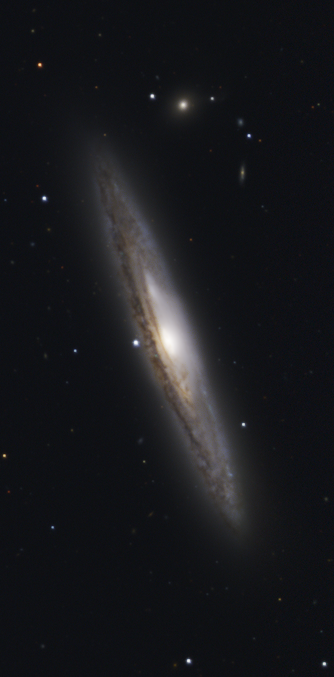
\includegraphics[width=0.49\textwidth]{../Images/chapter_1/SN2024gy_pre-SN.png}
    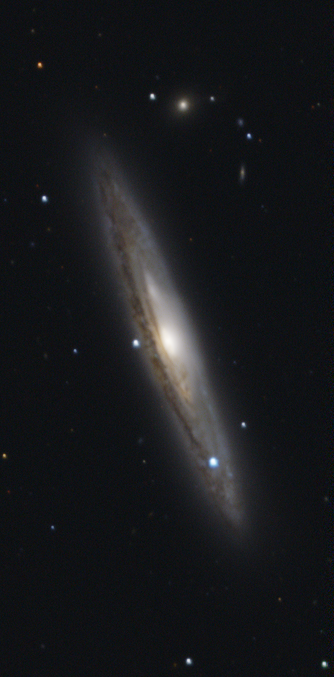
\includegraphics[width=0.49\textwidth]{../Images/chapter_1/SN2024gy_active.png}
    \caption{\ztfg\ztfr\ztfi\ composite image of NGC 4216 using observations taken by ZTF.\\
    \textbf{Left:} composite image of observations taken before 1 January 2024.\\
    \textbf{Right:} composite image of observations taken between 5 and 19 January 2024, the first two weeks after the first detection of the Type Ia SN~2024gy. (Credit: Benjamin Nobre Hauptmann)} %30, 29, 14 (gri SN images) & 35, 31, 30 (gri pre-SN images) given to Benjamin, subset used based on data quality, exact numbers not so relevant
    \label{2024gy_ZTF}
\end{figure}


\subsection{Core-collapse SNe}
\label{CCSN}
As was mentioned at the end of section \ref{ge_8_Msol}, stars above 8 $M_\odot$ end their lives in a CCSN when the core implodes into a compact object due to the effects of gravity. The outer layers fall in as well but bounce back outwards as the enormous amounts of released gravitational energy from the collapsing core is imparted on the outer layers, heating them up and expelling them outwards at high velocities. The light coming from the cooling of this material and the radioactive decay of newly formed unstable nuclei into stable ones cause the SN to rise rapidly in brightness. Within hours after the explosion it is bright enough to be observed in other galaxies, peaking after several days to weeks at an absolute magnitude in the range of -16.5 mag to -18.5 mag depending on the type of CCSN \citep{SN_M_dist}. This is what we observe as the SN event, and by analysing their spectra around peak light they can be classified based on the visible elemental emission and absorption lines.

The composition of the outer layers of the progenitor depends heavily on the life of the star. Most CCSNe have hydrogen in their envelope, which will show up in the SN spectra as strong Balmer P Cygni profiles. These are known as Type II SNe. Photometric features of the light curve (the SN brightness as it changes over time) are also used in SN identification, leading to subtypes such as SN IIL or SN IIP for Type II SNe that show a linear decline or a plateau, respectively. High mass-loss rates, due to a high stellar wind \citep{He-star_pre_SN_evol_mass_loss} or the presence of a binary companion \citep{He-star_pre_SN_evol_binaries}, can however strip the hydrogen layer, leaving the helium shell as the outermost part of the progenitor at the moment of explosion. When there is no hydrogen visible in the spectrum, the SN is of Type I. CCSNe that show no H lines but do have He lines in their spectra are called Type Ib SNe. In some extreme cases even the helium layer has been stripped away, resulting in SNe without H or He lines in their spectra, known as Type Ic SNe. Transitional objects, where a layer is mostly but not completely stripped, are also known \citep{SN_large_pic}.\\

Photometric classification is cheaper as photometry is easier to obtain, but it cannot differentiate between subtypes that are defined on the presence, strength, or absence of specific elemental lines, leading to broader classifications with less certainty. Besides this, many of the differences that make certain SNe interesting are visible at early times, while a SN needs to evolve up to a certain point to have a light curve that can be used for classification. For these reasons, a common strategy is to use dedicated large-scale surveys such as the ZTF to find new SNe within days after explosion using photometry, and using different telescopes to follow these up with spectroscopy for classification.

\subsection{Thermonuclear SNe}
\label{SNIa}
Besides CCSNe are the more commonly observed thermonuclear SNe (Type Ia SNe, SNe Ia), which are exploding WDs after fusion in their core has been ignited through some mechanism (see section \ref{Ia_progenitors}). The more massive the WD, the easier it is to ignite as the nuclei are forced closer together. Since the WD is degenerate, the energy released by a single fusion event can completely be used to heat up the surrounding material and let it fuse as well, leading to a runaway process where the entire WD tries to fuse to iron-peak elements on a timescale of seconds. This process disrupts the entire star, expelling the material outward at relativistic speeds \citep{Ia_thermonuclear}. While not all material in the WD is fused, most of the mass ends up in $\Nififtysix$, with typical SNe Ia producing between 0.3 -- 0.8 $M_\odot$ of $\Nififtysix$ \citep{Ia_Ni56_yield}. This is an unstable nucleus and decays as
\begin{equation}
    \Nififtysix\ \xrightarrow{6.1\text{ d}}\ \Cofiftysix\ \xrightarrow{77.3\text{ d}}\ \Fefiftysix,
\end{equation}
with $\Fefiftysix$ being the stable end product of the decay chain. The key spectral signatures of a SN Ia are the absence of hydrogen lines and broad \SiII\ absorption features in their spectra around peak brightness. At first, the ejecta are dense and opaque, and only photons from the outer layers can escape. As the ejecta expand, they become more transparent, and the slower moving inner layers become visible as the photosphere recedes inwards through the layers. Therefore, by taking spectra at different phases, a map of the elemental abundances in velocity space can be built. As different models of the progenitor system and explosion mechanisms predict different compositions, this is a popular way to compare models to observations \citep[e.g.][]{ptf11kx,de_2019_18byg,2020sck_Iax,2021rhu}.

The SN reaches peak brightness around three weeks after the explosion and starts to fade again. The main power source that governs the rate at which the SN fades is the decaying $\Nififtysix$, resulting in a linear decline of the light curve in magnitude space. In the near-infrared there is a second peak a few weeks after the first, which is suggested to be the result of a decrease in opacity due to the changing ionization state of iron group elements \citep{2nd_max}. Figure \ref{Ia-norm_example} shows an example of a well-observed normal SN Ia.

\begin{figure}
    \centering
    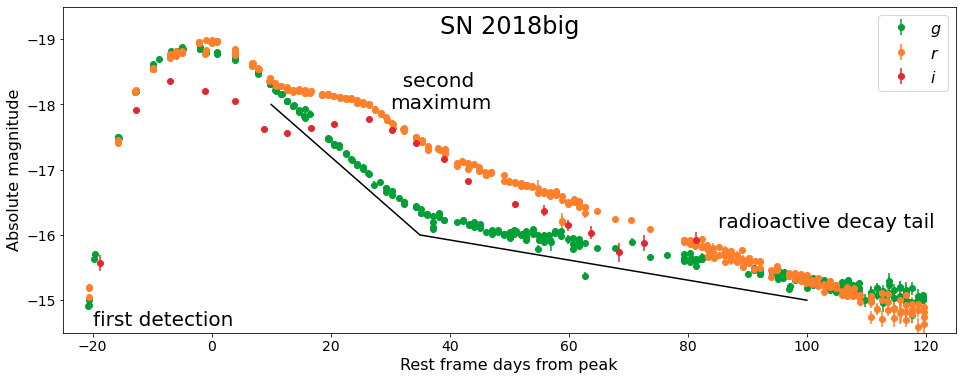
\includegraphics[width=\textwidth]{../Images/chapter_1/Ia-norm_example.png}
    \caption{ZTF \ztfg\ztfr\ztfi\ light curve of a SN Ia in the rest frame and absolute magnitude, corrected for Milky Way extinction but not for host extinction. The \ztfg-band clearly shows a change in the decline rate as $\Cofiftysix$ decay becomes dominant over $\Nififtysix$ decay (as shown by the broken black line). The \ztfr- and \ztfi-band show the second peak.}
    \label{Ia-norm_example}
\end{figure}

\subsubsection{Standardizable candles}
\label{Standard_candle}
Most SNe Ia peak around an absolute magnitude of -19.5 mag, making them brighter than CCSNe. Some SNe Ia become brighter than others, but they also evolve slower. This is called the Phillips relation \citep{phillips_rel}, and it can be used to infer the absolute peak brightness based on how fast it evolves. \citet{Tripp_colour_rel} improved the standardization by adding a second term: the so-called colour luminosity term. This accounts for the intrinsic SNe Ia colour, as bluer SNe Ia are brighter. These days a third term is included, which accounts for environmental dependencies and is implemented as a step function \citep{Kelly_mass_step, Sullivan_mass_step}. The resulting standardization formula is given by
\begin{equation}
    \mu_\text{obs} = m_B - M_0 + \alpha x_1 - \beta c - \gamma p,
\end{equation}
where $\mu_\text{obs}$ is the observed distance modulus. $m_B$ and $M_0$ are the apparent and absolute B-band magnitude, respectively. $x_1$ is the SN stretch, $c$ its colour, and $\alpha$ and $\beta$ are the coefficients used to correct for these effects. $\gamma$ is the size of the step function, and $p$ determines when this step needs to be applied.

Using the standardisable nature of SNe Ia allows their distance to be measured, as well as the distance between Earth and the host galaxies they reside in. At the same time, the redshift of the host galaxy can be measured from the spectra. With these values together, the Hubble constant $H_0$, which measures the expansion rate of the universe, can be measured. The SH0ES team \citep{SH0ES} used the Pantheon+ sample \citep{Pantheon+} to measure the expansion rate of the universe and found it to be $H_0 = 73.30 \pm 1.04$ km s$^{-1}$ Mpc$^{-1}$.


\subsection{Other types of transients}
\label{Other_trans}
There are other types of transients besides the SNe mentioned above. Some SNe become much brighter than normal events and are therefore called superluminous SNe (SLSNe). Supermassive black holes (SMBHs) in the centre of galaxies can cause a variety of transient events such as tidal disruption events (TDEs) or ambiguous nuclear transients (ANTs), or a galaxy could have an active galactic nucleus (AGN). Some types of stars also pulsate, and vary in brightness over time. All of these can show up as transients in surveys looking for changes in the night sky on a day-to-day basis.


\subsubsection{SLSN - Superluminous Supernova}
SLSNe are SNe that have a higher peak luminosity than normal SNe, in some cases reaching over 5 magnitudes brighter than normal events at their peak \citep{SLSN_Gal-Yam}. Like normal SNe, they can be classified into Type I and Type II based on the absence or presence of hydrogen emission lines in their spectra. One of the main puzzles regarding these types of events is the source that powers their superluminous nature. Different types of models have been put forward, using magnetars \citep{Maeda_SLSN_magentar}, black holes \citep{SLSN_BH}, radioactivity \citep{Kasen_SLSN_pair_instab}, or interaction with circumstellar material (CSM) \citep{Late-time_CSM_SLSNE_I} to push the brightness significantly above that of regular SNe. Each of these has different strengths and weaknesses.


\subsubsection{AGN - Active Galactic Nucleus}
An AGN is the central region of a galaxy in which a SMBH accretes matter at a high rate, releasing a part of the potential energy as heat and radiation. As a result of this, the AGN has a very high luminosity compared to the rest of the galaxy, with different orientations of the system resulting in different types of AGN \citep{Antonucci_1993_AGN, Urry_1995_AGN}. As the stream of matter being accreted is inhomogeneous, the accretion rate and luminosity change over time. In some cases AGN variability is so extreme that it changes the entire spectrum of the AGN, with (dis)appearing broad emission lines and continuum flux. These are so-called changing-look AGN (CL-AGN) \citep[see][for a review]{CLAGN}. AGN variability can be used to estimate the SMBH mass through reverberation mapping \citep{Reverberation_mapping, Reverberation_Peterson}. Fast moving clouds close to the AGN change the strength of line emission based on how strongly they are illuminated by the AGN. The delay between a luminosity change in the AGN continuum and the broad emission line features coming from these clouds gives a measure of their distance, while the width of the emission lines gives a measure of their velocity. From these measurements the SMBH mass can be estimated using Kepler's third law.


\subsubsection{TDE - Tidal Disruption Event}
In some cases a star can get too close to the SMBH and get tidally disrupted \citep{Rees_1988_TDE, Strubbe_2009_TDE}. In a TDE the star gets ripped apart due to the strong gravity of the SMBH and forms an accretion disk of hot gas that gets accreted onto the SMBH. The distance at which the TDE occurs depends largely on the SMBH mass, and for SMBHs more massive than $\sim10^8 M_\odot$ the tidal disruption radius lies within the event horizon, meaning that TDEs cannot be observed around the most massive SMBHs \citep{Hills_mass}. The other dependency of the tidal radius is the difficulty to disrupt a star. Compact objects such as WDs are very difficult to disrupt and thus have a smaller tidal radius. A red giant, on the other hand, has outer layers that are very loosely bound to the star, and the star is therefore easier to disrupt at a larger radius, though this might also result in a partial tidal disruption where only the outer layers are stripped while the stellar core survives the encounter. TDEs can become brighter than SNe, with the brightest event ever observed being AT 2021lwx (ZTF20abrbeie, nicknamed "Scary Barbie"), which is thought to be the disruption and accretion of a giant molecular cloud \citep{Scary_Barbie, 2021lwx_Wiseman}.


\subsubsection{ANT - Ambiguous Nuclear Transient}
Some nuclear variability does not quite fit the known classes of AGN or tidal TDEs, showing characteristics of both types of events. These events have been named ambiguous nuclear transients \citep[ANTS;][]{Kankare_ANT, 2020ohl_Hinkle, Hinkle_MIR_ANT_echo, Hinkle_Extreme_nuclear_transients/ANTs, wiseman_ztfants} and rise up quickly, reaching peak brightness within a few weeks before declining very slowly over hundreds of days, although their decline rates are variable.


\subsubsection{Variable stars}
Some stars show variability as well, with the brightness of certain types of stars oscillating by a magnitude or more. The most famous class of variables are Cepheids, whose regular oscillation period of the order of days is related to their absolute magnitude. They are bright enough to be visible in nearby galaxies, which makes them useful to calibrate SN Ia distance measurements when building the distance ladder \citep{Cepheids_Gibson, Cepheids_Saha}. Other types of stars, such as Mira variables, are much more extreme in their change of brightness and have periods $>100$ days \citep{Mira_varibs}.


\section{SN Ia subclasses}
As has been stated in section \ref{Standard_candle}, most SNe Ia explosions evolve in a very similar way with a tight relation between their peak, colour, and rate at which they evolve. These are called normal SNe Ia, or SNe Ia-norm. This name suggests the existence of abnormal SNe Ia besides the normal ones. This is indeed the case, in fact there is an entire zoo of subclasses that have photometric and/or spectroscopic differences from SNe Ia-norm. \citet{Taubenberger_plot} showed the different subclasses of SNe Ia together by plotting their peak absolute B-band brightness as a function of $\Delta m_{15}$(B), which is the difference in brightness in the B-band between the SN at peak brightness and 15 days after the peak in the SN rest frame expressed in magnitudes. This plot is also shown in Fig.~\ref{Taub_plot}.

\begin{figure}
    \centering
    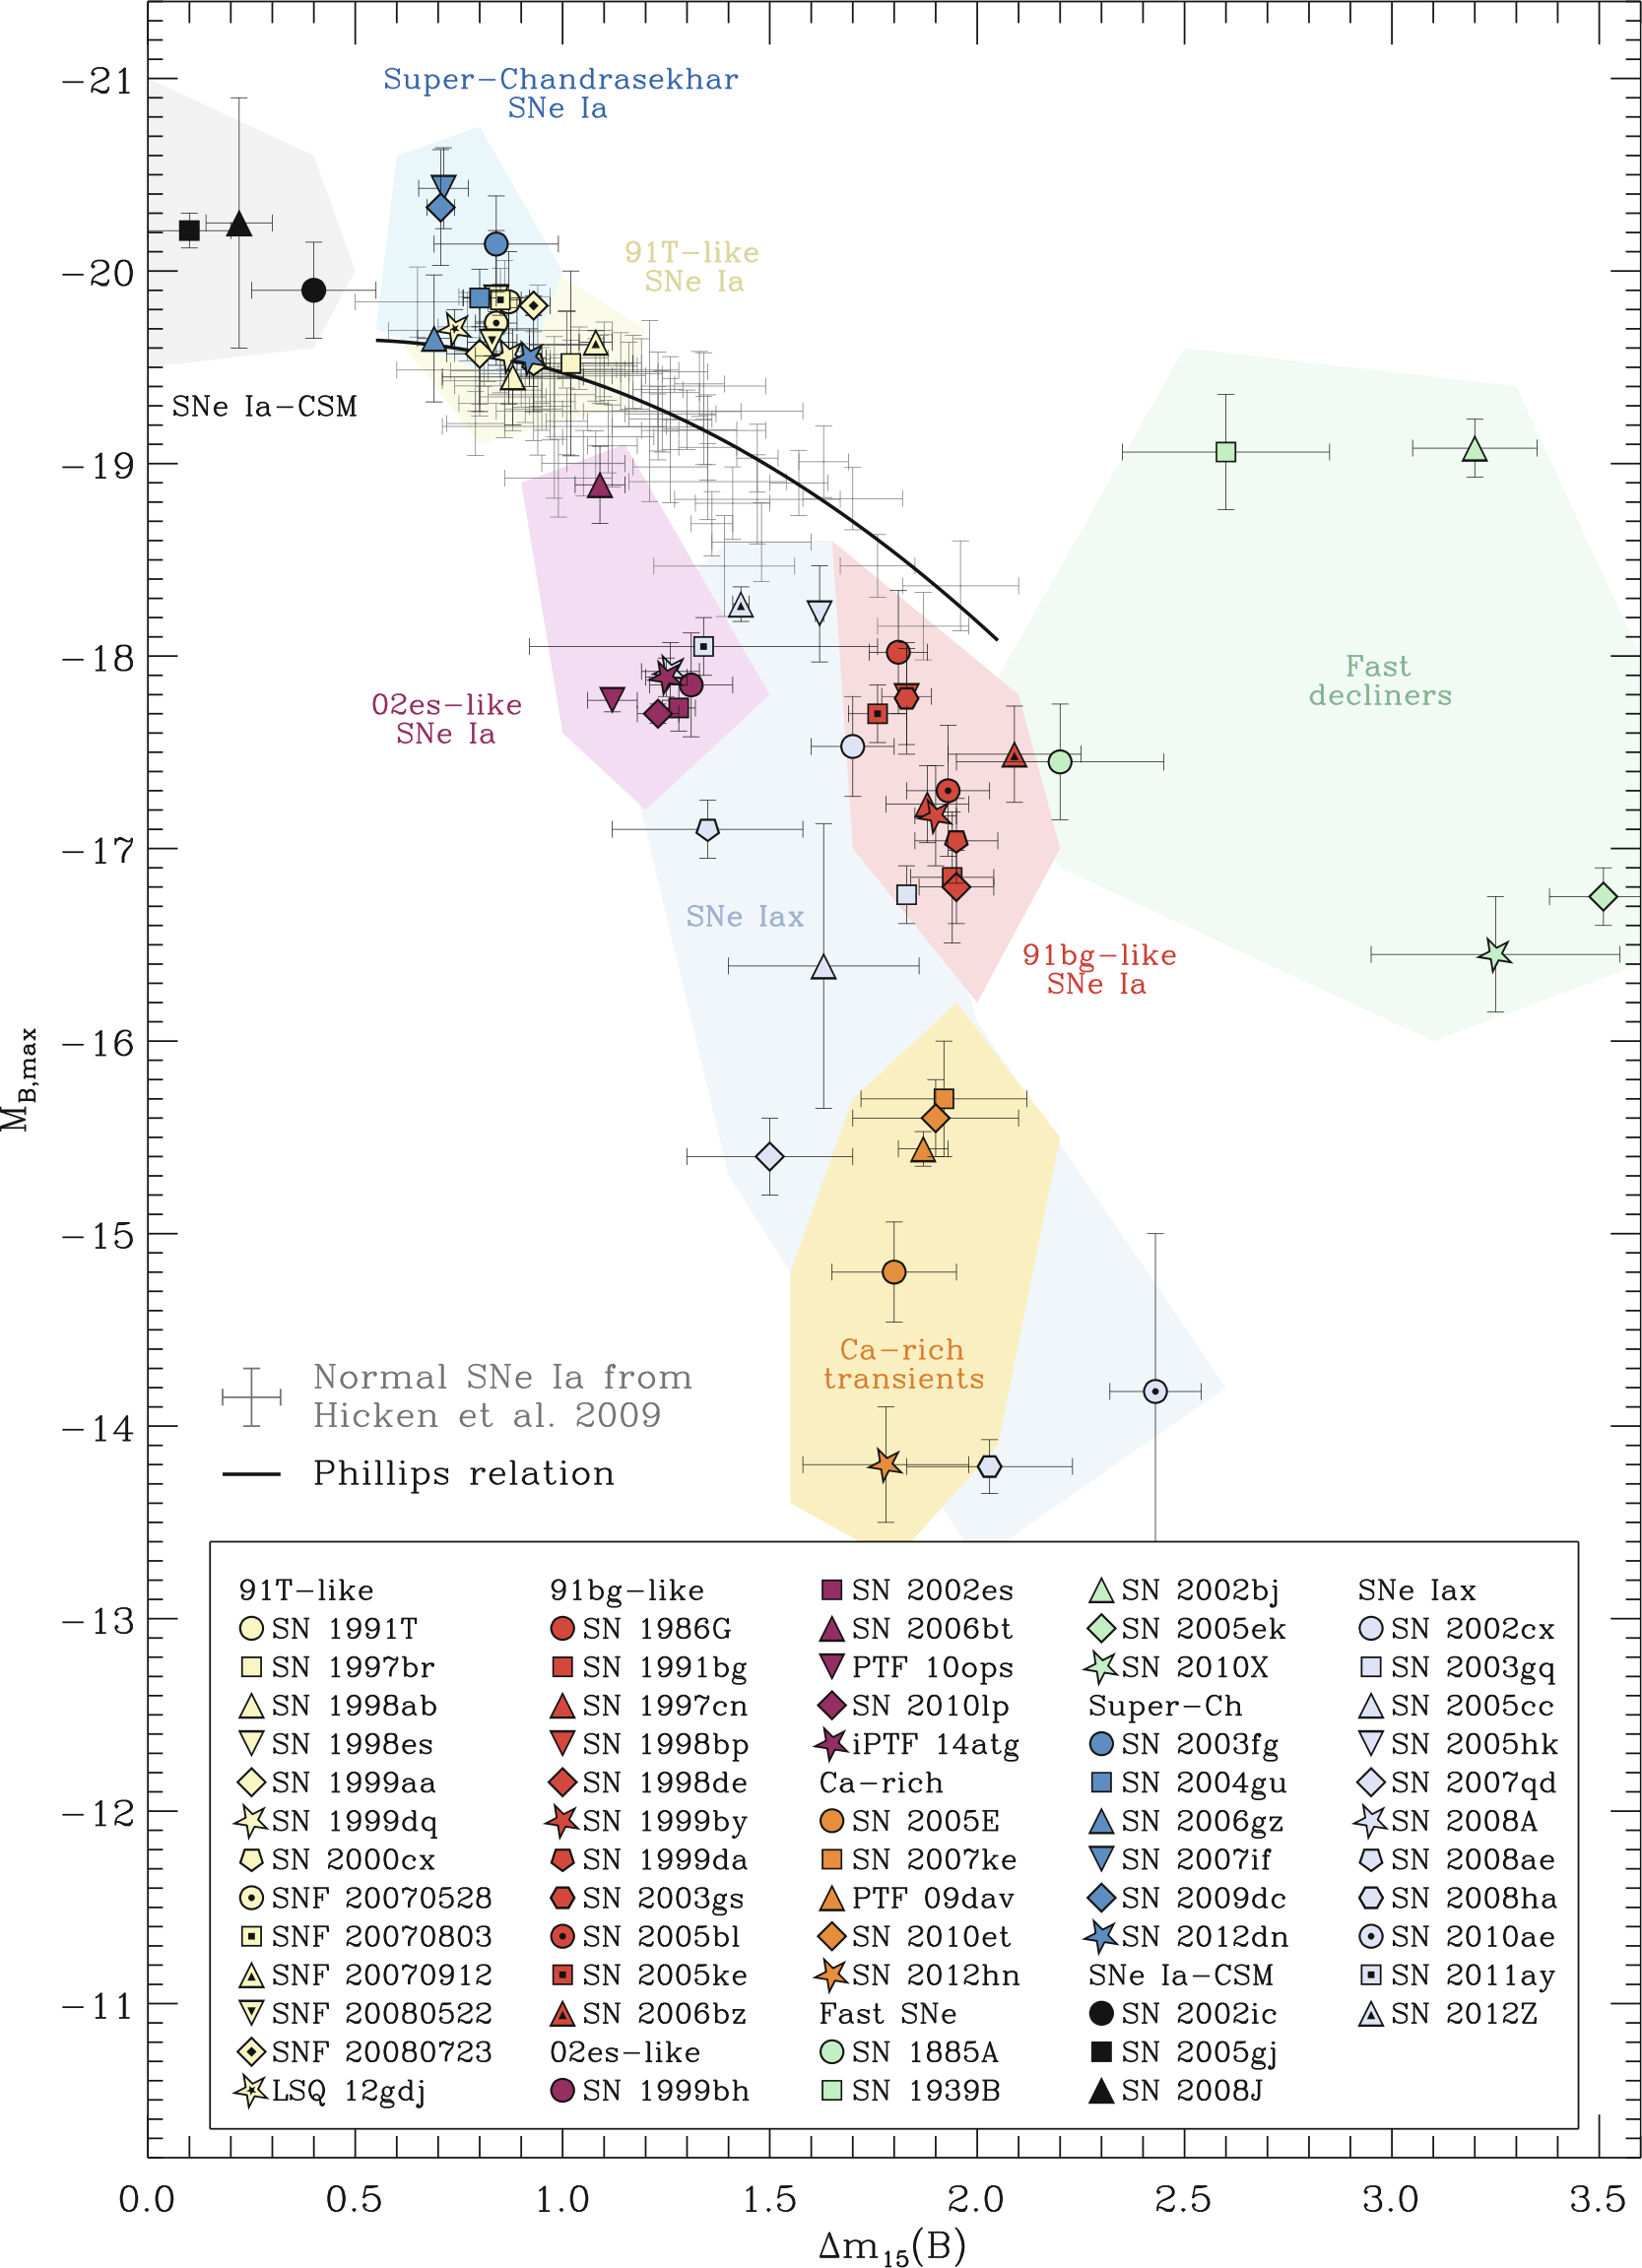
\includegraphics[width=\textwidth]{../Images/chapter_1/Taub_plot.png}
    \caption{Subclasses of SNe Ia. The peak absolute B-band magnitude is plotted as a function of $\Delta m_{15}$ in the same band. Normal SNe Ia lie along the Phillips relation, which is shown with a black line. Most of the non-normal subclasses can be separated from normal SNe Ia based on these two values alone. The main exception are the 91T-like SNe, which form a subclass based on their spectral differences from normal SNe Ia. This figure was taken from \citet{Taubenberger_plot}.}
    \label{Taub_plot}
\end{figure}

Recently, \citet{DR2_diversity} made a similar plot but in the \ztfg-band, using the carefully curated sample of SNe Ia from the Zwicky Transient Facility's second data release \citep[ZTF SN Ia DR2,][Smith et al., in prep.]{DR2_Overview}. They show that $\sim75$\% of all SNe Ia are normal events that can be standardized and used for distance measurements. After that, the two largest subclasses are the SNe Ia-91T ($\sim12$\%) and SNe Ia-91bg ($\sim6$\%), leaving $\sim7$\% as the combined total of various other subclasses.

Different subclasses have a preference for different environments. By studying these, the characteristic properties of their light, and the connection to their environments, we can learn more about the properties of their progenitor systems and the exact mechanisms that are involved in SN Ia explosions.


\subsection{Photometric differences}
The Phillips relation is easily visible in Fig.~\ref{Taub_plot}, and SNe Ia-norm lie in a narrow strip around it. Most subclasses can be distinguished from SNe Ia-norm by photometry alone. The (aptly named) fast decliners fade unusually quickly after reaching peak brightness, while SNe Ia-CSM barely fade at all in the first few weeks after reaching their peak brightness. SNe Iax never reach the peak brightness of a normal SN Ia, which in some models is explained through the explosion failing to fully disrupt the WD \citep{Iax_model_1, Iax_model_2}. Super-Chandrasekhar SNe Ia on the other hand are brighter than what would be expected from a $M_\text{Ch}$ WD explosion. Many subclasses are named after a prototypical SN that defines the subclass.


\subsection{Spectroscopic differences}
Besides photometric differences, most subclasses are also spectroscopically different from SNe Ia-norm. Some have stronger emission lines of particular elements, others have weaker ones. Ca-rich transients \citep[e.g.][]{Ca-rich_2010, Ca_rich_2012, Ca-rich_rate} show \CaII\ emission lines in their nebular spectra that are much stronger than for other SN Ia types. The spectra of super-Chandrasekhar SNe show that their ejecta move considerably slower compared to other subclasses, which, together with their high luminosity, is consistent with a double degenerate merger scenario \citep{2003fg_SuperCh, 06gz_SuperCh, 09dc_SuperCh}.

The SN Ia-91T subclass lies at the bright end of the Phillips relation, and thus cannot be identified photometrically but can therefore be normalized and used for distance measurements. Spectroscopy however reveals that this subclass evolves differently as it rises towards peak brightness, showing a blue pseudo-continuum with two strong \FeIII\ absorption multiplets instead of intermediate-mass element lines. They also have a preference for younger stellar populations \citep{Filippenko_91t, 91T}, although this preference is not seen in \citet{DR2_diversity}.


\section{SN Ia progenitor systems}
\label{Ia_progenitors}
WDs are stable objects on their own, but they can be made to explode under certain circumstances. Not all stars are single, and WDs in a binary system can interact with the other star and start accreting matter coming from the so-called donor star. As the radius of a WD is inversely proportional to its mass (Equation \ref{nonrel_WD_eq}), it will shrink as it becomes more massive until the point is reached where fusion is ignited in the core of the WD, triggering its explosion.

Assuming that the stars have been in the binary system since formation, and since more massive stars have a shorter lifespan, the more massive star has turned into the WD. Therefore, the donor has to be $<8$ $M_\odot$ (though due to stellar and especially binary evolution the mass of the donor has likely changed since formation). The donor could still be burning hydrogen or have evolved to the later stages in its life, up to and including becoming a WD as well. The many possibilities for the donor star is called the progenitor problem, which is currently still being debated. Different progenitor scenarios can broadly be put into one of two categories based on whether the donor star is a compact object (double degenerate) or not (single degenerate). Artistic impressions of these two scenarios are shown in Fig.~\ref{single_double_deg_mods}.

\begin{figure}
    \centering
    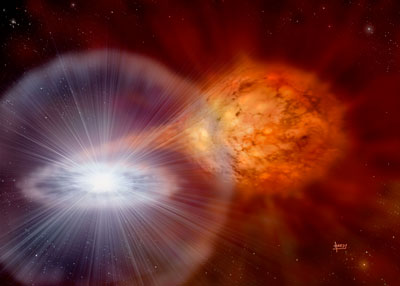
\includegraphics[height=0.229\textheight]{../Images/chapter_1/single_deg.jpeg}
    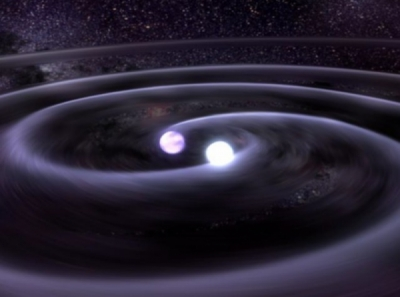
\includegraphics[height=0.229\textheight]{../Images/chapter_1/double_deg.jpeg}
    \caption{\textbf{Left:} Artistic impression of a single degenerate system, where the white dwarf accretes material coming from the surface of the donor star. Image credit: STFC / David Hardy. \textbf{Right:} Artistic impression of a double degenerate system where two white dwarfs spiral in to each other while releasing gravitational waves. Image credit: NASA / Tod Strohmayer (GSFC) / Dana Berry (Chandra X-Ray Observatory).}
    \label{single_double_deg_mods}
\end{figure}


\subsection{Single degenerate}
The most straightforward and classical way to explode a WD is by adding mass to a near-$M_\text{Ch}$ WD until carbon is ignited in the core due to compressional heating. The companion star fills its Roche lobe, and material from the outer layers is syphoned onto the WD. The donor can fill its Roche lobe while it is still a main sequence star, when it has evolved into a red giant, or it may even be a helium star whose hydrogen layer has been stripped due to binary interactions \citep{Whelan_classical_Ia_mod, Nomoto_single_degenerate}. In delayed-detonation models the WD first expands during a deflagration phase, which then transitions into a detonation after the WD becomes unbound \citep{Kholov_Del_det, Mazzali_common_mechanism}.

It is also possible that the WD and red giant companion enter a common envelope phase. The WD merges with the hot core of the red giant, forming a rapidly rotating, WD-like degenerate core with $M_\text{core}>M_\text{Ch}$ inside the red giant. The angular momentum prevents the core from collapsing in on itself but it is gradually lost until it can no longer support itself, triggering the SN Ia explosion in the so-called core degenerate scenario \citep{Kashi_core_deg}.


\subsection{Double degenerate}
If both objects are WDs, the primary (more massive) WD can still accrete material from the secondary WD in a stable Roche lobe overflow scenario \citep{CO_accretion_II, CO_accretion_I}. In non-classical models, a sub-$M_\text{Ch}$ WD can explode by first slowly accreting and building up a layer of helium on its surface, which explodes after a sufficient amount of material is gathered. As this explosion wraps around the outside of the WD, it sends a shockwave into the interior of the star, which culminates near the centre and temporarily increases the local pressure. If this is enough to ignite carbon fusion, the second detonation is triggered, which disrupts the star and results in the main SN \citep{Taam_ddet, Livne_ddet, Shen_ddet, Fink_ddet}.\\

In other scenarios the WDs fully merge, either dynamically or violently. In the dynamical scenario the WDs lose angular momentum as it is radiated away through gravitational waves \citep{Iben_Double_degenerate, Webbink_Double_degenerate}. An artist's impression of this scenario is given on the right side of Fig.~\ref{single_double_deg_mods}. As the WDs come closer, the less massive companion fills its Roche lobe, and material starts flowing onto the primary. As the companion loses mass, its radius increases, leading to more mass loss until the entire star is disrupted. Around half of the material forms a disk around the surviving WD while the rest falls directly onto its surface. Very little material is expected to be flung out of the system. As the system evolves, it eventually explodes in a SN Ia.

In collisions or violent mergers of two WDs a detonation can occur during the merger at the location of the accretion stream due to its high density and temperature \citep{Rosswog_merger, Pakmor_merger, Pakmor_merger2}. This might either directly start carbon fusion at the ignition site or cause a surface explosion that again wraps around the WD and compresses its interior causing a second ignition, depending on the system and WD masses. The asymmetry of this system when it explodes is expected to cause significant asymmetry in the ejecta and its composition in different directions. This is expected to lead to different amounts of polarization of the SN light, depending on the angle between the plane of rotation and the line of sight \citep{Wang_merger_pol, Bulla_merger_pol}.


\section{SNe with circumstellar material}
The progenitor system of a SN is not completely isolated. Through mechanisms such as high stellar winds or binary interaction, a significant amount of material can end up close to the explosion site before the explosion occurs. This is called circumstellar material (CSM), and since it usually originated from the progenitor system, CSM can give new insights into the history of the progenitor system and the sequence of events that led it to explode.\\

Ejecta from the SN explosion are expelled at high velocities and quickly catch up with the much slower moving CSM. As the ejecta slam into the CSM, shockwaves are produced and energy is deposited into the CSM, which starts to emit light of its own. This new light source alters the light curve, making it brighter and slowing or even stalling its decline. CSM interaction also shows up in the spectra as emerging narrow emission lines that give clues about the composition of the slower moving material. Eventually the ejecta overtake the CSM and its signal fades as the CSM is swept up.

Another way in which the presence of CSM has been inferred is through the presence of narrow, time-varying absorption lines, indicating that they evolve alongside the SN \citep[e.g.,][]{2006X, Sternberg_NaID}. However, these absorption lines are not always seen, and their behaviour varies from object to object, making it difficult to interpret them consistently. Light echoes can also provide an opportunity to study circumstellar and interstellar material, though the difficulty to geometrically separate them from the SN location and their weak nature makes this only possible for SNe in the Milky Way or nearby galaxies \citep{Patat_light_echoes, Tycho_Brahe_classif, 2012cg}.

\begin{figure}
    \centering
    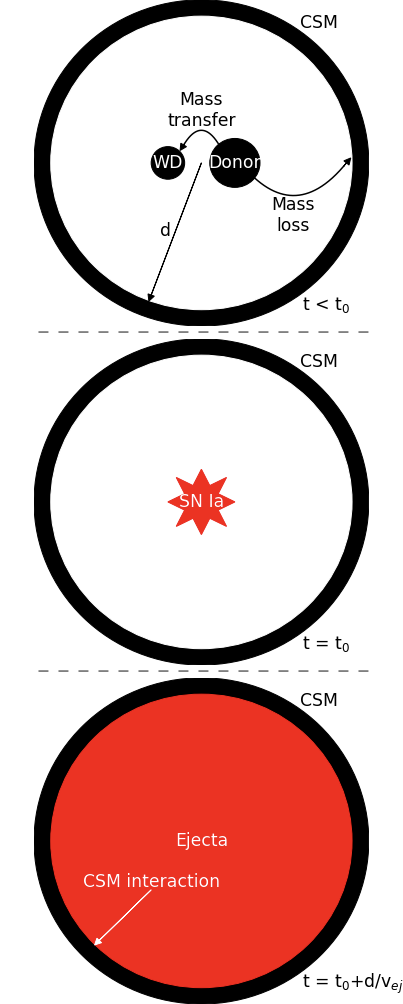
\includegraphics[height=0.847\textheight]{../Images/chapter_1/CSM_sketch_vert.png}
    \caption{Schematic view of a SN Ia-CSM event. \textbf{Top:} The progenitor system containing a WD feeding on material from the donor star. Through various mechanisms a fraction of this material can be lost from the system and end up as CSM in a disk or shell at a distance $d$ around the progenitor system. \textbf{Middle:} The WD explodes as a SN Ia. This can be a SN Ia-norm or a peculiar object, depending on the progenitor system. The ejecta start travelling outwards from the explosion site. \textbf{Bottom:} The ejecta catch up to the CSM and start interacting with it, causing the CSM to start emitting light as well as it is swept up. This results in a slowing down of the photometric light curve decline and the emergence of narrow emission lines in the spectra.}
    \label{Ia-CSM_mod}
\end{figure}

CSM can be created by different mechanisms depending on the progenitor system, and its composition depends on the type of donor star present. In the single degenerate scenario, CSM rich in hydrogen can be created by a WD generating a fast wind, blowing away a part of the material it received from the mass transfer \citep{single_degen_CSM_gen}. In the double-degenerate scenario, part of the tidally disrupted secondary WD becomes unbound from the system, creating (H-poor) CSM and may be able to produce detectable signatures depending on the time between the tidal disruption and the SN Ia explosion \citep{Double_degen_CSM_gen}. The core degenerate scenario could provide a massive amount of hydrogen-rich material near the explosion site \citep[e.g. for SN 2014J,][]{2014J_core_deg}, though the signatures of this scenario could be ambiguous with interacting SNe IIn, leading to confusion \citep{Inserra_2016}. \citet{snips} proposed that the core degenerate and double degenerate scenarios could lead to SNe Ia exploding inside planetary nebulae, possibly resulting in observable time-varying \NaID\ absorption lines or CSM interaction.

Figure \ref{Ia-CSM_mod} shows a schematic view of the creation of a CSM shell (or ring depending on how mass is lost from the SN Ia progenitor system) and the subsequent interaction between the CSM and SN ejecta. When the SN explodes the ejecta will initially expand within the gap between the progenitor system and the CSM, and its spectrum will look like that of a non-interacting class of SN Ia that may or may not display absorption features caused by the CSM if it is in the line of sight. Compared to the ejecta, which are travelling at $v_\text{ej}$, the CSM is practically stationary but at a distance $d$ from the explosion site. This means that the ejecta need a time $t=d/v_{ej}$ to reach the CSM and start to interact with it. Only then does the event transform into a SN Ia-CSM with new narrow emission lines. This later transformation explains why in some cases objects are reclassified as Ia-CSM after first being classified as something else (e.g. SN 2020aekp, which was first classified as a SN Ia by \citealt{2020aekp_1st_classif} but reclassified as a SN Ia-CSM by \citealt{2020aekp_reclassif}).


\subsection{The SN Ia-CSM subclass}
\label{Ia_CSM}
SNe Ia-02ic, also known as SNe Ia-CSM, are the subclass of thermonuclear explosions that show signs of CSM interaction. This often shows up as a peculiar long-lived light curve along with narrow Balmer emission lines, which is a clear indicator of this signal coming from CSM as SNe Ia are expected to be hydrogen-poor. The prototypical event, SN 2002ic, showed narrow \Halpha\ and \Hbeta\ lines, and the slowly declining light curve was found to be consistent with $\sim1.3$ $M_\odot$ of CSM \citep{02ic_H_det, Hamuy_02ic, 02ic_slow_decay, single_degen_CSM_gen}.

Currently, there are several dozen known SNe Ia-CSM \citep{2005gj, Ia-CSM_Silverman, Ia-CSM_BTS}. In all cases the interaction started within two months after the explosion, leading to their (re-)classification after spectroscopic confirmation. The amount and duration of interaction varies quite significantly from one object to another. While some members such as SN 2018gkx and SN 2020xtq mainly feature an unusually slow decline rate, other objects such as SN 2020aekp have a plateau for several 100 days before starting to fade away slowly \citep{Ia-CSM_BTS}.

SN 2011km (PTF11kx) is a well-observed SN Ia-CSM event that shows signs of a complex CSM consisting of multiple shells with which the SN ejecta interact. \citet{ptf11kx} show that its photometry is similar to 91T-like objects before the CSM interaction begins, and explain SN 2011km using a symbiotic nova progenitor system. \citet{Ia-CSM_and_91T_connection} also suggested a link between SNe Ia-91T and SNe Ia-CSM as they show similarities in their peak brightness and spectroscopy before the start of the interaction. In some cases, a 91T-like SN could start interacting with CSM hundreds of years after the explosion, as has been suggested for Kepler’s SN \citet{Kepler_91T, Kepler_CSM}.

Another interesting SN Ia-CSM is SN 2020eyj, which \citet{Kool_He_CSM} present as the first detection of a SN Ia-CSM interacting with He-rich material. Up until then all members of the subclass had shown strong \Halpha\ emission and weak He signatures. SN 2020eyj, however, showed little to no H present in the CSM. This suggests that the progenitor system contained a He star. This was also the first time a SN Ia was detected in the radio. Non-detections in normal SNe Ia suggest a clean environment for the ejecta to expand in, while in this case there is a lot of material present.


\subsection{CSM in CCSNe}
Some CCSNe show interaction with CSM as well. The events are subclassified as SNe~IIn, SNe Ibn, or SNe Icn, with the `n' for narrow emission lines. As stated in section \ref{CCSN}, the difference between these three main types of SNe is the amount of material that has been stripped prior to explosion. Mass can be lost through binary interaction stripping away the outer layers of the star prior to explosion \citep{Ic_binary_progenitors}. Massive stars have also been known to have strong stellar outflows and winds. The existence of Wolf-Rayet stars shows that very massive stars can lose their entire hydrogen envelope, and they are thought to be one of the very last stages in the life of the star before it explodes in a SN Ib or SN Ic \citep{WR_as_progenitors, 2019hgp}. Current models prefer the binary scenario due to the low amount of confirmed disappearances of progenitor stars \citep{CCSN_disappeared_progenitor}.

The CSM often resides close to the progenitor and can be thick enough to obscure features of the underlying SN, depending on the geometry and orientation of the system \citep{1994W, PTF11iqb}. The short distance between the SN and CSM suggests that the material was ejected recently, and in some cases precursor events have been observed prior to the final SN explosion (e.g. SN 2011ht, \citealt{2011ht} and SN 2020pvb, \citealt{2020pvb}). CSM residing close to the progenitor causes most interacting CCSNe to show signs of CSM interaction almost immediately after the explosion. However, examples of the interaction starting much later have been found as well, suggesting that their CSM has been ejected a long time ago \citep{2008iy, late-CSM_IIn_Spitzer}.

Recently, SN 2021yfj was discovered to be a new type of SN and given the classification of SN Ien \citep{Ien_class}. This object showed highly ionized silicon, sulphur, and argon lines but barely any carbon, oxygen, helium, or hydrogen. This suggests the progenitor was a massive star stripped all the way down to its final layer before the iron core. The classification leaves space for the yet-to-be-discovered explosion of a slightly less stripped star in a SN Type Idn, which would have no carbon but strong oxygen, neon, and magnesium emission lines, as well as their non-interacting counterparts and transitional objects. \citep{Ien_disc}.\\


\subsection{Distant CSM}
As stated in section \ref{Ia_CSM} and shown in Fig.~\ref{Ia-CSM_mod}, there is a delay between the SN explosion and the start of CSM interaction due to the distance between the progenitor system and CSM. All objects that are currently classified as SNe Ia-CSM on the Transient Name Server (TNS)\,\footnote{\url{https://www.wis-tns.org/}} have shown signs of interaction at or around peak brightness. Assuming an ejecta velocity of $v_\text{ej} \sim 20\,000$ km s$^{-1}$ and that the interaction starts on average around the SN peak $\sim3$ weeks after the explosion, the CSM is located at a distance $d\sim3.5\times10^{15}$ cm of the progenitor system \citep{Ia-CSM_BTS}. If however the CSM is at a distance of $d\sim10^{17}$ cm, ejecta with the same $v_\text{ej}$ would need $\sim1.5$ years to catch up and start interacting.

In the effort to systematically search for such late-time CSM interaction, \citet{2015cp} looked at old ($\geq1$ year) SNe using the \textit{Hubble Space Telescope} (HST). They focused their search on subclasses that are associated with CSM interaction, such as SNe Ia-91T \citep{Ia-CSM_and_91T_connection}. Out of 72 targets, only ASASSN-15og and SN 2015cp were found to show late-time CSM interaction. ASASSN-15og is a SN IIn with detected CSM interaction around its peak, and was used as a control object. SN 2015cp has been classified as a SN Ia-91T without signs of CSM interaction around its peak. This showed that late-time CSM interaction may be systematically missed due to SNe~Ia not being actively followed at these phases. From a progenitor point of view, this means that material can be ejected from the system prior to the explosion, giving it time to travel further before being caught up by the SN ejecta.

\citet{GALEX_Late_CSM} used archival UV-band data from the \textit{Galactic Evolution Explorer} (GALEX) to look for late-time CSM interaction in SNe Ia. Out of a sample of 1080 SNe Ia, 4 were detected in the UV near peak, but none showed signs of late-time CSM interaction. They show that this type of CSM interaction is rare, occurring between 500 to $1\,000$ d after the initial discovery of the SN in $<5$\% of the SNe Ia at a strength similar to SN 2015cp, and a decreasing percentage as the interaction gets stronger.


\section{In this thesis:...}
In this thesis I will present my work on the search for signs of late-time interaction in SNe Ia using observations taken by ZTF. CSM is connected to the mass loss history of the progenitor system, and more distant CSM has been ejected a longer time ago. By studying late-time CSM it is possible to learn more about the mass loss history of the progenitor system, and it can hold clues to the type of progenitor scenario that the system belonged to.\\

In chapter \ref{chap:obs} I will introduce ZTF as well as the other facilities that have been used to gather data that is presented in this thesis. I will also give an overview of the basics of observing, some of the types of data that can be obtained, and the basic steps that are required to reduce them to something that can be used in further analysis.

Chapter \ref{chap:DR2_search} is an adaptation of \cite{Terwel_2024_paper1}, and presents my search for late-time signals in the ZTF SN Ia DR2, which consists of $3\,628$ spectroscopically classified SN Ia that were first discovered between March 2018 and October 2020. It also details the pipeline and analysis tools I developed to search in a consistent manner (Section \ref{DR2_analysis}).

It might be possible that a late-time signal is observed by ZTF while the main transient occurred before the survey started. In chapter \ref{chap:pre-ZTF_search} I search for this type of event using a slightly modified version of the pipeline used for the DR2 search. As the analysis is exactly the same whether the original transient was a SN Ia, SN II, or any other type of transient, I search through a sample of 8707 transients that were first discovered between 1 January 2008 and 1 January 2018.

Up to this point my search has been through archival data only, with the obvious drawback that it is very likely that any recovered late-time signal cannot be followed up on. By further modifying the pipeline, I search in chapter \ref{chap:Real-time} for late-time signals in SNe Ia in real-time using the latest ZTF observations with the goal to follow up photometrically and/or spectroscopically using other telescopes.

Finally, in chapter \ref{chap:Conc_and_fut} I conclude on the results of searching through these three samples and finish with possible continuations of this search, modifications, and possible alternative usages for this or a similar pipeline.

To convert between apparent and absolute magnitude I assume a flat $\Lambda$CDM cosmology with H$_0 = 67.7$ km s$^{-1}$ Mpc$^{-1}$ and $\Omega_\text{m} = 0.310$ \citep{Planck18VI} throughout this thesis.

\end{document}
%!TEX root = ../main.tex
\documentclass[a4paper,oneside,12pt, class=Latex/Classes/PhDthesisPSnPDF, crop=false]{standalone}
\usepackage{setspace}
\begin{document}
\doublespacing
\chapter{Observing in the optical regime}
\label{chap:obs}

\color{red}To do list: Add refs, sometimes slightly confused which tense to use, recheck carefully, opmaak, reference about the LP light pollution restriction laws? mention gain (e$^-$ / ADU conversion) and read noise (mean e$^-$ added per pixel at readout) as well somewhere. \color{black}

Astrophysicists face the challenge of not being able to set up and control their experiments. The universe is our laboratory but all we can do is see or detect the results while often not knowing the exact setup of the experiment. Models are made to explain and predict the behaviour of planets, stars, galaxies, etc. but ultimately observations are needed to compare against and test our models. My work relies heavily on observational data, and in this chapter I will introduce the different types of observations that are used throughout this thesis (section~\ref{observation_types}), telescopes and instruments that are used to obtain these observations (section~\ref{telescopes}), and a quick overview of how to calibrate the raw images and extract useful data (sections~\ref{calibration} and~\ref{reduction}). I will also give a general overview of what to consider when planning observations in section~\ref{considerations}.


\section{Types of obeservations}
\label{observation_types}
All optical observations are, in esssence, images taken by a camera. Light falls onto a pixel on the detector, a charge-coupled-device (CCD), and frees some amount of electrons. The more light that hits the pixel, the more electrons are freed. At readout these electrons are counted per pixel, or group of pixels if binning is applied, and turned into a digital number called a count. During this process there are contributions from different noise sources, but as long as the total count rate is in the linear regime of the CCD there is a linear relation between the received flux and final count. It is then possible to calculate the observed flux from the target by using calibration images. The different types of calibration images are described in section~\ref{calibration} and their usage is explained in section~\ref{reduction} when discussing image reduction.


\subsection{Photometry}
\begin{figure}
    \centering
    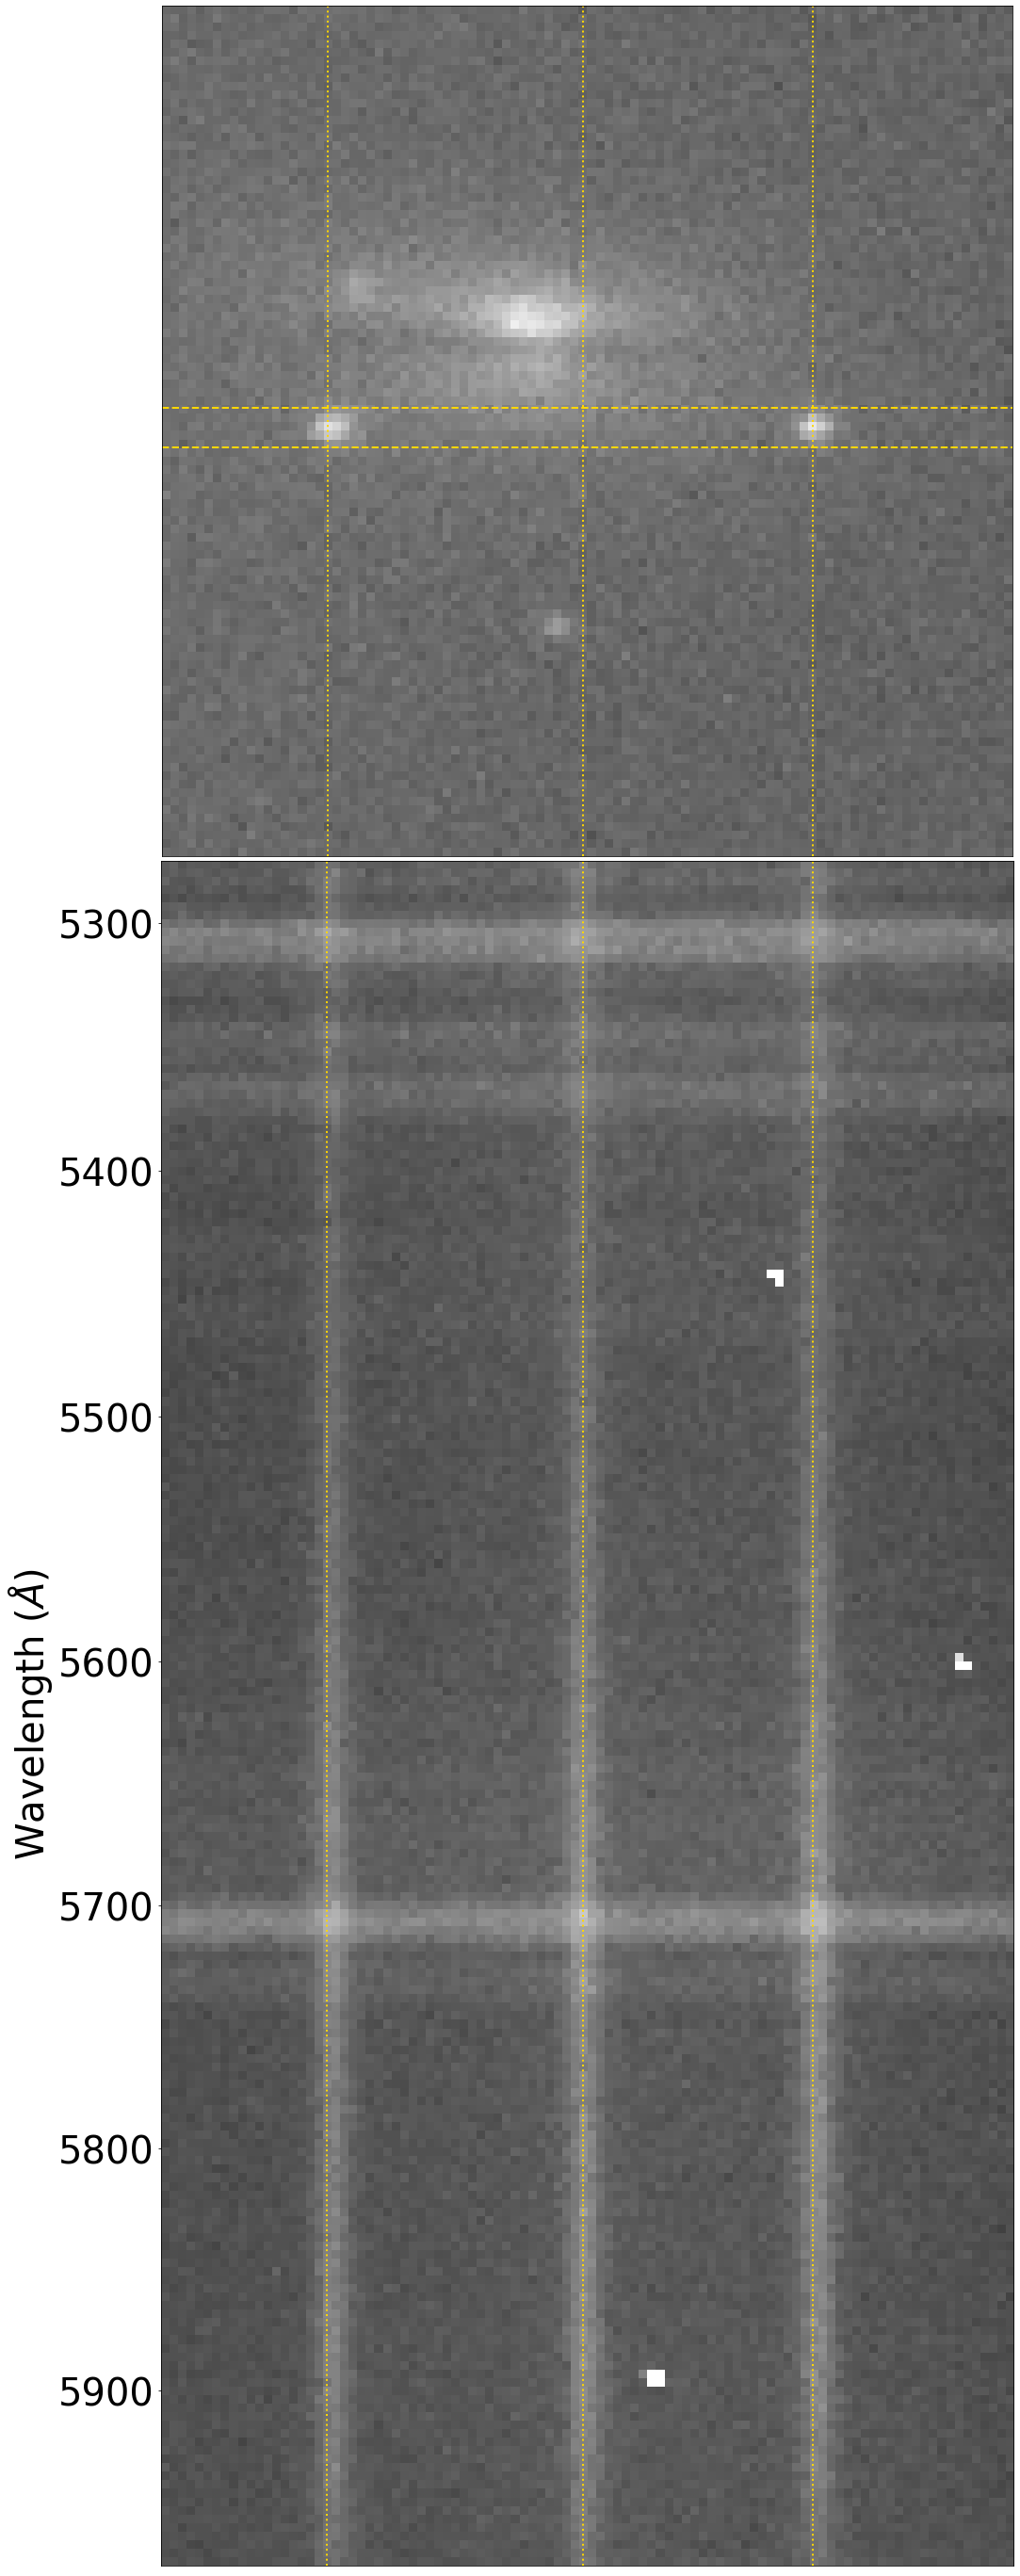
\includegraphics[height=0.8\textheight]{../Images/chapter_2/phot_and_spec_example.png}
    \caption{Image and partial spectrum of SN~2024nqr (left) and SN~2024pgd (right), two SNe Ia active simultaniously in the same galaxy. The image was taken without a filter and used to align the 1.0$\arcsec$ slit (horizontal dashed lines) over both SNe. The resulting spectrum, taken with grism \#4, shows three traces as white vertical stripes. The outer two line up with the two SNe, while the middle trace is from the host galaxy edge in the slit (vertical dotted lines for guidance). The horizontal lines in the spectrum are sky lines coming from atmospheric emission, and the white spots in the spectrum are due to cosmic rays. This data was taken with NOT+ALFOSC on the night of 28 July 2024 while testing an experimental rapid response mode (RRM, credit: Samuel Grund S\o rensen). \color{red}check AT/SN status weirdness \color{black}}
    \label{phot_spec_example}
\end{figure}


Photometry is one of the simplest observing modes as it is just taking a photo of a part of the sky. The top of Fig.~\ref{phot_spec_example} shows a raw photometric image, taken with ALFOSC on the Nordic Optical Telescope (NOT) without the use of a filter. The images are monochromatic, i.e. they only have a value for the intensity. For colourful images multiple observations have to be made using different filters and combined to represent different colours. Faint objects can be observed by increasing the exposure time in a single image, or by stacking multiple images together to increase the effective exposure time. Stacking images can be useful for e.g. reducing cosmic ray interference, avoiding overexposure of a bright source close to a fainter target, or for constructing time series. When stacking images it is common practice to dither the telescope: applying a small offset between exposures to ensure that the target hits a different part of the CCD to avoid issues with bad pixels ruining otherwise good observations. While this decreases the effective size of the fully stacked image, as long as the edges are not needed there is no issue.

\subsection{Spectroscopy}
Spectroscopy goes one step beyond just taking a photo. Assuming that this is slit spectroscopy, instead of a filter to select a wavelength range to observe now a slit restricts the observable region of the sky to a narrow band along one axis of the detector (e.g. horizontal). After the slit the light hits a grating or grism (a grating and prism combined) which diffracts the light based on wavelength across the second axis of the detector (vertical). The rule density on the grating / grism dictates the wavelength spread of the light: the more rules per unit distance, the bigger the diffraction, and the higher the spectral resolution of the resulting image. The tradeoff is that a smaller part of the spectrum can be observed at a time, and there is less light being received per pixel which reduces the SNR unless the exposure time is increased to account for this. Any point-like source that is observed becomes a line in the spectral direction, called a trace. Extended sources create extended traces.

There is some freedom in the orientation of the slit. This is called the position angle of the slit. If there are multiple targets near each other, and they can be in the slit at the same time, the required position angle can be calculated from the two target positions. If there is a single target to be observed the position angle can be anything, but usually the parallactic angle is chosen. In this orientation the slit is perpendicular to the horizon, and prevents losses from differential diffraction (different colours diffracting differently when entering the atmosphere at an angle, \citealt{diff_refrac_atmosphere}). The trace will only be slightly diagonal on the CCD.

The bottom panel of Fig.~\ref{phot_spec_example} shows a section of the spectrum taken of the SNe in the top panel image. The two SNe are drawn out into vertical traces and a third trace belonging to the edge of the host galaxy can be seen in the middle. The horizontal lines are sky emission lines, and while these can technically be used to estimate the conversion from pixel position to wavelength, standardized arc frames will result in a much better wavelength calibration (see section~\ref{reduction}).


\section{Telescopes}
\label{telescopes}
Most of the data used in this thesis comes from the Zwicky Transient Facility (ZTF), and follow-up observations have been made using the Nordic Optical Telescope (NOT), and the Gran Telescopio Canarias (GTC), which will be introduced below. Some additional data comes from other sources, which are listed for completeness. The same filter names (\ztfg\ztfr\ztfi) are used for filters at different telescopes,  which have slight differences. In the rest of this thesis I will use \ztfg\ztfr\ztfi\ to refer to the ZTF filters, unless specified otherwise. \color{red} gotta make sure this is done correctly everywhere \color{black}

\subsection{Zwicky Transient Facility}
\label{ZTF}
The Zwicky Transient Facility (ZTF, \citealt{ZTF_Surveys_Scheduler, ZTF_overview_and_1st_results, ZTF_Science_Objectives, ZTF_Instrumentation, ZTF_Observing_System}) is an optical large-sky survey observing the entire northern night sky above Dec $\approx -30$\degree\ every 2 to 3 nights in three broadband optical filters \ztfg~($\lambda_{eff} = 4746.48$ \AA), \ztfr~($\lambda_{eff} = 6366.38$ \AA), and \ztfi~($\lambda_{eff} = 7829.03$ \AA), which are similar to the well-known SDSS \ztfg\ztfr\ztfi\ filters. The efficiency of these filters is plotted as a function of wavelength in Fig. \ref{Optical_elements_plot}. The survey saw first light in October 2017 and the survey formally began scientific operation in March 2018, and has been running continueously until the time of writing this document.

The observations are made using the $48\arcsec$ aperture Schmidt-type design Samuel Oschin Telescope, which is based at the Palomar Observatory in Southern California. Each exposure is 30 s long, can go a limiting magnitude of $\sim20.5$ mag and covers an area of $\sim47$ deg$^2$ at a resolution of of $1.01\arcsec$ per pixel. The camera is divided in a $4\times4$ grid of CCDs, each of which have 4 readout channels called quadrants. This results in each observation producing 64 separate images, each with their own readout channel identifier (rcid). Similarly, the observed region of the sky is divided into different telescope pointings called fields to ensure that the same region of the sky is observed in the same way each time, aiding with the reduction of the data. This results in each combination of filter, field, and rcid being a set of observations of a particular part of the sky using specific setup.

\begin{figure}
    \centering
    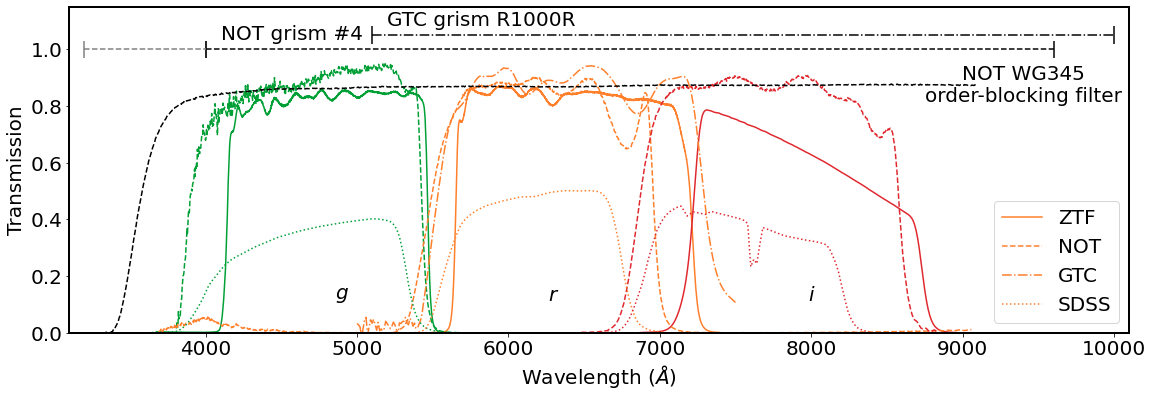
\includegraphics[width=\textwidth]{../Images/chapter_2/transmissions.png}
    \caption{Throughput as a function of wavelength of the different filters used to gather the bulk of the data in this thesis \ztfg\ filters are shown in green, \ztfr\ in orange, \ztfi\ in red, and the different telescopes are shown with different line styles (Continuous for ZTF, dashed for NOT, dot-dashed for GTC). The SDSS filter transmissions (dotted lines) are shown for comparison. For the grisms the wavelength ranges are shown as only, not their efficiency at each wavelength.}
    \label{Optical_elements_plot}
\end{figure}


\subsection{Nordic Optical Telescope}
\label{NOT}
The Nordic Optical Telescope (NOT \footnote{\url{https://not.iac.es}}) is a 2.56 m telescope located at Observatorio Roque de Los Muchacos in La Palma, Spain, at an elevation of 2382 m above sea level. It hosts several instruments for observing in the optical and near infrared, both for imaging and spectroscopy. The \textit{Alhambra Faint Object Spectrograph and Camera} (ALFOSC) was used to obtain the data used in this thesis. I will only discuss the parts relevant to this thesis, further details on this instrument and  details on the other instruments can be found at the NOT website.

ALFOSC is a versatile instrument mounted in cassegrain and can be used for imaging, spectroscopy, and (spectro)polarimtery. As there are several wheels equipped to hold a variety of optical elements, the instrument can switch quickly between different setups between observations. The images can cover up to $6.4\arcmin\times6.4\arcmin$ per exposure at a resolution of $0.2138\arcsec$ per pixel. In this thesis \ztfg~($\lambda_{cen} = 4800$ \AA), \ztfr~($\lambda_{cen} = 6180$ \AA), and \ztfi~($\lambda_{cen} = 7710$ \AA) are used for photometry. For spectroscopy grism \#4 is used to split the light vertically, together with a horizontal $1.0\arcsec$ slit if the seeing was $\leq1.3\arcsec$ or a horizontal $1.3\arcsec$ slit if the seeing was $\geq1.3\arcsec$. Grism \#4 has a resolution of 3.3 \AA\ pixel$^{-1}$ and an wavelength range from 3200 \AA\ to 9600 \AA, but as the response at short wavelengths is poor, the spectra used in this thesis are cut at 4000 \AA. For some spectra an order-blocking filter (WG345) is used as well to avoid second order diffracted blue light to overlap with first order diffracted red light on the detector. The transmission curves of the filters and wavelength range of the grism are shown in Fig.~\ref{Optical_elements_plot}.
%Details on these optical elements are given in Table \ref{NOT_optic_elems}, and they are shown in Fig. \ref{Optical_elements_plot}.

\begin{comment}
\begin{table}
    \centering
    \caption{Optical elements used for observations taken with NOT+ALFOSC and GTC+OSIRIS+. \color{red} Check the $\arcmin$ symbols necessity and make sure to stay consistent \color{black}}
    %\resizebox{\textwidth}{!}{%Scale table to page width
    	\begin{tabular}{ccccc}
    		\hline
    		\hline
    		Filter & $\lambda_\text{center}$ (\AA) & FWHM (\AA) & T$_\text{max}$\\
    		\hline
    		\ztfg$\arcmin$ NOT & 4800 & 1450 & 0.92\\
    		\ztfr$\arcmin$ NOT & 6180 & 1480 & 0.90\\
    		\ztfr$\arcmin$ GTC & 6410 & 1760 & 0.94\\
    		\ztfi$\arcmin$ NOT & 7710 & 1710 & 0.91\\
    		WG345 & 3560 & - & 0.88\\
    		\\
    		\hline
    		\hline
    		Grism & $\lambda$ range (\AA) & resolution (\AA / pixel) & Orientation\\
    		\hline
    		\#4 & 3200$^*$ - 9600 & 3.3 & vertical\\
    		R1000R & 5100 - 10000 & 2.62 & horizontal\\
    		\\
    		\hline
    		\hline
    		slit & Telescope & Orientation\\
    		\hline
    		1.0$\arcsec$ & NOT & horizontal & \\
    		1.0$\arcsec$ & GTC & vertical & \\
    		1.3$\arcsec$ & NOT & horizontal & \\
    		\hline
    	\end{tabular}
    %}
    \begin{flushleft}
    	$^*$ The detector response is limited at low wavelengths, so in practice a lower limit of 4000 \AA\ is used for the spectra in this thesis.
    \end{flushleft}
    \label{NOT_optic_elems}
\end{table}
\end{comment}

\subsection{Gran Telescopio CANARIAS}
\label{GTC}
The Gran Telescopio CANARIAS (GTC \footnote{\url{https://www.gtc.iac.es}}) is a 10.4 m telescope at Observatorio Roque de los Muchachos in La Palma, Spain, and is the largest optical / near infrared telescope on the island. Its primary mirror is made up from 36 hexagonal pieces creating an effective collection area of 73 m$^2$, ideal for observing very faint targets. The GTC can host up to six instruments at a time in various focal positions, allowing for a large variety of observations to be made. One of the most commonly used instruments is OSIRIS+, the upgraded version of OSIRIS: the \textit{Optical System for Imaging and low-Intermediate-Resolution Integrated Spectroscopy}.

OSIRIS+ has an unvignetted field-of-view of $7.8\arcmin\times7.8\arcmin$ at a resolution of $0.254\arcsec$ per pixel. Since the standard readout has $2\times2$ binning, the resolution can be increased to $0.127\arcsec$ per pixel if so desired. Like ALFOSC, this instrument is also built to easily switch between different setups between observations. For photometry the \ztfr~($\lambda_{cen} =6410$ \AA) filter is used in this thesis, and for spectroscopy the R1000R grism with a $1.0\arcsec$ vertical slit is used. R1000R splits the light horizontally over the detector with a range of 5100 \AA\ to 10000 \AA\ with a resolution of 2.62 \AA\ pixel$^{-1}$ These filter transmission curve and grism wavelength range are shown in Fig.~\ref{Optical_elements_plot}.
%Details on the optical elements are given in Table \ref{NOT_optic_elems}, and they are shown in Fig. \ref{Optical_elements_plot}.% ' after the filter?


\subsection{Other observations}
Small amounts of data coming from other telescopes and surveys are presented in this thesis as well. This includes a follow-up observation of SN~2019ldf in Section \ref{sec:late_time_cand} in \ztfg\ and \ztfr\ using the \textit{ESO Faint Object Spectrograph and Camera version 2} (EFOSC2, \citealt{EFOSC2}) imaging spectrograph on the ESO New Technology Telescope (NTT) in La Silla, Chile as part of the extended Public ESO Spectroscopic Survey of Transient Objects+ (EPESSTO+, \citealt{PESSTO}).

To complement ZTF data of several SNe, in chapters \color{red} PUT REFERENCES ONES SECTIONS ARE IN, MIGHT BE DIFFICULT TO DO SECTION SPECIFIC FOR THIS \color{black} optical photometry from the Panoramic Survey Telescope and Rapid Response System (Pan-STARRS, \citealt{Pan-STARRS1}), (intermediate) Palomar Transient Factory (PTF, \citealt{PTF_1, PTF_2}, iPTF, \citealt{iPTF}), All Sky Automated Survey for SuperNovae (ASASSN, \citealt{ASASSN_paper1, ASASSN_catalog}), Asteroid Terrestrial-impact Last Alert System (ATLAS, \citealt{ATLAS}),  and \textit{Global Astrometric Interferometer for Astrophysics} (Gaia, \citealt{Gaia}) are used, as well as near-infrared photometry from the \textit{Wide-Field Infrared Survey Explorer} (WISE, \citealt{WISE}).


\section{Calibration images}
\label{calibration}
Before the observations can be used for science, the images need to be calibrated. This is done using different types of calibration images, each of which measure and correct for different effects of the telescope and detector. Usually these are taken during the day or twilight so no valuable observing time is lost. It is standard practice to take multiple calibration images and use an odd number in the reduction to find median values and remove interference from e.g. cosmic rays, this is called a master image.


\subsection{Bias}
The first type of calibration image is the bias, which is made by reading out the CCD without exposing. The resulting image contains the amount of counts that will be in every exposure regardless of what has been observed or with what exposure time. In other words, measuring the bias can be tought of as measuring the offset to correct for in every other image.

%$B_{ij}$ is the so-called bias, the measured pixel response that is in every observation regardless of the exposure time and amount of light hitting the pixel. The easiest way to measure this value is to take bias frames: observe with an exposure time of 0 with no light hitting the CCD. $F$ and $t$ are 0 which reduces Eq.~\ref{CCD_response} to $R_{ij}(0, 0) = B_{ij}$

\subsection{Dark}
Any detector that is not at a temperature of 0 K will have some amount of noise due to thermal effects. This can free electrons in pixels over time, creating a dark current and increasing the noise over time. The effect can be measured by exposing for the same amount of time as the science images taken, but without letting any light hit the CCD. This is called a dark frame.

As this is a thermal effect, it can be reduced to negligible amounts by cooling the instrument. This saves precious observing time, as otherwise dark frames would ideally have to be taken at the same temperature as the target was observed, which is easiest to do directly after the science exposure. By cooling the detector with e.g. liquid nitrogen this noise source can be avoided instead of having to correct for, saving time and the amount of images that need to be taken in the process.

%Next is $D_{ij}$, the noise that increases with longer exposure times. This is thermal noise, and as its name suggests it is more impactful the higher the temperature $T$ is in the CCD: $D_{ij} = D_{ij}(T)$. Due to this there are actually two ways to remove this source of noise. One can take Dark frames by exposing for some amount of time but making sure no light hits the detector, $R_{ij}(0, t) = B_{ij} + D_{ij} \times t$, and extract $D_{ij}$. This takes however a lot of time, and it is often more efficient to cool the CCD down to very low temperatures (e.g. with liquid nitrogen) to ensure $D_{ij}$ can be neglected.

\subsection{Flatfield}
The amount of light that the telescope receives is converted into a digital number, but there is no guarantee that this conversion rate is the same for each pixel. This can be due to intrinsic differences between the pixels, or outside effects such as dust reducing the amount of light recieved on a part of the detector. To correct for this an evenly illuminated field has to be observed, resulting in an image called a flat or flatfield. By ensuring that each pixel receives the same amount of light, the different counts will reflect the varying responses per pixel.

Any evenly illuminated object can be used for this, such as the the inside of the telescope dome to create dome flats. A more perfect evenly lit source however is the sky, and using this sky flats can be taken. While it is usually too bright during the day and the CCD will saturate even with the narrowest filter and shortest exposure time, there is a window during twilight where the sky is darker but not dark enough to observe stars yet, perfect for taking flats. As a general rule, narrowband filters need a brighter sky and in the evening these need to be done before the broadband filters. After that, assuming similar efficiencies between filters, blue filters need brighter skies than red filters, forcing a specific order in which the sky flats need to be taken during the short window where this is possible. Of course if flats are taken in the morning the order has to be reversed.

%Lastly, to measure $A_{ij}$ flatfield images are needed. During a science exposure the amount of light hitting a pixel is dependent of the brightness of the source at that location, $F = F_{ij}$. But as not every pixel may have the same response the measured values need to be normalized before different pixels can be compared. This is done by observing an evenly lit background where $F_{ij}$ is the same for every pixel. This can be done by observing the inside of the dome (dome flats), although the twilight sky (sky flats) are usually preferred as they are more evenly lit across the CCD.

\subsection{Arc}
In spectroscopy one of the axes has low wavelength at one end and high wavelength at the other end of the image. To know where each wavelength falls on the detector, arc frames are needed. These are taken by observing a lamp filled with a known set of elements (e.g. He, Ne, or TH and Ar). The wavelengths of the emission lines are known very precisely, and by matching these with the observed lines in the arc image a pixel-to-wavelength conversion can be found, called the wavelength solution.

Usually arcs can be taken during the day, when the telescope is idle. However in some cases the mechanical flexure of the telescope, caused by being in a different position during observing, can introduce an uncertainty in the wavelength calibration unless an arc is taken with the telescope in the same position as for the target. In these cases an arc is usually taken directly before or after the target is observed, or between exposures of the target.

%For spectroscopy another type of calibration is needed: Wavelength calibration. This is done with arc frames: observing the known emission lines of several elements using lamps in the instrument (e.g. He, Ne, ThAr lamps) using the same setup as the science observation. The resulting pattern of emission lines is known and can be used to map the pixel position in the spectral direction to a wavelength, called the wavelength solution.

\section{Reduction}
\label{reduction}
After all observations have been taken it is time to analyze them. The first step is to reduce the raw data into the required format to work with. After that, additional analysis technique can manipulate the reduced images directly or the data that has been extracted from them. The response function of a detector can be written as

\begin{equation}
	R_{ij}(f, t, \lambda) = B_{ij} + D_{ij}(t) + F_{ij}(\lambda) \times f \times t,
	\label{CCD_response}
\end{equation}

where $R_{ij}$ is the CCD response of pixel $i,j$ as a function of the integrated flux of the target $f \times t$ during the exposure which lasted a time $t$. The goal is to measure the flux $f$, which requires knowing and correcting for the bias level $B_{ij}$, dark current $D_{ij}$, and pixel response $F_{ij}$. Each type of calibration image is used to measure one of these values. Note that it is assumed that there are no cross or higher order terms in Eq.~\ref{CCD_response}, in other words, the CCD is in its linear regime. When a pixel receives too much light and gets close to saturation it is no longer in its linear regime, and more terms appear in Eq.~\ref{CCD_response} making it much more difficult or even impossible to measure the observed flux.


\subsection{Bias, dark, and flat corrections}
Using the calibration images from section~\ref{calibration}, the raw science images can be reduced to something a flux level can be measured from. 

First the master-bias is created and subtracted from every other image. As both $F$ and $t$ are 0, the bias measures $B_{ij}$ directly and can then immediately be removed.

With the bias gone, the dark frames measure $D_{ij}$ for a specific $t$, but the master-dark can only be used on sciene observations with the same exposure time. Alternatively it is possible to subtract $B_{ij} + D_{ij}(t)$ in a single step by not separating out the bias term using bias images first.

Finally every science image is divided through the normalized master-flat to equalize the pixel responses. There is still a factor $F(\lambda)$ present as the detector efficiency is wavelength dependent, but the value is now indepentent of the pixel position, allowing values from across the CCD to be compared.

\subsection{Cosmic-ray removal and image stacking}
At this point it is often good practice to run a cosmic-ray removal algorith to remove this source of noise as much as possible. This can be done using e.g. L.A.Cosmic \citep{lacosmic}, which I used through Astro-SCRAPPY \citep{astroSCRAPPY} when reducing follow-up photometry of several objects in this thesis.

If multiple images are taken of the same field or object they can be stacked to reduce background noise and increase the SNR of the observed objects. Sometimes the observations have been taken with dithering to avoid the same objects being on the same pixels in every exposure, which has to be taken care of to make sure that the images are stacked correctly.

\subsection{Standard star calibration}
Filters are never 100\% transparent at any wavelength, and the CCD responds differently to different wavelengths as well. To correct for this, one last type of calibration image is used: the standard star. This was not mentioned in section~\ref{observation_types} as observing a standard star is exactly the same as observing the actual science target. The only difference is that the expected result of the observation is known and can be used to correct for the wavelength depent efficiency of the instrument.

With photometry the observed brightness can be measured for each star in the image to get a list of instrument magnitudes. The relative differences between the magnitudes of objects are correct, but there is still an absolute offset across all objects. This is corrected by finding the offset using the standard star. If the filter is commonly used, there is a good chance many stars in the field have known magnitudes in that filter, which can be used for calibration instead of a dedicated standard star.

In spectroscopy the arcs are used to find the wavelength solution for the spectra, after which the trace from the standard star can be extracted and divided by the known spectrum of the star to obtain the sensitivity function of the detector $F(\lambda)$. The trace of the target can be extracted as well to get its spectrum, which can then be flux-calibrated using the sensitivity function. In some cases only a relative sensitivity function is known, resulting in a calibrated spectrum in an unknown flux unit. In these cases proper calibrated photometry of the obect can be used to flux-calibrate the spectrum by integrating the spectrum over the filter transmission curve.


\begin{comment} %USE IMAGE ELSEWHERE?
\subsection{Difference imaging}
Transients are, by definition, objects that appear on the sky for a limited amount of time. A popular and effective way to search for new objects is difference imaging. If there is a map or image of how a part of the sky looked some time ago, it can be used as a reference and subtracted from an image of the current sky. Constant sources such as most stars and galaxies (except variable ones) can be removed. To computers images are nothing more than big matrices. This means that, if properly aligned, subtracting the reference from the science images is an easy operation that leaves only those sources whose brightness has changed between the two observations in the so-called difference image. This also ensures that only the transient light is measured in cases where different sources are superimposed, such as a SN superimposed on top of its host galaxy. Figure~\ref{diff_im_example} shows an example of the resulting difference image after subtracting the reference image from the science image.

\begin{figure}
    \centering
    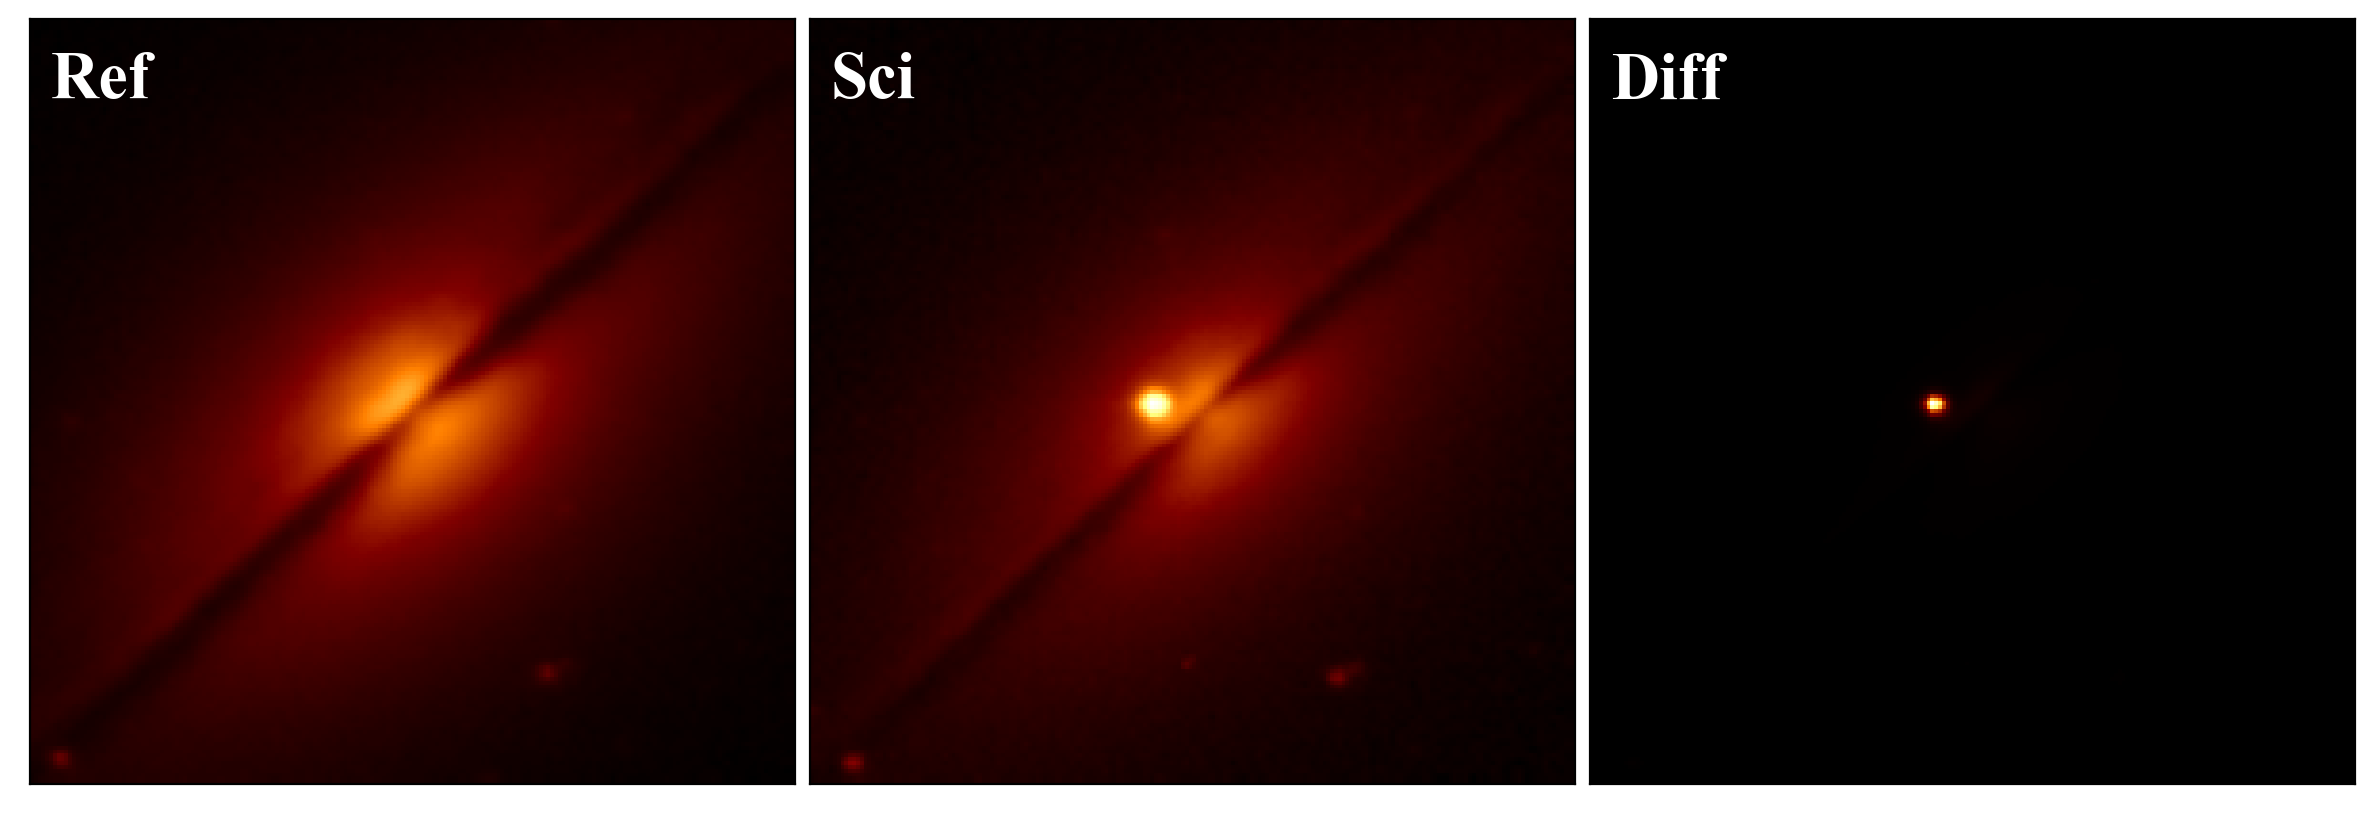
\includegraphics[width=\textwidth]{../Images/chapter_2/diff_im_SN2021rhu.png}
    \caption{Example of a \ztfr-band reference image of NGC 7814, the science image of the same region, and the resulting difference image with the host galaxy removed and only the transient (SN~2021rhu, SN Ia 86G-like) remaining. Credit: Luke Harvey}
    \label{diff_im_example}
\end{figure}
\end{comment}

\subsection{Forced photometry}
The two most common methods to measure flux from as source in an photometric image are PSF photometry and aperture photometry. A good explanation of these can be found in \citet{Photometry_techniques}. PSF stands for point spread function, and with this method a function is fitted to model the source. This function describes how an infinitely small point of light is spread over the detector, and through its spatial size and peak value the flux of the light source can be measured. Aperture photometry sums up the signal in a given radius around the source center and subtracts the contribution from the background in the same region.

%\color{red} See \url{https://coolwiki.ipac.caltech.edu/index.php/Aperture_Photometry_Overview} for references \color{black}

Large surveys such as ZTF observe the night sky to find new transients and monitor known ones. Difference imaging is used to subtract constant sources and reveal active transients, as these are the main sources that should be left in the difference image along with solar system objects that move across the sky. A historically popular algorithm for difference imaging is High Order Transform of PSF ANd Template Subtraction (\textsc{hotpants}, \citealt{HOTPANTS})\footnote{\url{https://github.com/acbecker/hotpants}}, which is used for image subtraction in Sect.~\ref{sec:late_time_cand}. There are other algorithms as well. For instance, ZTF uses \textsc{zogy} \citep{ZOGY}\footnote{\url{https://github.com/cenko/ZOGY}}, and in \color{red}Sect. \color{black} \textsc{autophot} \citep{Autophot}\footnote{\url{https://github.com/Astro-Sean/autophot}} is used to subtract reference images from follow-up observations obtainted with the NOT and GTC.

Through PSF photometry the location and strength of each source in the image is determined, which are then compared to the locations of known sources to separate new from known ones. Each location has however been observed for the entire duration of the survey, which means that it is also possible to measure the flux of a known transient before and after it was visible in the images, creating a light curve for the full duration of the survey.

This is called forced photometry, because the PSF function is forced to center on a specific location instead of finding the best-fitting position for the centroid. All ZTF light curves that are used in this thesis have been obtained through \textsc{fpbot} \citep{fpbot}\footnote{\url{https://github.com/simeonreusch/fpbot}}. When there is nothing but noise at that location the measured flux will be 0 within the error. When there is a source at the target location it will be measured, but if the source is not at the center of the PSF the fit will have trouble converging, resulting in a large uncertainty. Artefacts such as cosmic rays, imperfectly subtracted difference images, or light bleeding effects from saturated bright nearby stars can also affect the accuracy of the photometry measurement.

%\section{The SuperNova Animation Program}
%The light curve that is the result of applying forced photometry at a specific location for the entire run of a survey can contain bad data points. Many of these will be flagged for having a bad PSF fit, bad weather conditions, etc. But even after filtering these out it can be helpful to check the difference images themselves for unexpected behavouir that might be captured in the light curve. For this I created the SuperNova Animation Program (\textsc{snap} \footnote{\url{https://github.com/JTerwel/SuperNova_Animation_Program}})

%\textsc{snap} collects image cutouts of the specified location during the  specified time period(s) and in the specified filter(s). It then matches these with the individual data points in the light curve and puts the images in an animation in chronological order with the reference images at the start. This enables easy identification of bad points due to image defects, off-center sources, residual from imperfectly subtracted sources, cosmic rays etc.

%\section{Simulations}
%Some experiments are difficult or even impossible to do multiple times, one cannot rerun a survey to observe the same transient events. So to understand the biases in the data as well as the effective size of the survey, it needs to be simulated. I used \textsc{simsurvey} \citep{simsurvey,simsurvey_main} \footnote{\url{https://github.com/ZwickyTransientFacility/simsurvey/tree/master}} to simulate an observing campaign like ZTF detecting a specific event under different circumstances. For \textsc{simsurvey} to work both the observer and observed have to be specified, i.e. a model of the telescope, observatory, and survey is required, as well as a model of the transient and where to place it. More details on how the simulation is run are given in section \color{red}ref to paper 1 sim section \color{black}


\section{General considerations for observing}
\label{considerations}
During my PhD I have spent two years doing studentships with the Isaac Newton Group of Telescopes (ING) and Nordic Optical Telescope (NOT) on La Palma, gaining first-hand experience with the specifics of observing in the optical regime and the considerations that come with it. I will briefly go over these in this section. These studentships also gave me the unique opportunity to very quickly follow up on interesting transients, which was very valuable for the objects that will be discussed in \color{red}chapter\color{black}.

%To observe astronomical objects one has to consider several things. Assuming that the location or region on the sky to target is already known, as well as what type of data to collect, an observing plan can be made. A well constructed observing plan should allow to obtain the best quality data possible while making efficient use of the resources available.


\subsection{Location}
Although this is normally already done before constructing a telescope, the first thing to consider is the observing location. When purely aiming for the best observations possible, there are three main things to consider when choosing where to observe from:
\begin{itemize}
    \item {Weather: Clear, stable sky conditions for most nights of the year, and low atmospheric distortion (e.g. seeing) are vital to ensure good quality data on a regular basis. Low hanging clouds can be avoided by being high above sea level, while simultaneously decreasing the amount of air light has to travel through to reach the detector, decreasing atmospheric influence.}
    \item {Light pollution: Darker skies allow observations of fainter objects. Even the the presence of a (partially) illuminated moon significantly changes the depth that can be reached with the same exposure time. Many observatories have (inter)national laws to control the ligth pollution and ensure good quality data can be obtained.}
    \item {Target observability: The target location needs to be reachable by the telescope to be observable. The closer to zenith an observation is made, the less atmosphere between the target and telescope. The atmosphere reduces the data quality through turbulence (seeing), broadband absorbtion (clouds, dust), narrowband interference (tellurics, skylines), and differential diffraction, among others.}
\end{itemize}

Observatories should be located on top of high mountains in areas with stable and clear weather, with as small a nearby population as possible while still being accessible enough for transporting materials and observing staff. One of the best locations in the world that meets these requirements is Roque de los Muchachos on La Palma, a small Spanish island in the Atlantic ocean off the coast of Morocco. At around 2300 m above sea level, the telescopes are built on the highest peak of the mountain far from most communities on the island which are much closer to sea level, and the temperate climate ensures good sky conditions for most nights around the year. Additionally, the government has put laws in place to minimize light pollution, e.g. by limiting the use of street lights and restricting flight paths over the island. \color{red} I remember a plaque at the roque mentioning this, maybe it has a good ref? \color{black}


\subsection{Telescope, instrument, observation type, and setup}
Depending on the type of observations and the brightness of the target there is a choice of hardware to be used. Telescope, intsrument, observation type, and desired setup(s) have to be considered together, as some choices will affect other ones.

Bigger telescopes can observe fainter targets, but it is also more difficult to obtain observing time. On the other hand, smaller telescopes are less oversubscribed (a measure of requested versus available observing time), but are more limited in observation depth even with long exposure times. %Small telescopes are however ideal for bright targets that would instantly saturate the detector of a larger telescope if no filter was used.

Secondly, different instruments, which are often telescope specific, have different observing capabilities. Photometry and spectroscopy are very standard observing modes, and most telescopes have at least one instrument can offer this. Even though ALFOSC and OSIRIS+ can both of these modes, there are still differences in data quality and resolution even if the same object is observed at the same time. However for polarimetric observations for instance, OSIRIS+ cannot be used while ALFOSC can, limiting the options for this observation mode.

Lastly, the specific setup has to be considered as well. For photometry, which filters are desired? If a very specific or rare filter is needed this may limit the options of telescopes and instruments. For spectrocopy there are other choices, such as fiber or slit spectroscopy, different gratings or grisms depending on the desired resolution and wavelength range, neutral density filters to observe targets that are otherwise too bright for the instrument, and order-blocking filters to remove second order blue light from red parts of the spectrum.


\subsection{Night plan}
Lastly, it is good to have a plan of what to observe at each point during the night in order to avoid losing observing time during the night. Most proposals already have a list of targets and standard stars to observe and exposure times when they are submitted to request observation time, but the detailed plan is usually made mere hours before the night starts as it depends on e.g. the current weather, target priority, and specific time constraints (e.g. for transits). Calibration images might need to be taken during the night as well. All of these things need to be concidered when trying to maximize the time used to expose and observe targets, and minimize the overheads from e.g. positioning, target acquisition, and readout.

Time spent repositioning the telescope can be reduced by finding the path between targets that minimizes telescope and dome movement throughout the night. The target acquisition time depends on the type of observation, but also on the experience and tiredness of the observer. With photometry a field is observed, so usually a small offset is not disastrous for the science. With spectroscopy the target needs to be identified and placed in the slit or fiber before the exposure can start, costing extra time. Readout times are detector specific, but can be sped up by windowing and binning if only a part of the CCD is needed, and a worse resolution is acceptable. Considering readout times can be especially important when multiple shorter exposures are taken instead of a single long one.

Nothing is certain during the night. Weather conditions can change suddenly, technical problems can occur, a high priority target can be discovered during the night, or observations might go so smoothly that they are completed faster than expected. A flexible schedule with a priority list and backup targets helps adapting to these situations quickly. After all, an idling telescope in (half-)decent observing conditions is a waste of resources. Fig.~\ref{visplot} shows an example night plan for the NOT with some space for adaptibility built in.

\begin{figure}
    \centering
    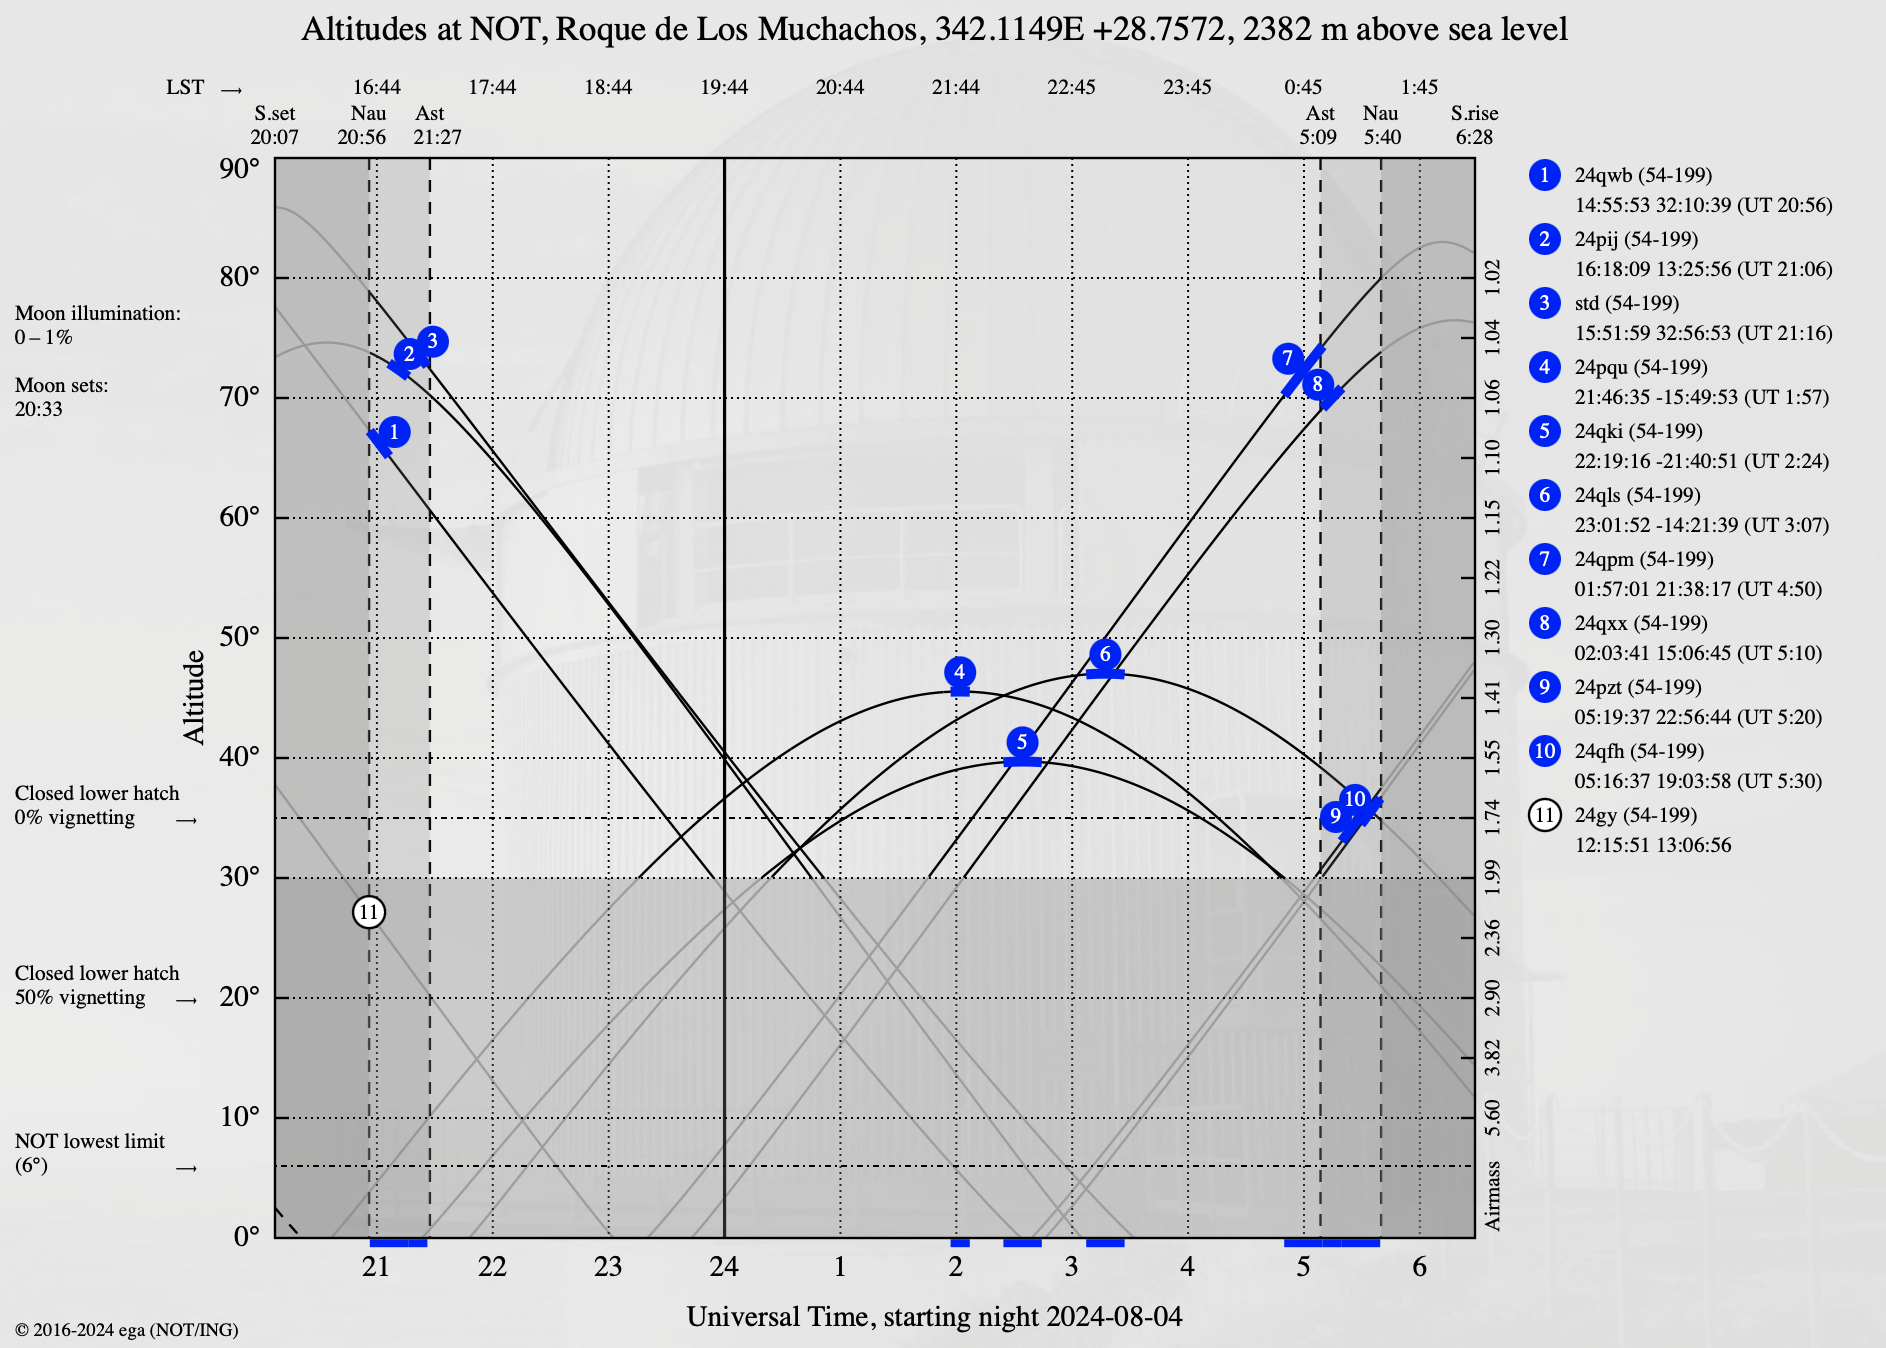
\includegraphics[width=0.95\textwidth]{../Images/chapter_2/visplot.png}
    \caption{Night plan for the NOT on the night of 10 August 2024. Targets are plotted with their altidute as a function of universal standard time. Local stellar time is shown on top. The target priority has been colour coded, with the coloured bars showing the amount of time each observation is expected to take. Green targets have already been completed, and the red vertical line shows the current time. Several unscheduled backup targets are shown in case the plan has to be updated during the night.}
    \label{visplot}
\end{figure}



\end{document}
%!TEX root = ../main.tex
\documentclass[a4paper,oneside,12pt, class=Latex/Classes/PhDthesisPSnPDF, crop=false]{standalone}
\usepackage{setspace}
\begin{document}
\doublespacing
\chapter{ZTF SN Ia DR2: Searching for late-time interaction signatures in Type Ia supernovae from the Zwicky Transient Facility}
\label{chap:DR2_search}


\color{red} This is Paper I, but needs to be properly adapted. Copied starting from Data until the end of conclusions and appended the appendix straight afterwards. To-do list: Check for broken references, check for double refs, reformat pages, add chapter introduction, expand \textsc{snap} section, make sure all the \ztfg\ztfr\ztfi\ things are consistent\color{black}

This chapter details my search for late-time interaction signals in the ZTF second data release (ZTF SN Ia DR2, Rigault et al. in prep.; Smith et al. in prep.) and has been published in \cite{Terwel_2024_paper1}. Chapter~\ref{chap:DR2_search} contains the same details as the paper but expands on Sect.~\ref{snap}. \color{red} Not sure what to put in this introduction, also need to actually expand on the snap section \color{black}


\section{Data}
\label{data}
Our aim is to look for late-time ($>$100\,d after peak brightness) signatures of CSM interaction in the largest sample of SNe Ia to date. This has been obtained by the ZTF. We are particularly interested in events that appear to be normal SNe Ia from their spectra and light curves around the peak but may display signs of late-time interaction, as seen in SN 2015cp \citep{2015cp}. Our starting sample is 3\,628 events that were discovered by ZTF from March 2018 to October 2020 (hereafter the ZTF data release 2, ZTF DR2). Each event is spectroscopically classified as a SN Ia or one of its sub-classes. An overview of the ZTF DR2 will be presented in Rigault et al.~(in prep.), including the sample definition, properties, and use for cosmology. In this study, since we are searching for likely rare signatures of interaction in the ZTF light curves, we are as inclusive as possible in our sample definition and include all SNe Ia in the DR2 covering a redshift out to $z = 0.288$. 

\subsection{ZTF light curve data}
\label{lc_data}
ZTF observes in three optical bands \ztfg\ztfr\ztfi\ on a 2 -- 3 day cadence. Reference images, mainly made using observations at the start of ZTF, are subtracted from the science images using the \textsc{zogy} image subtraction algorithm \citep{ZOGY} to produce difference images. We use forced photometry at the transient location on the difference images using \textsc{ztffps} \citep{ztffps} to get a measure of the observed flux at each epoch. This includes non-detections before each SN was first detected and after each SN has faded below detection limits. 

 Light curve quality cuts on specific light curve points are applied as in Smith et al (in prep.). We do not correct the light curves for Milky Way extinction in our initial analysis but do consider it when focussing on specific objects of interest in Section \ref{results}. 

Another approach for extracting photometry at the transient location is by using Scene Modelling Photometry \citep[SMP;][]{Holtzmann_SMP}. We extract SMP for a few selected objects of interest in Section \ref{results} to test if the identified late-time detections are independent of our approach. When using SMP, one has to define an `off' time and and `on' time. The observations taken during the off time are used to create a model of the region, or scene, where the SN occurs. This is then used as a template during the on time to calculate and remove host contributions to the photometry, leaving just the transient itself (Lacroix et al.~in prep.). The advantage of this method is the significantly lower uncertainty in the model compared to the difference imaging technique, allowing us to find fainter detections. Since we assume that a signal from late-time interaction could occur at any point after the SN, we define the off time as everything up to shortly before the SN explodes, and the on time as everything after this moment.


\subsection{Baseline correction}
 Issues in the construction of the reference images such inaccurate flat-fielding or artefacts in the images that are subsequently co-added can result in a systematic offset in the forced photometry light curve made using different images. The technique of baseline correction is used to correct for this \citep{Yao_baseline_corr,Miller_baseline_corr}. 

To estimate the necessary baseline correction, we calculated the weighted mean of the flux of all data points up to 40 days before the estimated SN peak (which is assumed to be the highest flux detection deemed real), and subtracted it from the light curve. Baseline corrections are done separately for each combination of band (\ztfg\ztfr\ztfi), field (telescope pointing), and rcid (part of the camera, which is arranged in 4$\times$4 charge-coupled devices (CCDs) with four readout channels each, giving a total of 64 readout channels) as each of these combinations uses different, unique reference images. To be able to apply a baseline correction, at least two observations are needed. If this is not possible all observations with that band, field, rcid combination are removed.

Since we are interested in post-SN detections, our baseline correction method using only pre-SN data differs from the one used in Rigault et al.~(in prep.) with both pre- and post-SN data. A comparison between the methods found that for most objects our corrections agree with the ones used in Rigault et al. (in prep.) within the uncertainties. This is as expected as objects with late-time flux excesses are expected to be rare, meaning that the two baseline correction methods should give the same result for most objects. 

If there is insufficient data to perform a baseline correction, the relevant data (based on field, filter and rcid) is removed from the light curve. If this includes data around the peak position, the peak position in the light curve may change and therefore, the position of the peak is recalculated. 


\begin{table}
 \centering
 \caption{Initial sample size and its reduction in each step of the analysis process.}
 \begin{tabular}{lrr}
  \hline
  Criterion & Removed & Objects left\\
  \hline
  Initial DR2 sample & - & 3\,628\\
  No photometry at 100+ days & 109 & 3\,519\\
   No robust late-time detections $^{(a)}$ & 2\,953 & 566\\
  Presence of SN Ia tail $^{(b)}$ & 432 & 134\\
  Removed on visual inspection $^{(c)}$ & 101 & 33\\
  No late-time CSM interaction $^{(d)}$ & 30 & 3\\
  \hline
 \end{tabular}
 \label{obj_breakdown}
\begin{flushleft}
$^{(a)}$For a `robust detection', at least four positive detections (two or more adjacent bins with $\ge$5$\sigma$) are required out of the 16 possible combinations of bin size (25, 50, 75, 100 d), and the starting position of the bin varied by 25, 50 or 75 per cent of the bin size. \\
$^{(b)}$We tested for the presence of a radioactive tail of the SN Ia as described in Sec.~\ref{tail_removal} and removed those where this was the most plausible explanation. \\
$^{(c)}$Each remaining light curve was inspected using \textsc{snap} (Sec.~\ref{snap}) for possible issues causing late-time detections. See Sec.\,~\ref{results} for a discussion of the reasons events were removed.\\
$^{(d)}$For each remaining light curve we checked in detail if the late-time detections could be explained without CSM interaction starting at late times.
\end{flushleft}
\end{table}


\section{Analysis}\label{analysis}

To systematically search for objects with late-time flux excesses, a custom pipeline was developed. In Section \ref{pipeline}, we describe how the late-time photometry for each object is binned to reach deeper magnitude limits, as well as the scheme used to select objects with robust, significant detections. In Section \ref{tail_removal}, we identify and remove bright nearby SNe Ia whose late-time detections are due to the SN radioactive decay tail. In Section \ref{snap}, we describe our method of visually inspecting images of potentially interesting sources, and in Section \ref{simulation}, we detail our use of \textsc{simsurvey} to simulate SNe Ia with late-time interaction signatures. Table~\ref{obj_breakdown} shows our sample size after each step of analysis that is discussed in the subsequent sections. 


\subsection{Binning \& filtering programme}
\label{pipeline}

After pre-processing, the late-time observations are binned in phase to push the detection limit beyond the limit of the individual observations. We define late-time observations as being at least 100 days after the estimated date of SN peak brightness in the observer frame. We remove all SNe Ia that have no data in any band beyond this phase. The exact choice of 100 days is arbitrary but was chosen as a balance between minimising spurious detections due to the light curves being dominated by SN light at earlier times and maximising the phase range over which the interaction can be searched for. 

Binning of the light curves is performed in each band separately. Larger bins are better for pushing the magnitude limit as deep as possible, but they sacrifice temporal sensitivity. To balance the time sensitivity and magnitude limit, we use bins with widths of 100, 75, 50, and 25 days. To make sure that the placement of the bin edges does not affect our results, we repeat the binning four times for each bin size while adjusting the starting epoch of the bins by decreasing the size of the first bin by 25 per cent in each iteration. This results in a total of 16 trials for each band. 

Each bin starts at the position of a data point to avoid empty bins. A gap in the data that is larger than the bins being used can cause the bins after the gap to always be placed in the same location despite the size modifications of the first bin. To avoid this we re-apply this modification of adjusting the size of the first bin after the data gap to trial different start positions. Lastly, if a bin would only contain one or two points, and the phases of these points occur no later than 10 per cent of bin size of the previous bin (e.g. if the bin size is 25 d, they would occur within 2.5\,d of the end of the bin), the previous bin is increased in size to include these points. An example of the bin placement is shown in Fig.~\ref{bin_showcase}.

For each bin the weighted mean and uncertainty of the observed flux are calculated. When binning flux measurements taken from difference images, the uncertainty of the reference images used in the difference imaging procedure has to be considered, as this will limit the depth of the binned observations \citep{ref_uncert} and this is added in quadrature to the weighted uncertainty of the binned flux. 

After the binning procedure each light curve has undergone 16 trials per band across four bin sizes and four bin placements. An attempt in a specific trial is considered significant if it has two or more adjacent bins with $\ge$5$\sigma$ detections. A late-time detection is considered `robust' if at least four out of 16 attempts have significant detections suggesting that the detections are insensitive to bin placement and/or size. We make this choice of robust detection in at least four attempts to ensure that we are not dominated by spurious detections but that we can still detect a long but faint signal that can only be picked up in the four trials involving the largest (100 day) bins. 

\begin{figure}
 \centering
 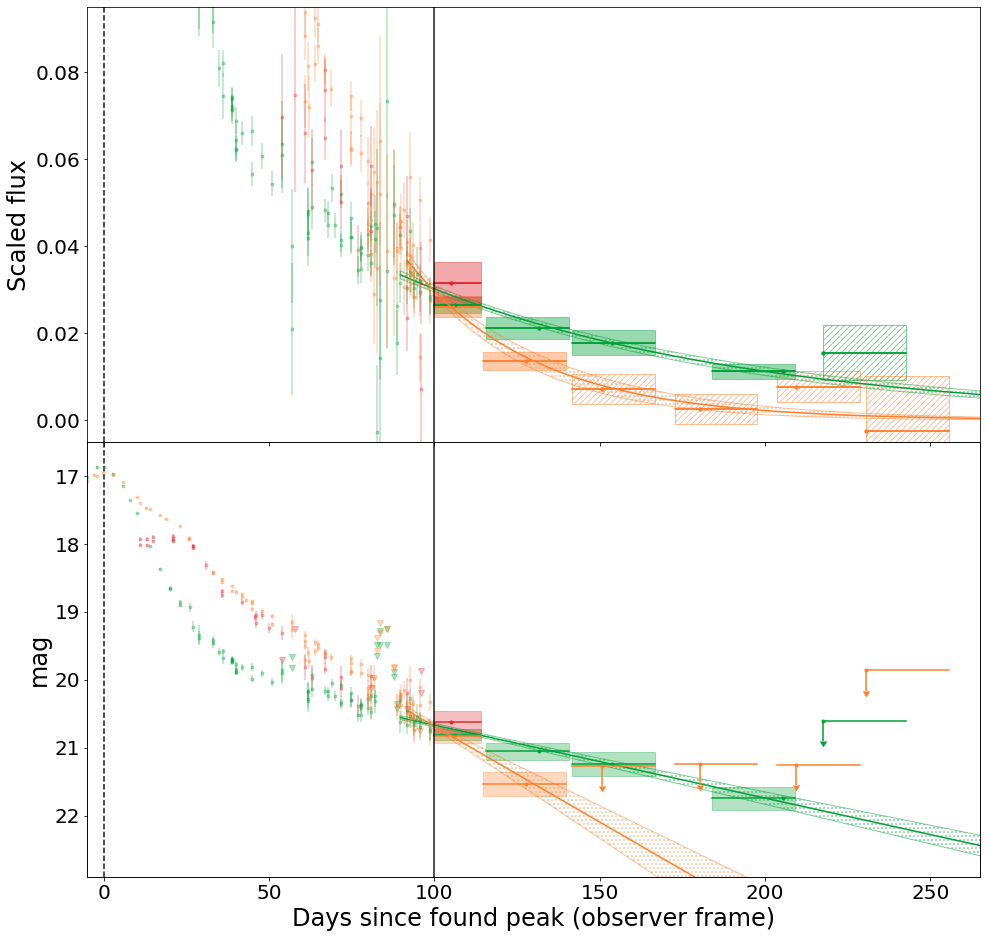
\includegraphics[width=\textwidth]{../Images/chapter_3/bin_showcase.png}
 \caption{First 250 days of the \ztfg\ztfr\ztfi-band light curves of SN 2019hbb in flux scaled to the peak flux (top panel) and magnitude (bottom panel) space. Binning starts 100 days after the estimated peak date (vertical black dashed and solid lines), using 25\,d bins. The $g$-, $r$-, and $i$-bands are shown green, orange, and red, respectively. Before 100 days, we show the unbinned detections with their uncertainties (coloured circles) and non-detections (inverted triangles). After 100 days we show the bins as horizontal lines to show their size, a circle to show their mean value, and the shaded region showing the 1$\sigma$ uncertainty (dashed regions are non-detections). A bin is deemed a non-detection if the flux $f<5\sigma_f$. The $5\sigma$ magnitude limit is calculated and shown as a downward arrow. In both the $g$- and $r$-bands, the first bin is a detection and there are multiple adjacent bins with detections, triggering the tail-fitting procedure (see Section \ref{tail_removal}). The resulting tail fits are shown in the green and red lines, respectively, with their 1$\sigma$ uncertainties as hashed regions. The half-life times are $t_{1/2,g} = 70 \pm 6$\,d ($\chi^2_\text{red} = 0.6$) and $t_{1/2,r} = 27 \pm 4$\,d ($\chi^2_\text{red} = 1.4$). This tail is therefore deemed to be a normal SN Ia tail.}
 \label{bin_showcase}
\end{figure}

\subsection{Removal of SN Ia radioactive tail detections}
\label{tail_removal} 
For some nearby SNe Ia, the normal light curve tail powered by the radioactive decay of $^{56}$Co $\rightarrow$ $^{56}$Fe is still visible at the phases investigated here ($>$100 d after the peak), possibly triggering false positives in our pipeline. To test if the fading tail is the reason for detections after 100 d, we checked if the detections follow a declining power law in flux space consistent with that of a normal SN Ia tail. We take all bins, normalise to the brightest data point, and fit a declining power law. To ensure that the tail matches the earlier data points, we include the unbinned observations between 60 and 100 d after the peak, making sure that if there are N bins only the latest N/2 unbinned detections are used to ensure that the fit focusses on the bins and not the unbinned points.

A successful fit of a declining normal SN Ia tail has a reduced chi-square of $\chi^2_\text{red, fit} < 5$ and fitted half-life of $t_{1/2}$ with uncertainty $\sigma_{t1/2}$, satisfying $t_{1/2} - 5\sigma_{t1/2} \leq 50$ d. We chose a threshold of 50\,d as \citealt{Georgios_11fe} showed that this is the approximate decay time scale for a normal SN Ia at these phases. A fit with a high $\chi^2_\text{red, fit}$ value could have failed due to bad or uncertain data, or due to the late-time detections not following a power law decay. Fits with a $t_{1/2}$ significantly larger than that of a normal SN Ia tail suggest an additional luminosity source contributing to the light curve at these phases. Figure~\ref{bin_showcase} shows an example where this tail fitting procedure determines the late-time detections in an object to be a normal declining SN Ia tail. 432 SNe Ia that were flagged as having late-time detection are discounted from further discussion because their light curves can be explained by a normal fading SN Ia tail. 


\subsection{SuperNova Animation Programme (SNAP)}
\label{snap}
 After performing the binning and filtering, and removing SNe Ia with contamination from the radioactive tail, we are left with 134 SNe Ia with robust late-time detections (see Table \ref{obj_breakdown}). Since the binning and filtering programme is designed to handle a large quantity of light curves and cannot be tailored specifically to suit the peculiarities of a single object, it is possible that there are objects remaining with issues in the data or data processing (e.g.~cosmic rays, bad subtractions), resulting in false positive detections. Therefore, we manually check the difference imaging to search for potential issues. To do this efficiently, we use \textsc{snap}\footnote{\url{https://github.com/JTerwel/SuperNova_Animation_Program}}.

Using \textsc{ztfquery} \citep{ZTFquery}, \textsc{snap} takes all difference images of the requested sky position during the requested time period(s) in the requested band(s) and shows them in chronological order in an animation. At the start of each animation the reference images in all bands are shown. The programme can show the image in grey-scale, a three-dimensional wire-frame representation of the intensities measured per pixel, the averaged values along both axes of the image, the observation date and duration, the peak and mean pixel values of the shown region, the last spectrum taken before the currently shown image, and highlight the resulting forced photometry point in the light curve corresponding to the plotted images.

Using \textsc{snap}, issues in the difference images can be identified, including SN ghosts (the SN is visible in the reference image, leaving a negative imprint in difference images after it has faded), cosmic rays, and bad pixels (NaN, or a large negative number). Variability of a separate source can also be seen, which, when close by, can contaminate the forced photometry at the SN location, for example, an active galactic nucleus (AGN).


\subsection{Simulated interaction recovery fractions}
\label{simulation}
To make sure the binning programme works as expected and estimate its detection efficiency in finding late-time signals, we simulated an observing campaign using \textsc{simsurvey} \citep{simsurvey, simsurvey_main}, a python package designed to simulate large scale time domain surveys such as ZTF. To successfully simulate an observing campaign, the programme needs to be told what, when, where, and how something is observed, and under what conditions. For this, we need a model of the SN Ia-CSM that is going to be observed, an explosion rate as a function of redshift, and a time range for these explosions to occur. We also require an observing log specifying which part of the sky is being observed at a specific time, the length of the observations, and the weather conditions during the observations. Lastly, we require details of the camera that is used to carry out the observations. The SN model needs to be in a similar format to the \textsc{sncosmo} models (a \textsc{python} package made for supernova cosmology, \citealt{sncosmo}). This means we need a set of spectra over the entire phase range, all having the same wavelength spacing and range. Since no such model exists, we built our own model as described in the next section.

\subsubsection{The interacting SN model}
\label{model_description}

We chose SN 2011fe as the template of a normal SN Ia as it is well observed and close by (in M101 at a distance of 6.4 Mpc, \citealt{M101_cep_dist}). Optical spectra of SN 2011fe were obtained between phases of $-$18 to 1017\,d relative to the peak. We made a custom model using \textsc{sncosmo} and spectra found on WISeREP \citep{wiserep}\footnote{\url{https://wiserep.weizmann.ac.il}}, which are listed in Table \ref{11fe_sources}. The spectra were flux calibrated to match the observed coeval broadband magnitudes. Spectra up to 45\,d after the peak were flux calibrated using a \textsc{salt2} \citep{salt2} fit of the \textit{PTF48g} and \textit{PTF48R}-band photometry \citep{PTF_1, PTF_2}, which is used to estimate the flux in the $g$- and $r$- bands at these phases. Spectra between 45 and 400\,d are flux calibrated using a cubic spline interpolation of photometry in the \textit{PTF48g}- and \textit{PTF48R}-bands. The interpolation extends up to 600\,d after the peak in the \textit{PTF48R}-band, there is no \textit{PTF48g} photometry used between 400 and 600\,d after the peak. Three interpolated photometry points from the \textsc{salt2} fits were used as anchor points to connect these two parts of the calibration. \citet{Georgios_11fe} show that there is a slight kink in the light curve tail around 600\,d after the peak. This is replicated in the model by calibrating all spectra more than 600\,d after the peak using a cubic spline interpolation of photometry from the Large Binocular Telescope \citep[LBT;][]{LBT} in the Bessel \textit{R}-band \citep{Shappee_11fe}.

After flux calibration, the spectra were dereddened to remove dust extinction effects, using the \citet{ccm89_extinction_law} extinction law with $A_V = 0.04$ mag \citep{extinction_Av}. The spectra were rebinned, and any wavelength region that was not covered in all spectra was removed as required by \textsc{simsurvey}. Lastly, the model is corrected for distance, redshift and time dilation. The resulting model is that of a normal SN Ia, which exploded at a distance of 10 pc without any dust between the source and observer.

 The best late-time detection of CSM in a normal/91T-like SN Ia was for SN 2015cp, where \Halpha\ emission was identified in its spectra at 664 d after light-curve peak \citep{2015cp}. To model potential CSM interaction signals similar to that of SN 2015cp, we add a narrow \Halpha~line with a Gaussian profile to the SN 2011fe model. Due to the rareness of interaction in otherwise normal SNe Ia, we do not have good constraints on the diversity of interaction signatures and simulate a broad parameter space. The interaction was chosen to start at 100, 200, 300, or 500 days after the peak, last for 100, 300, or 500 days, and have a similar brightness to the observed signal in SN 2015cp \citep{2015cp}, as well as 10 times weaker or 10 times stronger than it. All possible combinations of these values are used, and a simulation without any interaction is also used as a control test, giving a total of 37 simulations. 

Figure~\ref{mod_15cp_comp} shows an example of our model spectra at 300\,d and SN 2015cp at 694\,d in the rest frame \citep{2015cp}. It also shows the model redshifted to $z = 0.07$, where the \Halpha~line is partly shifted into the \ztfi-band. Figure~\ref{11fe_mods} shows the absolute magnitude \ztfr\ztfi-band light curves of the SN 2011fe model in the rest frame, as well as light curves with different strengths of \Halpha~emission. Our interaction model will only generate a late-time interaction signal in the \ztfr-band (or \ztfi-band at $z > 0.06$) as we only add a \Halpha\ emission line. This is enough to test the binning programme but is likely too simple to reflect the actual late-time signal seen in SN 2015cp (which also showed \OI\ and \CaII\ in the restframe \ztfi-band) or potential other events.


\begin{figure}
 \centering
 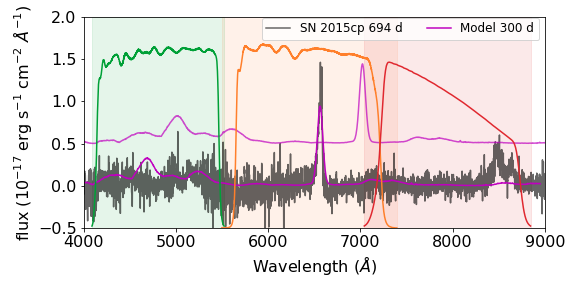
\includegraphics[width=\textwidth]{../Images/chapter_3/Model_15cp_comparison.png}
 \caption{Model spectrum at 300 days (SN 2011fe with the added \Halpha~line) is shown in magenta overlaid on a rest-frame spectrum of SN 2015cp at 694 days in grey. The model flux has been scaled to the distance of SN 2015cp for comparison. The green, orange, and red shaded regions are the bandwidths of the \ztfg-, \ztfr-, and \ztfi-bands, respectively. The transmission profiles are plotted in the same colours for each band. The model is also shown shifted to $z = 0.07$ (and offset up in flux), where the \Halpha~line has just started to be in the \ztfi-band.}
 \label{mod_15cp_comp}
\end{figure}

\begin{figure}
 \centering
 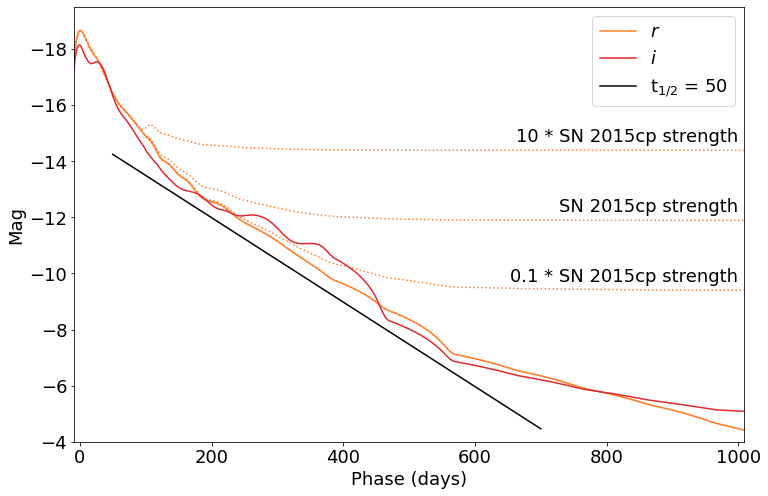
\includegraphics[width=\textwidth]{../Images/chapter_3/11fe_mods.png}
 \caption{\ztfr (orange) and \ztfi (red) absolute magnitude light curves of the SN 2011fe model used in the simulations in the ZTF bands as a function of phase from rest-frame \textit{B}-band peak \citep{spec_HST}. The bumpiness in the models is because the underlying \textsc{sncosmo} model class interpolates in flux space but fails to find an exponential decay. The added rest-frame CSM interaction model based on \Halpha~emission (starting at a phase of 100 d) is shown with dotted lines for the \ztfr-band. Once the interaction becomes the dominant source, it smooths out the bumps from the underlying tail. The black line shows a radioactive decay with t$_{1/2}=50$ d, typical of a declining normal SN Ia tail.}
 \label{11fe_mods}
\end{figure}

\subsubsection{Simulating the observing campaign}
\label{sim_obs}
By specifying the object to observe, as well as the telescope details and observation schedule, an observation campaign can be performed using \textsc{simsurvey} resulting in a collection of observed light curves. For a deeper explanation of \textsc{simsurvey} we refer the reader to \cite{simsurvey_main}. The parameters used as input are listed in Appendix \ref{sec:simsurvey_inputs}. In each \textsc{simsurvey} run, $10^5$ SNe Ia are simulated to produce observed light curves and meta-data such as redshift, observed peak date, etc. To ensure that the SNe Ia are similar around the peak to those recovered, we require that the SN Ia light curves must have at least three detections of $\geq$5$\sigma$ and are brighter that 19 magnitude at the peak. This reduces the sample to $\sim$ 40,000 objects per simulation. These are sent through the binning and filtering programme (Section \ref{pipeline}) as if they were real observed light curves to determine the recovery efficiency. 

The volumetric rate used as input in the simulations favours more distant SNe, which results in very few SNe at extremely low redshift values and hence larger uncertainties. To mitigate this, we split $0\leq z\leq 0.015$ into bins of size 0.001 and simulate an additional 100 SNe in each bin using the same parameters as in the original simulations. Introducing these additional events does not impact the recovery efficiencies because we are comparing the number of recovered events relative to the input number in each redshift bin and therefore, are insensitive to the input rate of events. 


\subsubsection{Simulated interaction recovery}
\label{simulated_reco}
Our aim is to determine from our simulations how many SNe Ia with signatures of late-time interaction similar to that of SN 2015cp would have been detected by our pipeline. For each of the simulations, we binned the SNe based on their redshift and looked at the fraction of SNe that were reported by the pipeline to show late-time excesses. Figure~\ref{recov_fracs} shows the recovery fractions as a function of redshift for an example simulation when the interaction starts at 500\,d and lasts for 500 d for simulations of no CSM interaction, late-time interaction with the same strength as SN 2015cp, and interaction 10 times as strong as SN 2015cp (strong interaction). As expected the recovery fraction drops off with increasing redshift for both the SN 2015cp equivalent strength and the interaction that is 10 times stronger, with the strong interaction recoverable out to a higher redshift. 

The recovery fraction of the simulations with CSM interaction does not reach 100 per cent in the lowest redshift bins. This is because the radioactive tails of these SNe Ia tend to be bright out to hundreds of days after explosion. Therefore, depending on the cadence and uncertainties of the simulated photometry, the SN light can dominate over the CSM interaction and the CSM interaction signal does not alter the shape of the SN decay tail enough to be flagged as CSM interaction. 

In the simulation without CSM interaction, the recovery fraction is non-zero at small redshifts, meaning that some objects are falsely identified as having late-time excess. For these very bright and high signal-to-noise SN Ia light curves, our decaying tail model for normal SNe Ia proves to be too simple. Our analysis pipeline detects real deviations of the SN light curve evolution from our simple decay tail model. This only occurs at the lowest redshifts and nearby SNe Ia are rare, with only 0.6\% of our observed SN Ia sample at $z\leq0.01$. This means that contamination of our sample due to normal SNe Ia tails that cannot be fit by our simplified tail fit model is very low. 

We fitted a sigmoid function to the recovery fractions of each simulation, using the total amount of objects in each bin as its weight (Fig.~\ref{recov_fracs}). A sigmoid function is an oversimplification (the recovery fraction is underestimated at the low redshifts) but it allows us to easily estimate the redshift limit where CSM interaction can be recovered. We define our redshift limit where CSM interaction can be recovered as $z_{50}$, the redshift where 50 per cent of the SN interactions are recovered. These values are listed for all simulations in Table \ref{sim_z50_results}.


\begin{figure}
 \centering
 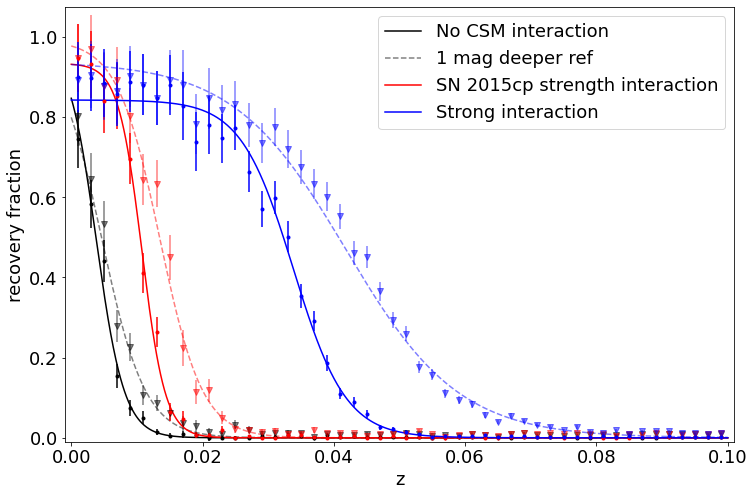
\includegraphics[width=\textwidth]{../Images/chapter_3/recov_fracs.png}
 \caption{Fraction of SNe Ia for one of our simulations (interaction occurring between 500 -- 1000\,d after the peak) where the CSM interaction was recovered per redshift bin of size $0.002$. The simulations are shown for interaction strengths of zero (grey), similar to SN 2015cp (red), and 10 times stronger than SN 2015cp (blue). In the simulation without CSM interaction, the recovery fraction should be interpreted as the fraction of false positives. The simulations with normal ZTF quality reference images are shown with dots and fitted sigmoid functions with solid lines. Simulations where one magnitude deeper reference images were assumed are shown in triangles, with their fitted sigmoid functions in dashed lines.}
 \label{recov_fracs}
\end{figure}

 As discussed in Section \ref{model_description}, we simulated 36 models with interaction signatures starting at 100, 200, 300 and 500 d post peak, lasting for 100, 300 and 500 d, and with strengths the same as SN 2015cp, 10 times weaker and 10 times stronger. We also simulated a model without any late-time CSM interaction. For the models with an interaction strength similar to SN 2015cp \citep{2015cp}, when the interaction is short and early (starting 100 days after the peak and lasting for 100 days), the interaction cannot be distinguished from a normal SN Ia decaying light curve and the recovery fraction is as low as the no interaction simulation. When the interaction is longer, or if it starts later, the light curve flattens enough to be identified as deviating from a normally declining SN Ia tail. This pushes the redshift boundary where 50 per cent of the interaction would be recovered by ZTF to $z_{50} = 0.0105 \pm 0.0003$ for the longest and latest interaction (500 - 1000 days after peak).

If the CSM interaction is 10 times weaker than that of SN 2015cp, the decaying SN Ia tail generally dominates over the interaction signature and the light curve shows little deviation from a normal decaying SN Ia tail. Even in the best case scenario of the longest and latest CSM interaction simulation, the 50 per cent recovery thresholds lies at $z_{50} = 0.0050 \pm 0.0005$. In the simulations where the interaction is 10 times stronger compared than that of SN 2015cp, the shortest and earliest interaction (lasting from 100 to 200 days after peak) has $z_{50} = 0.0091 \pm 0.0014$. For the longest and latest interaction, the 50 per cent recovery rate is at $z_{50} = 0.0323 \pm 0.0004$.


\subsubsection{Impact of reference image depth}
\label{impact_refdepth}
The mean limiting magnitude of the ZTF reference images is $\sim 21.8$ mag and as discussed in \citep{ref_uncert}, this is the limiting factor for recovering faint signals from binned light curve data. To test the improvement of deeper reference images, the assumed limiting magnitude was changed to be 0.5 and 1 mag deeper. The recovery fraction for one magnitude deeper is shown for comparison in Fig.~\ref{recov_fracs}. As expected, deeper reference images allows the interaction signatures to be detected to higher redshift, although the increases in $z_{50}$ values are modest (see Table \ref{sim_z50_results}). For example, for the latest onset and longest interaction duration interaction, $z_{50}$ increases from $0.0323 \pm 0.0004$ to $0.0407 \pm 0.0009$.


\section{Results}
\label{results}

We run our custom detection pipeline on the ZTF DR2 light curves in the same way as it was performed on the simulated light curves in Section \ref{simulation}. In 1932 light curves, nothing is detected in any of the 16 trials discussed in Section \ref{pipeline}, in 432 light curves the late-time detections are attributed to declining SN Ia tails, and in 1020 light curves the detections were not considered robust (<4 successful trials). These are the three largest cuts in our sample, as can be seen in Table\,\ref{obj_breakdown}, and leave us with 134 light curves that pass the pipeline. In Section\,\ref{results_summary}, we describe the light curves of these events and discuss how some light curves fit into known classes of events (e.g. known Ia-CSM, late-time SN Ia tail detections). In Section \ref{Additional_tests}, we describe the additional tests that were performed on the remaining promising 10 events to determine if their late-time excesses are due to CSM interaction or other scenarios. 


\subsection{Initial summary of detected events}
\label{results_summary}

As can be seen in Table \ref{obj_breakdown}, the result of the pipeline is a list of 134 objects that require visual inspection after passing the detection cuts of positive $>$5$\sigma$ detections in adjacent light curve bins in at least four of the 16 bin size and placement combinations. In 47 of these cases, by visual inspection we identify that an incorrect baseline caused false positives. In five cases, the peak date estimation failed and estimated the peak to be over 100 days before the actual SN explosion. Because of this the SN itself was detected as a late-time signal. Furthermore, in 29 cases there was evidence of the host galaxy being improperly subtracted or showing signs of activity, which interfered with the forced photometry at the SN location. Finally, in 20 cases the tail fit test was unable to show the nature of the tails due to various reasons (e.g. the fits did not converge properly or there was a gap in the observations while the tail was visible). After this step, 33 objects were remaining in the sample.

 %\begin{landscape}
  \begin{table}
   \centering
   \caption{List of objects that passed the initial visual inspections.}
   \resizebox{\textwidth}{!}{%Scale table to page width
   \begin{tabular}{llccccccccccccc}
    \hline
    Name & IAU name & Redshift & Type $^{(a)}$ & Peak & Peak & Excess & Excess & Excess & Group $^{(b)}$ \\
    &&&& MJD & mag.& phase (d) & band & mag. \\
    \hline
    ZTF18aaykjei  & SN 2018crl & 0.09690 $\pm$ 0.00002 & Ia-CSM & 58297.3 & 18.40 $\pm$ 0.04  & 100 -- 400 & \ztfr & 20.1 -- 21.9 & Known Ia-CSM \\
    ZTF18abuatfp  & SN 2018gkx & 0.13643 $\pm$ 0.00001 & Ia-CSM & 58382.1 & 18.71 $\pm$ 0.05  & 100 -- 475 & \ztfg\ztfr\ztfi & 19.6 -- 21.5 & Known Ia-CSM \\
    ZTF18actuhrs  & SN 2018evt & 0.02442 $\pm$ 0.00001 & Ia-CSM & 58476.5 & 16.19 $\pm$ 0.01 & 100 -- 525 & \ztfg\ztfr\ztfi & 16.6 -- 21.8 & Known Ia-CSM \\
    ZTF19aaeoqst  & SN 2019agi & 0.05958 $\pm$ 0.00001 & Ia-CSM & 58511.5 & 18.46 $\pm$ 0.04  & 100 -- 450 & \ztfg\ztfr\ztfi & 19.2 -- 21.9 & Known Ia-CSM \\
    ZTF19abidbqp  & SN 2019ibk & 0.04014 $\pm$ 0.00001 & Ia-CSM & 58688.5 & 18.56 $\pm$ 0.05  & 100 -- 1125 & \ztfg\ztfr & 19.1 -- 21.5 & Known Ia-CSM \\
    ZTF19acbjddp  & SN 2019rvb & 0.1832 $\pm$ 0.0004 & Ia-CSM & 58790.1 & 18.90 $\pm$ 0.06  & 100 -- 400 & \ztfg\ztfr & 20.4 -- 22.0 & Known Ia-CSM \\
    ZTF20aatxryt  & SN 2020eyj & 0.0294 $\pm$ 0.0004 & Ia-CSM & 58939.2 & 17.24 $\pm$ 0.01 & 100 -- 450 & \ztfg\ztfr & 19.0 -- 21.8 & Known Ia-CSM \\
    ZTF20abbbsfs  & SN 2020kre & 0.13530 $\pm$ 0.00001 & Ia-CSM & 58998.2 & 19.09 $\pm$ 0.04  & 175 -- 425 & \ztfg\ztfr & 19.8 -- 21.4 & Known Ia-CSM \\
    ZTF20abmlxrx  & SN 2020onv & 0.0940 $\pm$ 0.0004 & Ia-CSM & 59052.4 & 17.85 $\pm$ 0.01  & 100 -- 500 & \ztfg\ztfr & 18.8 -- 21.6 & Known Ia-CSM \\
    ZTF20abqkbfx  & SN 2020qxz & 0.0968 $\pm$ 0.0004 & Ia-CSM & 59094.3 & 18.18 $\pm$ 0.04  & 100 -- 450 & \ztfg\ztfr\ztfi & 19.5 -- 21.9 & Known Ia-CSM \\
    ZTF20accmutv  & SN 2020uem & 0.043 $\pm$ 0.001  & Ia-CSM & 59173.5 & 16.38 $\pm$ 0.01 & 100 -- 525 & \ztfg\ztfr & 17.4 -- 21.4 & Known Ia-CSM \\
    ZTF20aciwcuz  & SN 2020xtg & 0.06122 $\pm$ 0.00001 & Ia-CSM & 59189.5 & 17.45 $\pm$ 0.02  & 100 -- 500 & \ztfg\ztfr\ztfi & 18.0 -- 21.9 & Known Ia-CSM \\
    ZTF20acyroke  & SN 2020aeuh & 0.12665 $\pm$ 0.00004  & Ia-CSM & 59217.4 & 19.01 $\pm$ 0.06 & 100 -- 250 & \ztfr & 19.8 -- 20.9 & Known Ia-CSM \\
    \hline
    ZTF18aasdted  & SN 2018big & 0.01814 $\pm$ 0.00001 & Ia-norm & 58268.4 & 15.64 $\pm$ 0.01 & 450 -- 550 & \ztfg\ztfr & 20.4 -- 21.5 & Sibling  \\
    ZTF19aaysiwt  & SN 2019hnt & 0.0926 $\pm$ 0.0004 & Ia  & 58651.2 & 18.46 $\pm$ 0.05  & 525 -- 625 & \ztfg\ztfr & 20.5 -- 21.7 & Sibling  \\
    ZTF19acihfxz  & SN 2019tjz & 0.055 $\pm$ 0.003  & Ia-norm & 58795.1 & 18.00 $\pm$ 0.03  & 950 - 1050 & \ztfr & 19.4 -- 20.7 & Sibling  \\
    ZTF20abzetdf  & SN 2020tft & 0.071 $\pm$ 0.002  & Ia-norm & 59113.5 & 18.2 $\pm$ 0.1  & 725 -- 800 & \ztfr & 19.4 -- 20.2 & Sibling  \\
    ZTF20acehyxd  & SN 2020uvd & 0.0346 $\pm$ 0.0005 & Ia-norm  & 59129.3 & 18.72 $\pm$ 0.03  & 300 -- 350 & \ztfr & 20.2 -- 21.5 & Sibling  \\
    \hline
    ZTF19aatlmbo  & SN 2019ein & 0.0072 $\pm$ 0.0001  & Ia-norm & 58617.2 & blinded $^{(c)}$    & 100 -- 425 & \ztfr & 18.9 -- 21.8 & Kinked tail \\
    ZTF20abqvsik  & SN 2020rcq & 0.00246 $\pm$ 0.00001 & Ia-norm & 59144.5 & blinded $^{(c)}$    & 100 -- 400 & \ztfi & 16.5 -- 22.2 & Kinked tail \\
    ZTF20abrjmgi  & SN 2020qxp & 0.00356 $\pm$ 0.00001 & Ia-91bg & 59088.1 & blinded $^{(c)}$    & 100 -- 375 & \ztfr & 17.9 -- 21.8 & Kinked tail \\
    ZTF20abwrcmq  & SN 2020sck & 0.01643 $\pm$ 0.00001 & Iax & 59099.4 & 16.25 $\pm$ 0.01 & 100 -- 450 & \ztfg\ztfr\ztfi & 19.1 -- 21.9 & Kinked tail \\
    ZTF20achlced  & SN 2020uxz & 0.00867 $\pm$ 0.00008 & Ia-norm & 59142.4 & blinded $^{(c)}$    & 100 -- 400 & \ztfg\ztfr & 17.1 -- 21.9 & Kinked tail \\
    \hline
    ZTF19acwrqtv  & SN 2019vzf & 0.059 $\pm$ 0.004  & Ia-99aa  & 58829.1 & 18.00 $\pm$ 0.07  & 150 -- 400 & \ztfg\ztfr & 20.7 -- 21.8 & Other -- AGN $^{(d)}$   \\ 
    ZTF20aahptds  & SN 2020awr & 0.07649 $\pm$ 0.00002 & Ia-norm & 58888.5 & 18.54 $\pm$ 0.07 & 300 -- 1050 & \ztfi & 20.2 -- 20.5 & Other -- data issue $^{(d)}$  \\
    ZTF20aazwuin  & SN 2020kzd & 0.082 $\pm$ 0.001  & Ia-norm & 58997.4 & 18.86 $\pm$ 0.03  & 250 -- 850 & \ztfg\ztfr & 21.3 -- 22.0 & Other -- data issue $^{(d)}$  \\
   \hline 
    ZTF18abtqevs$^*$ & SN 2018grt & 0.042 $\pm$ 0.003  & Ia-norm & 58372.3 & 18.56 $\pm$ 0.02 & 1350 -- 1450 & \ztfr & 21.1 -- 21.3 & Other   \\
    ZTF19aanyuyh  & SN 2020pkj & 0.02456 $\pm$ 0.00001 & Ia-norm & 59060.4 & 16.90 $\pm$ 0.01& 100 -- 175 & \ztfr & 20.8 -- 21.1 & Other   \\
    ZTF19abfvhlx$^*$ & SN 2019ldf & 0.05646 $\pm$ 0.00001  & Ia-norm & 58686.5 & 17.90 $\pm$ 0.04 & 1050 -- 1225 & \ztfr\ztfi & 20.1 -- 21.1 & Other   \\
    ZTF19ablekwo  & SN 2019mse & 0.088 $\pm$ 0.004  & Ia-norm & 58715.4 & 18.37 $\pm$ 0.02 & 450 -- 700 & \ztfg\ztfr\ztfi & 19.8 -- 20.6 & Other   \\
    ZTF19abzwtiu  & SN 2019rqn & 0.075 $\pm$ 0.003  & Ia-norm & 58760.3 & 18.62 $\pm$ 0.03 & 950 -- 1050 & \ztfi & 20.6 -- 21.4 & Other   \\
    ZTF20aaifyfx  & SN 2020alm & 0.06001 $\pm$ 0.00001 & Ia-norm  & 58873.5 & 18.10 $\pm$ 0.02 & 750 -- 1025 & \ztfg\ztfr\ztfi & 19.9 -- 21.9 & Other   \\
    ZTF20abjfufv$^*$ & SN 2020tfc & 0.031 $\pm$ 0.001  & Ia-norm & 59116.3 & 17.22 $\pm$ 0.01& 550 -- 800 & \ztfg\ztfr\ztfi & 18.9 -- 21.4 & Other   \\
    \hline
  \end{tabular}
  }
  \label{33_list}
  \begin{flushleft}
  *Our three final objects with suggested detections of late-time interaction. \\
  $^{(a)}$Type is based on spectral classifications (Rigault et al.,~in prep.), Ia-CSM are those interacting with CSM that is observed around peak, Ia-norm are those that are most consistent with a normal SN Ia, Ia are those without a sub-classification but are consistent with being a SN Ia, and SN 2020sck is a Iax \citep{2020sck_Iax}.\\
  $^{(b)}$The objects are split into four groups: Ia-CSM that were previously known, identified siblings, SNe Ia that are detected due to their early-time tail fits showing a kink (Kinked tail), and the `Other' category that includes ten events with potential flux excesses, including three (SN 2019vzf, SN 2020awr and SN 2020kzd) that are subsequently ruled out (see Section \ref{Additional_tests}). \\
  $^{(c)}$The peak magnitudes of four SNe Ia in the sample are blinded because of their planned use in H$_0$ constraints (Rigualt et al.,~in prep.).\\
  $^{(d)}$SN 2019vzf is ruled out as a true excess due to AGN variability at the position, in SN 2020awr the excess is only detected in the \ztfi and is ruled out by the scene modelling analysis, and SN 2020kzd is detected in the \ztfg\ztfr bands on a complex galaxy environment and not detected in the scene modelling analysis (see Section \ref{sec:scene_modelling}). 
  \end{flushleft}
 \end{table}
%\end{landscape}


Further details of these remaining 33 SNe Ia are shown in Table \ref{33_list} and can be split up into four main groups: i) known Ia-CSM events, ii) transient siblings, where a second transient event occurs near the identified SN Ia causing its light to (partially) be picked up during forced photometry at the first SN location, iii) nearby objects whose tail could not be fitted by our simple model, and iv) objects that do not fall in the first three groups. In the following sections, we describe the first three of these groups that are not due to potential CSM interaction at late times. 


\begin{figure*}
 \centering
 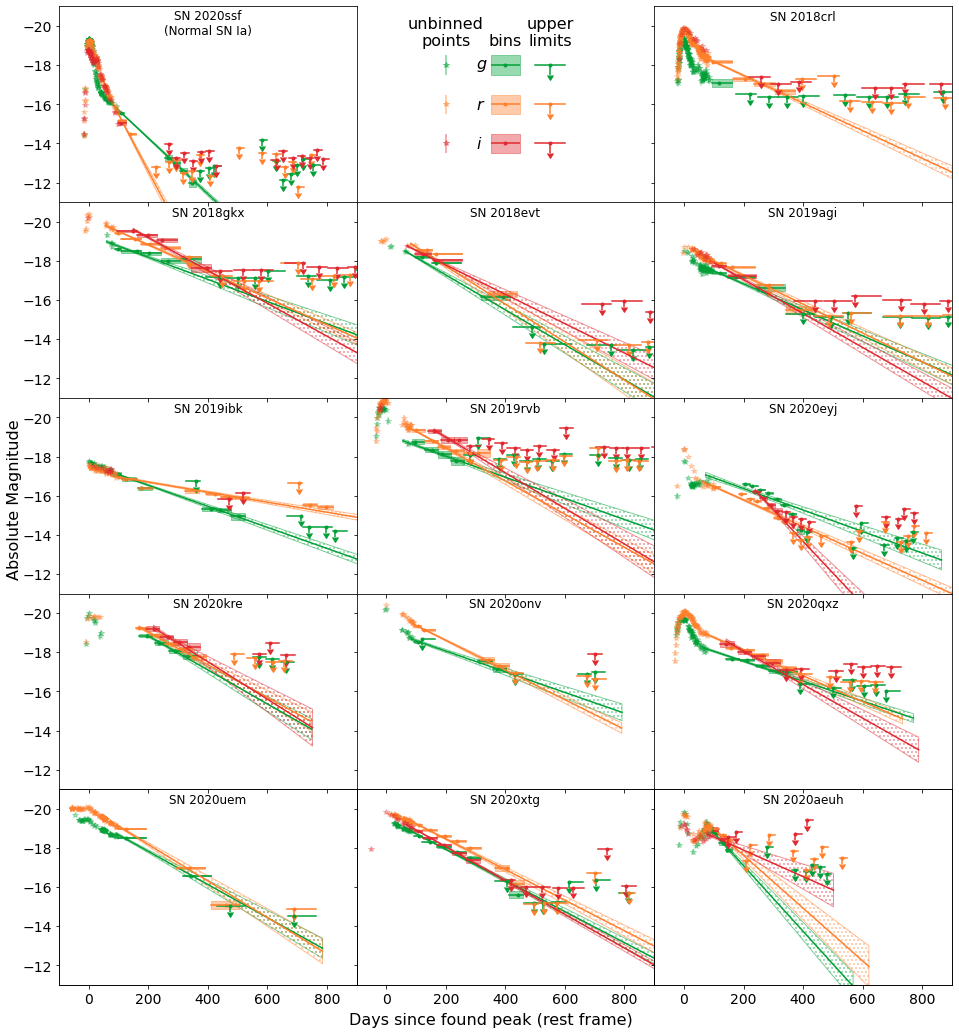
\includegraphics[width=\textwidth]{../Images/chapter_3/known_CSM_plots.png}
 \caption{Binned late-time observations of the recovered known SNe Ia-CSM. All objects are shown in absolute magnitude and over the same time range for easy comparison. All objects are detected beyond 100 days after the peak without using the binning technique. We do not show these individual data points to increase readability. The tail fits are shown as solid lines with the hashed region denoting their 1$\sigma$ uncertainties. For comparison, SN 2020ssf (ZTF20abyptpc) in the top left corner is a normal SN Ia with a normally declining tail with $t_{1/2,g} = 53 \pm 1$ days and $t_{1/2,r} = 26 \pm 1$ days. The fitted tails for the SNe Ia-CSM are significantly shallower.}
 \label{known_CSM_plots}
\end{figure*}


\subsubsection{Known Ia-CSM}
\label{known-iacsm}
The first group are the 13 known Ia-CSM, defined as those objects that already had a Ia-CSM classification. These objects started interacting relatively soon after the explosion and remained active long enough to be picked up by our pipeline beyond the 100 day threshold. Figure~\ref{known_CSM_plots} shows the light curves of the recovered SNe Ia-CSM in absolute magnitude space (uncorrected for extinction). Even if the peak identified by our code is not the real peak due to it not being observed (e.g. for SN 2018evt, SN 2019agi, and SN 2019ibk), the CSM interaction persists for long enough for it to be picked up by our pipeline.

Ten of the known Ia-CSM SNe are presented in \citet{Ia-CSM_BTS}, who search for SNe Ia-CSM discovered in the ZTF Bright Transient Survey from May 2018 to May 2021 \cite[BTS;][]{BTS-I, BTS-II}. They find two objects that are not in our sample: SN 2020abfe (ZTF20acqikeh) and SN 2020aekp (ZTF21aaabwzx). SN 2020abfe is in the DR2 sample, but due to a combination of a gap in the observed light curve and the interaction not altering the declining tail sufficiently, our tail fit procedure is unable to distinguish it from a normal declining SN Ia tail. SN 2020aekp was first detected after the final date for objects to be included into our sample. Two of the events in our sample (SN 2020eyj and SN 2020kre) are not presented in \citet{Ia-CSM_BTS}. SN 2020eyj was excluded as \citet{Ia-CSM_BTS} focussed on interaction with H-rich material and this object showed He emission lines suggesting interaction with He-rich material \citep{Kool_He_CSM}. SN 2020kre is not in the BTS sample and therefore, not included in \cite{Ia-CSM_BTS}. However, it was confirmed with spectroscopy to have \Halpha~emission in its peak spectra.

Out of the 13 events SN 2020aeuh is an outlier, due to its distinct light curve. While the other 12 known Ia-CSM events detected in our sample have decline tails whose slopes are significantly shallower than for a normal SN Ia or steepen over time, SN 2020aeuh brightens significantly, having a double peaked nature with the second peak at around 100\,d after the first. Even though the light curve suggests the SN to be interacting, no H emission (\Halpha~or other lines) are observed. Kool et al.~(in prep) present a detailed analysis of this object. 


\subsubsection{Siblings}

\begin{figure*}
 \centering
 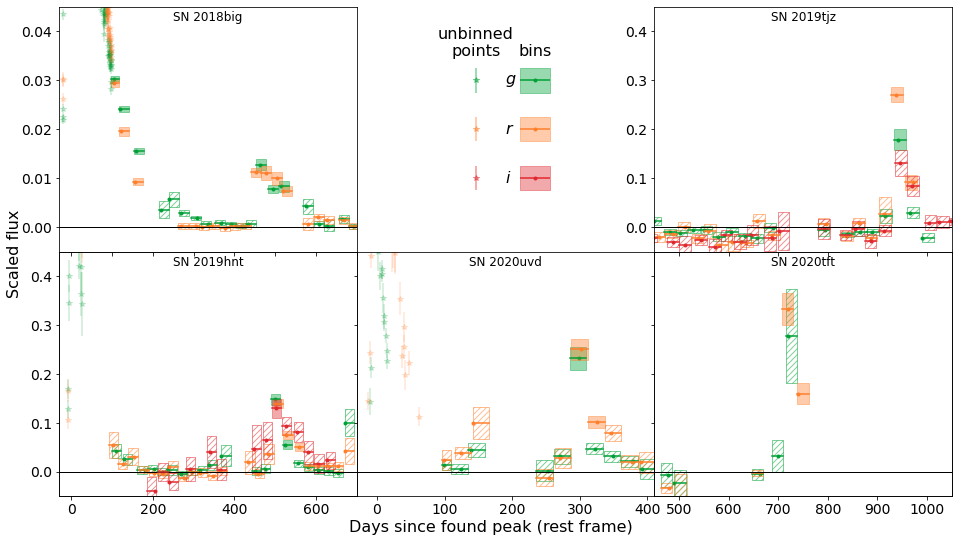
\includegraphics[width=\textwidth]{../Images/chapter_3/sibling_norm_plots.png}
 \caption{Binned late-time observations in flux space of the five events with a detected sibling, with the flux normalised to the found peak flux. All objects are plotted on the same flux scale for easy comparison except for SN 2018big, as its late-time detections are much weaker compared to the original SN peak magnitude due to the larger distance offset between the siblings.}
 \label{sibling_plots}
\end{figure*}

\begin{figure}
 \centering
 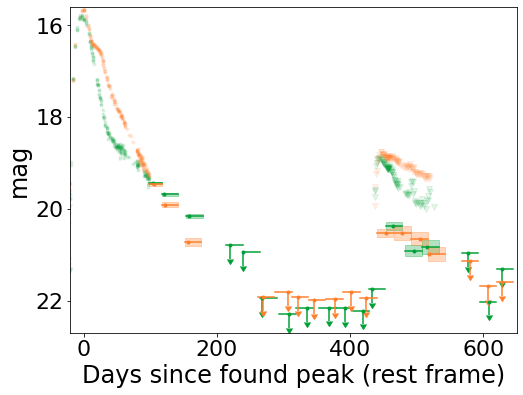
\includegraphics[width=\textwidth]{../Images/chapter_3/ted.png}
 \caption{Light curves of SN 2018big and its sibling SN 2019nvm in magnitude space using bins of 25 d. The \ztfg (green) and \ztfr (orange) bins follow the tail of SN 2018big until it disappears in the noise. About 450\,d after the peak of SN 2018big, new detections are identified in the binned photometry. The individual observations remain upper limits, although their shape hint to the true nature of these late-time detections.}
 \label{sibling_example}
\end{figure}


\begin{table*}
 \centering
 \caption{Objects with a detected sibling transient.}
 \resizebox{\textwidth}{!}{%Scale table to page width
 \begin{tabular}{llllcccc}
  \hline
  Primary name & IAU name & Sibling name & IAU name$^b$ & Type & Date$^a$ & Offset ($\arcsec$)$^c$\\
  \hline
  ZTF18aasdted & SN 2018big & ZTF19abqhobb & SN 2019nvm & IIP & 58\,714 & 3.7\\
  ZTF19aaysiwt & SN 2019hnt & ZTF20acwpads & - & - & 59\,186 & 1.2\\
  ZTF19acihfxz & SN 2019tjz & ZTF18aanhpii & - & - & 59\,774 & 1.2\\
  ZTF20abzetdf & SN 2020tft & - & - & Ia & 59\,867 & $<$ 1\\
  ZTF20acehyxd & SN 2020uvd & ZTF21abouuow & SN 2021udv & Ia & 59\,422 & 3.1\\
  \hline
 \end{tabular}
 }
 \begin{flushleft}
$^a$MJD of the first detection of the sibling. \\
$^b$The siblings ZTF19aaysiwt and ZTF20acwpads share an IAU name. For ZTF20abzetdf, the siblings are too close together ($<$1$\arcsec$ separation) to be automatically recognised as separate events, causing them to share both ZTF and IAU names. ZTF18aanhpii is a sibling transient in 2022 on top of the host nucleus, resulting in the internal name being from 2018. \\
$^c$Angular separation on the sky between the siblings. \\
\end{flushleft} 
 \label{siblings}
\end{table*}


Siblings are transients that occur in the same host galaxy as each other and can be useful for understanding differences in local environments \citep[e.g.][]{biswas_siblings, ZTF_siblings}. In some cases, the siblings occur in (almost) the same place on the sky, only differing in explosion time. This can be either due to the two transients being physically close together, or a projection effect due to the inclination of the host. However, the result is the same: forced photometry at the location of one sibling will result in a (partial) recovery of the other. Assuming that the first transient is a SN Ia in our sample and the second transient is fainter, our pipeline will flag the late-time rebrightening as a late-time excess in one of our objects.

Careful examination of the images using \textsc{snap} and cross-referencing using Fritz (an alert broker, \citealt{skyportal2019, duev2019realbogus, Kasliwal_Growth, Skyportal}) and the Transient Name Server\footnote{https://www.wis-tns.org/} (TNS) showed that there are five objects in our shortlist whose late-time detections are due to a sibling. Figure~\ref{sibling_plots} shows the binned light curves of these objects in flux space. In each light curve there is a sudden significant spike in the detected fluxes in all observed bands, which falls back down again after a short period of time. Table \ref{siblings} lists the name and type of each sibling if known, as well as their sky separation. In some cases the siblings are close enough together that they are not automatically recognised as separate events, resulting in them having the same name. In the case of SN 2019tzj the sibling (ZTF18aanhpii) exploded close to the nucleus, which had some spurious detections in 2018. This caused the sibling to have a 2018 ZTF name, although it exploded in 2022.

Figure~\ref{sibling_example} shows the detection of a sibling (SN 2019nvm) in the late-time light curve of SN 2018big in magnitude space. SN 2019nvm is slightly offset ($\sim4\arcsec$) from the location of the original SN. The photometry pipeline forces the point spread function (PSF) fit at the position of SN 2018big. As the position of SN 2019nvm is slightly offset, only some of the total flux of SN 2019vnm is captured in the fit. 
Besides these five siblings, we identified two other pairs of siblings with \textsc{snap}: SN 2019gcm and SN 2021fnj, and SN 2020jgs and SN 2021och. These siblings were too far apart to be picked up with the forced photometry (9.6 and 10.8$\arcsec$, respectively) but were found while inspecting using \textsc{snap}. For a complete list and study on the siblings found in the ZTF DR2, we refer the reader to Dhawan et al.~(in prep.).

\begin{figure*}
 \centering
 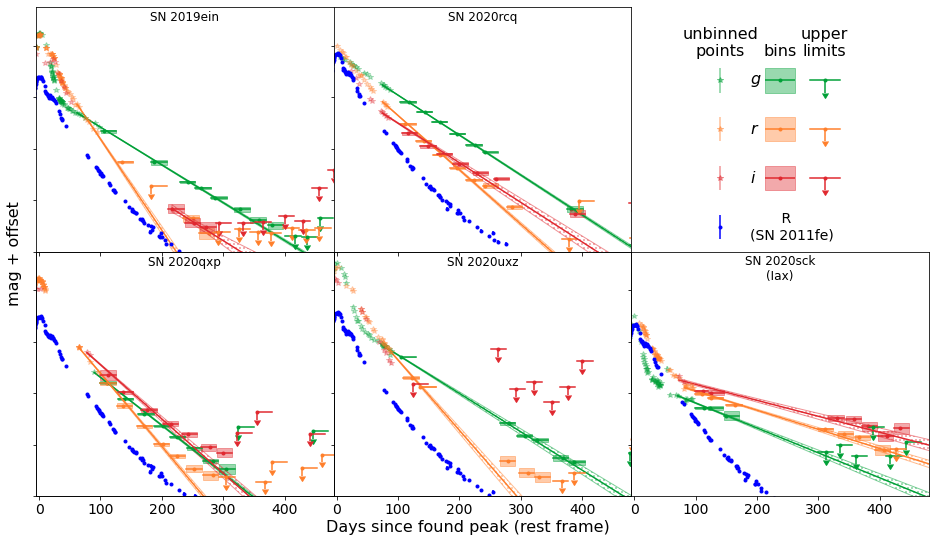
\includegraphics[width=\textwidth]{../Images/chapter_3/kinktails_plots.png}
 \caption{Five objects with kinks in their tails that start to deviate from the assumed decline rate at $\sim$200 -- 250\,d post peak are shown in magnitude space as a function of days since peak. As most of these objects have their peak magnitude blinded, no scaling is shown. A normal radioactive decay model was fitted to these tails, shown as solid straight lines with their $1\sigma$ uncertainty as dashed regions. But as the ejecta opacity changes over time so does the half-life time of the tail, causing a kink seen in the bins which is not reproduced by the model. The arbitrarily normalised \textit{R}-band light curve of SN 2011fe (known not to have CSM interaction from detailed spectral studies) \citep{spec_Lijiang-2.4m} is shown in blue, showing the same shift in decline slope at a similar phase.}
 \label{kink_plots}
\end{figure*}


\subsubsection{Kinked tails}
\label{kink_tails}
This group consists of five objects where the simple tail model, based on the typical decline rate of SNe Ia based on SN 2011fe \citep{Georgios_11fe}, failed to fit the observations at later times. The reason for this failure in four of the events is that there is a slow-down in the $r$- and $i$-band decline rates at $\sim$200 -- 250\,d after peak, which the model does not take into account. The fifth event, SN 2020sck \citep{2020sck_Iax}, is a known SN Iax, a subclass known for having lower ejecta velocities and luminosities, suggesting that the explosion did not necessarily fully disrupt the star \citep{Iax_model_1, Iax_model_2}. This event was flagged because of a slow-down in its decline rate roughly 80 days after the identified peak. The change in slope is visible in all bands and significantly longer than the assumed $t_{1//2} = 50$\,d of normal SNe Ia. The presence of a bound remnant has been suggested to be the cause of similar late-time signatures seen in other SNe Iax \citep{Kawabata_iax14dt, close_Iax, Camacho-Neves_iax14dt}.


The four SNe objects that deviate from the simple tail model are very nearby ($z \leq 0.009$) compared to the majority of ZTF DR2 sample and when using the binned observations they are bright enough to be detected up to (nearly) a year after their first detection. As Rigault et al. (in prep.) are using these nearby events to calibrate their H$_0$ measurement, their peak magnitudes are currently blinded. Figure~\ref{kink_plots} shows the \ztfg-, \ztfr-, and \ztfi-band light curves of these objects in magnitude space. The \textit{R}-band light curve of SN 2011fe \citep{spec_Lijiang-2.4m}, which had a similar change in decline slope, is also shown for comparison. As discussed in \citet{Georgios_11fe}, the radioactive decays produce $\gamma$-rays and positrons, as well as X-rays and electrons that can be thermalised, depositing their energy in the expanding SN ejecta. As the ejecta expand over time they become more transparent, shortening the delay between thermalisation of the deposited energy and the emission of optical radiation. This results in the SN tail slope changing as the opacity changes.

To be able to observe a change in decline slope such as this, a SN has to be both bright and well observed during the time it is visible. The other SNe Ia in our sample at similarly low redshifts have gaps in their observations or the change in slope is not strong enough for the tail fits to fall outside the allowed range of reduced chi-squared values ($\chi^2_\text{red} > 5$) and therefore, are not flagged by the pipeline due to this.


\subsection{Additional tests of promising events}
\label{Additional_tests}
After performing the tests discussed in the previous sections on each event, there are ten objects remaining with an unexplained late-time excess. Light echoes produced by SN light scattering off of nearby dust clouds were considered, but were ruled out as these are typically $\geq$10 mag fainter than the SN at its peak \citep{Patat_light_echoes, 2012cg}. We performed several additional tests on these ten events to try to determine the origin of their late-time excess. The first is using SMP as described in Section \ref{lc_data}. The second is testing for coincidence with an AGN and third is more detailed comparisons with known transient classes. These tests are discussed below and a summary is shown in Table \ref{alt_trans_res}.

\begin{table*}
 \centering
 \caption{Results of the additional tests for the ten promising objects. The host separation is given in $\arcsec$~and converted to kpc using the redshift given in Table~\ref{33_list} and the same cosmology as was used in Sec.~\ref{impact_refdepth}. In the final five columns the similarity of each SN Ia with a late-time excess is compared to different transient classes to see if the late-time signal can be interpreted as another transient. This can be excluded based on an inconsistent colour (1), duration (2), and/or an excessive amount of host extinction (3) needed to obtain the observed magnitudes.}
 \resizebox{\textwidth}{!}{
 \begin{tabular}{lccccccccccccc}
  \hline
   Name & Red. & \multicolumn{2}{c}{Host separation} & \textit{E(B - V)}$_\text{host}$ & AGN $^{(c)}$ & Approx. & SN Ia? & Ib? & Ic? & IIP? & TDE? \\
   & error $^{(a)}$ & ($\arcsec$) & (kpc) & (mag.) $^{(b)}$ & &mag. $^{(d)}$ & \\
   \hline
   SN 2018grt* &no&$0.36\pm0.03$ &$0.32\pm0.02$ & 0.21 -- 0.36 & no &$-$16.5& no (23) & no (23) & no (2) & no (3) & no (13)\\
   SN 2020pkj &no&$0.52\pm0.02$ & $0.28\pm0.01$ & 0.23 -- 0.36 & no &$-$15.4& yes & yes & yes & no (23) & no (13) &\\
   SN 2019ldf* &no&$0.65\pm0.04$ &$0.78\pm0.05$ & $\leq 0.03$ & no &$-$16.4& no (123) & no (123) & no (123) & no (123) & no (13) \\
   SN 2019mse &no&$0.59\pm0.05$ &$1.09\pm0.10$ & 0 & no &$-$17.5& no (2) & no (2) & no (2) & no (2) & yes &\\
   SN 2019rqn &no&$1.39\pm0.08$ &$2.21\pm0.13$ & $\leq 0.04$ & no &$-$16.8& no (13) & yes & yes & no (1) & no (13) \\
   SN 2019vzf &no&$3.89\pm0.08$ &$4.86\pm0.10$ & 0 & yes &-& - & - & - & - & - &\\
   SN 2020awr &yes&$19.60\pm0.04$ &$31.65\pm0.07$ & - &-& - & - & - & - & - & - &\\
   SN 2020alm &no &$0.67\pm0.07$ &$0.85\pm0.09$ & $\leq 0.05$ & no &$-$16.9& no (123) & no (12) & no (23) & no (123) & yes &\\
   SN 2020kzd &yes&$4.67\pm0.04$ &$8.07\pm0.07$ & - &-& - & - & - & - & - & - &\\
   SN 2020tfc* &no &$0.21\pm0.02$ &$0.14\pm0.01$ & $\leq 0.12$ & no &$-$16.8& no (123) & no (12) & no (23) & no (123) & no (3) &\\
   \hline
 \end{tabular}}
 \label{alt_trans_res}
\begin{flushleft}
$^{(a)}$Reduction error: Comparison between the standard light curve reduction and scene modelling identified issues with the baseline correction (see Section \ref{sec:scene_modelling}).\\
$^{(b)}$Estimated assuming the main peak is a normal SN Ia. When correcting for Milky Way extinction and distance is enough to exceed an absolute $g$-band magnitude of $-$19.3, we quote a host \textit{E(B -- V)} = 0 mag. \\
$^{(c)}$The presence of an AGN was estimated using the WISE colours of the host and the criteria of \cite{WISE_crit}.\\
$^{(d)}$Mean absolute magnitude of the \ztfr-band late-time excess after correction for Galactic and host extinction, averaged over the host extinction range considered.\\
\end{flushleft}
\end{table*} 

\begin{figure*}
 \centering
 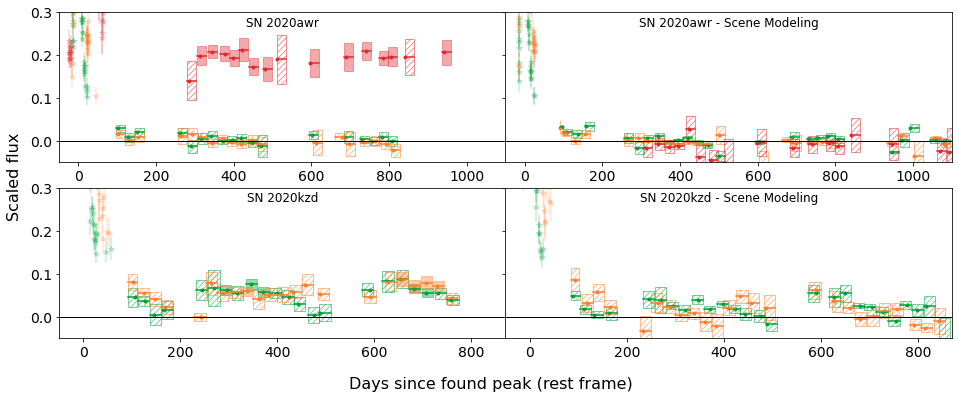
\includegraphics[width=\textwidth]{../Images/chapter_3/other_red_err_plots.png}
 \caption{Two objects whose late-time detections were revealed to be caused by the photometry extraction. The colours are as in Fig.~\ref{kink_plots}. The left side shows the binned forced photometry light curve, and the right side shows the binned SMP light curve. Bins with $5\sigma$ detections are shaded solid, while the non-detections are hashed.}
 \label{other_red_errs}
\end{figure*}


\subsubsection{Scene modelling photometry}
\label{sec:scene_modelling}
To test for issues in data processing, we ran the ten events through the scene modelling pipeline of Lacroix et al.~(in prep.) as discussed in Section \ref{lc_data}. Two SNe Ia (SN 2020awr and SN 2020kzd) were found to have issues with their difference imaging and forced photometry light curves, causing false detections. The detections in both these events are close to the detection limit and therefore, are impacted by even small errors in the baseline placement. The difference imaging (left panel) and scene-modelling (right panel) light curves of these two events are shown in Fig.~\ref{other_red_errs}. 

For SN 2020awr, $\sim$300\,d after the SN peak, the \ztfi-band observations jump up to detections at $\sim$20.3 mag. In contrast to other objects where baseline issues were found, here the offset occurs only for part of the light curve, while the pre-SN baseline has no visible issues. We could not identify a clear reason for this when inspecting the images with \textsc{snap}, and the SN is too far away from the host nucleus for it to be host activity. For the scene-modelling version of the photometry, the jump in the \ztfi-band observations has disappeared completely, showing that there was indeed an unidentified issue with the \ztfi-band data for this object. Since the late-time detections are determined to be spurious, this object is ruled out from having late-time detections.

In the case of SN 2020kzd, late-time detections are present in the \ztfg- and \ztfr-bands for hundreds of days (see Fig.~\ref{other_red_errs}). The SN is in a complex environment with three galaxies close to its sky position, which likely complicates the image subtraction and baseline correction. When SMP is performed on the event the detections disappear and average flux at late times is consistent with zero, showing that the binned forced photometry light curve likely suffered from a wrongly determined baseline correction.

\subsubsection{AGN contamination}
\label{sec:agn_cont}
If a SN explosion site is coincident with a host galaxy that has an AGN, host activity is a likely cause of the late-time detections. Using data from the Wide-field Infrared Survey Explorer (WISE; \citealt{WISE}), \citet{WISE_crit} present a criterion to test if a galaxy hosts an AGN based on the WISE \textit{W1--W2} and \textit{W2--W3} colours, which we apply to our events. One object (SN 2019vzf) is 4.86 kpc of its host centre and its host is a known AGN, with WISE colours of \textit{W1--W2} = $0.55\pm0.03$ and \textit{W2--W3} = $2.90\pm0.04$ mag. In \textsc{snap}, the late-time signal appears to cover both the SN and AGN locations. The AGN contamination is too strong to put any meaningful constraints on the late-time flux at the SN location. We kept the object in our sample until now to test if it is possible to use scene modelling to reduce the AGN contamination. However, this is not possible. We attribute the late-time signal to host activity and disregard it in future discussion. The light curves of SN 2019vzf are shown in Fig. \ref{other_alt}.

\begin{table}
 \centering
 \caption{
 Details of the comparison transients used to test if late-time detections could be explained by another transient at a similar sky position. The first column shows the assumed type of transient, the second shows the transients used to represent each type, the third has the approximate absolute extinction-corrected $r$-band peak magnitudes, and the fourth the reference for each event.}
 \begin{tabular}{lccc}
  \hline
   Type & Name & Peak abs. M$_{r}$ (mag.) & Reference\\
   \hline
   SN Ia & SN 2011fe & $-$18.4 -- $-$19.4 & \citet{spec_HST}\\
   SN Ib & SN 2019yvr & $-$17.9 & \citet{Ib_ex}\\
   SN Ic & SN 2021krf & $-$17.3 & \citet{21krf_ext}\\
   SN IIP & SN 2020jfo & $-$17.8 & \citet{IIp_ext}\\
   SN IIP & SN 2017gmr & $-$18.7 & \citet{2017gmr}\\
   TDE & AT 2018hco & $-$22.1 & \citet{TDE_ext}\\
   TDE & AT 2018zr & $-$20.1 & \citet{TDE_ext}\\
   \hline
 \end{tabular}
 \label{alt_trans}
\end{table} 

\subsubsection{Presence of a sibling close to the SN location}
To test if a previously unidentified sibling transient is causing the late-time detections of the remaining seven objects, we compared their late-time light curves to known classes of transients, including a SN Ia, core-collapse SNe (Type Ib, Type Ic, Type IIP) and two tidal disruption events (TDE). Firstly, we have estimated the amount of potential host extinction from the main SN peak by assuming it was a normal SN Ia with a typical \ztfg-band peak of $-18.8$ to $-19.3$ mag after correcting for the distance to the SN and for Milky Way extinction. These estimated host extinction values are given in Table \ref{alt_trans_res}, assuming R$_\text{V} = 3.1$. The bright end of the absolute peak magnitude gives an upper limit for the host extinction, and the faint end gives a lower limit. After correcting for this range of additional host galaxy extinction, the late-time excesses have mean absolute \ztfr-band magnitudes of $-$15.4 to $-$17.5 mag (see Table \ref{alt_trans_res}). 

After estimating the allowed extinction for each primary SN Ia, we initially assumed that if the late-time excess is due to another transient then it will have the same extinction along the line-of-sight. For these other transients, we used examples of a SN Ia, Ib, Ic, two IIPs, and two TDEs to compare against, with details of the comparison objects described in Table \ref{alt_trans}. The transients chosen to represent their category are all in the typical magnitude range for their type. Two TDEs and SN IIPs were chosen to represent the upper and lower end of the range of peak magnitudes expected for these transients. We use our model for SN 2011fe to represent SNe Ia and test the lower and upper edge of the range of normal SN Ia peak \ztfr-band magnitude.

These comparison objects were chosen as they have well-sampled light curves in the ZTF filters, and literature values for the host extinction. We correct the light curves of the comparison objects using their literature redshifts and their extinction values before correcting for the redshift and extinction of each SN Ia in our sample with a potential late-time excess. We then compare this transient light curve to the found late-time detections to see how well they match. A good match will have a similar magnitude, colour, and duration. 

It could be the case that the suspected sibling was in the same line-of-sight direction, but had a different amount of extinction due to, for instance, exploding behind a cloud that adds additional extinction. We check this by adding enough extinction to match the \ztfr-band detections between the different comparison events and the observed late-time detection and again check if the colour and duration match up, as the observed colour is affected by the extinction. For the TDE comparisons, we allow a host galaxy \textit{E(B -- V)} of up to one magnitude, as was estimated for the ZTF TDE sample of \citet{TDE_host_ext_range}.

For four events (SN 2019mse, SN 2019rqn, SN 2020alm, and SN 2020pkj), the late-time detections are consistent with at least one of the comparison classes, as detailed in Table \ref{alt_trans_res} and shown in Fig.~\ref{other_alt}. We describe them individually in the following sections. The three remaining events (SN 2018grt, SN 2019ldf, and SN 2020tfc) cannot be explained by the presence of a sibling transient and are discussed further in Section \ref{sec:late_time_cand}.


\begin{figure*}
 \centering
 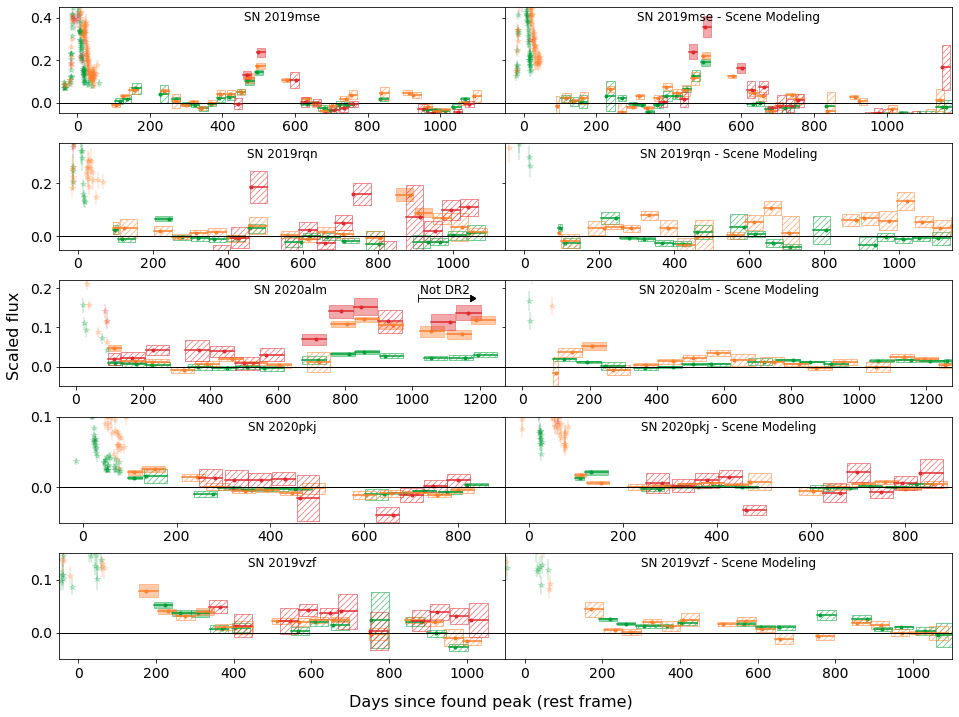
\includegraphics[width=\textwidth]{../Images/chapter_3/other_alt_plots.png}
 \caption{Objects whose late-time detections are explained in the additional tests. The top four rows show the light curves of the objects where a previously undetected sibling transient as an explanation for the late-time observations could not be ruled out, with forced photometry light curves in the left-hand panels and the scene modelling photometry light curves in the right-hand panels. The $5\sigma$ detections are shown as bins with solid uncertainty regions and bins with hashed uncertainty regions are non-detections. The object whose late-time detections are caused by the host galaxy AGN, SN 2019vzf, is shown in the bottom row. The colours are as in Fig.~\ref{kink_plots} with \ztfg band in green, \ztfr band in orange, and \ztfi band in red.}
 \label{other_alt}
\end{figure*}

\subsubsection*{SN 2019mse}
SN 2019mse has late-time detections starting at 450\,d after the peak and lasting $\sim$250\,d in the \ztfg\ztfr\ztfi-bands with an absolute \ztfr-band magnitude of $-$17.5 mag during the excess. Careful re-examination of the difference images show that the late detections are slightly offset (about one pixel) from the SN location, and appear to be on the host nucleus location instead. However, with its WISE colours being \textit{W1 -- W2} = $0.25\pm0.04$ and \textit{W2 -- W3} = $2.44\pm0.09$, the host is determined to not contain an AGN. The scene modelling version of the light curve shows a similar late-time excess, showing that this is not an artefact from the chosen photometric analysis method. 

The late-time signal is detected in all three bands, and its behaviour is very similar in all of them (see Fig.~\ref{other_alt}). Its rise and decline time scales, absolute magnitude, and colours agrees well with the ranges seen for TDE. Together with the observation that the late-time detection are at the host nucleus location, this suggests that a nuclear transient explains the late-time signal adequately.

\subsubsection*{SN 2019rqn}
In the case of SN 2019rqn, there is a short period of detections at 950 -- 1050\,d in the $r$-band after a gap in the observations, declining and fading below the detection significance within 100\,d of the first detection. Nothing is detected at a $\geq 5 \sigma$ level in the \ztfg- or \ztfi-band observations. The \ztfi-band SMP light curve had its host contribution not completely subtracted, causing a flux offset in the data points. We therefore do not consider the SMP \ztfi-band further. The data points in the \ztfg- and \ztfr-band light curve have slightly larger uncertainties in the SMP version, causing the main SN light curve to fall below the 5$\sigma$ threshold at an earlier epoch resulting in fewer individual points visible (Fig.~\ref{other_alt}). Similarly, larger uncertainties for the SMP prevents the detection of a late-time \ztfr-band signal.

Assuming a sibling exploded during the gap in the observations between 870 and 950\,d post peak, SNe Ib and Ic with \textit{E(B -- V)} $\leq 0.3$ mag extinction in the \ztfr-band can fit their tail to match the observed detections in the \ztfr-band without being excluded by the \ztfg-band and \ztfi-band non-detections. Therefore, we cannot rule out a sibling as the source of the detected late-time signal.

\subsubsection*{SN 2020alm}
The late-time signal in SN 2020alm is seen in all three bands, beginning at $\sim$750\,d after the peak and lasting for at least 300 d. There is a gap of 80\,d in the observations immediately before the period of activity. The detections slowly rise to a plateau. Our initial analysis only included data for SN 2020alm up to $\sim$1000\,d after the peak. However, when this object was identified as having late-time detections, the light curve pipeline was rerun and it was found to be still bright at later times, with significant detections in the \ztfr- and \ztfi-bands, but not above 5$\sigma$ detections in the \ztfg-band. The \ztfi-band SMP light curve contained a significant flux offset, as the host was not fully subtracted. We therefore do not further consider this band. The binned SMP \ztfr-band light curve fails to reproduce the late-time detections found in the forced photometry light curve. However, the \ztfg-band detections are recovered in the SMP. The SN is close to the host nucleus at 0.66$\arcsec$~(0.85 kpc) offset at the redshift of the SN, but the WISE colours of \textit{W1--W2} = $0.06\pm0.04$ and \textit{W2--W3} = $2.42\pm0.12$ place it far outside the AGN region. 

As SN 2020alm was still active while our analysis was on-going, we obtained two spectra using the Optical System for Imaging and low-Intermediate-Resolution Integrated Spectroscopy (OSIRIS) instrument on the Gran Telescopio CANARIAS (GTC) at Roque de los Muchachos in La Palma on 26 July 2023 using the R1000R grism. As the spectrum is heavily dominated by the host galaxy, we subtracted a rebinned spectrum of the host taken by the Sloan Digital Sky Survey (SDSS, \citealt{SDSS-I-II, SDSS_DR4, SDSS_telescope, SDSS_Spectograph}) in 2003, well before the SN occurred. We confirmed successful host subtraction by checking for residual \NaID~and \MgI~${\lambda5175}$ absorption lines and found that no residual features were present. A more detailed explanation is given in Appendix \ref{spec_sec}.

The resulting spectrum shows an excess that is stronger towards longer wavelengths (Fig.~\ref{ZTF20aaifyfx_spec}). This is consistent with the broadband photometry finding an brighter excess in the redder bands, while the \ztfg-band remains within the noise after binning the observations. There is some excess in the narrow [\NII]~${\lambda\lambda6548,6583}$, \Halpha~and [\SII]~$ {\lambda\lambda6716, 6730}$ emission lines, but we lack the resolution to check if this is significant. There is no visible additional \Halpha~component in the spectrum, which would be indicative of CSM interaction. Integrating the spectrum over the \ztfr- and \ztfi-band efficiencies gives an \ztfr -- \ztfi colour of 0.6 mag, which is within $3\sigma$ of the value found in the latest photometry bin.

\citet{TDE_host_ext_range} show that TDEs generally have a \ztfg -- \ztfr colour of zero and can have featureless spectra. We approximate a TDE by a flat line in order to estimate the amount of extinction needed to generate a red excess similar to the spectrum. We find that the general shape of the spectrum can be approximated with $0.6 < \text{E(B -- V)}_\text{host} < 1$ mag. This would mean an absolute \ztfr-band magnitude of $-18.8 > M_r > -19.8$ mag. \citet{TDE_host_ext_range} show that both this amount of host extinction and late-time brightness are possible for TDEs. They also show that it is possible for a TDE to rise and fall back down within the 80\,d gap in observations, although this is seen in fainter TDEs than corresponding to our estimated absolute magnitude range.

The TDE sample of \citet{TDE_host_ext_range} did not contain a single object that matches our late-time detections in duration and luminosity in SN 2020alm. However, it is possible to combine parts of different TDEs together to make a TDE that peaked and decayed within the 80\,d gap and levelled out by the time it became observable again. Based on this, a TDE is a plausible explanation for the late-time signal detected in this object.


\subsubsection*{SN 2020pkj}
In the case of SN 20120pkj, the first \ztfr-band bin with a detection is the end of the normally declining tail, but after the first bin the detections rise slightly in the next \ztfr-band bin (Fig.~\ref{other_alt}). None of the binned photometry for the \ztfg- and \ztfi-bands give significant detections. Unfortunately, there is a gap in the observations immediately after the \ztfr-band detections preventing us from following its evolution closely at these phases. When it became observable again at $>$200 d, no significant detections were found in any band. The duration of the transient is at least 75\,d and could be up to 150 d. In the SMP light curve of this object, a similar rise at the same epochs is recovered, though it is found in the \ztfg-band instead of the \ztfr-band. This is likely due to the low significance of these detections at just 5.8-$\sigma$ in the \ztfr-band in the forced photometry and 5.2-$\sigma$ in the \ztfg-band in the SMP, showing that they are just on the detection limit of our binning technique.

With a redshift of $z = 0.02456$, this object is nearby enough for the end of the tail to be visible in the bins at 100 days. This could explain why the first bin is a detection, but the slight increase is still unexpected for a normal SN Ia decline tail. While the second bin is marginally consistent with our tail fit, a slight but steady increase can be seen in the unbinned flux values as well, suggesting that the brightening is real.

Assuming that the detected part of the late-time signal is the brightest part of a sibling transient, the tested transients need significantly more extinction of $\sim$ 3 to 6 mag in the \ztfr-band (depending on the comparison transient) than was found for the main SN Ia peak. However, the $\sim 80$\,d gap is long enough for a Type I sibling SN to peak higher during the gap and dim again before observations resumed. The other transient could have just started when it stopped being observable, and declined below the detection limit when the location became observable again. Since there is no constraint on the magnitude, this could work with any amount of extinction. Therefore, we cannot rule out conclusively that the late-time detections are due to another transient.


\subsubsection{Late-time interaction candidates}
\label{sec:late_time_cand}
Finally, we present the three objects (SN 2018grt, SN 2019ldf, and SN 2020tfc) whose late-time detections could not be explained by any of the explanations discussed above. Their light curves are shown in Fig.~\ref{candidates}, and the colours of the late-time detections in Fig.~\ref{candidate_colours} and the SMP light curves for SNe 2019ldf and 2020tfc in~\ref{final_candid_SMP}. A scene modelling analysis could not be performed for SN 2018grt due to it exploding early in the ZTF survey. The forced photometry pipeline uses images obtained during the ZTF commissioning phase as templates but the SMP does not. We present these three objects as late-time interaction candidates as there are no spectra of these objects at these late times to confirm the presence of features consistent with CSM interaction.

By using the estimated mean absolute $r$-band magnitude after removing all extinction effects (see Table \ref{alt_trans_res}) we can estimate the required \Halpha~flux assuming that it is the source of all the detected flux in the $r$-band, and that the emission line has the same width as was used during the simulations. The identified strength of the signal is compared to the \Halpha~signal detected in SN 2015cp for each of the events.

\begin{figure*}
 \centering
 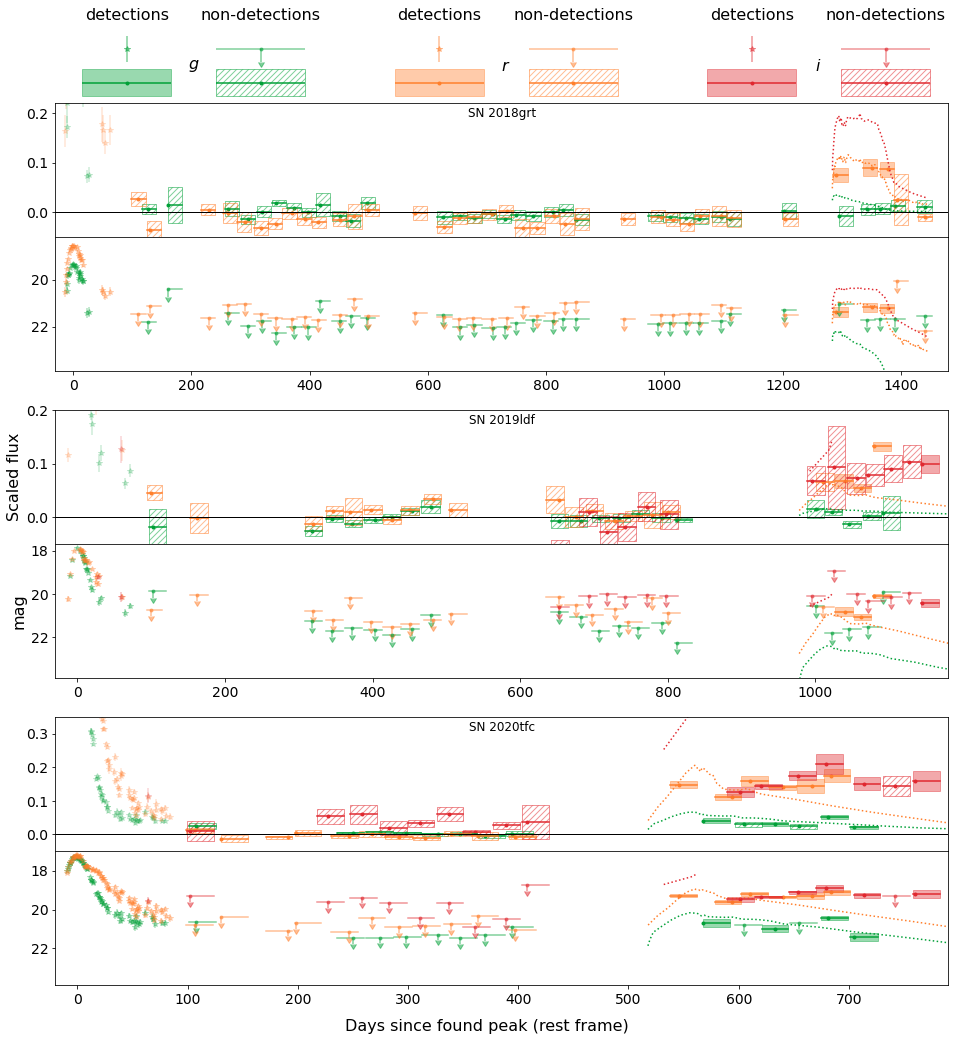
\includegraphics[width=\textwidth]{../Images/chapter_3/candid_plots.png}
 \caption{Three candidate objects, shown in magnitude and flux space. All three have significant detections ($\geq5\sigma$) after a period of observations consistent with zero flux. From the alternative explanations the best fitting alternate transients are shown in dotted lines. For SN 2018grt this is the Type IIP SN 2017gmr, for SN 2019ldf and SN 2020tfc this is the TDE AT 2018hco.}
 \label{candidates}
\end{figure*}

\begin{figure*}
 \centering
 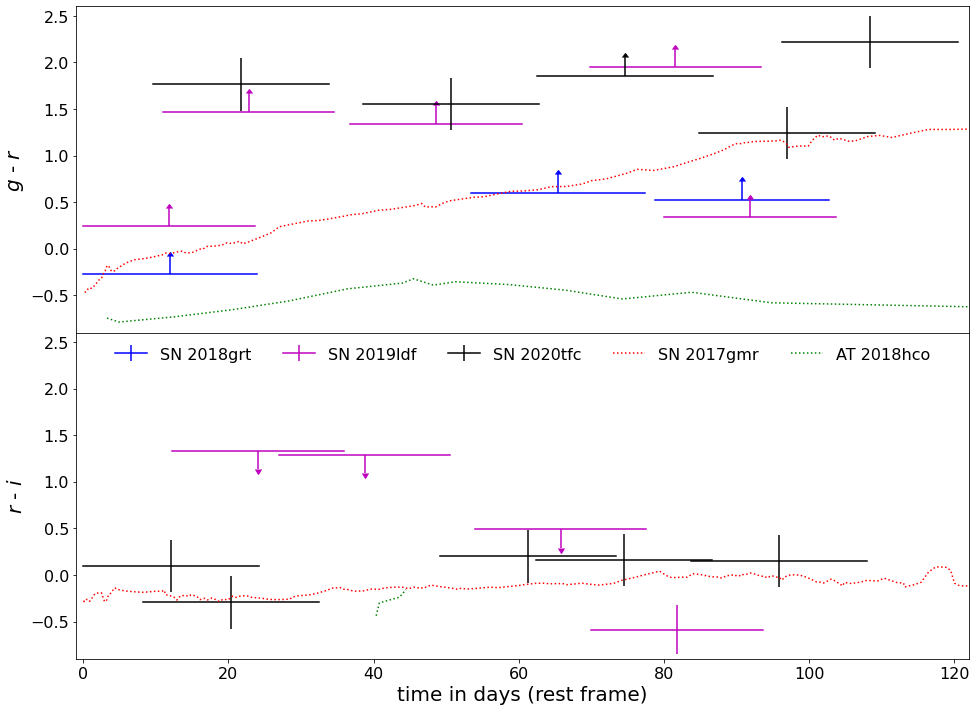
\includegraphics[width=13cm]{../Images/chapter_3/candid_colours.png}
 \caption{Colour curves of the three candidate objects, together with the colours of the best fitting alternate transients. The top and bottom panels show $g$-$r$ and $r$-$i$, respectively. The first bin for each object starts at zero days, but the bins can be shifted horizontally in an attempt to better fit the colour curve of the transient compared against (given that this is allowed by the rest of the light curve). Bins whose mean observation dates are closest to each other are used to calculate the colour, provided that these bins overlap in time. If there is a detection in only one band used to calculate the colour while the other is a non-detection, the result is a lower or upper limit.}
 \label{candidate_colours}
\end{figure*}

\subsubsection*{SN 2018grt}
The late-time signal of SN 2018grt is only detected in the \ztfr-band, the \ztfg-band stays around zero flux, and there are no \ztfi-band observations at these phases. The first detection in the \ztfr-band begins at 1350\,d post peak with a magnitude of $21.4\pm0.2$ (absolute magnitude of $-$16.4 mag). It varies little over the $\sim 100$\,d period where it is detected, after which it returns to zero flux within 50\,d. The SN is close to the host nucleus with an offset of 0.35$\arcsec$~(0.32 kpc) but its host colours place it well outside the expected AGN region. Checking the difference images with \textsc{snap} shows that the host nucleus and SN location differ by $\sim$1 pixel. 

The late-time detections are $\sim 2.5$ mag below the main SN peak. If the late-time signal is due to another SN Ia or a TDE, it would require a significantly higher extinction value than was found for SN 2018grt itself. In addition, this object shows a sudden drop in the \ztfr-band, which is not normal behaviour for a TDE. Most of the other transient types cannot reproduce the plateau followed by the sharp decline only detectable in the \ztfr-band, apart from a SN IIP, where the plateau of SN 2017gmr has nearly the same time span. However, to fit the observed magnitude with a IIP SN, it would require a host $ E(B$ -- $V)$ that is three times higher than what was found for SN 2018grt, making this scenario less likely to be the case. Therefore, we conclude that late-time CSM interaction is a plausible scenario for the late-time signal in this object.

If we assume $0.21 \leq E(B$ -- $V)_\text{host} \leq 0.36$ mag and that the \ztfr-band signal is produced only by an \Halpha~emission line with a similar width to the one used in our simulations in Section \ref{simulation}, we estimate the strength of the emission to be much stronger than SN 2015cp, at 60 to 100 times its emission strength. However, there are examples of SNe Ia-CSM with interaction strengths this strong, for example, SN 2020eum was within this range \citep{Ia-CSM_BTS}.


\subsubsection*{SN 2019ldf}
SN 2019ldf has late-time detections in the \ztfr-band beginning at 1050\,d after the peak and lasting for about 100 d, with an additional increase in brightness towards the end. There is a single $5\sigma$ detection in the \ztfi-band but there are a number of lower significance detections coeval with the \ztfr-band detections. These detections are directly after a long period without observations due to the object being behind the Sun. Nothing is detected in the \ztfg-band during the time of the rise in the \ztfr band. The binned SMP light curve recovers these late-time \ztfr-band detections, and a single \ztfi-band detection, showing that these detections are not specific to the photometry method.

We compared the properties of the late-time detections to those of our comparison transient objects. Even if we assume that a SN exploded during the gap in observations in order to avoid needing a significantly larger \textit{E(B -- V)}$_\text{host}$ value, SNe evolve too much over a period of 100 days to explain the detections. In addition, detections would also be expected in the \ztfg-band, which have not been found. 

A TDE could fit the detections if it was intrinsically bright but heavily extincted, as this could explain the red colour and absence of signal in the $g$-band. However, SN 2019ldf is offset from the host nucleus by 0.65 $\arcsec$~(0.78 kpc) and inspection of the difference images using \textsc{snap} shows that the late-time signal is more consistent with the SN location than the host nucleus location, disfavouring the TDE explanation. Therefore, we conclude that the late-time signal could be due to late-time CSM interaction.

The late-time detections persist until the end of the observation window. To determine if there were still signs of interaction once it was visible again, we obtained \ztfg- and \ztfr-band photometry with the EFOSC2 imaging spectrograph \citep{EFOSC2} on the ESO New Technology Telescope (NTT) in La Silla, Chile on 2023 May 19 as part of the extended Public ESO Spectroscopic Survey of Transient Objects+ (ePESSTO+; \citealt{PESSTO}).

To examine whether the SN is still detected in our images from May 2023, we used image subtraction techniques. Due to the lack of reference images in the \ztfg- and \ztfr-band filters from EFOSC2, we used images from the DESI Legacy Imaging Surveys Data Release 9 \citep{DESI-Legacy_Imaging_Surveys}. After aligning the images, we subtracted them from each other with the High Order Transform of Psf ANd Template Subtraction code version 5.11 \citep[\textsc{hotpants};][]{HOTPANTS}. We measured the brightness in the difference images using aperture photometry. The photometry was calibrated against stars from DESI Legacy Imaging Surveys. The EFOSC2 and DESI Legacy Imaging Surveys filters are not identical which might add an unknown systematic to the reported photometry. The $5\sigma$ upper limits are $m_g = 24.7$ and $m_r = 24.3$ mag at 1397 days after the peak, with no detection in either band. This means that the signal has disappeared at this time, and thus could have lasted, at most, for about 500 days.

Assuming that the \ztfr-band signal is entirely due to the \Halpha~emission, we estimate it to be $\sim$60 times as strong as the late-time interaction found in SN 2015cp. However, this assumption is very simplistic, as it completely disregards the rise in the \ztfi-band and therefore it is only a first order estimate.


\subsubsection*{SN 2020tfc}
This object has late-time \ztfg\ztfr\ztfi-band detections, beginning at 550\,d after the peak and lasting for at least 250 days. While the \ztfr- and \ztfi-bands are at more or less the same magnitude, the \ztfg-band detections are about 1.3 mag fainter. This immediately poses an issue for any alternate transient considered, as either there is a low amount of extinction and a weak \ztfg-band signal, or there is a high amount of extinction and the intrinsic signal is even brighter in the \ztfi-band. This, combined with the fact that the signal lasts for several hundreds of days with little variation, disfavours a SN as an alternate transient explanation. The intrinsic colour also heavily disfavours a TDE as these objects tend to have a similar intrinsic brightness in the \ztfg-, \ztfr-, and \ztfi-bands. In the binned SMP light curve the late-time detections were confirmed in the \ztfg-band. The SMP \ztfi-band data points have a large scatter, most likely due to uncertain background removal because of a low number of available images for the SMP template. Therefore, we do not consider them further in our analysis. In the \ztfr-band SMP light curve, the data points are below our 5$\sigma$ cut-off for detections, although one is very close to our limit at 4.6$\sigma$. However, the \ztfg-band detections seen in the forced photometry are confirmed by SMP suggesting a real signal is present at late-times in at least this band, and at lower significance in the \ztfr band. 

Similar to SN 2020alm, the late-time signal was on-going during our analysis but unfortunately there is no archival host galaxy spectrum available to compare to. As the host dominates the late-time signal (the SN is at a distance of 0.28$\arcsec$ (0.21 kpc) from the host nucleus) and cannot be removed using difference imaging or SMP as for the photometry, this prevented us from taking a spectrum of the late-time signal. With all alternate explanations ruled out or severely challenged by observations, the late-time CSM interaction remains as a plausible explanation for these late-time detections. 

If we assume that the \ztfr-band signal is due to \Halpha~emission only, the interaction is estimated to be 110 to 150 times as strong as the interaction found in SN 2015cp. This is by far the strongest of the three, but again this simple assumption is unrealistic as it completely ignores the measured \ztfg- and \ztfi-band signal that suggests a contribution from a continuum or other spectral lines to the late-time signal. 
 
\begin{table*}
 \centering
 \caption{Parameters used for rate estimation simulations for each object.}
 \resizebox{\textwidth}{!}{%Scale table to page width
 \begin{tabular}{lcccccc}
  \hline
  Object & Start epoch & Duration & Strength & $N_\text{sample}$ & late-time CSM & late-time CSM\\
   & (d) & (d) & (SN 2015cp) & & fraction & rate (Gpc$^{-3}$ yr$^{-1}$)\\
  \hline
  SN 2018grt (worst) & 1\,375$^{*}$ & 100 & 60 & 748 & $0.0084_{-0.0041}^{+0.0183}$ & $203_{-97}^{+438}$\\[4pt]
  SN 2018grt (best) & 1\,275$^*$ & 200 & 100 & 988 & $0.0015_{-0.0007}^{+0.0032}$ & $36_{-18}^{+76}$\\[4pt]
  SN 2019ldf (worst) & 1\,050$^*$ & 200 & 60 & 1\,931 & $0.0019_{-0.0009}^{+0.0036}$ & $45_{-22}^{+87}$\\[4pt]
  SN 2019ldf (best) & 875$^*$ & 500 & 60 & 2\,505 & $0.0023_{-0.0011}^{+0.0038}$ & $54_{-26}^{+91}$\\[4pt]
  SN 2020tfc (worst) & 550 & 250 & 100 & 3\,439 & $0.0004_{-0.0002}^{+0.0009}$ & $10_{-5}^{+22}$\\[4pt]
  SN 2020tfc (best) & 450 & 500 & 150 & 3\,493 & $0.0003_{-0.0002}^{+0.0008}$ & $8_{-4}^{+20}$\\
  \hline
 \end{tabular}
 }
\begin{flushleft}
For each of the three SNe we assumed a worst and best case scenario for detecting them in our sample, giving upper and lower limits for a simulated observing campaign. The efficiency curves generated from these simulations were then used to determine the intrinsic fraction of SNe Ia with late-time CSM interaction in an MCMC process, with the assumption that only one object was recovered in a sample size that is the same as the amount of DR2 objects with observations after the start epoch ($N_\text{sample}$). The last two columns show the found late-time CSM interaction fraction of the total SN Ia rate and the late-time CSM interaction rate.\\
$^*$When the start epoch of the late-time excess is $>$750 d, 750\,d is used as the start epoch because of limitations of the available ZTF survey plan. See Section \ref{rates_csm} for more details.\\
\end{flushleft} 
 \label{rate_sims}
\end{table*}

\subsection{Late-time CSM interaction rates based on our candidate objects}
\label{rates_csm}

 We identified three objects (SNe 2018grt, 2019ldf, and 2020tfc) with potential late-time CSM interaction signatures. For SN 2018grt and SN 2019ldf, these detections were in the \ztfr-band (with no \ztfi-band data available for SN 2018grt and low significance \ztfi-band detections for SN 2019dlf). For SN 2020tfc, late-time detections were found in all three bands (\ztfg\ztfr\ztfi). In our initial simulations to determine our recovery efficiency (Section \ref{simulation}), we made the assumption that any CSM interaction would be dominated by \Halpha~emission that would be present in only the \ztfr-band up to $z \sim$ 0.07 and in the \ztfi-band beyond that. This was based on the dominant interaction signatures seen in SNe Ia-CSM and also the one event with late onset interaction, SN 2015cp \citep{2015cp}. 

In \citet{2015cp}, the \CaII\ NIR triplet emission was also identified in its spectra, along with emission consistent with \MgI~$\lambda5175$. \cite{2018ApJ...868...21H} speculated that although the \CaII\ NIR region was very noisy, the \CaII\ emission may be a similar strength to the \Halpha~emission. For SN 2019ldf at a redshift of 0.057, the \CaII\ NIR triplet, if present, would be partially shifted out of the \ztfi-band, which could potentially explain its low-significance \ztfi-band detections. SN 2020tfc is at lower redshift (0.031) so the \CaII\ NIR triplet would fall completely in the \ztfi-band and could potentially be the source of the \ztfi-band detections. The strength of the potential \MgI~$\lambda5175$ line in SN 2015cp was weak and not well constrained \citep{2015cp} but could potentially result in a weak signature in the \ztfg-band. However, without spectral confirmation this is only speculation.

The other difference between our initial simulations for determining recovery efficiency and the observed detections in our three candidate late-time CSM objects is that the late-time CSM interaction signature is much stronger in our observed events. In our three candidates, the late-time signal is between 2 to 3 magnitudes below the SN peak magnitude, while in the simulations with strongest interaction the signal was about 4.4 magnitudes below the peak.

It is clear from our candidate events, that there is significant diversity (detected bands, timescales and strengths) in their potential CSM signatures and without knowledge of their underlying spectra (e.g. emission lines that are present), it is difficult to develop spectral models and run simulations covering this full diversity. Therefore, although very simplistic and ignoring other potential emission lines occurring in the \ztfg- and \ztfi-bands as were seen in SN 2015cp \citep{2015cp}, we focussed on \Halpha~emission dominated models and the corresponding \ztfr-band detection efficiency to estimate a rate of late-time \Halpha~emission dominated CSM interaction based on our three candidate objects. We use the same underlying spectral model (SN 2011fe combined with \Halpha~emission) as detailed Section \ref{simulation} in further \textsc{simsurvey} simulations but constrain the strength and timescale of the CSM signature based on our three events. In Table \ref{rate_sims}, we show the range of start epoch, duration and strength (dependent on assumed host galaxy extinction) simulated for each event. For each of the three objects, we take the worst case scenario (shortest, weakest, latest start epoch) and the best case scenario (longest, strongest, earliest start epoch) allowed by the constraints from the data to estimate a worst and best case scenario recovery efficiency for each object.


\begin{figure*}
 \centering
 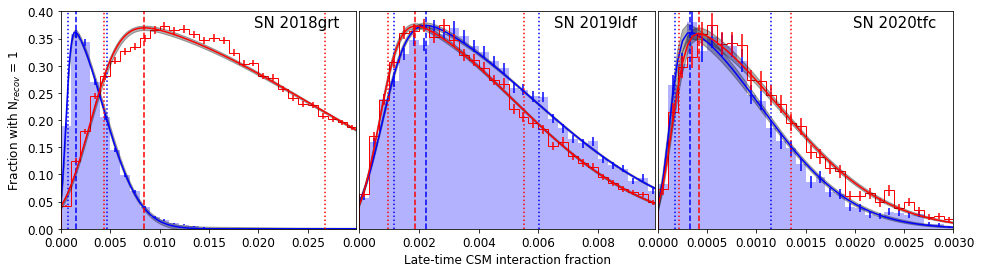
\includegraphics[width=\textwidth]{../Images/chapter_3/rateplots.png}
 \caption{Fraction of MCMC realisations per bin that resulted in one object being recovered in a sample with the same size as the effective DR2 sample size as a function of the late-time CSM interaction fraction. The best and worst case scenario for each object is shown in blue and red, respectively. A skewed normal distribution fit with a $1 \sigma$ uncertainty band is shown for each scenario, and the dashed and dotted lines give maximum and 68 per cent confidence interval of these distributions, respectively. The distributions continue on the right side of each plot.}
 \label{rate_fig}
\end{figure*}

Since the available ZTF survey plan for our simulations only spans 1004 d, we cannot set the interaction signal to start at phases after this as the interaction would never be observed. Therefore, we choose to start the interaction in our simulations no more than 750\,d after the peak. This is done to ensure there is a decent chance to observe an event until after the interaction has started, while still being able to apply a good baseline correction. As the interaction is by far the dominant source of light at these epochs, changing the start date of the interaction in this way has little effect on the total brightness of the SN. However, it does affect the number of objects observed by allowing more objects to have observations at later times, when the interaction occurs. This is a redshift independent effect, but will impact the resulting recovery fraction function. To account for this, we only consider objects with observations after the start of the interaction, and remove those where the simulation limits prevent any possible late-time detection. While changing the interaction start date has increased the number of objects that satisfy this condition, there are still some objects that do not due to e.g. being in a sparsely observed field.

Not all objects in the DR2 have detections up to the time after the peak where the interaction was detected in the three final candidates. Similar to the simulation, in order to get a proper estimate of the rate we can only consider the objects that could have been found interacting ($N_\text{sample}$), and remove those without observations this late after the peak. This gives us an effective sample size that is smaller than the full DR2, and is listed in Table \ref{rate_sims}.

The expected number of observed objects with late-time interaction in a sample $N_\text{recov}(N_\text{sample}, \eta(z))$ is a function of the efficiency and the intrinsic rate, which in turn is a fraction of the total SN Ia rate. If we assume the SN Ia rate from \citet{SNIa_rate} as in our initial simulations and that the fraction of these showing late-time interaction, $f$, is redshift independent, then the only $z$ dependency is in the efficiency of our pipeline. In a similar approach to \citet{SLSN_rate} and \citet{Ca-rich_rate}, we run a Markov chain Monte Carlo (MCMC) simulation with $10^7$ realisations for each scenario to find the fraction of interacting SNe that best explains our findings.

In each realisation of the MCMC, we draw $N_\text{sample}$ objects, and assign a redshift to each object according to the distribution from \citet{SNIa_rate}. For each object we also draw two random numbers from a flat distribution between zero and one. The first random number is used to decide if the object was interacting, and the second to decide if any interaction would have been recovered. Interaction is true if the random number is below the chosen value for $f$ for that realisation. Recovery is true if the second random number is below $\eta(z)$ at the $z$ of the object (e.g. if the recovery efficiency is 0.7 at the SN redshift, a drawn number below 0.7 will result in a detection if the object was interacting). The number of recovered objects with interaction can be found by counting the objects for which both interaction and recovery is true, while the actual number of interacting objects can be found by counting the objects where interaction is true.

Figure \ref{rate_fig} shows per bin the fraction of realisations that resulted in one object being recovered as a function of late-time CSM interaction fraction with the best and worst scenario parameters for the three discovered events. We approximate them by fitting a skewed normal distribution and use the fit to estimate the peak of the distribution and the 68 per cent confidence interval on either side. These values are quoted as a fraction of the total SN Ia rate and as the late-time CSM interaction rate in the last two columns of Table \ref{rate_sims}.


\section{Discussion}
\label{discussion}

In this section, we first discuss the overall rate of CSM interaction signatures found in our analysis (Section \ref{discuss_interaction}) and some of the properties of the three SNe Ia displaying these unexplained late-time detections (Section \ref{discuss_prop}). 

\subsection{Late-time interaction is rare in SNe Ia}
\label{discuss_interaction}

In our study of the $\sim$3500 SNe Ia in the ZTF DR2 with photometry at $>$100 d, we identified three objects (SN 2018grt, SN 2019ldf, and SN 2020tfc) for which late-time CSM interaction is the best explanation for their detected late-time flux excesses. However, as each of these has significantly different parameters for the interaction, they have to be treated separately when trying to estimate the rate of late-time CSM interaction in SNe Ia (Section \ref{rates_csm}). Except for the worst case scenario of SN 2018grt, the identified rate for all cases agree with one another within the uncertainty, with the fraction of SNe Ia showing late-time \Halpha-dominated CSM interaction between $0.03^{+0.08}_{-0.02}$ and $0.23^{+0.38}_{-0.11}$ per cent. This is similar to what was found by \citet{Ia-CSM_BTS} in their Ia-CSM sample, and agrees with the upper limit set by \citet{2015cp} with their discovery of the late-time interaction in SN 2015cp. Some objects were disregarded as we could not definitively determine that they were not due to a sibling transient. Therefore, there could be a handful of additional objects displaying strong late-time \Halpha-dominated CSM interaction that were not included in our rate estimates but this would double the rate at most. Therefore, we estimate that the intrinsic rate of late-time \Halpha-dominated CSM interaction in SNe Ia is $<0.5$ per cent.

The identified late-time signals that are consistent with CSM interaction occurred between 1.5 to over 3.5 years after the original SN peaked. If we assume that the SN ejecta have a velocity of the order of $10^4$ km s$^{-1}$, the distance at which the CSM shell resides is of the order of $10^{17}$ cm. As CSM moves slowly, this means it must have been ejected from the system a long time ago. The further out the shell is from the progenitor system, the more mass is contained in even a thin shell. This is especially true when one considers that in order to get a detectable signal from the interaction, the CSM density cannot be too low. At these distances, light travel time effects also become significant, and a short interaction with a thin shell will be smeared out over a long time. Unfortunately, since we have only partial constraints on the interaction timescales and CSM mass estimation from an interaction signature is far from straightforward, we do not attempt to provide a CSM mass estimate.  

An interesting aspect of the late-time detections in our three candidates is their inferred strength. While our model is likely an oversimplification by trying to explain the entire \ztfr-band signal using only a narrow \Halpha~line, it is clear that the signal is much stronger compared to the one found in SN 2015cp, especially when there are other band(s) at a similar magnitude. Interaction this strong is not unprecedented though, SN 2020aekp for instance, starts to plateau around 50 days after peak at an absolute magnitude M$\sim-18.5$ in all three ZTF bands \citep{Ia-CSM_BTS} and holds this plateau for several hundreds of days. Most of the known SNe Ia-CSM presented in \citet{Ia-CSM_BTS} have detections in multiple bands, and the spectra presented show more than just an \Halpha~line coming from the CSM interaction. CSM around a SN Ia also does not have to be spherically symmetric, especially in a scenario where material has been stripped and partially lost from the donor star in the progenitor system. \citet{IIn_asym_CSM} show for SNe IIn that if the CSM mostly resides in a disk, only the ejecta travelling in the direction of the disk will be slowed down and interact while ejecta at higher inclinations continues to expand normally. 

The colour curves for the late-time detections in our three objects (Fig.~\ref{candidate_colours}), show that $g - r \sim$1.7 mag for SN 2020tfc, with limits of $g - r > 0.5$ and 1.5 mag for SN 2018grt and SN 19ldf, respectively.
For the two objects with $i$-band observations, $r-i<0.5$ mag. The SN Ia-CSM sample of \cite{Ia-CSM_BTS} had late-time ($>$300 d) $g - r$ colours of $0 - 0.5$ mag, which are similar to SN 2018grt but bluer than SN 2019ldf and SN 2020tfc. \citet{Kool_He_CSM} find $g-r\sim-1$ mag and $r-i\sim0.5$ mag at late times for the He-interacting Ia-CSM SN 2020eyj. When taking into account the host galaxy extinction that they identify, it becomes even bluer and is much bluer than our three objects.


\subsection{Properties of SNe Ia with late-time interaction}
\label{discuss_prop}

The three SNe Ia with late-time flux excesses that cannot be explained by other scenarios have SALT2 light curve fitter $x_1$ and $c$ values that are generally typical of normal SNe Ia (Rigualt et al.~in prep.). However, the $c$ value of SN 2018grt of 0.61 $\pm$ 0.03 is at the high end and would be excluded from cosmological analyses. We also identified significantly more host extinction for this object than for the other two based on their luminosities at the peak. 

All three candidates are found at small projected distances from their host nuclei. While the small sample size might be used to explain part of this observation, the mean projected distance of all objects in the ZTF DR2 is 6.3 kpc (Rigault et al.~in prep.). The chance for our three objects to be at most 0.8 kpc from the host is $<1$ per cent, suggesting that objects with late-time interaction have a preference for small host separations, the detections are caused by nuclear variability, or they are caused by bad host subtraction. The location of the late-time signal is too close to the host nucleus to distinguish which location the late-time signal is more consistent with by using \textsc{snap}. The host galaxy colours are inconsistent with being AGN and the properties of the late-time detections cannot be easily explained by known nuclear transient classes such as TDEs. It is possible that by going to deeper limiting magnitudes with our light curve binning that we have identified previously unstudied nuclear variability but this cannot be confirmed. Imperfect template subtraction can occur to galaxy centres, resulting in a dipole artefact. However, these are easily recognisable with \textsc{snap}, and this possibility was ruled out for our three candidates. Therefore, we conclude that that a likely interpretation is that there may be something intrinsic to SNe Ia exploding in these environments that produces late-time CSM interaction but further samples are required to confirm. 

The morphologies of the host galaxies of the candidate events are broadly elliptical or spheroidal in nature with no signs of spiral arms. The galaxies have stellar masses of 4 $\times$ 10$^9$, 6 $\times$ 10$^10$, and 2 $\times$ 10$^{10}$ M$_\odot$ for SN 2018grt, SN 2019ldf, and SN 2020tfc, respectively. These host masses are all within the bulk of the masses of the ZTF DR2 SN Ia sample (Rigault et al.~in prep.). The hosts of the known H-rich Ia-CSM sample have stellar masses of $\sim$3 $\times$10$^8$ to 3 $\times$ 10$^{10}$ M$_\odot$, consistent with our objects \citep{Ia-CSM_BTS}. SN 2020eyj, the He-interacting and radio detected SN Ia-CSM \citep{Kool_He_CSM} also had a very small offset from its host of $0.57\pm0.02\arcsec$ ($0.36\pm0.01$ kpc). Its host only has a WISE \textit{W3} upper limit so it cannot be excluded from having an AGN present. It is a compact star forming galaxy with a mass of $\sim$6 $\times$ 10$^7$ M$_\odot$, which is lower than the typical Ia-CSM range \citep{Ia-CSM_BTS}. 

The hosts of the three candidate events all have WISE \textit{W1 -- W2} $\approx0$ mag. SN 2020tfc has \textit{W2 -- W3} of $\sim$0.8 mag, while the other two have only limits with \textit{W2 -- W3} $>$ 1.2 mag. Based on Fig.~2 of \cite{Irani_wise}, this places them in the overlap region between elliptical and spiral host properties from the galaxy sample of \cite{Lintott_galaxyzoo}. The vast majority of Ia-CSM sample of \cite{Ia-CSM_BTS} has \textit{W2 -- W3} colours of $>$ 1 mag, again broadly consistent with our sample. However, the morphologies of our candidate events do not show evidence for spiral arms and their overlap between ellipticals and spirals in the \textit{W2 -- W3} parameter space suggest they may come from different, older stellar populations than the known Ia-CSM events \citep{Kool_He_CSM, Ia-CSM_BTS}. However, to prove that these are different populations requires a larger sample. 

\subsection{Limitations of the analysis}
Since there is no good model of a Type Ia SN interacting with CSM at late times that could be used for our \textsc{simsurvey} simulations, we had to make our own based on several assumptions. Our main assumptions were that the SN Ia looks normal until the moment the interaction starts, and we assumed that this interaction was with hydrogen-rich material showing itself primarily as an \Halpha~emission line. This is motivated by the fact that \Halpha~is found in most SNe Ia-CSM and the late-time interaction in SN 2015cp was confirmed through the observation of an \Halpha~emission line. However, \citet{2015cp} also found other emission lines that are associated with the SN, such as the \CaII~triplet near 8500 \AA~and a tentative detection of \MgI~$\lambda5175$, suggesting that our model is too simplistic. Similarly, for SN 2020tfc, we identified late-time detections in the \ztfg\ztfr\ztfi-bands, which cannot be explained by \Halpha~emission alone. 

This method of binning the late-time light curves allows to push the detection limit down to a limiting magnitude m = 21.44 mag. Since the references used in ZTF have a mean limiting magnitude of $\overline{\text{m}}_\text{lim} \sim 21.8$ mag, this becomes the leading uncertainty preventing our binning technique to go deeper. We have shown through our simulations that deeper references will allow for the binning technique to go deeper and recover fainter interaction signatures in a larger redshift volume. We have also used SMP to generate light curves that did not rely on forced photometry to test for issues coming from the photometry measurement. In most cases the late-time detections were recovered with both methods, showing their robustness. However, the SMP has been found to have issues with identifying a baseline flux when the number of images used in scene model template creation is small. This highlights the requirement for a long off time to model the underlying galaxy light sufficiently. 

The pipeline focusses more on the historical light curve of the SNe than their current state. Since we require two adjacent bins to be detections in order to avoid false positives and the smallest bins we use are 25 d, the interaction needs to be active for over a month before it is picked up. Only after this, can it be followed up with spectroscopy if identified fast enough and the interaction signature is still occurring. Unfortunately, in the cases of our three candidates this could not be done due to a combination of recovering the interaction late, the objects being blocked by the Sun for a section of the year, and not having a suitable reference spectrum of the host galaxy to subtract and isolate the interaction spectrum. Adapting the pipeline to run in real-time would help with shortening the timescale to detection but if the host galaxy contribution is strong, then an archival reference spectrum is required.

\subsection{By-product pipeline detections}
The conservative, catch-all approach outlined in our work poses the challenge of identifying exactly why each object is flagged by the pipeline. Our approach allows for different kinds of objects that become interesting at late times to be caught. We recovered nearly all known Ia-CSM SNe through their non-normal SN Ia tails, as well as a number of known and unknown siblings, along with evidence of a change in the declining tail slope of close-by, normal Type Ia SNe around 200 days after the peak. In our sample, four per cent of the objects needed to be visually inspected, upon which the cause of the (false) positive became clear quickly for most objects. Some of the checks, such as using the WISE colours to identify an AGN host close to the SN location, have been automated, reducing the workload in future attempts to use this method for searching for late-time signals, especially when using large datasets such as the Vera C.~Rubin Observatory's Legacy Survey of Space and Time \cite[LSST;][]{LSST}.

The pipeline, as presented in this paper, is specifically tailored for finding SNe Ia that deviate from normal behaviour at $>$100\,d after the peak. However, the method of binning late-time observations can be used for any type of transient, but the checks to ensure that the resulting detections are not due to expected behaviour are SN Ia specific. When other types of transients (e.g. SN Ib, Ic, IIP) are used as input, the result will likely vary. For instance, a long lasting plateau in an SN IIP will be unexpected by the pipeline as it does not follow the decline tail of a normal SN Ia. However, modifying the pipeline to work for different kinds of transients mostly requires revision of these checks.


\section{Conclusions}
\label{conclusion}
We have presented a search of the ZTF DR2 SN Ia light curve sample for signatures of late-time CSM interaction. This is the first systematic search for signatures of late-time interaction in SNe Ia in a large optical survey. We made a custom pipeline to calibrate and bin the light curve data at more than 100\,d after the peak, using bins with sizes between 25 and 100 d. Our analysis was based on searching for \Halpha~emission (as was seen in SN 2015cp and Ia-CSM) in the \ztfr-band at lower redshift and \ztfi-band above a redshift of $z = 0.07$. We performed simulations with \textsc{simsurvey} to determine the efficiency of our search, as well as the intrinsic rate of potential \Halpha-dominated CSM interaction in the sample. Our main conclusions are:

\begin{enumerate}
 \item Our pipeline returned 134 SNe that were potentially interesting based on their late-time light curves. Visual inspection of these objects was performed using our visualisation programme, \textsc{snap}, to inspect the difference images, removing 101 objects as false positives. 
 \item Of the remaining 33 objects, we identified 13 out of the 14 known Ia-CSM objects in the DR2, five siblings close to the position of the original SN Ia, four very nearby events whose late-time light curves were not captured by our simple radioactive tail model and one Iax with a late-time excess in all three bands, consistent with the presence of a bound remnant. 
 \item Out of our final shortlist of ten candidate events, we identified three SNe Ia (SN 2018grt, SN 2019ldf, and SN 2020tfc) that displayed late-time detections beginning 550 - 1350\,d after peak and lasting at least 100 - 250\,d, which could not be explained by data issues, AGN activity, or other transient events exploding at a similar location. 
 \item For SN 2018grt, these late-time detections were only in the \ztfr-band (no coeval \ztfi-band data was available). For SN 2019ldf, detections were made in the \ztfr\ztfi-bands and for SN 2020tfc in all three bands suggesting potential contributions with \CaII\ NIR emission or other \MgI\ as was identified in SN 2015cp \citep{2015cp}. 
 \item The \ztfr-band magnitudes of the late-time interaction are $-16.5$, $-16.4$, and $-16.8$ mag for SN 2018grt, SN 2019ldf, and SN 2020tfc, respectively. At their respective redshifts, this corresponds to \Halpha~interaction strengths of 60 -- 150 times that of SN 2015cp (depending on the extinction correction used). The strong nature of this signal could suggest we might only have found the high end of the late-time interaction strength distribution.
 \item Using \textsc{simsurvey} simulations of the ZTF survey, we estimated the intrinsic rate of strong \Halpha-dominated late-time ($>100$ days after the SN peak) interaction to be occurring in $<$0.5 per cent of SNe Ia. This translates to absolute rates of $8_{-4}^{+20}$ to $54_{-26}^{+91}$ Gpc$^{-3}$ yr$^{-1}$, assuming a constant SN Ia rate of $2.4\times10^{-5}$ Mpc$^{-3}$ yr$^{-1}$ for $z \leq 0.1$.
\end{enumerate}

The rarity of late-time interaction (occurring in $<$0.5 per cent of SNe Ia) highlights the importance of a large dataset of objects that have been observed for multiple years. The late-time detections occurred at different epochs for each object (from 550 -- 1350\,d post peak), showing that the phase at which SNe Ia will start to show signs of CSM interaction is highly variable. Therefore, the only viable strategy is to keep observing SNe even after they have faded beyond the detection limit and binning the late-time light curves. The interaction strength that we are sensitive to is heavily dependent on both the science and reference image depth. Future improvements to the analysis would include the use of deeper reference images to detect fainter signatures of late-time interaction, as well as running the pipeline in real time so that additional photometry and spectroscopy can be obtained to further characterise the late-time excesses. The deeper magnitude limits of LSST would be ideal for this study but cannot be immediately performed when the survey starts because of the requirements of deep reference images, as well as the need to wait up to more than three years after the SN Ia peak for the interaction to occur. 


%Appendix part
\section{Tables}
\tiny
\begin{longtable}{cccccc}
 \caption{Spectra used to make the SN 2011fe model. All spectra were taken from WISeREP \citep{wiserep}.}
 \label{11fe_sources}
 \endfirsthead
 \hline
 MJD  & Phase (d) & Telescope & Instrument & Wavelength coverage (\AA) & Reference    \\
 \hline
 \endhead
 \hline
 \endfoot
 \hline
 \endlastfoot
 \hline
 MJD  & Phase (d) & Telescope & Instrument & Wavelength coverage (\AA) & Reference    \\
 \hline
 55798.0 & $-$16.0 & Lijiang-2.4m & YFOSC & 3461 -- 8956 & \citet{spec_Lijiang-2.4m} \\
 55798.2 & $-$15.8 & Lick-3m  & KAST & 3416 -- 10278 & \citet{Nugent_1st_Lick_spec} \\
 55799.0 & $-$15.0 & Lijiang-2.4m & YFOSC & 3502 -- 8958 & \citet{spec_Lijiang-2.4m} \\
 55799.3 & $-$14.7 & UH88   & SNIFS & 3296 -- 9693 & \citet{spec_UH88} \\
 55800.2 & $-$13.8 & UH88   & SNIFS & 3296 -- 9693 & \citet{spec_UH88} \\
 55801.2 & $-$12.8 & UH88   & SNIFS & 3296 -- 9693 & \citet{spec_UH88} \\
 55802.3 & $-$11.7 & UH88   & SNIFS & 3296 -- 9693 & \citet{spec_UH88} \\
 55803.2 & $-$10.8 & UH88   & SNIFS & 3296 -- 9693 & \citet{spec_UH88} \\
 55804.2 & $-$9.8 & UH88   & SNIFS & 3296 -- 9693 & \citet{spec_UH88} \\
 55805.2 & $-$8.8 & UH88   & SNIFS & 3296 -- 9693 & \citet{spec_UH88} \\
 55806.2 & $-$7.8 & UH88   & SNIFS & 3296 -- 9693 & \citet{spec_UH88} \\
 55807.3 & $-$6.7 & UH88   & SNIFS & 3296 -- 9693 & \citet{spec_UH88} \\
 55808.2 & $-$5.8 & UH88   & SNIFS & 3296 -- 9693 & \citet{spec_UH88} \\
 55809.2 & $-$4.8 & UH88   & SNIFS & 3296 -- 9693 & \citet{spec_UH88} \\
 55811.4 & $-$2.6 & HST   & STIS & 1779 -- 24965 & \citet{spec_HST} \\
 55812.0 & $-$2.0 & Gemini-N  & GMOS & 3497 -- 9648 & \citet{spec_Gemini-N} \\
 55813.2 & $-$0.8 & UH88   & SNIFS & 3296 -- 9693 & \citet{spec_UH88} \\
 55814.2 & 0.2 & UH88   & SNIFS & 3296 -- 9693 & \citet{spec_UH88} \\
 55815.2 & 1.2 & UH88   & SNIFS & 3296 -- 9693 & \citet{spec_UH88} \\
 55816.2 & 2.2 & UH88   & SNIFS & 3296 -- 9693 & \citet{spec_UH88} \\
 55817.2 & 3.2 & UH88   & SNIFS & 3296 -- 9693 & \citet{spec_UH88} \\
 55817.7 & 3.7 & HST   & STIS & 1265 -- 24965 & \citet{spec_HST} \\
 55818.2 & 4.2 & UH88   & SNIFS & 3296 -- 9693 & \citet{spec_UH88} \\
 55821.2 & 7.2 & UH88   & SNIFS & 3296 -- 9693 & \citet{spec_UH88} \\
 55823.2 & 9.2 & UH88   & SNIFS & 3296 -- 9693 & \citet{spec_UH88} \\
 55826.2 & 12.2 & UH88   & SNIFS & 3296 -- 9693 & \citet{spec_UH88} \\
 55828.2 & 14.2 & UH88   & SNIFS & 3296 -- 9693 & \citet{spec_UH88} \\
 55829.0 & 15.0 & Gemini-N  & GMOS & 3497 -- 9643 & \citet{spec_Gemini-N} \\
 55830.2 & 16.2 & Keck1  & LRIS & 3227 -- 10242 & \citet{spec_Lick-3m} \\
 55831.2 & 17.2 & UH88   & SNIFS & 3296 -- 9693 & \citet{spec_UH88} \\
 55832.0 & 18.0 & Lijiang-2.4m & YFOSC & 3577 -- 8957 & \citet{spec_Lijiang-2.4m} \\
 55833.2 & 19.2 & UH88   & SNIFS & 3296 -- 9693 & \citet{spec_UH88} \\
 55835.3 & 21.3 & HST   & STIS & 1731 -- 10221 & \citet{spec_HST} \\
 55836.2 & 22.2 & UH88   & SNIFS & 3296 -- 9693 & \citet{spec_UH88} \\
 55838.2 & 24.2 & UH88   & SNIFS & 3296 -- 9693 & \citet{spec_UH88} \\
 55841.3 & 27.3 & HST   & STIS & 1738 -- 10221 & \citet{spec_HST} \\
 55855.2 & 41.2 & HST   & STIS & 1738 -- 10216 & \citet{spec_HST} \\
 55888.6 & 74.7 & UH88   & SNIFS & 3296 -- 9693 & \citet{spec_UH88} \\
 55891.7 & 77.7 & UH88   & SNIFS & 3296 -- 9693 & \citet{spec_UH88} \\
 55893.6 & 79.7 & UH88   & SNIFS & 3296 -- 9693 & \citet{spec_UH88} \\
 55896.6 & 82.6 & UH88   & SNIFS & 3296 -- 9693 & \citet{spec_UH88} \\
 55897.7 & 83.7 & Keck1  & LRIS & 3164 -- 10126 & \citet{spec_Lick-3m} \\
 55901.6 & 87.6 & UH88   & SNIFS & 3296 -- 9693 & \citet{spec_UH88} \\
 55903.6 & 89.6 & UH88   & SNIFS & 3296 -- 9693 & \citet{spec_UH88} \\
 55911.0 & 97.0 & XLT   & BFOSC & 3296 -- 9693 & \citet{spec_Lijiang-2.4m} \\
 55911.6 & 97.6 & UH88   & SNIFS & 3296 -- 9693 & \citet{spec_UH88} \\
 55913.5 & 99.5 & Lick-3m  & KAST & 3427 -- 10332 & \citet{spec_Lick-3m} \\
 55914.0 & 100.0 & WHT-4.2m  & ISIS & 3499 -- 9491 & \citet{WHT_spec_100d} \\
 55916.0 & 102.0 & WHT-4.2m  & ISIS & 3498 -- 9491 & \citet{PTF_1, PTF_2} \\
 55917.0 & 103.0 & WHT-4.2m  & ISIS & 3499 -- 9492 & \citet{PTF_1, PTF_2} \\
 55926.0 & 112.0 & Lijiang-2.4m & YFOSC & 3366 -- 9069 & \citet{spec_Lijiang-2.4m} \\
 55929.5 & 115.5 & Lick-3m  & KAST & 3426 -- 10170 & \citet{spec_Lick-3m} \\
 55944.5 & 130.5 & Lick-3m  & KAST & 3453 -- 10088 & \citet{spec_Lick-3m} \\
 55959.0 & 145.0 & Lick-3m  & KAST & 3497 -- 10000 & \citet{PTF_1, PTF_2} \\
 55980.4 & 166.4 & Lick-3m  & KAST & 3441 -- 10250 & \citet{spec_Lick-3m} \\
 55988.0 & 174.0 & WHT-4.2m  & ISIS & 3495 -- 9982 & \citet{spec_WHT-4.2m} \\
 56019.4 & 205.4 & Lick-3m  & KAST & 3438 -- 10324 & \citet{spec_WHT-4.2m} \\
 56040.4 & 226.4 & Lick-3m  & KAST & 3437 -- 10178 & \citet{spec_WHT-4.2m} \\
 56047.0 & 233.0 & Lijiang-2.4m & YFOSC & 3392 -- 9053 & \citet{spec_Lijiang-2.4m} \\
 56073.0 & 259.0 & WHT-4.2m  & ISIS & 3495 -- 9483 & \citet{spec_WHT-4.2m} \\
 56103.0 & 289.0 & WHT-4.2m  & ISIS & 3423 -- 10268 & \citet{spec_WHT-4.2m} \\
 56127.0 & 313.0 & P200   & DBSP & 3197 -- 10991 & \citet{PTF_1, PTF_2} \\
 56162.2 & 348.2 & Lick-3m  & KAST & 3487 -- 10240 & \citet{spec_WHT-4.2m} \\
 56194.2 & 380.2 & Keck1  & LRIS & 3232 -- 10268 & \citet{spec_Lick-3m} \\
 56277.0 & 463.0 & Lijiang-2.4m & YFOSC & 3379 -- 9337 & \citet{spec_Lijiang-2.4m} \\
 56778.5 & 964.5 & Keck1  & LRIS & 3074 -- 10320 & \citet{spec_Lick-3m+Keck1} \\
 56831.2 & 1017.2& LBT   & MODS1 & 3098 -- 10487 & \citet{spec_LBT} \\
\end{longtable}
\normalsize

\newpage

\begin{table}
 \centering
 \caption{Redshift values where 50 per cent of the simulated SNe were found to have CSM interaction. Strength is the strength of the \Halpha~line compared to the strength detected in SN 2015cp. Start shows how many days after the peak the interaction begins, and duration is in days as well. We fitted sigmoid functions to the results of each simulation in order to find the redshift where 50 per cent of the interactions were recovered, assuming the reference images were of the same depth as the ones used in ZTF or 0.5 or 1 mag deeper. These values are shown in $z_{50} \pm \sigma_{z_{50}}$, and $\chi^2_\text{red}$ shows the quality of the fit.}
 \resizebox{\textwidth}{!}{%Scale table to page width
 \begin{tabular}{cccclcrclcrclcr}
  \hline
  &&&& \multicolumn{3}{c}{ZTF references} && \multicolumn{3}{c}{0.5 mag deeper} && \multicolumn{3}{c}{1 mag deeper}\\
  strength & start & duration && $z_{50}$ & $\sigma_{z_{50}}$ & $\chi^2_\text{red}$ && $z_{50}$ & $\sigma_{z_{50}}$ & $\chi^2_\text{red}$ && $z_{50}$ & $\sigma_{z_{50}}$ & $\chi^2_\text{red}$\\
  \hline
  0.0 & -- & -- && 0.0038 & 0.0009 & 0.72 && 0.0042 & 0.0019 & 1.83 && 0.0046 & 0.0032 & 3.47\\
  0.1 & 100 & 100 && 0.0041 & 0.0008 & 0.83 && 0.0049 & 0.0011 & 1.82 && 0.0049 & 0.0033 & 3.41\\
  0.1 & 100 & 300 && 0.0050 & 0.0007 & 0.79 && 0.0055 & 0.0014 & 1.79 && 0.0059 & 0.0025 & 3.42\\
  0.1 & 100 & 500 && 0.0053 & 0.0006 & 0.77 && 0.0062 & 0.0011 & 1.76 && 0.0068 & 0.0018 & 3.44\\
  0.1 & 200 & 100 && 0.0045 & 0.0007 & 0.78 && 0.0050 & 0.0016 & 1.80 && 0.0054 & 0.0028 & 3.38\\
  0.1 & 200 & 300 && 0.0053 & 0.0006 & 0.78 && 0.0058 & 0.0014 & 1.79 && 0.0063 & 0.0022 & 3.44\\
  0.1 & 200 & 500 && 0.0056 & 0.0006 & 0.77 && 0.0066 & 0.0010 & 1.79 && 0.0073 & 0.0016 & 3.47\\
  0.1 & 300 & 100 && 0.0050 & 0.0006 & 0.80 && 0.0056 & 0.0012 & 1.80 && 0.0059 & 0.0023 & 3.43\\
  0.1 & 300 & 300 && 0.0052 & 0.0006 & 0.80 && 0.0061 & 0.0044 & 1.78 && 0.0067 & 0.0017 & 3.46\\
  0.1 & 300 & 500 && 0.0053 & 0.0005 & 0.82 && 0.0060 & 0.0010 & 2.03 && 0.0069 & 0.0016 & 3.53\\
  0.1 & 500 & 100 && 0.0045 & 0.0007 & 0.82 && 0.0048 & 0.0014 & 2.08 && 0.0054 & 0.0021 & 3.52\\
  0.1 & 500 & 300 && 0.0050 & 0.0005 & 0.83 && 0.0056 & 0.0010 & 2.09 && 0.0062 & 0.0017 & 3.53\\
  0.1 & 500 & 500 && 0.0050 & 0.0005 & 0.82 && 0.0057 & 0.0009 & 2.09 && 0.0063 & 0.0017 & 3.52\\
  1.0 & 100 & 100 && 0.0041 & 0.0007 & 0.86 && 0.0045 & 0.0013 & 2.10 && 0.0046 & 0.0027 & 3.58\\
  1.0 & 100 & 300 && 0.0091 & 0.0005 & 0.85 && 0.0096 & 0.0012 & 1.98 && 0.0108 & 0.0017 & 3.40\\
  1.0 & 100 & 500 && 0.0111 & 0.0004 & 0.84 && 0.0129 & 0.0008 & 2.08 && 0.0139 & 0.0013 & 3.50\\
  1.0 & 200 & 100 && 0.0067 & 0.0007 & 0.80 && 0.0077 & 0.0012 & 2.05 && 0.0083 & 0.0021 & 3.51\\
  1.0 & 200 & 300 && 0.0104 & 0.0005 & 0.93 && 0.0122 & 0.0008 & 2.06 && 0.0130 & 0.0014 & 3.31\\
  1.0 & 200 & 500 && 0.0116 & 0.0004 & 0.84 && 0.0129 & 0.0008 & 2.11 && 0.0140 & 0.0018 & 3.63\\
  1.0 & 300 & 100 && 0.0086 & 0.0004 & 0.78 && 0.0094 & 0.0008 & 1.95 && 0.0100 & 0.0013 & 3.62\\
  1.0 & 300 & 300 && 0.0105 & 0.0004 & 0.75 && 0.0118 & 0.0007 & 2.02 && 0.0128 & 0.0015 & 3.61\\
  1.0 & 300 & 500 && 0.0109 & 0.0004 & 0.78 && 0.0125 & 0.0008 & 2.11 && 0.0139 & 0.0013 & 3.76\\
  1.0 & 500 & 100 && 0.0081 & 0.0003 & 0.83 && 0.0090 & 0.0008 & 1.94 && 0.0094 & 0.0016 & 3.69\\
  1.0 & 500 & 300 && 0.0104 & 0.0003 & 0.78 && 0.0121 & 0.0007 & 2.10 && 0.0133 & 0.0012 & 3.79\\
  1.0 & 500 & 500 && 0.0105 & 0.0003 & 0.80 && 0.0122 & 0.0007 & 2.11 && 0.0135 & 0.0012 & 3.80\\
  10.0 & 100 & 100 && 0.0091 & 0.0014 & 0.93 && 0.0097 & 0.0028 & 2.13 && 0.0087 & 0.0058 & 3.45\\
  10.0 & 100 & 300 && 0.0259 & 0.0007 & 1.36 && 0.0299 & 0.0009 & 1.79 && 0.0328 & 0.0012 & 1.83\\
  10.0 & 100 & 500 && 0.0297 & 0.0005 & 1.21 && 0.0347 & 0.0007 & 1.83 && 0.0383 & 0.0010 & 1.84\\
  10.0 & 200 & 100 && 0.0204 & 0.0009 & 1.69 && 0.0223 & 0.0012 & 2.40 && 0.0217 & 0.0019 & 2.54\\
  10.0 & 200 & 300 && 0.0314 & 0.0004 & 1.45 && 0.0351 & 0.0007 & 1.98 && 0.0377 & 0.0010 & 2.40\\
  10.0 & 200 & 500 && 0.0326 & 0.0005 & 1.50 && 0.0374 & 0.0007 & 2.05 && 0.0415 & 0.0009 & 1.95\\
  10.0 & 300 & 100 && 0.0221 & 0.0023 & 1.21 && 0.0233 & 0.0011 & 2.01 && 0.0231 & 0.0019 & 2.71\\
  10.0 & 300 & 300 && 0.0311 & 0.0004 & 1.30 && 0.0350 & 0.0007 & 1.90 && 0.0375 & 0.0010 & 2.27\\
  10.0 & 300 & 500 && 0.0328 & 0.0004 & 1.42 && 0.0381 & 0.0007 & 2.22 && 0.0423 & 0.0009 & 2.21\\
  10.0 & 500 & 100 && 0.0199 & 0.0011 & 1.80 && 0.0224 & 0.0014 & 2.47 && 0.0226 & 0.0019 & 3.04\\
  10.0 & 500 & 300 && 0.0323 & 0.0004 & 1.23 && 0.0371 & 0.0007 & 2.12 && 0.0406 & 0.0009 & 2.19\\
  10.0 & 500 & 500 && 0.0323 & 0.0004 & 1.22 && 0.0373 & 0.0007 & 2.12 && 0.0407 & 0.0009 & 2.12\\
  \hline
 \end{tabular}
 }
 \label{sim_z50_results}
\end{table}

\section{Inputs to \textsc{simsurvey} simulations}
\label{sec:simsurvey_inputs}

The specific inputs to \textsc{simsurvey} used in Section \ref{sim_obs} to determine the detection efficiencies for SN 2015cp-like interaction are listed here. 

\begin{itemize}
 \item Model: SN 2011fe + \Halpha~line (Section \ref{model_description}).
 \item Sky distribution: RA $\in$ [0$^{\circ}$, 360$^{\circ}$], Dec. $\geq -30^{\circ}$ (The area covered by ZTF, \citealt{ZTF_Surveys_Scheduler}).
 \item Volumetric rate: The SN Ia rate is $2.4\times10^{-5}$ Mpc$^{-3}$ yr$^{-1}$ for $z \leq 0.1$ \citep{SNIa_rate}. \textsc{simsurvey} uses this to calculate the amount of SNe to generate at a given redshift interval.
 \item SN peak time distribution: $58\,195 \leq$ modified Julian date (MJD) $\leq 58\,487$ (between 18 March 2018 and 4 January 2019).
 \item Galactic extinction: dust maps from \citet{SFD98_dust_maps}.
 \item Host galaxy extinction: \citet{ccm89_extinction_law} extinction law, with \textit{E(B -- V)} drawn from an exponential distribution with exponent $\lambda=0.11$ \citep{EBV_simsurvey}, the same way as host extinction was added in the original \textsc{simsurvey} paper \citep{simsurvey_main}.
 \item Telescope specifications: ZTF P48 camera, 4$\times$4 grid of CCDs with four readout channels each, resulting in 64 separate output channels \citep{ZTF_Observing_System}.
 \item Survey plan: ZTF observation logs between $58\,197\leq$ MJD $\leq 59\,211$ (between 20 March 2018 and 28 December 2020), ensuring all simulated SNe are followed for a minimum of about 2 years after the peak.
\end{itemize}


\section{Late-time spectrum of SN 2020alm}
\label{spec_sec}
After confirming the late-time detections in SN 2020alm to still be ongoing, we obtained a spectrum using OSIRIS on the GTC on 26 July 2023, 1277 days after the estimated peak date of the SN. As the observed spectrum is heavily dominated by the host galaxy, we subtracted a host galaxy spectrum taken by SDSS in 2003 to remove the host contamination. This was done after re-sampling the host spectrum to have the same wavelength spacing as the new spectrum. This left only the spectrum causing the late-time photometry detections, and is shown in Fig. \ref{ZTF20aaifyfx_spec}. The subtraction was confirmed to be successful by checking that the \MgI~${\lambda5175}$ and \NaID~absorption lines were reduced to the noise level, as these lines are not expected to be due to the late-time signal but purely from the host galaxy. Some of the host galaxy emission lines were not completely subtracted during this process, most noticeably [\NII]~${\lambda6583}$ and [\SII]~${\lambda\lambda6716,6730}$, but our resolution is inadequate to draw any conclusions from this.

The only explanation for the late-time detections that uses a second transient at the same location is a TDE. \citet{TDE_host_ext_range} shows that the intrinsic spectrum of a TDE is flat in this wavelength range, with sometimes some narrow emission lines. Therefore, we model a TDE spectrum as a line of constant flux density and add Milky Way extinction \citep[using the SFD89 dust maps in the direction of the object; ][]{SFD98_dust_maps} and variable host extinction in an attempt to obtain the general shape of the observed spectrum. We find that $0.6\leq$ $E(B - V)$$_\text{host}\leq1$ mag is adequate to reproduce the general spectral shape and suggests that a TDE with approximately constant colour and moderate host extinction can explain the observed spectral excess for this event.

\begin{figure}
 \centering
 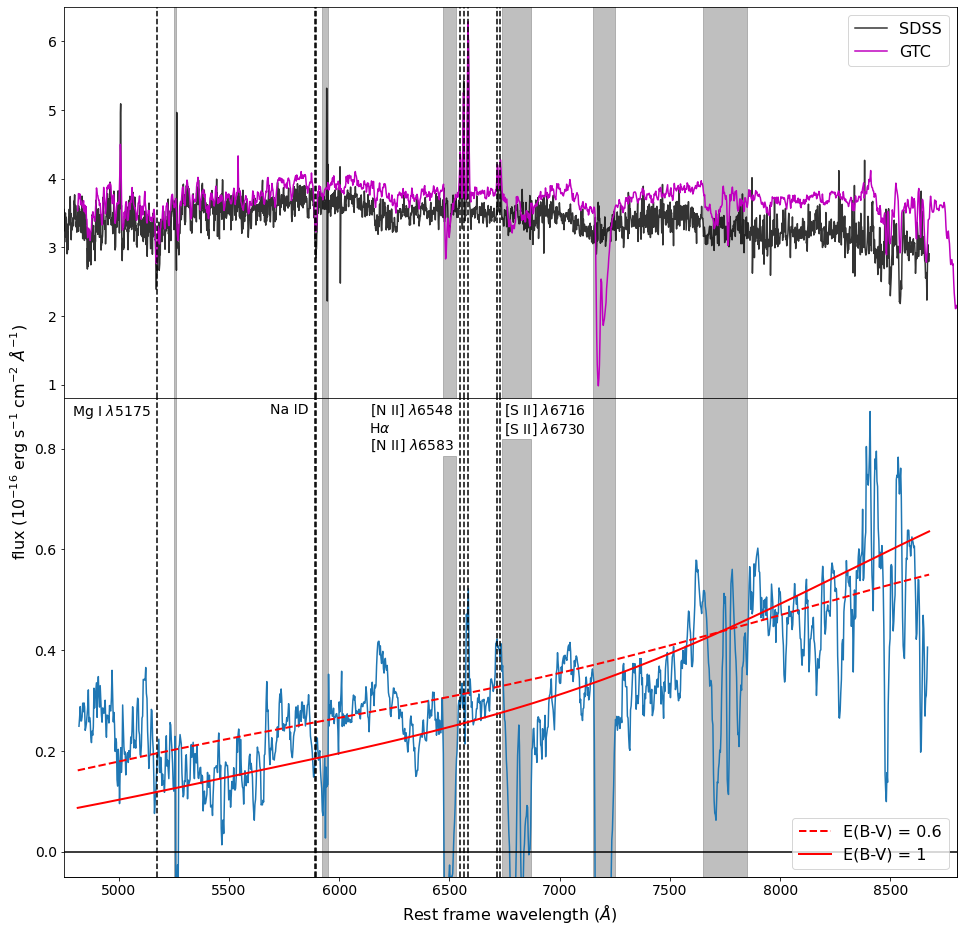
\includegraphics[width=\textwidth]{../Images/chapter_3/spec_obj.png}
 \caption{Spectrum of the late-time signal in SN 2020alm in its rest frame. The top panel shows the late-time spectrum obtained on 26 July 2023 using OSIRIS on the GTC, and the SDSS spectrum obtained in 2003. The bottom panel shows the late-time excess, obtained by subtracting the SDSS host galaxy spectrum from the observed late-time spectrum. A smoothed spectrum is shown in blue. The smoothing was done using a rolling kernel of size 5 to average over the values. The red lines are a simple TDE model with Milky Way and some amount of host galaxy extinction applied (the amount is shown in the legend), in order to get the approximate shape of the observed spectrum. Narrow emission and absorption lines that were notable in the unsubtracted spectrum are marked with dashed lines. The grey regions are affected by sky lines, and should be ignored. The late-time spectrum of SN 2020alm is available in electronic form at the CDS via anonymous ftp to \url{cdsarc.u-strasbg.fr} (130.79.128.5), via \url{http://cdsweb.u-strasbg.fr/cgi-bin/qcat?J/A+A/ }or upon request to the author.}
 \label{ZTF20aaifyfx_spec}
\end{figure}

\section{Binned SMP light curves of the final candidates}
\begin{figure}
 \centering
 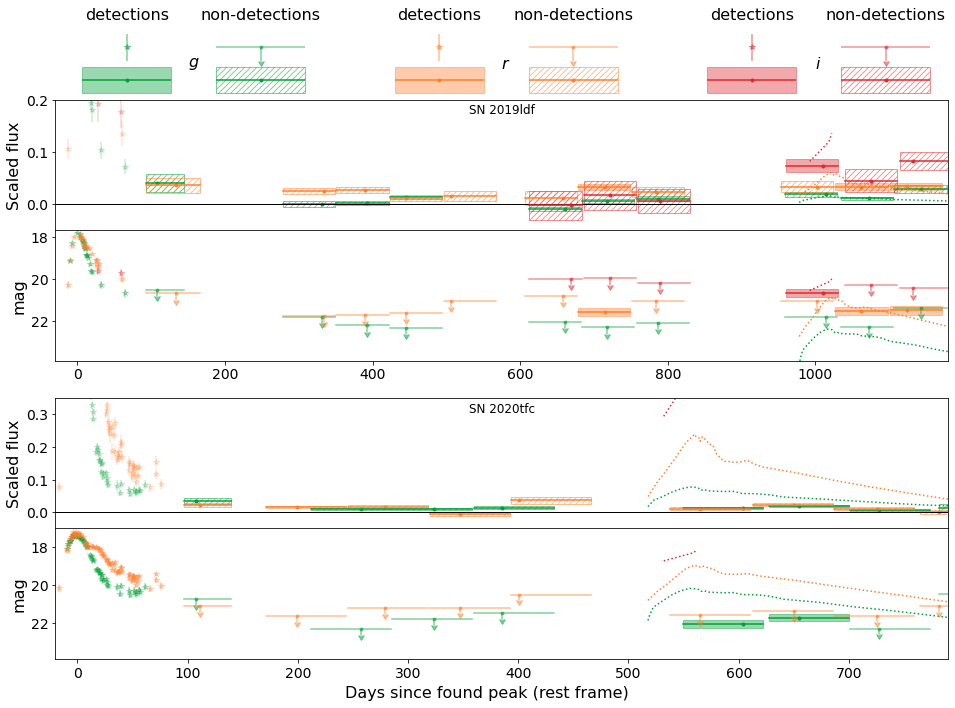
\includegraphics[width=\textwidth]{../Images/chapter_3/candid_plots_smp.png}
 \caption{Binned SMP light curves of the three candidate objects. As no bins $\geq5\sigma$ are recovered in SN 2018grt, it is not shown here. Both SN 2019ldf and SN 2020tfc do however still have robust detections in some bands. The best fitting alternate transients, shown in dotted lines, are the same as in Fig.~\ref{candidates}. The \ztfi-band of SN 2020tfc is not shown as the background was not subtracted completely, resulting in a significant flux offset.}
 \label{final_candid_SMP}
\end{figure}
\end{document}
%!TEX root = ../main.tex
\documentclass[a4paper,oneside,12pt, class=Latex/Classes/PhDthesisPSnPDF, crop=false]{standalone}
\usepackage{setspace}
\begin{document}
\doublespacing
\chapter{ZTF-observed late-time signals of pre-ZTF transients}
\label{chap:pre-ZTF_search}


In Chapter \ref{chap:DR2_search} I presented my pipeline to search for faint signals in light curves by binning observations together to push beyond the single observation magnitude limit. This pipeline was then used to search for signs of late-time CSM interaction in the ZTF SN Ia DR2 data set, finding three candidate objects in a sample of 3\,628 objects. For a late-time signal to be detected in this sample requires both the SN and the late-time signal to occur after the start of ZTF, which sets an age limit of at most 5.5 years on any theoretically identifyable CSM interaction.

However, the binning procedure does not rely on having the original SN as part of the light curve that is to be binned. As long as the coordinates of the SN are known a forced photometry light curve spanning the entire duration of ZTF can be constructed and put through the pipeline (although a slight modification of the baseline correction will be needed, see Section \ref{sec:Pipeline_modifications}). This means that by using SNe that exploded before the start of ZTF, much later epochs can be investigated for signs of late-time signals. On top of this, as most SNe are expected to have faded before the start of ZTF the procedure becomes identical for any type of transient, allowing me to widen my search beyond SNe Ia.

In Section~\ref{Pre-ZTF_data}, I build my sample of objects whose first detection was in the decade before the start of ZTF. In Section~\ref{Pre-ZTF_analysis}, I introduce the changes I made to the pipeline to adapt it to this sample, and the post-binning analysis. In Section~\ref{Pre-ZTF_results}, I describe the objects flagged by the binning program and split them into different groups with different origins. These are discussed in Section~\ref{Pre-ZTF_discussion}, and I conclude in Section~\ref{Pre-ZTF_conclusions}.

\color{red} This is Paper II, but needs to be properly adapted. All commented out sections are still in the overleaf version if needed. Copied starting from end of intro until the end of conclusions and put the appendices in their original location. To-do list: Check for broken references, check for double refs, reformat pages, make sure all the \ztfg\ztfr\ztfi\ things are consistent\color{black}


\section{Data}
\label{Pre-ZTF_data}
My first aim is to compile a list of all transients discovered in the decade before ZTF started. To build my sample, I started with all transients in the Open Supernova Catalog (OSC\footnote{\url{https://github.com/astrocatalogs/supernovae}}, \citealt{Open_SN_cat}) that were discovered between 1 January 2008 up to 1 January 2018, giving me 22\,790 objects. I end my sample a few months before the start of the full ZTF survey in March 2018 to remove most pre-ZTF transients that were still visible by the start of ZTF. For each object I require a name, sky position, redshift, and classification of its type. I require the redshift to make an informed estimation of the absolute luminosity of any potentially detected late-time signal. For the vast majority of transients, a classification means a spectrum was obtained that enabled typing but the size of the sample precludes checking of each individual classification. However, further investigation of identified interesting events is performed where required. I also include objects classified as a `SN candidate' as they are likely SNe but were never spectroscopically classified. These requirements cut my sample down to 8\,865 objects. By querying WISeREP\footnote{\url{https://www.wiserep.org}} \citep{wiserep} for objects reported in the same date range, I attempted to recover objects that were incomplete or absent from the OSC. Out of the 12\,955 OSC objects that did not have all the required information and no WISeREP match, 1\,137 had no sky position while the other 11\,818 had a sky position but no reported redshift and/or classification.

From the combined sample, I removed objects at Dec $\leq -32\deg$ as ZTF is unable to observe below Dec $\approx -30\deg$. After these updates (including WISeREP and with the Declination cut) my sample increased to 8\,914 objects. The declination cut is liberal to ensure all object locations that could have been observed with ZTF remain in my sample. Objects outside the ZTF footprint but still in my sample are cut automatically when obtaining the ZTF light curves. I do not make a cut on proximity to the host nucleus as I want to be as inclusive as possible. Instead I accept the possible contamination by nuclear activity which, as will be shown later, is in most cases easily identifiable.

While cross-matching between OSC and WISeREP to remove duplicate entries, I noted several objects with different names and discovery dates but located very close on the sky. While uncommon, it is not impossible for multiple SNe to occur at the same sky position in short succession. \citet{Terwel_2024_paper1} found several such sibling transients at very small separations where both SNe were detected by ZTF. Since I just look at the late-time light curve at the sky position of each pre-ZTF transient, sibling transients like these are investigated together as they have the sky position.

My late-time light curves at the position of each transient in the list were constructed, using the method detailed in Section \ref{Pre-ZTF_analysis}, between 9 December 2023 and 24 January 2024 using all available ZTF data at the time. This results in an effective range of over 5.5 years of ZTF observations for each object in my sample. For 207 sky positions that lay close to the edge of the ZTF survey, no ZTF observations were obtained and these were removed from my sample, leaving me with 8\,707 transients in my final sample. The ZTF light curves at these sky positions are generated using \textsc{fpbot}\footnote{\url{https://github.com/simeonreusch/fpbot}} \citep{fpbot}

I group the transients in my sample into one of nine classes based on the most precise common denominator of the reported classifications. For example, an object that was reported as both a SN Ia and SN Ib is grouped as a `SN I', and an object that was reported as some type of SN I and SN II is grouped as a `SN'. SLSNe are handled the same and grouped with normal SNe into SN I or SN II, though I can recover their SLSN classification if the object proves interesting later. Objects whose classification included the interacting classes SNe Ibn and SNe IIn are kept separately as I expect these may have a higher chance of having a late-time signature that can be picked up by ZTF. Figure~\ref{class_breakdown} shows the nine classes in my sample (`Ia', `II', `Ib/c', `IIn', `Ibn', `I', `SN', `SN candidate', and `not SN') and their relative sizes. 

For completeness I include a `non SN' class that consists of other types of transients. This class consists of 60 variable stars which include cataclysmic variables (CVs), luminous blue variables (LBVs), and novae, 36 nuclear transients (including TDEs and AGN), 73 other transients (including gap transients, impostor-SNe, kilonovae), and 140 Long Gamma Ray Bursts (LGRBs).
Figure \ref{class_hists} shows the amount of objects in each class as a function of redshift. My sample is biased towards lower redshifts as it is magnitude limited. I also have more objects that have been discovered in years where large surveys such as PTF, iPTF and ATLAS were active.


\begin{figure}
    \centering
    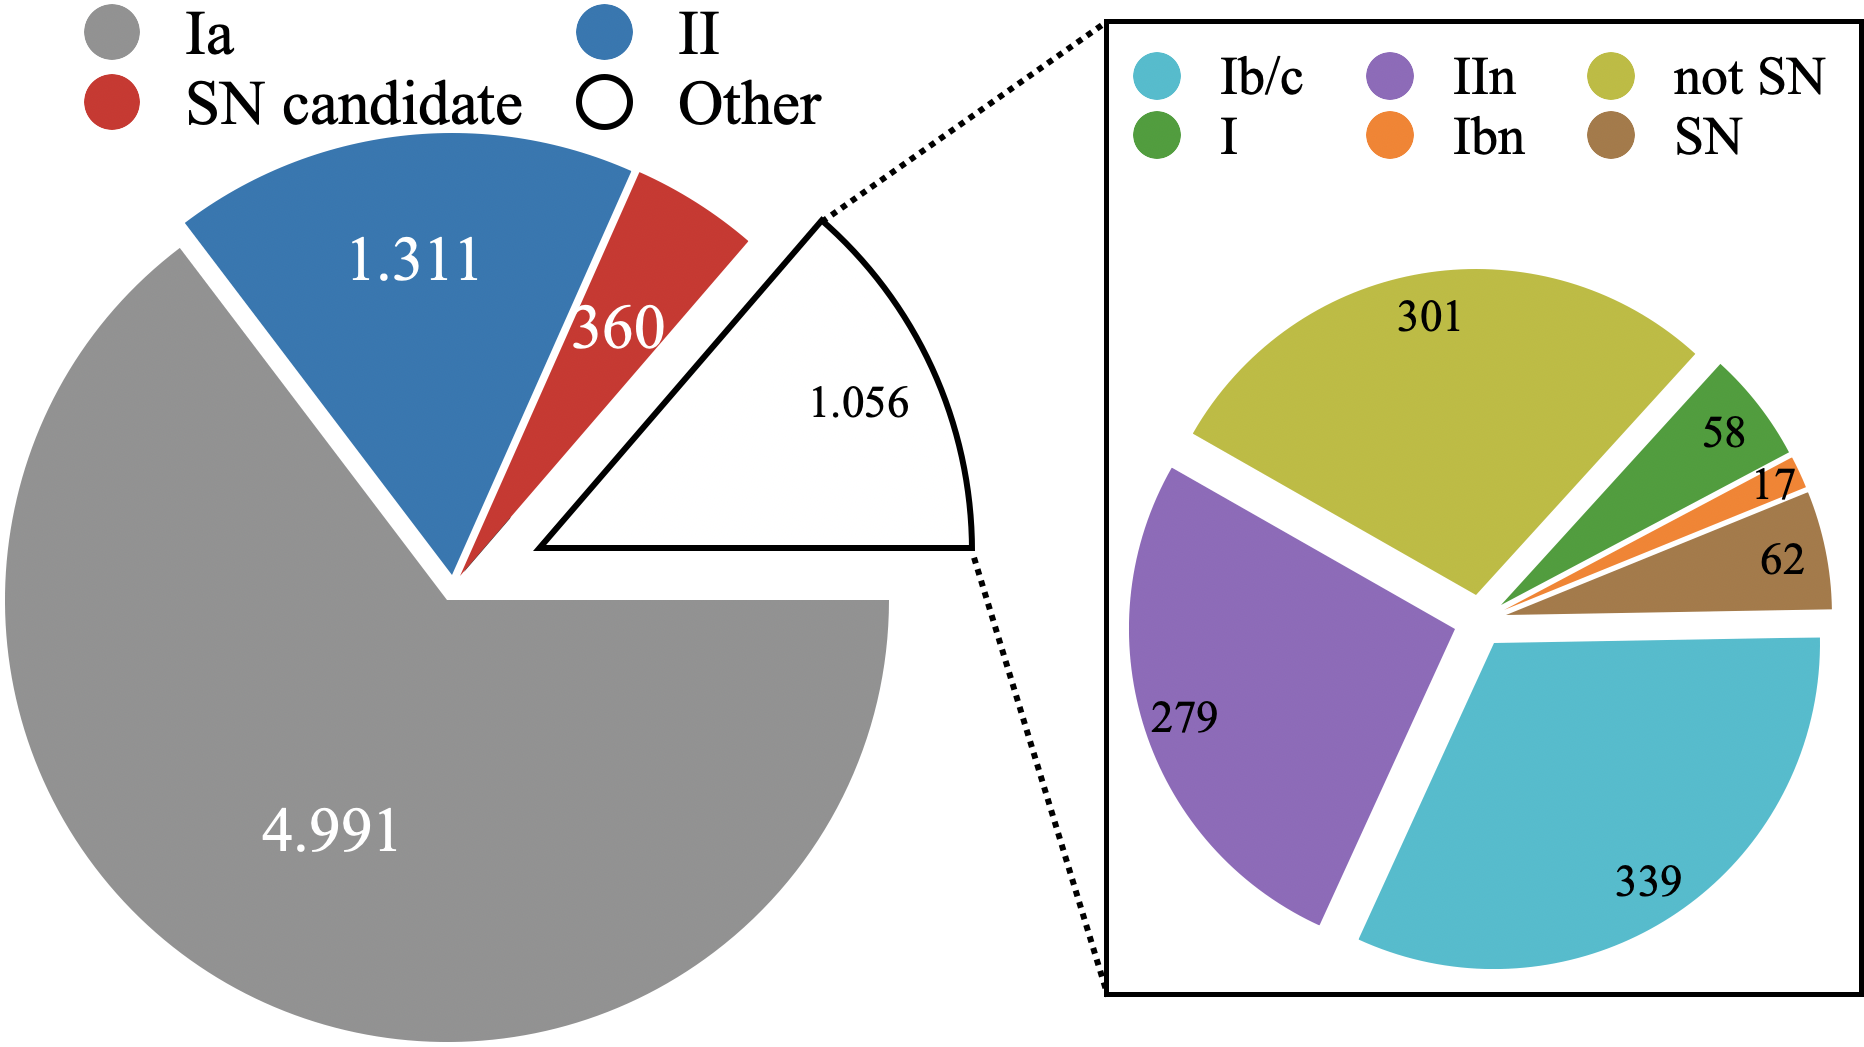
\includegraphics[width=\textwidth]{../Images/chapter_4/sample_pie.png}
    \caption{The final sample split into nine classes. As there is a big difference in class sizes, the smaller groups have been put together in the left chart as `other' and are split up in the right chart.}
    \label{class_breakdown}
\end{figure}


\begin{figure*}
    \centering
    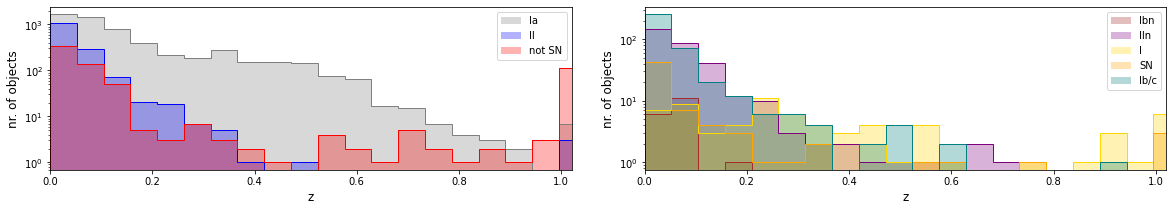
\includegraphics[width=\textwidth]{../Images/chapter_4/sample_hists.png}
    \caption{Sample size as a function of redshift for each class of objects. All objects with $z>1$ are put together in the bin starting at $z=1$. The histograms are split into two plots for better readability. In all classes of objects my sample is biased towards lower $z$.}
    \label{class_hists}    
\end{figure*}


\section{Analysis}
\label{Pre-ZTF_analysis}
I use an adapted version of the pipeline introduced in \citet{Terwel_2024_paper1} to test for late-time flux excesses in my sample of pre-ZTF transients. In brief, the pipeline first applies a baseline correction to ensure that the light curve has zero flux when no signal is expected \citep[e.g.][]{Yao_baseline_corr,Miller_baseline_corr}. It then bins the post-SN observations together in bins of 25, 50, 75, or 100 days to recover signals that are below the noise level of individual observations. To test if bin placement has an effect on the result, the binning is performed multiple times with shifted bin phase locations. Only signals that are sufficiently insensitive to bin placement are considered real. Binning observations increases the depth at which signals can be recovered at the cost of time sensitivity. As the smallest bins are 25 days in the observer frame, this means that I cannot detect details at similar or smaller time scales, such as rise times or short-term variations. In Section \ref{sec:Pipeline_modifications}, I describe the modifications of my detection pipeline from \cite{Terwel_2024_paper1}. In Section \ref{sec:false_positives}, I discuss the identification of false positives and in Section \ref{CSM_calc}, I describe a method of obtaining a rough estimate of potential CSM masses to explain any observed late-time signals.

\subsection{Detection pipeline modifications}
\label{sec:Pipeline_modifications}
My main modifications to the pipeline presented in \citet{Terwel_2024_paper1} are in the method of the baseline correction and the removal of the tail fitting procedure that was put in place to remove false positives from detecting the end of a normal SN Ia tail decline. In \citet{Terwel_2024_paper1} the baseline correction was done by using the pre-SN observations, as late-time signals are expected in the observations only after the SN explosion. This cannot be done in my current sample since the date of explosion is not contained within the ZTF data time frame. Instead, I have to consider that a period with flux excess could occur any time during the ZTF observations. 

Therefore, I run the pipeline several times using three different time frames for the baseline corrections. These time frames are chosen at the start, middle, and end of my ZTF light curves (see Table~\ref{baseline_regions}). I choose the baseline time frames to each be a year long to ensure that the targets are likely to have been observed, even if there are gaps in the observations due to the target location not being observable the entire year. I also choose not to include the first few months of ZTF data in the first baseline region as the final calibrations were not completed until July 2018 \citep{ZTF_overview_and_1st_results}. By using different baseline regions I ensure that I bin the entire light curve multiple times (since the region used for the baseline corrections cannot be included in the light curve binning). If one of the baseline regions overlaps with the late-time signal the result can be a false baseline correction. By using multiple baseline regions these cases can be more easily be identified. 

To ensure that there were enough points in each baseline region for a robust correction, I ignore all detections where the band in which the detection was found had $< 30$ points in the baseline. Table \ref{baseline_regions} shows the number of objects that meet this condition within each baseline region in each of the observational bands. In total, 989 objects never meet this condition in any band and are effectively removed from my sample, reducing the sample to 7718 objects.

A fitting procedure to identify the post-peak radioactive tail components of SNe Ia was used in \citet{Terwel_2024_paper1}. This was to distinguish between a normal SN Ia tail that was still visible $\sim$100 days after the peak when the binning started and detections that could not be attributed to the decay tail of a normal SN Ia. Since the sample in this paper consists of transients that were first detected and expected to have (mostly) faded before the start of ZTF, this procedure is not needed. Also, I do not restrict myself to just SNe Ia, but search for late-time signals in any transient discovered in the 10 years before the start of ZTF. Therefore, for example, a procedure trying to find a SN Ia tail in a SN II event will always fail to do so.


\subsection{Removing false positives}
\label{sec:false_positives}
The pipeline outputs a list of 504 objects that have $5\sigma$ or greater binned detections in a band in at least four out of 16 attempts (four bin sizes, each shifted four times to avoid spurious detections caused by specific bin placement, see \citealt{Terwel_2024_paper1} for more details). These are inspected visually to determine if the detections are due to observational issues, software issues, or if it is likely astrophysical in nature. A large fraction of the flagged light curves were deemed false positives after visual inspection. The main causes of the binning program wrongly finding bins with detections are due to issues in the difference imaging processing or the baseline correction.

To investigate these cases, I use the SuperNova Animation Program (\textsc{snap}\footnote{\url{https://github.com/JTerwel/SuperNova_Animation_Program}}) to inspect the difference images directly. Details on \textsc{snap} are presented in \citet{Terwel_2024_paper1}. Many false positives are identified as due to being close to another source by inspection of the difference images. Usually this other source is the host galaxy (nucleus) but in some cases it can also be a foreground star. This can lead to an issue with an improper subtraction of the bright source, which results in a residual, generally a dipole, at the position that is picked up by my pipeline. To identify these cases, I use \textsc{snap} to visually inspect the images and remove spurious detections. This removes 155  events from my sample. 

The other main group of false positives (88 cases) are flagged due to issues in the baseline determination. These can present as extremely large corrections, in some cases several orders of magnitude larger than the signals I expect to find. A baseline correction of $\mathcal{O}(10^5)$ can make a 17.5 mag signal appear or disappear. While in some cases big corrections are needed (see Section~\ref{tails}) in most cases such a correction led to noisy light curves, preventing me from probing beyond the individual ZTF image mag limit. In other cases the baseline is not constant but seems to vary over time or suddenly jump, making it very difficult or impossible to apply a proper baseline correction.

One potential cause of these issues could be due to ZTF continuing to improve the reference images by rebuilding them and stacking more observations, including observations from during the survey \citep{ZTF_Instrumentation}. To be able to compare observations from before and after this is done, one should remake all the difference images using the updated references. However, this is not feasible in a survey as large as ZTF, and since the offsets are usually below the noise threshold of the individual images the issue is of little importance to most of the survey science outputs. Only when attempting to go beyond the single image noise limit using, for instance, my binning method, this issue becomes noticeable enough and can lead to baseline offsets and varying or jumping baselines.

In 19 cases there were enough points in the baseline for the object to stay in my sample but the light curve was sampled sparsely with large gaps without observations surrounding sparse detections, making it impossible to determine the validity of these detections as there are no proper non-detections close in time to compare against.


\begin{table}[]
    \centering
    \caption{Details of the three baseline regions used in my pipeline. The first column gives the start and end MJD of each baseline region, and the second column gives its length in days. The last three columns give the number of transients that had at least 30 points in the baseline to provide a robust estimate of the baseline, in the \textit{g}, \textit{r}, and \textit{i} band, respectively}
    \begin{tabular}{ccccc}
        \hline
        \hline
        Baseline region & Length (d) & \multicolumn{3}{c}{No. passing cuts} \\
        (MJD)&& \ztfg & \ztfr & \ztfi \\
        \hline
        58300 -- 58664 & 365 & 6817 & 7198 & 744\\
        59031 -- 59395 & 365 & 7251 & 7258 & 3447\\
        59915 -- 60335 & 422$^*$ & 4792 & 5350 & 2457\\
        \hline
    \end{tabular}
    \label{baseline_regions}
\begin{flushleft}
    $^*$ The light curves were generated between 9 December 2023 and 24 January 2024, meaning that the final baseline for each object is between 374 and 420 days long. The final two days are a buffer to ensure all data is used.
\end{flushleft}
\end{table}


\subsection{Estimating CSM masses}
\label{CSM_calc}
In Sect.~\ref{weirdo_section}, I describe my final shortlist of late-time flux excesses that cannot be explained by other sources. To determine if they are potentially due to CSM interaction signatures, I can make a rough estimate of the CSM mass required to generate such a signal. In this section, I describe the method used by \citet{2015cp} to put constraints on the CSM mass of their targeted SNe at similar epochs to mine, based on the observed near-ultra-violet (NUV) (non-)detections using the models of \citet{CSM_models_Harris}. While CSM is line dominated, especially bye \Halpha, it is much more difficult to estimate a CSM mass without making many assumptions about the state of the CSM. Even though the statistical errors can be large, the resulting CSM masses for some of the objects in Sect.~\ref{weirdo_section} is still unreasonable.

Assuming that the time of the late-time detections correspond to the peak of the CSM interaction light curve, \citet{2015cp} showed that the Bremsstrahlung spectral luminosity $L_\nu$ at frequency $\nu$ at the moment the interaction shock reaches the outer edge of the shell is
\begin{equation}
    \label{15cp_L_nu}
    L_\nu \approx 1.63 \times 10^{-31} T^{-1/2} t_r^{-3} M_\text{CSM}^{17/7} \text{e}^{-\frac{h\nu}{kT}} y(F_R) \text{ erg s}^{-1},
\end{equation}
where $T$ is the temperature of the shocked material in Kelvin, $t_r = t/(1+z)$ is the time after explosion in seconds in the rest frame of the SN at which the ejecta reach the outer edge of the CSM shell and the interaction is assumed to be at its strongest, $M_\text{CSM}$ is the CSM mass in grams, and $y(F_R) = F_R^{-3/7}(1-F_R^{-3})^{-10/7}$ is the dependence on the fractional radius of the shell $F_R \equiv R_\text{out} / R_\text{in}$. Here $R_\text{out}$ and $R_\text{in}$ are the outer and inner radius of the CSM shell, respectively. $F_R = 1.1$ represents a thin nova-like shell, with higher values representing thicker shells. This equation assumes a low density, fully ionized H-dominated CSM to be the emission source after the interaction. 

\citet{2015cp} derive Eq.~\ref{15cp_L_nu} to use in the NUV and assume temperatures around $10^8$~K. In these conditions the exponential term is near unity and can be ignored. Since I am targeting optical wavelengths, if the mechanism described here is the source, lower temperatures are needed where the exponential term cannot be ignored. The other assumptions made in \citet{2015cp} still hold for optical wavelengths, so I can use Eq.~\ref{15cp_L_nu} to estimate the $M_{CSM}$ required to explain any detected late-time signals using
\begin{equation}
    \label{mag_lum_rel}
    10^{-0.4M} = \frac{L}{L_0} = \frac{L_\nu c}{L_0 \lambda},
\end{equation}
with $M$ the absolute magnitude of the detected signal, $c$ the speed of light, $L_0 = 3.0128 \times 10^{35}$ erg s$^{-1}$ the zero point luminosity, and $\lambda$ the effective wavelength of the band I am considering ($4\,746.48$ \AA, $6\,366.38$ \AA, and $7\,829.03$ \AA~for \textit{g}, \textit{r}, and \textit{i}, respectively). By combining Eq.~\ref{15cp_L_nu} and Eq.~\ref{mag_lum_rel} I get
\begin{equation}
    \frac{M_\text{CSM}}{M_\odot} \approx 3 \times 10^{-8-\frac{14}{85}M} \left(\frac{T}{\text{K}}\right)^{\frac{7}{34}} \left(\frac{t/(1+z)}{\text{days}}\right)^{\frac{21}{7}} \left(\frac{\lambda}{\text{\AA}}\right)^{\frac{7}{17}} \text{e}^{\frac{7hc}{17kT\lambda}} y(F_R)^{\frac{-7}{17}}.
    \label{M_CSM_eq}
\end{equation}
I can obtain $M$, $t$, and $z$ directly from my shortlist of transients with potential CSM interaction. For $t$ the start of the signal should be taken as this assumes the least delay due to a non-negligible light-crossing time across the CSM shell. The remaining parameters are the fractional radius of the shell and the temperature.

If I assume the CSM shell to be nova-like then $F_R=1.1$. Equation~\ref{M_CSM_eq} gives very massive CSM shells very easily, especially if a significant delay time before the onset of the CSM interaction is present. The required $M_\text{CSM}$ can be somewhat lowered if I assume that the actual thickness $R_\text{in} - R_\text{out}$ of the CSM shell remained constant after its creation, meaning that $F_R$ decreases as the shell travels outwards. Since the SN ejecta move at a constant velocity, the distance of the CSM is proportional to the delay time of the interaction signal. If I assume a shell with $F_R = 1.1$ has a radius if the late-time signal occurs at 300 days after the explosion, that same shell will have $F_R \approx 1.01$ if the interaction starts 3000 days after the explosion. I assume temperatures of 10$^5$ to 10$^7$ K, lower than the value assumed by \cite{2015cp} of 10$^8$ K, but more suitable for explaining optical emission.

In Section \ref{weirdo_section}, I discuss the results of the CSM mass estimate for events with late-time flux excesses to determine if CSM interaction could be a plausible explanation. Equation~\ref{M_CSM_eq} assumes that the magnitude is corrected for extinction. To get the lowest $M_\text{CSM}$ possible I assume there is only Milky Way extinction in the line of sight of any of my targets. Any extinction in the host galaxy would make the intrinsic colour of these objects bluer allowing for higher temperatures, but also raise the intrinsic absolute magnitude resulting in a higher overall estimate for $M_\text{CSM}$. The estimates should therefore be seen as lower limits.


\section{Results}
\label{Pre-ZTF_results}
I have identified 98 transients with potential late-time excesses in their light curves that require further investigation. In Section~\ref{tails}, I describe the group of objects whose detections in ZTF can directly be linked to the pre-ZTF transient. These transients were still bright enough at the start of the ZTF survey to be detectable. In Section~\ref{siblings}, I describe objects whose found ZTF signal is due to a sibling transient occurring at nearly the exact same sky position. A small fraction of my sample consists of non-SN transients, a few of which are returned by the pipeline and these are discussed in Section~\ref{non-sn}. Finally in Section~\ref{weirdo_section}, I describe the objects that required an individual, deeper investigation of the signal found in ZTF.


\subsection{Pre-ZTF transients still active in ZTF}
\label{tails}
I chose to limit my sample to those objects that were first detected before 2018 to reduce the number of transients still visible at the start of ZTF. While this three month gap is enough for most transients to fade away, some super-luminous SNe, Type II-Plateau SNe, interacting classes like SNe Ibn and IIn, and even very nearby SNe Ia that exploded before ZTF started, may still be active during the ZTF survey time frame.

\begin{figure*}
    \centering
    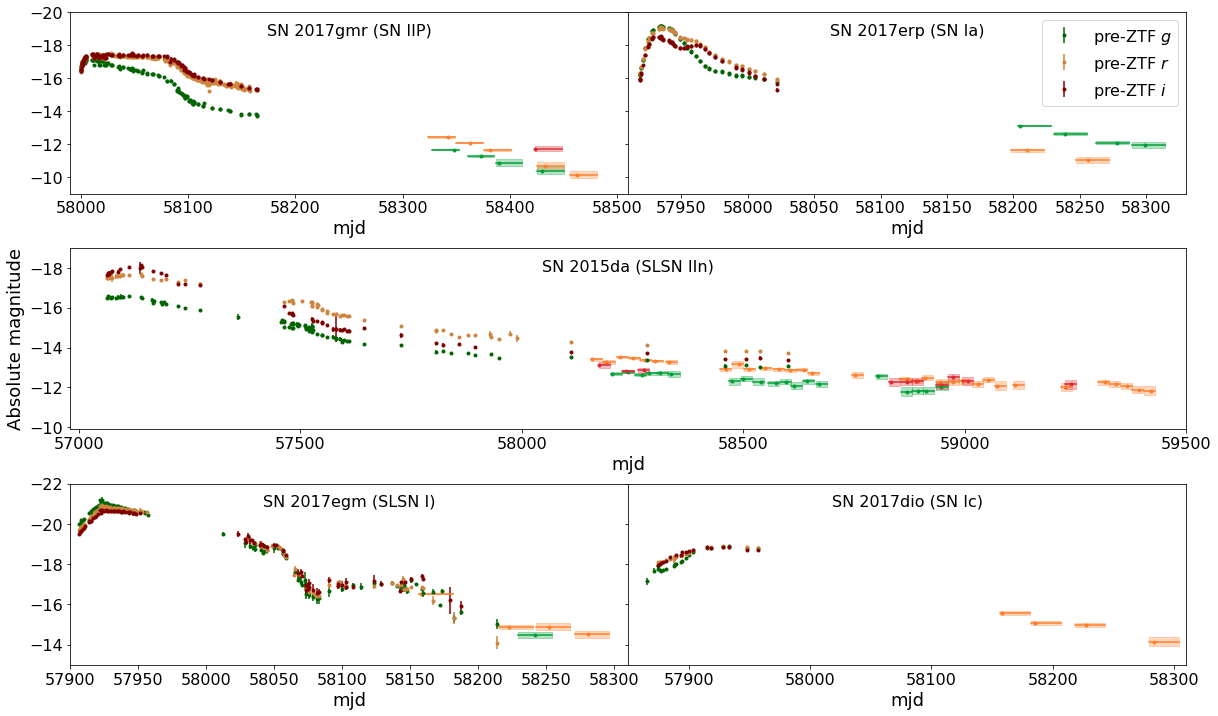
\includegraphics[width=\textwidth]{../Images/chapter_4/tails.png}
    \caption{Examples of pre-ZTF SNe whose light curves have been recovered in the binned ZTF light curves. For each object I show the pre-ZTF \ztfg~(dark green), \ztfr~(dark yellow), and \ztfi~(dark red) data points, as well as the binned ZTF detections (green, orange, red, respectively). The binned ZTF observations are in 25 day bins, with the width showing the beginning and end of each bin, and the shaded region shows its $1\sigma$ magnitude uncertainty. The pre-ZTF data was taken from \citet{2017gmr} (SN 2017gmr), \citet{2017erp} (SN 2017erp), \citet{2015da_2020} (SN 2015da), \citet{2017egm} (SN 2017egm), and \citet{2017dio} (SN 2017dio). None of the light curves are corrected for host extinction.}
    \label{tail-examples}
\end{figure*}

As these objects were active while the initial set of ZTF reference images were being produced, none of these objects have been found by ZTF even when the SN was still bright enough to be detected by ZTF once observing began. As the transient is in the reference images, it will cause an over-subtraction and leave an imprint, or ghost, at its location in the difference images. These are easily recognisable through visual inspection of the difference images using \textsc{snap}. Another clear sign is a significant baseline correction that is consistent between the different baseline regions after the transient has faded away. The baseline correction corrects for the flux offset the ghost creates, revealing the tail as observed by ZTF in the light curve.

I find 63 transients whose ZTF detections are consistent with on-going transient flux. These are listed in Table~\ref{tail_objects} and some example light curves are shown in Fig.~\ref{tail-examples}. The light curves show pre-ZTF data taken from the literature for  SN 2017gmr \cite[][]{2017gmr},  2017erp \cite[][]{2017erp}, SN 2015da \cite[][]{2015da_2020}, SN 2017egm \cite[][]{2017egm}, and SN 2017dio \cite[][]{2017dio}. SN 2015da is an extremely slowly declining SLSN IIn event \citep{2015da_2020, 2015da_2024} and its light curve extends in the binned ZTF data to approximately eight years after discovery. In SN 2015da, the pre-ZTF and binned ZTF light curves do not overlap exactly in magnitude at epochs when data from the different surveys are available (MJD 58300 -- 58600), showing that my pipeline underestimates the brightness of the transient. This is because some SN flux is still present even in my latest baseline region during mainly 2023, as can be seen in the observations presented in \citet{2015da_2024}. Therefore, the baseline correction is too small causing the binned detections to be slightly too low.

\begin{longtable}{ccccc}
\caption{List of the 63 pre-ZTF objects whose tail is still visible in ZTF using my binning method after a baseline correction.}
 \label{tail_objects}
 \endfirsthead
 \hline
 \hline
 Name &  Type & $z$ & Discovery date & visible until (mjd) \\
 \hline
 \endhead
 \hline
 \endfoot
 \hline
 \endlastfoot
 \hline
 \hline
 Name &  Type & $z$ & Discovery date & visible until (mjd) \\
 \hline
 AT 2017fwg & Candidate & 0.113627 & 01-08-2017 & 58325 \\
 AT 2017gpv & Candidate &  0.025563 & 04-09-2017 & 59480\\
 AT 2017gpy & Candidate & 0.025187 & 04-09-2017 & 58250 \\
 AT 2017hat & Candidate & 0.020454 & 01-10-2017 & 58275 \\
 AT 2017igk & Candidate & 0.040847 & 16-11-2017 & 58250 \\
 AT 2017ihh & Candidate & 0.027521 & 03-10-2017 & 58300 \\
 AT 2017iho & Candidate & 0.053421 & 17-11-2017 & 58250 \\
 AT 2017ims & Candidate & 0.030094 & 15-11-2017 & 58300 \\
 AT 2017iru & Candidate & 0.018156 & 29-11-2017 & 58375 \\
 ATLAS17nbe & Candidate & 0.013476 & 05-11-2017 & 58400 \\
 ATLAS17oai & Candidate & 0.099205 & 23-12-2017 & 58300 \\
 ATLAS18eas & Candidate & 0.033103 & 30-12-2017 & 58325 \\
 ATLAS18mmr & Candidate & 0.077507 & 15-12-2017 & 58325 \\
 DES16X2bkr & SN II & 0.159 & 21-09-2016 & 58400 \\
 SN 2015da & SLSN IIn & 0.007222 & 09-01-2015 & 59475 \\
 SN 2016bkv & SN II & 0.002 & 21-03-2016 & 58475 \\
 SN 2016cyi & SN IIn & 0.044 & 25-06-2016 & 58475 \\
 SN 2016ieq & SN IIn & 0.066 & 14-11-2016 & 58400 \\
 SN 2017aym & SN IIP & 0.005928 & 13-01-2017 & 58700 \\
 SN 2017dio & SN Ic & 0.037 & 26-04-2017 & 58300 \\
 SN 2017dpu & SN II & 0.018 & 30-04-2017 & 58250 \\
 SN 2017eby & SN Ia-CSM & 0.081 & 01-04-2017 & 58350 \\
 SN 2017egm & SLSN I & 0.030721 & 23-05-2017 & 58300 \\
 SN 2017emq & SN Ia & 0.005247 & 03-06-2017 & 58250 \\
 SN 2017erp & SN Ia & 0.006174 & 13-06-2017 & 58375 \\
 SN 2017err & SLSN IIn & 0.107 & 12-06-2017 & 58275 \\
 SN 2017faa & SN II & 0.01845 & 27-06-2017 & 58300 \\
 SN 2017fgc & SN Ia & 0.007722 & 11-07-2017 & 58400 \\
 SN 2017fvr & SN IIP & 0.012539 & 01-08-2017 & 58450 \\
 SN 2017gas & SN IIn & 0.011 & 10-08-2017 & 58850 \\
 SN 2017ghw & SN IIn & 0.076 & 25-08-2017 & 58450 \\
 SN 2017glx & SN Ia-91T & 0.011294 & 03-09-2017 & 58400 \\
 SN 2017gmr & SN IIP & 0.005037 & 04-09-2017 & 58475 \\
 SN 2017gvb & SN IIn & 0.030344 & 18-09-2017 & 59000 \\
 SN 2017gww & SN II & 0.01748 & 26-09-2017 & 58375 \\
 SN 2017gxq & SN Ia & 0.008406 & 17-09-2017 & 58450 \\
 SN 2017hcc & SN IIn & 0.0173 & 02-10-2017 & 58500 \\
 SN 2017hbg & SN II & 0.016 & 25-09-2017 &  58375\\
 SN 2017hca & SN II & 0.013403 & 28-09-2017 & 58450 \\
 SN 2017hfv & SN Ia & 0.028199 & 10-10-2017 & 58200 \\
 SN 2017hix & SN Ic & 0.012 & 13-10-2017 & 58375 \\
 SN 2017hlt & SN Ia & 0.027 & 10-10-2017 & 58275 \\
 SN 2017hmi & SN Ia & 0.0398 & 18-10-2017 & 58250 \\
 SN 2017hpa & SN Ia & 0.015654 & 25-10-2017 & 58400 \\
 SN 2017hqj & SN IIP & 0.009 & 27-10-2017 & 58300 \\
 SN 2017hro & SN II & 0.015 & 28-10-2017 & 58800 \\
 SN 2017igf & SN Ia & 0.005624 & 12-11-2017 & 58350 \\
 SN 2017ijr & SN Ia & 0.04 & 20-11-2017 & 58300 \\
 SN 2017ijx & SN Ia & 0.027729 & 18-11-2017 & 58300 \\
 SN 2017ivh & SN II & 0.008 & 05-12-2017 & 58300 \\
 SN 2017ivu & SN IIP & 0.006528 & 11-12-2017 & 58400 \\
 SN 2017ivv & SN II & 0.022 & 12-12-2017 & 58450 \\
 SN 2017ixg & SN Ia & 0.0277 & 14-12-2017 & 58400 \\
 SN 2017ixv & SN Ic-BL & 0.007302 & 17-12-2017 & 58350 \\
 SN 2017ixx & SN II & 0.041 & 17-12-2017 & 58300 \\
 SN 2017ixz & SN IIb & 0.024 & 14-12-2017 & 58250 \\
 SN 2017iyd & SN IIb & 0.0285 & 13-12-2017 & 58275 \\
 SN 2017jav & SN Ia & 0.01517 & 19-12-2017 & 58275 \\
 SN 2017jbj & SN II & 0.013492 & 20-12-2017 & 58400 \\
 SN 2017jeh & SN Ia & 0.020961 & 26-12-2017 & 58275 \\
 SN 2018L & SN Ia & 0.02582 & 25-12-2017 & 58325 \\
 SN 2018bq & SN Ia & 0.025628 & 30-12-2017 & 58275 \\
 SN 2018fd & SLSN I & 0.263 & 11-10-2017 & 58450 \\
\end{longtable}


\subsubsection{AT 2017gpv - a 14hls-like event}
\begin{figure*}
    \centering
    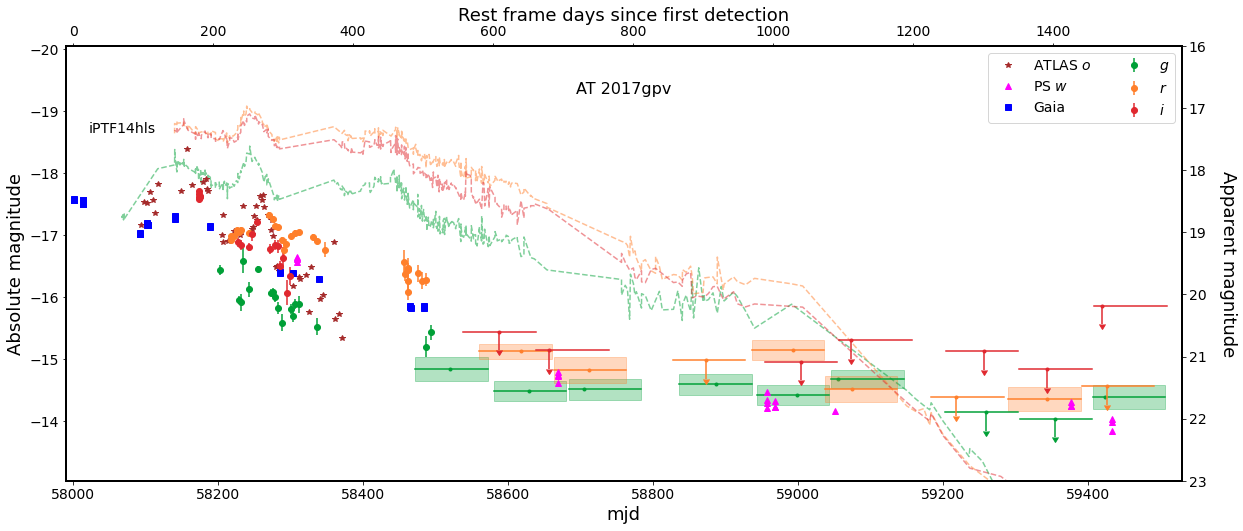
\includegraphics[width=\textwidth]{../Images/chapter_4/17gpv.png}
    \caption{Light curve of AT 2017gpv with the axes representing absolute magnitude (left), apparent magnitude (right), the rest frame days since first detection (top) and mjd (bottom). Single epoch detections by ZTF, Gaia, Pan-STARRS and ATLAS are shown, as well as the binned ZTF observations after the transient faded below the single epoch noise limit. The dashed lines are the \textit{gri}-band light curves of iPTF2014hls, which have been corrected for time dilation but not extinction (data taken from \citealt{iPTF14hls_Iair, Sollerman_2019_iptf14hls}).}
    \label{17gpv_plot}
\end{figure*}

AT 2017gpv, shown in Fig.~\ref{17gpv_plot}, is an unusual event similar in nature to iPTF14hls \citep{iPTF14hls_Iair, Sollerman_2019_iptf14hls} and SN 2020faa \citep{Yang_2021_20faa} that was detected by my pipeline in the ZTF data. It was originally identified by Gaia, which detected it repeatedly during the first 500 days after its discovery. It has also been detected by ATLAS, which has a rich $o$-band light curve between 100 and 300 days after discovery that shows a plateau followed by a shallow decline that is interrupted by a rebrightening event. The first detections in ZTF are visible even in the non-binned data beginning around 200 days after first detection and lasting for around 400 days. With the binned observations the object can be recovered for another 1000 days before it fades below the noise limit. Pan-STARRS also detected this object in the $w$ band, and given its deep detection limits it detected the transient up to over 1400 days after discovery.

Due to the long duration of detections of AT 2017gpv in ZTF, only the last baseline region can be trusted as it has the least contribution from the late-time signal, though given the slow decline of the transient it is likely that there could still be some excess present at the time of the last baseline region. As expected, the baseline corrections are significant, and \textsc{snap} clearly shows the transient in the reference images, as well as a significant ghost in all difference images. While it was picked up by the ZTF alert system and given an internal name (ZTF18acueiall), it was not recognized as a real transient.

Unfortunately, AT 2017gpv was never spectroscopically classified. The transient is at a distance of 6.88$\arcsec$ from the host nucleus, removing host variability as a possible explanation, as well as limiting the amount of host extinction expected. The long time it was detectable and the bumpy nature of its light curves look similar to iPTF14hls \citep{iPTF14hls_Iair,Sollerman_2019_iptf14hls}, a very peculiar SN II that is also shown in Fig.~\ref{17gpv_plot}. Some similar events to iPTF14hls have been identified but they are rare \citep{Yang_2021_20faa, Soraisam_2022}. The light curve of iPTF14hls spans over 600 days and is very bumpy. In both cases the explosion epoch is badly constrained, but the peak found in iPTF14hls matches up quite well with the bump around MJD 58250 in AT 2017gpv. Overall, AT 2017gpv looks like a fainter and somewhat faster decaying version of iPTF14hls. The late-time data of iPTF14hls \citep{Sollerman_2019_iptf14hls} extends to $\sim$1200 d after discovery and shows a sharp decline after $\sim$1000 d, which is not seen in AT 2017gpv.

iPTF14hls is in my initial sample, but was not detected in ZTF because it is $\sim1000$ days older than AT 2017gpv. Assuming that these two events evolved in a similar manner, iPTF14hls would have been close to the detection limit at the start of ZTF and faded below that before it could be picked up by my pipeline.


\subsection{Siblings}
\label{siblings}
Siblings are two (or more) transients that occur in the same host galaxy. While siblings can occur at any location in a galaxy \citep[see e.g. ][for a sample of ZTF-detected siblings]{BTS_siblings, DR2_siblings}, a subset of these occur with a small enough sky separation that part of the light of one sibling can be detected when performing forced photometry at the sky position of the other sibling. In \citet{Terwel_2024_paper1}, five such sibling pairs were found, with both transients detected within ZTF. With my current sample being larger and spanning a bigger time range over which the second transient can be observed, it is reasonable to expect a larger number of same-location sibling transients. I arbitrarily define siblings as a transient detected in ZTF \textit{without} the use of additional binning to push the detection limit that are distinctively separate in time from the pre-ZTF transient at the same sky location. The ZTF transients do not have to be classified. I find 12 pairs of transients that satisfy these conditions, which I verified through the Fritz broker \cite{skyportal2019, Skyportal}. These are shown in Table~\ref{sibling_table}. 

\begin{table*}
    \centering
    \caption{Pre-ZTF transients with a sibling transient detected in ZTF in single exposures. The first four columns give the name, type, discovery mjd, and redshift of the pre-ZTF transient, and the next five columns give the same information of its ZTF sibling when available. The second to last columns gives an estimate of the peak \ztfr-band (unless specified otherwise) absolute magnitude of the ZTF transient assuming the pre-ZTF transient redshift, except for AT 2018iml as this is likely a foreground CV. The last column gives the separation between the siblings. A ? type means the transient was never spectroscopically classified. IAU names in parentheses are ZTF transients wrongly associated with a pre-ZTF transient.}
    \resizebox{\textwidth}{!}{
    \begin{tabular}{cccc|cccccc}
        \hline
        \hline
        \multicolumn{4}{c|}{Pre-ZTF transient} & \multicolumn{6}{c}{ZTF transient}\\
        Name & Type & MJD & Redshift & ZTF name & IAU name & Type & MJD & Peak mag & Sep ($\arcsec$)\\
        \hline
        AT 2017gcd & $^*$? & 57968 &0.028593 & ZTF19acdgwhq & SN 2019aavr & Ia-norm & 58763 & $-$18.8 & 1.02\\
        AT 2017keg & $^*$? & 58068 & 0.05 & ZTF19acihgng & SN 2019tka & Ia-norm & 58781 & $-$19.1 $^{(g)}$ & 1.69 \\
        SN 2013ld & $^*$? & 56522 & 0.02741 & ZTF18abavruc & SN 2021rgw & Ia & 59393 & $-$18.9 $^{(g)}$ & 0.57 \\       ASASSN-14ba & Ia pec/91T & 56796 & 0.032668 & ZTF22aaawghw & AT 2022csd & II & 59629 & $-$16.8 & 1.29 \\
        SN 2017acp & II & 57785 & 0.0215 & ZTF19aavqics & SN 2019gxo & II & 58633 & $-$18.1 & 3.15 \\
         SN 2014gz & II & 56678 & 0.02558 & ZTF21abcpbqd & SN 2021nof & II & 59362 & $-$17.2 $^{(i)}$ & 0.30 \\
        SN 2009hz & II & 55046 & 0.0253 & ZTF18acotwcs & AT 2018iml & CV?$^{**}$ & 58439 & -- & 0.33\\%
 iPTF15wk & Ia & 57097 & 0.23 & ZTF21aaeebxm & - & ? & 59226 & $-$20.0 $^{(g)}$ & 0.31 \\
        SN 2016bsc & Ia & 57500 & 0.05 & ZTF23aaeljse & (SN 2016bsc) & ? & 60043 & $-$17.9 & 1.61 \\
    
        SNF20080522-001 & Ia & 54608 & 0.04872 & ZTF22aalbuig & AT 2022kuh & ? & 59724 & $-$17.3 & 1.64 \\
        PS15ctg & Ia & 57328 & 0.078 & ZTF22abamjrf & AT 2022rol & ? & 59806 & $-$18.7 & 1.03 \\
        
        iPTF15eot & II & 57357 & 0.039 & ZTF19aakvysq & AT 2019bll & ? & 58541 & $-$17.5 & 2.19 \\
        \hline
    \end{tabular}
    }
    \begin{flushleft}
        $^*$ Classified ZTF SNe that were wrongfully associated with the pre-ZTF name resulting in a mis-classification. The pre-ZTF transient itself was never actually classified In the cases of AT 2017keg and SN 2013ld. The case of AT 2017gcd / SN 2019aavr has been fixed on TNS.\\
        $^{**}$ Not officially classified but based on evidence gathered from the ZTF forced photometry light curve.\\
        $^{(g)}$ Peak absolute magnitude in the \ztfg\ band.\\
        $^{(i)}$ Peak absolute magnitude in the \ztfi\ band.\\
    \end{flushleft}
    \label{sibling_table}
\end{table*}

In three cases, the ZTF-detected transient was classified but mistakenly associated with a pre-ZTF transient in WISeREP or OSC that subsequently got the same classification. In the case of AT 2017gcd, a decaying transient was observed in four epochs of unforced Pan-STARRS photometry, spread out over 125 days. This is enough to conclude that the 2017 transient was real and likely some kind of SN, but not necessarily a SN Ia.

In the two other cases (AT 2017keg/SN 2019tka and SN 2013ld/SN 2021rgw), the pre-ZTF detections are spurious and are unlikely to be true sibling pairs. AT 2017keg was reported by ATLAS in 2019 \citep{2017keg_disc} when SN 2019tka was found. Due to SN 2019tka being close to the host nucleus, likely spurious detections from two years before were present in the ATLAS light curve, resulting in the automated discovery report stating the wrong discovery date. SN 2019tka was reported by ZTF \citep{2019tka_disc}, which did not have such earlier detections as it only started operating in 2018. SN 2013ld was reported in 2021 by Pan-STARRS1. Again, its sibling SN 2021rgw was on top of the host nucleus, which has had several epochs of minor variability. Even the internal ZTF name is from 2018, showing that ZTF also detected minor changes at the host nucleus location. When SN 2021rgw was found, ZTF issued an alert with the discovery date in 2021, resulting in SN 2021rgw \citep{2021rgw_disc} while Pan-STARRS1 used the first unforced detection epoch in 2013 as the discovery date, resulting in SN 2013ld \citep{2013ld_disc}.

For the other nine sibling pairs listed in Table \ref{sibling_table}, the pre-ZTF sibling has a classification (five SNe Ia and four Type II SNe) obtained at the time of discovery. Three of their paired ZTF siblings were spectroscopically classified as Type II SNe at the time of discovery in ZTF. For AT 2018iml, the sibling of Type II SN 2009hz, the ZTF detections were obtained in two periods (November 2018 and March 2024) and they are best matched to a CV. The remaining five had no ZTF-era classification. In some cases the ZTF sibling is close enough to get wrongly associated with the pre-ZTF sibling and obtain the same IAU name.

Assuming the five unclassified ZTF transients occurred in the same host galaxy as their classified sibling, I can use the known redshifts to estimate the absolute brightness of the unclassified transients and show that they are in the range of SNe and unlikely to be caused by late-time CSM interaction.
ZTF21aaeebxm is found around 1800 days after its sibling, iPTF15wk, was first detected, and has an inferred absolute \textit{g}-band magnitude of $-20.0$ at its peak at just 0.31$\arcsec$ from iPTF15wk. To get such a strong signal this long after the explosion would require an unreasonably large CSM and thin shell, making CSM interaction an unlikely explanation. Its location is consistent with its host nucleus making a nuclear transient origin likely.

For ZTF23aaeljse, ZTF22aalbuig, ZTF22abamjrf, and ZTF19aakvysq, their absolute peak magnitudes are in the range typical of SNe ($-$17.3 to $-$18.7 mag) and \textsc{snap} shows that there is a noticeable separation between the pre-ZTF and ZTF-detected signals (1.03 to 2.19$\arcsec$), disfavouring any explanation that would require the two events to be at the same spatial position, such as CSM interaction. The inferred CSM masses to explain these events in this way are also unrealistically high. Their locations are inconsistent with their host nuclei. Therefore, I conclude that a sibling transient, likely a unclassified SN, is the most plausible explanation for these events. 


\subsection{Non-SN sources of flux excesses in ZTF}
\label{non-sn}
I identify some late-time excesses at the positions of my sample that are astrophysical but are due to known AGN activity or due to stellar variability. Ten transients (listed in Table~\ref{non-transient_table}) in my sample have been found to have genuine long-term variability due to an AGN that lasts for the whole time period of ZTF and is picked up by my pipeline. In each case, the source is a known AGN (verified through cross-referencing with SIMBAD, ZTF, and checking the AGN criterion from \citealt{WISE_crit} using the \textit{Wide-field Infrared Survey Explorer} WISE \citealt{WISE}). Their light curves are shown in Fig.~\ref{non-transients_AGN}. While several of the pre-ZTF transients in this category have been classified as SNe II, some have high redshift, which suggests that these are AGN misclassified as SNe II.

\begin{table}
    \centering
    \caption{Pre-ZTF transients detected in the binned ZTF light curves due to AGN or variable star activity. The original type and $z$ values are as they were recorded on the OSC or WISeREP. The late-time type gives the reason for the ZTF detections.}
    \begin{tabular}{cccc}
        \hline
        \hline
        Name & Pre-ZTF type & $z$ & Late-time type\\
        \hline
        Gaia14adg & II & 0.154 & AGN\\
        SN 2016fiz & II & 0.05 & AGN\\
        SN 2017avb & II & 0.096 & AGN\\
        LSQ12biu & IIn & 0.136 & AGN\\
        SN 2017bcc & SLSN-II & 0.133 & AGN\\
        PSN J0151 $^{(1)}$ & SLSN-II?/AGN & 0.26 & AGN\\
        ATLAS17khl & AGN & 0.06 & AGN\\
        PS17bgm & AGN & 0.358 & AGN\\
        LSQ12ehj & AGN & 0.12 & AGN\\
        AT 2017kas & SN candidate & 0.031328 & AGN\\
        LSQ12fgx & Variable star & 0 & Variable star\\
        SNhunt44 & LRV? $^{(2)}$ & 0.0005864 & Variable star\\
        AT 2016ijb & SN candidate & $-$0.000781 & Variable star\\
        PTF10qpf & Variable star & 0 & Variable star\\
        \hline
    \end{tabular}
    \label{non-transient_table}
    \begin{flushleft}
        $^{(1)}$ PSN J0151 = PSN J01510869+3155215\\
        $^{(2)}$ Potential luminous red variable
    \end{flushleft}
\end{table}

\begin{figure}
    \centering
    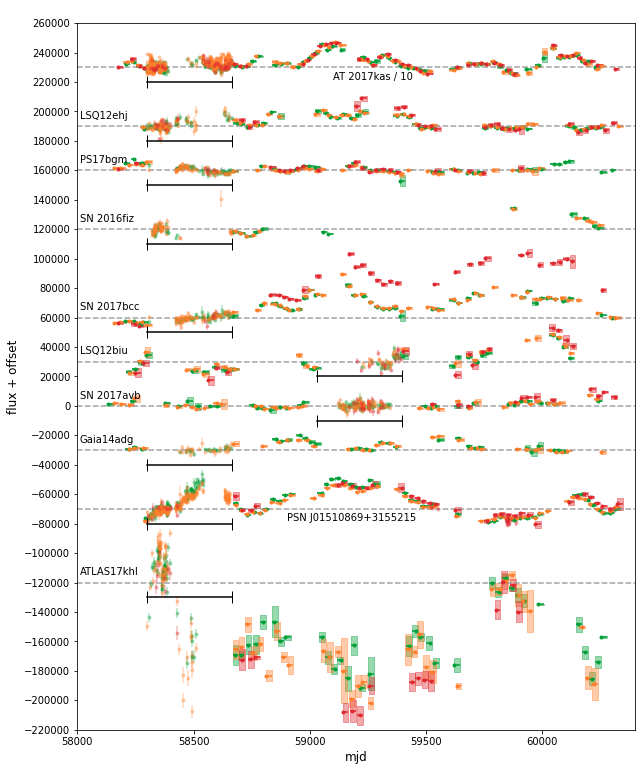
\includegraphics[width=0.9\textwidth]{../Images/chapter_4/non-transients_AGN.png}
    \caption{Binned flux of the recovered AGN. The flux is calibrated to a zeropoint at mag 30. The dashed lines show the baseline value for each object. Since the observations used to determine the baseline cannot be binned I show the unbinned data in the baseline region of each object, this region is marked by the black lines. Even though not all objects are properly sampled over the entire lifetime of ZTF, they all clearly show variability over long timescales. As these objects are always varying, it is impossible to do a baseline correction without the transient present. This causes some light curves to go below their baseline. Note that the values for AT 2017kas have been divided by 10 as the variability is so large.}
    \label{non-transients_AGN}
\end{figure}

\begin{figure}[h!]
    \centering
    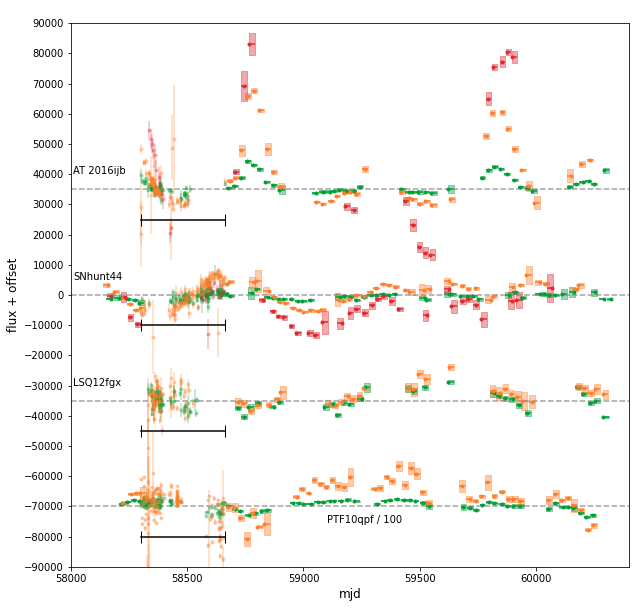
\includegraphics[width=0.9\textwidth]{../Images/chapter_4/non-transients_varstar.png}
    \caption{Binned flux of the recovered variable stars. The flux is calibrated to a zeropoint at mag 30. The dashed lines lines show the baseline for each object. Since the observations used to determine the baseline cannot be binned I show the unbinned data in the baseline region of each object, this region is marked by the black lines. All three objects vary around their central values, but the amplitude varies widely between the ZTF bands. Note that the values for PTF10qpf have been divided by 100 as the variability is so large.}
    \label{non-transients_varstar}
\end{figure}

I also recovered four long-term variable stars that are shown in Fig.~\ref{non-transients_varstar} and listed in Table~\ref{non-transient_table}. The nature of these sources make it impossible to create a template that always subtracts them completely without leaving residual flux or a ghost as there may be no region without variability. However, if the variations in the source's magnitude are large enough over a long period of time it will easily be picked up by the binning algorithm.


\subsection{Final shortlist of late-time interaction}
\label{weirdo_section}
The final 9 objects in my sample cannot be put in any of the groups (on-going SN flux, sibling transient, nuclear activity, variable star) above. Each of these events is discussed individually below. Table \ref{weirdos} shows the general information of these events, and their light curves are shown in Fig.~\ref{weirdo_plots}. The bin sizes and placement chosen for the plots are those that result in the clearest and cleanest signals. The baseline regions used are those that have the least amount of transient flux in them, which means they are the furthest away in time from the excess. As was done in \citet{Terwel_2024_paper1}, I compare the ZTF detections to several classes of transients in an attempt to explain them as a previously unidentified sibling transient. I also estimate the potential CSM mass required to explain the late-time signature using the analysis method detailed in Sect.~\ref{CSM_calc} for objects where a CSM interpretation cannot be ruled out.\\

\begin{sidewaystable*}
    \centering
    \caption{Objects with detections whose origin was not immediately clear. The first five columns give information on the original transient, and the last six columns give an overview of the binned ZTF detections. Start gives the time after discovery of the first detections in ZTF, and duration gives the length of these detections. Both are in rest frame days and rounded to 10 days. The \ztfg, \ztfr, and \ztfi\ columns give the range of detections in absolute magnitude if detected. Inferred cause of excess gives the type of object that best explains the detections. The last two columns state whether the excess is consistent with the SN and host nucleus location, respectively.}
    \resizebox{\textwidth}{!}{
    \begin{tabular}{ccccc|cccccccccc}
        \hline
        \hline
        \multicolumn{5}{c}{Pre-ZTF} & \multicolumn{6}{|c}{ZTF excess}\\
        \hline
        Name & Type & Discovery & $z$ & Host & Start & Duration & \ztfg\ band & \ztfr\ band & \ztfi\ band & Inferred & \multicolumn{2}{c}{Excess consistent with}\\
        && date && sep ($\arcsec$) & (d) & (d) & abs. mag & abs. mag & abs. mag & cause of excess & SN & host nucleus \\
        \hline
         SN 2017ige $^{(1)}$ &Ia & 17-11-17 & 0.02431 & 0.99 & 1190 $^{(2)}$ & 90 & $-$13.5 -- $-$13.3 & $-$14.3 -- $-$13.6 & -- & Sibling& yes & no \\
         SN 2016cob & Ia-91T & 26-05-16 & 0.02961 & 0.7 & 2200 & 490 $^{(3)}$ & $-$15.3 -- $-$14.7 & $-$16.5 -- $-$16.1 & $-$17.2 -- $-$16.4 & CSM/Nuclear& yes &yes\\
        SN 2017frh & Ia & 17-07-17 & 0.032188 & 0.0 & 250 $^{(2)}$ & 190 $^{(3)}$ & $-$15.6 -- $-$14.9 & $-$16.0 -- $-$15.6 & -- & CSM & yes & yes \\
        SN 2017fby & Ia & 01-07-17 & 0.043513 & 0.73 & 1940 & 200 $^{(3)}$ & -- & $-$16.5 -- $-$16.1 & -- & CSM/Nuclear& yes & yes \\
        PTF10jtp & Ia & 04-06-10 & 0.067 & 1.11 & 3040 & 210 $^{(3)}$ & -- & $-$16.5 -- $-$16.3 & -- & Nuclear& yes & yes \\
        AT 2017fwf & Cand. & 01-08-17 & 0.033707 & 1.67 & 1810 & 420 & -- & $-$14.7 -- $-$14.0 & -- & Nuclear& no & yes \\
        PSc130283 & Ia & 29-01-11 & 0.07622 & 0.44 & 4340 & 520 $^{(3)}$ & -- & $-$17.8 -- $-$16.9 & -- & Nuclear& yes & yes \\
        PTF13cow & Ia & 07-08-13 & 0.086 & 0.56 & 3510 & 610 $^{(3)}$ & $-$16.3 -- $-$16.1 & $-$17.4 -- $-$17.1 & -- & Nuclear& no & yes \\
        iPTF15aow & Ia & 06-05-15 & 0.07597 & 0.92 & 2280 & 1130 $^{(3)}$ & $-$16.0 -- $-$15.9 & $-$17.2 -- $-$16.4 & $-$18.0 -- $-$17.1 & Nuclear& yes & yes \\
        \hline
    \end{tabular}
    }
    \label{weirdos}
    \begin{flushleft}
        $^{(1)}$ SN 2017ige has two separate periods with detections. The second is shown in the table while the first is consistent with the radioactive tail phase of the SN Ia. It starts at 80 d after discovery (the start of the ZTF survey) and lasts for 150 d declining from $-$14.6 to $-$13.8 mag over this time in the \textit{g} band. \\
        $^{(2)}$ Detected from the start of ZTF.\\
        $^{(3)}$ Start or end with a gap in the binned observations or at the edge of available data.\\
    \end{flushleft}
\end{sidewaystable*}

\begin{figure*}
    \centering
    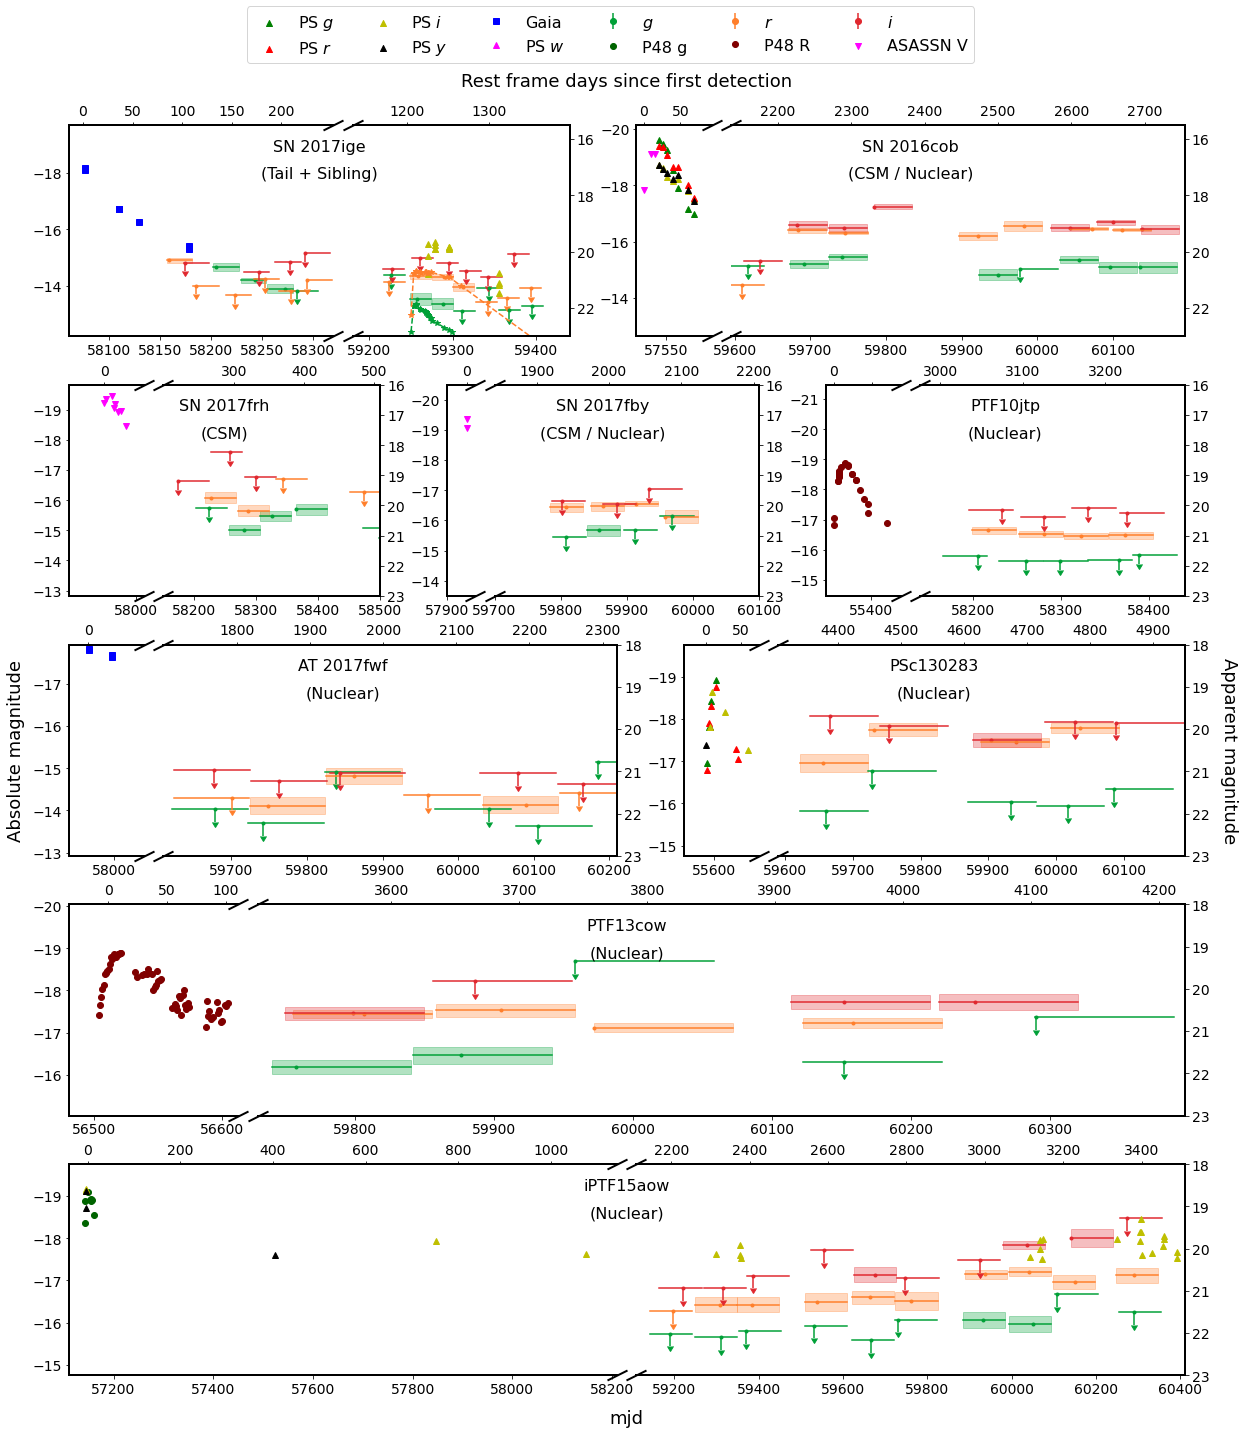
\includegraphics[width=0.95\textwidth]{../Images/chapter_4/weirdos.png}
    \caption{The nine objects whose late-time detections required a more rigorous investigation. Each object is shown in absolute and apparent magnitude (left and right axes respectively) and rest frame days since first detection and mjd (top and bottom axes respectively). I show the binned ZTF data with the late-time detections as well as pre-ZTF detections from other surveys (Pan-STARRS, Gaia, ASASSN, PTF) where available. For SN 2017ige a heavily extinct (E(B-V)$_\text{host}=1.2$ mag) light curve of SN 2020jfo is shown with dashed lines matching the late-time ZTF \ztfr-band detections. The objects are marked with the explanation for their late-time detections.}
    \label{weirdo_plots}
\end{figure*}


\textit{\textbf{SN 2017ige.}}
SN 2017ige was initially discovered and classified as a SN Ia in late 2017, only a few months before the start of ZTF. As it was relatively close by, the radioactive tail phase was identified in the ZTF binned data out to $\sim$200 d, before it faded below the noise limit. This tail matches well with the declining light curve seen in the early ($<$100 d) Gaia data (see Fig.~\ref{weirdo_plots}). \textsc{snap} shows that the SN is in the ZTF reference images, leaving a small ghost at its location in the difference images. 

At 1\,200 days after the SN tail faded below the noise limit, a small excess is detected in both the ZTF \ztfg~and \ztfr~bands that lasts around 90 days. In the difference images a small excess can be seen semi-overlapping the negative imprint left by SN 2017ige during this excess. Such a dipole signal would usually suggest imperfect image subtractions, but in this case it can also be interpreted as a separate transient slightly offset from the location of SN 2017ige being over-subtracted due to the presence of a SN in the reference images.

The late-time excess has been detected by Pan-STARRS in their \ztfi\ band, given the internal name PS21aos, and linked to SN 2017ige based on the sky position, confirming that the excess found in ZTF at late times is real. The Pan-STARRS \ztfi-band detections are brighter than what was found in the ZTF \ztfg- and \ztfr-bands, likely due to a combination of the ZTF detections being underestimated as a result of the ghost of SN 2017ige, as well as the late-time excess being intrinsically red ($g - r \approx 1$ mag). 

I use the duration and shape of the identified excess to test if it could be explained as a sibling transient. A light curve similar to that of SN 2020jfo \citep{Sollerman_2020jfo, IIp_ext}, a Type IIP SN with a relatively short plateau, fits the excess quite well in duration and absolute magnitude when a host extinction of $ E(B - V)$ = 1.2 mag is added. Given that the sky position at which the forced photometry was performed is only 0.99$\arcsec$ from the host nucleus of an edge-on galaxy, such a high amount of extinction is plausible. The original peak of the light curve of SN 2017ige in 2017 was not caught so a comparison with a similar extinction estimate cannot be made. Although close to the nucleus, inspection of the images shows that it is offset from the host centre as well as the original SN position. Therefore, I conclude that a Type II SN sibling with a relatively high value of extinction is an adequate explanation for this late-time excess.\\

\begin{figure*}
    \centering
    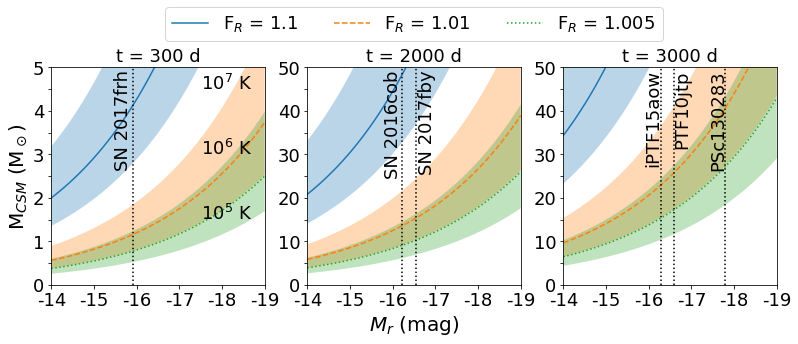
\includegraphics[width=16cm]{../Images/chapter_4/M_MCSM_rel.png}
    \caption{$M_\text{CSM}$ as a function of the \ztfr-band absolute magnitude $M$ for different assumptions of $t$ (panels), $T$ (shaded region), and $F_R$ (colours). The five objects for which I estimate $M_{CSM}$ in Sect.~\ref{weirdo_section} have been marked in the panel that has $t$ the closest to the detected signal. Decreasing shell thickness and temperature to mitigate $M_\text{CSM}$ is effective, though there is a limit to far this can be done while keeping realistic values for $F_R$.}
    \label{M_CMS_fig}
\end{figure*}


\textit{\textbf{SN 2016cob.}}
SN 2016cob was classified as a SN Ia of sub-class 91T-like at early times. There is light curve data from Pan-STARRS and ASASSN around peak and extending to just past 50 d from peak. In the ZTF binned data, this event jumps up from non-detections to detections in all three bands around $\sim$2200 d after first detection (Fig.~\ref{weirdo_plots}). The \ztfi-band data is included for completeness but does not have reliable baseline estimate ($>$30 points per region) so the values should be treated with caution. The detections are present in all bands at the same time and extend for at least 490 d at absolute magnitude of $-$15 to $-$17 mag. No SN-like transient can explain this long-lived flux excess.

Following the calculation in Section \ref{CSM_calc}, if I assume a CSM shell with a fractional radius of $\approx 1.005$ at a temperature of 10$^5$ K, this gives $M_\text{CSM}\approx$ 6 $M_\odot$. In Fig.~\ref{M_CMS_fig} I show the $M_\text{CSM}$ as a function of the \ztfr-band absolute magnitude, $M_r$, for three different times of the onset of the CSM interaction (300, 2000, 3000 d), three different $F_R$ values (1.1, 1.01, and 1.005) and temperatures of 10$^5$ to 10$^7$ K. This value of $M_\text{CSM}\approx$ 6 $M_\odot$ is a large CSM mass but around the same value as suggested to explain the interaction signatures seen in SN 2002ic \citep{Hamuy_02ic}. Based on this, I put SN 2016cob forward as a candidate late-time CSM interaction, though I note that it would require a very thin shell ($F_R$ = 1.005).

SN 2016cob is 0.7$\arcsec$ from the host nucleus, putting the nucleus on the same or an adjacent pixel in the ZTF observations. This leaves room for a host variability interpretation, though the host has no AGN according to its WISE colours. \textsc{snap} does not show any reduction or subtraction issues that could explain the ZTF detections as a spurious source either. 

The absolute magnitude, duration, and nuclear location are consistent with the ambiguous nuclear transient (ANT), ASASSN-20hx/AT 2020ohl \citep{Hinkle_Extreme_nuclear_transients/ANTs}. ANTs are events that cannot be easily classified into AGN activity or TDE. AT 2020ohl displayed a plateau or very slow decline in its optical light curves for $>$250 d relative to peak with an approximate plateau magnitude in the \ztfg\ztfr\ztfi\ bands of $-$17.5 mag. In Fig.~\ref{ANT_comp}, I compare the light curves of the shortlisted transients that are consistent with their host nuclei compared to AT 2020ohl. The flux excess at the position of SN 2016cob is shown as blue squares and is slightly fainter than AT 2020ohl. AT 2020ohl had an observed rise-time of 30 days \citep{Hinkle_Extreme_nuclear_transients/ANTs}, slightly larger than my smallest bins. This would explain why no rise is detected, as my time resolution is too poor to detect time variations of this scale. I can only observe a sudden appearance of a very flat light curve. Both late-time CSM interaction and an ANT are adequate explanations for the identified signal, and without additional information I cannot decisively point at one of these two explanations.\\


\textit{\textbf{SN 2017frh.}}
SN 2017frh was discovered by ASASSN and spectroscopically classified as a SN Ia. A flux excess was detected in the binned ZTF \ztfg- and \ztfr-bands at absolute magnitudes of $-$15.3 and $-$15.8, respectively. Only \ztfi-band upper limits were obtained. The detections were visible from the start of ZTF at a phase of 250 d after discovery and lasted for 190 d before disappearing behind the Sun. Nothing is detected after its return. The detections are found regardless of the baseline region that is used.

These detections are inconsistent with a normal SN Ia at these phases, which would have a significantly lower absolute magnitude ($M\approx-12$ mag) and also keep fading over time. If it were some type of sibling transient it would have to plateau at $-$15 to $-$16 mag for at least 180 d. No known class of SN shows this behaviour without the help of CSM interaction.

The late-time detections in SN 2017frh have a similar absolute magnitude and duration to the three late-time CSM interaction candidates that were presented in \citet{Terwel_2024_paper1}. However, the interaction in SN 2017frh starts significantly earlier ($\sim$240 d) than for those events. If I assume $F_R = 1.1$, a $M_\text{CSM}$ of 1.8 $M_\odot$ would be required to explain both the \ztfg\ and \ztfr\ bands assuming $T=10^5$~K. Raising the temperature to $T=10^7$~K gives $M_\text{CSM}\approx$ 4 $M_\odot$ for the \ztfg\ band and $M_\text{CSM}\approx$ 4.5 $M_\odot$ for the \ztfr\ band. SN 2017frh is shown in the left-hand panel of Fig.~\ref{M_CMS_fig}. If the $F_R$ is reduced to 1.01, then the the CSM mass is lowered to between 0.5 and 1.2 $M_\odot$. These mass estimates are in line with the suggestions of previous interacting SN events \citep{PTF11kx, Inserra_2016}. For these reasons, I classify SN 2017frh as a candidate SN with late-time CSM interaction.

The late-time excess at the position of SN 2017frh is also on top of the host nucleus, which could mean that the late-time signal is instead related to the host. However, the duration of the detected signal is the shortest of those shown in Fig.~\ref{ANT_comp}, although there is an observing gap at the end of the detected signal so no strict limit can be placed. Late-time CSM interaction signatures have been found in SNe Ia at similar phases \citep{2015cp}. Therefore, given the relatively low CSM mass required and the time frame of the interaction, I prefer the CSM interpretation for this late-time signal.\\

\begin{figure*}
    \centering
    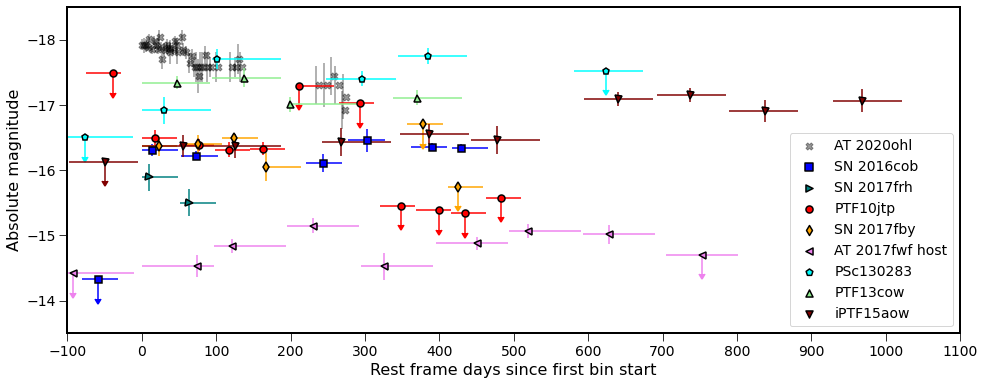
\includegraphics[width=\textwidth]{../Images/chapter_4/ANT_comp.png}
    \caption{Binned \textit{r}-band observations of the objects whose late-time detections are consistent with a galaxy nucleus (see Table \ref{weirdos}) and are potentially transient events unrelated to the original SN. Upper limits are shown with downward arrows. The \ztfr-band light curve of the slowly evolving ambiguous nuclear transient AT 2020ohl (ASASSN-20hx, \citealt{2020ohl_Hinkle}) is also shown for comparison. As the late-time signal in AT 2017fwf was found to be significantly offset from the SN location I show the processed light curve at the host nucleus location instead.}
    \label{ANT_comp}
\end{figure*}


\textit{\textbf{SN 2017fby.}}
SN 2017fby was discovered by ASASSN and spectroscopically classified as a SN Ia. The ZTF binned \ztfr-band detections at an absolute magnitude of $-$16.3 are found when the sky location returns from behind the Sun at 1940 d after discovery and lasts 200 d until it becomes unobservable again. The light curve stays roughly constant over this time frame. There are hints of a \ztfg-band excess as well but only one bin is above the $5\sigma$ threshold. After it comes back from behind the Sun nothing is detected anymore.

With a much stronger \ztfr-band signal compared to the \ztfg-band, one could argue for this being a reddened previously unknown sibling transient whose rise was missed due to it occurring while the sky position was too close to the Sun to be observed. However, the long plateau in the light curve of at least 190 d rules this out -- Type IIP SNe have plateaus that are generally significantly shorter than this \citep{IIL_IIP, SN_II_V_band_lcs}

If I assume the detections could come from a CSM shell with a fractional radius as low as $F_R \approx 1.005$, this gives a required CSM mass of $M_\text{CSM} \approx 5.5$ $M_\odot$ according to the calculation in Section \ref{CSM_calc}. This is around the upper end of the CSM masses that have been estimated for known SNe Ia-CSM such as SN 1997cy \citep{Chugai_2004}, SN 2002ic \citep{Chugai_2004, Inserra_2016}, and SN 2012ca \citep{Inserra_2016}. Therefore, I note SN 2017fby as a SN with potentially late-time interaction with a thin, massive shell of CSM.

Checking the difference images with \textsc{snap} shows a clear bright spot at the SN location during the period of detections and no clear issues before or after it, confirming the excess to be real. At a distance of 0.73" (0.66 kpc at the host redshift) from the host nucleus, a TDE or other nuclear transient would likely appear on the same or adjacent pixel in the ZTF images. Like for SN 2016cob, this makes it difficult to say whether late-time CSM interaction or an ANT is the best explanation for the signal (Fig.~\ref{ANT_comp}).\\


\textit{\textbf{PTF10jtp.}}
PTF10jtp was discovered by PTF and classified spectroscopically as a SN Ia. Detections were made in the ZTF binned \ztfr-band light curves starting at 3040 d after discovery. It had a $\sim 200$ day \ztfr-band plateau around $-$16.4 mag before the sky position became unobservable. When it came back from behind the Sun, there are $5\sigma$ upper limits that are about one magnitude deeper than the previous detections (not shown in Fig.~\ref{weirdo_plots}). 

The \ztfg-band has upper limits at approximately $-$15.5 mag during this entire period, while the \ztfi-band bins are not deep enough for a constraining upper limit to be placed. The baseline correction in \ztfr\ is significant and comparable between the later two baseline regions, but is somewhat smaller in the first region as it partially includes the period in which the excess was detected. This suggests that the excess was present in (some of) the reference images, and the late-time excess was present for longer than was found with the binning procedure. \textsc{snap} confirms this, as a slight excess can be seen in the difference images, followed by a small ghost at later times.

As this excess occurs over eight years after the SN, any SN Ia radioactive tail contribution at this magnitude can immediately be ruled out. Although there are only detections in one band, the limits placed on the colour together with the $>200$ day plateau limit the possibilities for a sibling, even with moderate values of extinction.

An unreasonably thin shell of CSM is needed to explain detections that are this late and still have an absolute magnitude of $M \approx -16.5$ while keeping the total mass of to be at most $M_\text{CSM} \approx 5$~$M_\odot$ in line with literature events. A CSM mass of at least 10 $M_\odot$ would be required. Therefore, I rule out CSM interaction as a likely explanation for this late-time flux excess. 

The sky location is 1.11$\arcsec$ from the host nucleus, and \textsc{snap} also shows that the excess is slightly offset from the SN location in most frames and consistent with the host nucleus. The long duration of the excess, combined with the central location, suggests host activity is the cause, although it is not an AGN according to its WISE colours. Therefore, a nuclear transient is the most likely explanation for these late-time detections. Its light curve is shown compared to the ANT AT 2020ohl in Fig.~\ref{ANT_comp}, where it is seen to be plausibly consistent in duration and absolute magnitude.\\


\textit{\textbf{AT 2017fwf.}}
This object was only detected by Gaia at early times with no spectrum obtained, preventing even a speculative classification based on the photometry. It is detected in ZTF binned \ztfr-band data starting at 1810 d after discovery and this lasts for 420 d. The light curve rises from $-$14 to nearly $-14.7$ mag before slowly fading again. Despite having upper limits around the same magnitude as \ztfr, nothing was detected in \ztfg. The \ztfi-band limits are shallower and less constraining. \textsc{snap} shows that the excess is real, but located at the nucleus location 1.67$\arcsec$ from the SN. Therefore, CSM interaction can be ruled out. The long timescale of the transient also makes a SN-like transient unlikely. 

Performing forced photometry at the host nucleus location reveals its properties much more clearly, being visible for nearly 700 days and reaches $-15.2$ mag at its brightest (see Fig.~\ref{ANT_comp}). This is longer by nearly 300 days and brighter by nearly 0.5 mag than the values given in Table \ref{weirdos} for the forced photometry at the SN position. The host galaxy is not an AGN according to its \textsc{wise} colours. The excess is still very faint for a TDE unless it is heavily reddened, although a reddened TDE would likely have been bright enough in the \ztfi-band to still be visible. However, an ANT could be possible, though the signal is three mag fainter than AT 2020ohl but also visible for over twice as long. Faint nuclear variability could also be possible and there is some scatter in the light curve but with my 100 d bins for the light curve, small-scale variability can not be identified. Therefore, I can only conclude that some sort of nuclear variability is present. 

I note that a sibling transient is also detected by ZTF in this host galaxy (SN 2020ackb, SN IIP), though it is at a distance of 5.23$\arcsec$ and has no effect on the forced photometry at the location of AT 2017fwf. The time at which the sibling was visible also does not correspond with the detected host variability.\\


\textit{\textbf{PSc130283.}}
PSc130283 was detected by Pan-STARRS and spectroscopically classified as a SN Ia. At 4340 d past discovery, ZTF-detections are found in the \ztfr-band at an absolute magnitude of $-$17 mag before brightening again to $-$17.8 mag in the next bin and staying there with variation $\leq 0.5$ mag for the remainder of the light curve (at least 520 d). The non-detections before the start of the excess were up to 1.5 mag lower, suggesting that the excess started suddenly rather than a gradual brightening. During the entire late-time excess, the \ztfg-band stays with $5\sigma$ upper limits at $-$16 mag.

Detections this late ($\gtrsim 4300$ days) and bright ($M \sim -18$ mag) cannot give a reasonable $M_\text{CSM}$ in Eq.~\ref{CSM_calc} unless a temperature around $10^{4.5}$~K and $F_R < 1.0005$ is assumed giving an unreasonably thin shell and no extinction between the SN site and us. Therefore, I rule out CSM interaction as a likely cause of the late-time flux excess.

\textsc{snap} shows a clear excess that is consistent with the SN location, and no ghost or residuals before the excess starts or image defects that could explain these detections. However, the flux excess is only 0.44$\arcsec$ from the host nucleus, although the host is not an AGN according to its WISE colours. The host has a history of small variability that causes sparse detections (including a detection that put its discovery date over 400 days before the SN explosion), which points to the ZTF detections in the binned data to be host related. Out of all excesses plotted in Fig.~\ref{ANT_comp}, PSc130283 is the brightest. It is very similar in brightness to AT 2020ohl though a bit longer in duration. These properties, combined with its relatively sharp rise suggest nuclear variability, such as an ANT, could explain these detections.\\


\textit{\textbf{PTF13cow.}}
PTF13cow was discovered by PTF and classified as a SN Ia. The late-time detections in the ZTF \ztfg\ztfr\ztfi\ bands begin 3510 d after discovery at absolute magnitudes of $-$16.0 and $-$17.3 mag in the \ztfg- and \ztfr-bands, respectively. There are detections in the \ztfi-band, however the baseline is too small for these to be considered any further here. The \ztfr-band detections last for at least 610 d. The \ztfg-band is only detected at the start but is significantly fainter and disappears below the detection threshold earlier. This long timescale rules out SN-like transients as a cause for the excess.

\textsc{snap} shows there is a clear excess in the images, and despite the host nucleus distance being only 0.56$\arcsec$ from the SN location, the SN location and host nucleus are on different pixels. The excess has a preference to be at the host nucleus location, suggesting it is the cause of the signal. However, the host nucleus is not an AGN according to its WISE colours. The duration of over 560 d and a peak absolute \ztfr\ band magnitude of $-17.4$ of the identified late-time excess is similar to AT 2020ohl, meaning that an ANT could explain these detections.\\


\textit{\textbf{iPTF15aow.}}
iPTF15aow was discovered by the intermediate PTF survey (iPTF), as well as detected in Pan-STARRS and classified as a SN Ia. The late-time detections begin in the \ztfr-band at 2280 d after discovery at $-$16.4 mag. There are only upper limits in the \ztfg- and \ztfi-bands at this time, but at later times some detections in these bands are made. The detections last for at least 1050 d and slightly brighten with time to $-$17.2 mag in the last bins. The long-lived nature rules out SN-like transients at the same position as the original SN Ia. 

Even when assuming a scenario where the \ztfr-band interaction stays at the level it was discovered at for the entire duration it was detected, $> 5$ M$_\odot$ of CSM is required in a very thin, low temperature shell. However, the signal increases in strength over time, which would increase the required CSM mass. On top of that, no known SN Ia with CSM interaction has interaction as long as the late-time excess is found for or with the strength increasing over time, further disfavouring the CSM explanation.

The host nucleus is close by at 0.92$\arcsec$ but from \textsc{snap} the transient does not look to significantly favour the SN or host nucleus location over the other. The host is not an AGN according to its WISE colours (W1 -- W2 = 0.077 mag, W2 -- W3 = 1.564 mag). 

Pan-STARRS has some detections in the unforced photometry at the SN location, the first being at the time of iPTF15aow's discovery. However, it has no internal name. In the years after the first detection there are a some detections in their \ztfi-band but these are likely spurious because of a significant number of upper limits in between them that are not shown in Fig.~\ref{weirdo_plots}. The number of Pan-STARRS \ztfi-band detections increased significantly after $\sim$2900 d after discovery, which corresponds to the brightest part of the binned ZTF detections.

The duration, shape, and close proximity to the host nucleus of the excess point to it being most likely host related. It has a similar brightness to AT 2020ohl, but has a several times longer duration and is still going. The fact that it continues to brighten is also very unusual. None of these signatures are consistent with what would be expected from a late-time CSM interaction.


\section{Discussion}
\label{Pre-ZTF_discussion}
In this study I gathered a sample of 8707 transients that were first detected between 1 January 2008 and 31 December 2017 whose locations have been observed by ZTF between 2018 and 2023. By performing forced photometry on all ZTF observations at the target locations I created late-time light curves for all transients in my sample, often reaching over 10 years after the first detection. Using the pipeline from \citet{Terwel_2024_paper1} I binned the ZTF light curves to search for the presence of faint previously undetected signals. I find 98 cases with detections that cannot be explained as false positives due to observational, reduction or software issues. These objects can be split into four groups: i) ongoing signatures of bright and/or nearby transients that were still detectable at the start of ZTF, ii) sibling transients at nearly the exact same location on the sky, iii) known variable sources such as AGN and variable stars, and iv) nine late-time flux excesses that required a more in-depth examination. Of these nine, I concluded that one was a sibling SN, five cases were nuclear transients close to the SN locations, two objects where it is unclear whether the ZTF signal is host or CSM related, and one SN whose ZTF-detections are most consistent with late-time CSM interaction.


\subsection{Rarity of late-time signals from SNe}
I started my search for late-time signals based on the positions of 8\,707 transients discovered before ZTF. Table~\ref{recovered_obj_breakdown} shows the number of objects that had detections in ZTF, split over the six main types of SNe I distinguish between in my sample. In the sections below, I discuss the main conclusions for each of the likely classes (siblings, nuclear, CSM) of the late-time signals detected.

\begin{table}[]
   \caption{Number of recovered signals for each SN type in my sample. As it is unclear whether SN 2016cob and SN2017fby should be counted as nuclear transients or due to CSM interaction, they have been counted in both.}
    \centering
    \begin{tabular}{cccccccc}
        \hline
        \hline
        Type & No.  & \multicolumn{2}{c}{Siblings}  & \multicolumn{2}{c}{Nuclear} &  \multicolumn{2}{c}{CSM}  \\
        && No. & \% & No. & \%& No. & \% \\
        \hline
        Ia & 5618 & 6 $^{(a)}$ & 0.1 & 7 & 0.1 & 3 & 0.1\\
        II & 1494 & 4 $^{(b)}$ & 0.3 &  0 & 0 & 0 & 0 \\
        Ib/c & 385 & 0 & 0 & 0 & 0 & 0 & 0 \\
        IIn & 310 & 0 & 0 & 0 & 0 & 0 & 0 \\
        I & 69 & 0 & 0 & 0 & 0 & 0 & 0 \\
       Ibn & 18 & 0 & 0 & 0 & 0 & 0 & 0 \\
        \hline
    \end{tabular}
     \label{recovered_obj_breakdown}
    \begin{flushleft}
        $^{(a)}$ This includes the unconfirmed but likely sibling at the position of SN 2017ige determined from my binned light curve analysis.  \\
        $^{(b)}$ This includes one sibling pair (SN 2009hz/AT 2018iml) where the ZTF transient was a likely CV based on its light curve. \\
    \end{flushleft}
\end{table}


\subsubsection{Siblings}
Within the uncertainties the rate of siblings found is the same for the different groups of objects with the SN Ia and Type II SN classes having rates of sibling discovery of 0.1 -- 0.2 \%. The percentage is similar, given the large uncertainties associated with low numbers of events, to the percentage of siblings found in \citet{Terwel_2024_paper1} over a smaller time frame. These rates can be taken as lower limits because of observing gaps, which would result in transients being missed. In total, I found 10 siblings out of 7718 light curves that could be binned gives a lower limit on the rate of siblings of $0.13\pm0.04\%$. SN Ia sibling pairs along the same line of sight may be useful for constraining the origin of reddening in SN Ia light curve fitting for cosmology \citep{DR2_siblings}, but a larger sample would be required for meaningful constraints. 


\subsubsection{Serendipitous nuclear transient detections}
\label{sec:discussion:nuclear}
I identify five late-time signals that were most likely due to host activity that was (partially) picked up in the forced photometry at the SN location. This was determined due to a combination of the shape and duration of the late-time light curve, as well as the inferred $M_\text{CSM}$ from the absolute magnitude and delay between the main SN and late-time detections being unrealistically high in the best case scenario. I also identify signals at the positions of two events (SN 2016cob and SN 2017fby), where the inferred cause could be CSM or nuclear activity, bringing the total to seven potential nuclear events (see Table \ref{recovered_obj_breakdown}).

In Fig.~\ref{ANT_comp}, I show the late-time excess light curves for which nuclear transients can not be ruled, along with the late-time light curve of SN 2017frh for completeness, although I prefer a CSM interpretation for it. The light curves are shown as absolute magnitude in the \ztfr-band against the time since the first binned data where a flux excess is identified. I also show the ANT AT 2020ohl \citep{2020ohl_Hinkle} for comparison. AT 2020ohl is slightly brighter than most of these transient events apart from PSc130283. My events are also longer lasting, ranging from $\sim$200 days up to $\sim$1100 days. This could mean that there is a previously unknown population of lower luminosity ANTs that require deeper (binned) observations to be detected.

\citet{wiseman_ztfants} showed that their sample of ANTs all have changes in their WISE \textit{W1}- and \textit{W2}-band observations, with a slight delay compared to the optical. The WISE light curve for my potential nuclear transients were investigated, but unfortunately these light curves use the total measured flux from the source. As the hosts of my nuclear transients have an apparent magnitude of around 15 mag in these bands and the optical variability I have identified is $\geq5$ mag fainter than that, any MIR variability is likely to be heavily suppressed into the noise of the WISE light curves.

CL-AGN show variability on similar timescales as those I have found here \citep{CLAGN}. However, CL-AGN are a subset of AGN and the galaxies hosting my transients are not AGN according to the WISE criterion from \citet{WISE_crit}. My objects are also much lower luminosity that seen for CL-AGN, which also makes this classification unlikely.


\subsubsection{CSM interaction}
In \citet{Terwel_2024_paper1}, I estimated an intrinsic rate, through simulations of the detection efficiency for three out of 3\,628 SNe Ia with potential late-time CSM signals, of $<$0.5 per cent of normal SNe Ia displaying late-time ($>$ 100 d post peak) CSM signatures. \cite{GALEX_Late_CSM} estimated a rate of late-time interaction in $<$5 \% of SNe Ia. In this work, I identified three SNe Ia whose signals in ZTF cannot be ruled out as being due to late-time CSM interaction, giving a raw rate of late onset CSM interaction of $\leq$0.1 \% for the 5\,618 SNe Ia in this sample (see Table \ref{recovered_obj_breakdown}). No potential late-time signature from CSM interaction was identified in any other SN type.

SN 2017frh is my best candidate for late-onset CSM interaction. It has the earliest period of late-time detections ($\sim 300$ days after the first detection), and a similar estimate for $M_\text{CSM}$ as \citet{2015cp} found for SN 2015cp. If I assume a nova-like shell at $T=10^7$~K, I get a reasonable CSM mass of $M_\text{CSM} \approx 4$ $M_\odot$ (although see the discussion of the limitations of my CSM estimates in Section \ref{sec:discussion:limitations}). My two other CSM candidates, SN 2017fby and SN 2016cob, have late-time signals five years after the SN was first detected. When I assume these objects to have shells of similar thickness as the shell in SN 2017frh, a CSM mass estimate of $\sim 5$ $M_\odot$ can be found for these objects as well. These estimates are lower limits, as no host extinction is assumed for objects in regions of galaxies where significant amounts of extinction can be expected.

I have not performed detailed rates calculations for the events discovered in this study. However, there are $\sim600$ objects in my sample that were first detected less than 300 days before the start of ZTF, and I have one candidate with a late-time signal detected around 300 days after discovery. This gives a raw rate of 0.2 \% when not taking into account any bias. Two additional candidates have their detections in the fifth year after the explosion. About half of my sample exploded less than five years before the start of ZTF, and have their fifth year observed the survey. Two of these are candidates for having late-time CSM interaction at these phases, giving a rate of 0.05\% when not taking any bias into account. My rough estimates of the rates suggest similar values to those of \citet{Terwel_2024_paper1}, within the uncertainty of the small numbers of events detected.

The three events in \citet{Terwel_2024_paper1} that were identified as consistent with CSM interaction, were also close to their host nuclei. As discussed in \citet{Terwel_2024_paper1}, this could suggest a preference for CSM interaction to occur in SNe Ia in these environments or an alternative explanation is that they are caused by nuclear activity. However, as discussed in Section \ref{sec:discussion:nuclear} and shown in Fig.~\ref{ANT_comp}, these late-time signals are similar but not entirely consistent with nuclear activity/transients.


\subsection{Limitations}
\label{sec:discussion:limitations}
I found a large group of SNe whose tail was detected by ZTF but never properly picked up by the survey -- all of them required more thorough baseline corrections as the transient was present in the reference images. Several of these were exceptionally long lived, with detections in the binned data being recovered over a year after the start of ZTF. I also found some periodic variable sources that have this behaviour for at least the length of the survey, making it impossible to generate proper reference images or apply a good baseline correction. Both groups can leave behind a ghost, which is an imprint at the transient location when the object is fainter than it was in the references. These events can be recovered from the data, particularly if different time frames for estimating the baseline correction are used, but they are often hidden if a baseline correction is not applied. 

As in \citet{Terwel_2024_paper1}, the magnitude limit of the binning technique is set by the magnitude limit of the references, as their uncertainty starts to dominate when more epochs of observation are binned together. One way to improve the sensitivity, though computationally expensive, is to find a region where I am certain there is no excess at the SN location and use it to generate custom references to use for difference imaging. This would immediately lessen the need for a baseline correction significantly, as an adequately chosen reference region already has this built in automatically.

Any search for late-time signals from SNe will also be dependent on the constraints placed on the sample. I required a first detection between 2008 and 2018 and a classification or candidate SN status. My sample contained several false positives from objects that had spurious detections within the initial sample definition, but a SN (which was classified) exploded years later and was observed by ZTF. Siblings, whether they are true SN siblings or false due to spurious detections or projection effects, can be confused if they occur at (nearly) the same position in the sky. One way to remove false siblings, like AT 2017keg and SN 2013ld, is to require a spectroscopic classification in the same time period as the first detection, though this would also remove objects like AT 2017gcd as in that case only the second sibling was classified, and candidate objects like AT 2017fwf and AT 2017gpv that were never spectroscopically classified at all.

I attempted to estimate the CSM mass required to produce late-time detections as bright as I observed them, assuming Bremsstrahlung to be the main mechanism producing light. In most cases when assuming a thin nova-like shell the required CSM mass is above $\sim 10$ $M_\odot$, with the only exception being SN 2017frh due to its relatively short delay time between the SN explosion and late-time detection. For SN 2016cob and SN 2017fby the only way to get realistic CSM mass estimates is by assuming a colder CSM and a lower $F_R$, which could be explained by the shell size that is needed for interaction to start over five years after the SN (see the end of Sect.~\ref{CSM_calc}). \citet{2015cp} argue that the simplified assumption of Bremsstrahlung being the main mechanism is largely responsible for the high CSM mass estimates. They find an upper limit of $M_\text{CSM} \sim 7$ $M_\odot$ for SN 2015cp with this method, while \citet{2015cp_radio} find $M_\text{CSM} \lesssim 0.5$ $M_\odot$ using radio non-detections. They argue that line emission from elements such as \ion{H}, \ion{Mg}, and \ion{Ca}~are instead the main contributors to the emission. However, as line emission requires much more assumptions on the state of the emitting gas, it is much more complicated to derive a good estimation for $M_\text{CSM}$ for it. 

Even if I assume that Eq.~\ref{M_CSM_eq} gives an upper limit and the better estimates from modelling of radio observations to be $\sim$14 times smaller (based on the two estimates for SN 2015cp), the CSM interaction scenario for late-time signatures at 2000 -- 4000 days post initial SN discovery is still unlikely for five of my events that are also potentially due to nuclear activity. I have also not considered the impact of extinction in the host galaxy, which is likely non-negligible given the nuclear location of the transients considered. The CSM mass can be reduced by assuming a smaller $F_R$, but the effect is limited unless I consider shells that are unphysically thin. However, thin shells are not ruled out by a several hundred day long period of late-time detections, as the time delay due to the large radius of the shell can smear even a 1~s interaction signal out over several months. This shows that it is very difficult to properly constrain the CSM mass from photometry alone without knowing the mechanism powering it and more detailed theoretical studies.

\section{Conclusions}
\label{Pre-ZTF_conclusions}
In this work I have presented a search for late-time signals observed in ZTF from transients that were first detected up to ten years before the start of the survey. By binning the ZTF data I was able to go nearly one magnitude below the noise limit of unbinned data points. My sample consists of 8\,707 unique objects that are in the ZTF footprint and could be searched for late-time signatures. By careful inspection of the ZTF images and comparison to known classes of transients, I determined the most likely source of the late-time signatures I identified at the positions of 98 transients discovered prior to ZTF starting. My main conclusions are:

\begin{enumerate}
    
    \item I identified several very long-lived transients that began pre-ZTF and continued for many hundreds to thousands of days. These include the SLSN IIn, SN 2015da, with data extending to eight years after discovery and the spectroscopically unclassified AT 2017gpv, whose bumpy long-lived light curve (detected up to nearly four years post discovery) is reminiscent of iPTF14hls \citep{iPTF14hls_Iair,Sollerman_2019_iptf14hls} and SN 2020faa \citep{Yang_2021_20faa, 2020faa_hidden_shocks}. 
    \item I found 10 confirmed pairs of sibling transients where the pre-ZTF and ZTF siblings are at nearly the same sky position. One additional unconfirmed but likely sibling transient was identified when applying my binning technique at the positions of SN 2017ige (it was detected by Pan-STARRS with internal name PS21aos). In the majority of the cases, one of the siblings was never spectroscopically classified. I also found two pairs where the ZTF transient was mistakenly reported as a pre-ZTF transient due to spurious detections from the nearby host.
    \item I found six flux excesses at the position of events classified pre-ZTF as Type II SNe (three Type II, one IIn and two SLSN-II) consistent with AGN activity in known AGN host galaxies. I speculate that some of these were likely misclassified at the time of the pre-ZTF detection.
    \item I found five flux excesses that were consistent with activity of the host nucleus close to the location of the original transient. The brightness, light curve shape, and duration are broadly consistent with (ambiguous) nuclear transients, showing that there may be a previously unknown population of faint nuclear transients that requires deeper (binned) observations to be discovered.
    \item I found three flux excesses that were consistent with late-time interaction with a $4 - 5\ M_\odot$ CSM shell, assuming Bremsstrahlung as the main emission mechanism. In two of these the signal is $\sim5$ years after the SN and could also be explained by a nuclear unrelated to the SN. SN 2017frh is my best candidate with a signal $\sim300$ days after the SN consistent with a $4\ M_\odot$ nova-like CSM shell at $10^7$ K. Although a nuclear transient can not be completely ruled out.
 \end{enumerate}

The Vera C. Rubin Observatory's Legacy Survey of Space and Time \cite[LSST;][]{LSST} will observe the transient universe several magnitudes deeper than ZTF. This is crucial for finding faint interaction signals like those I have searched for in this chapter, as I have shown these to be rare. Increasing the volume that can be probed is the best way to find new events and follow them up. Current samples of objects will be observed at late times by LSST, making it possible to do a late-time signal search in real-time. By using a well-defined and complete sample such as the ZTF SN Ia DR2 \citep[][, Smith et al.~in prep.]{DR2_Overview}, Bright Transient Survey \cite[BTS;][]{BTS_I, BTS_II}, or a similar sample for ZTF SNe first detected in 2021+ as the basis for a similar search of late-time signals observed with LSST, it will also be possible to properly estimate their rates. Not only can these methods be used to search for late-time CSM interaction, but as I have shown they are also suitable for finding other weak signals, such as faint nuclear transients.


\end{document}
%!TEX root = ../main.tex
\documentclass[a4paper,oneside,12pt, class=Latex/Classes/PhDthesisPSnPDF, crop=false]{standalone}
\usepackage{setspace}
\begin{document}
\doublespacing
\chapter{A real-time search for Type Ia SNe with late-time CSM interaction in ZTF}
\label{chap:Real-time}
In chapters \ref{chap:DR2_search} and \ref{chap:pre-ZTF_search} I searched for late-time signals in old transients, with most results being found after the period of activity. Follow-up was only attempted for SN 2019ldf (photometric) and SN 2020alm (spectroscopic) in section \ref{Additional_tests}, but these provided no further signs of late-time CSM interaction. In order to understand more about the late-time signals that are recovered by binning the ZTF light curves, it is crucial to follow promising objects up using larger telescopes.

For this reason, I automate my pipeline to search a sample of SNe Ia observed by ZTF for currently active late-time signals using the latest observations. By doing this regularly, it is possible to find promising objects early and follow them up. My position as a student support astronomer at the Isaac Newton Group of Telescopes (ING) and Nordic Optical Telescope (NOT) proved to be extremely advantageous in obtaining time to observe targets using a 2.5 m telescope, but this time has very low priority. It proved to be crucial for quick follow-up of several objects that are presented in this chapter, especially SN 2020qxz (see section \ref{sec:SN2020qxz}).

This chapter is based on Terwel et al., (in prep.), which is currently being written and will be submitted to A\&A. The sample selection, data reduction, analysis and interpretation were performed by me. Where relevant, I have noted the specific parts that were carried out by collaborators. In section \ref{data} I present the sample used in the real-time search and explain where the latest observations come from. Section \ref{analysis} describes the automated pipeline, details the telescopes used in the follow-up campaign, and gives a short overview of the reduction. In section \ref{results} I describe the results for the promising objects that were found during the run of the real-time search. These are discussed in section \ref{discussion}, and I conclude in section \ref{conclusion}.


\section{Data}
\label{data}
To create a SN Ia sample to search for late-time CSM interaction in real time, I collect all spectroscopically classified SNe Ia in ZTF using the Fritz broker \citep{skyportal2019, Skyportal} and selected those objects that were first detected before 8 July 2023 (mjd 60133). Using this date cutoff ensures that all targets are over 100 days old at the start of the real-time search, and any new observations can be considered to be late-time observations of the SNe. This gives me a sample of 6\,914 SNe Ia. Using the \textsc{fpbot} package \citep{fpbot}\,\footnote{\url{https://github.com/simeonreusch/fpbot}} I construct the most up-to-date ZTF light curves for every object in my sample. ZTF uses difference imaging to remove constant sources from the science images and isolate the transient. Then, \textsc{fpbot} forces a PSF fit at a given location in the difference images to construct a light curve at that position spanning the entire survey.

As this sample contains all ZTF SNe Ia up until the first half of 2023, this naturally includes the entire ZTF SN Ia DR2 \citep[][Smith et al., in prep.]{DR2_Overview}, which have previously been examined for late-time signals in \citet{Terwel_2024_paper1}. 69 objects that were not available on Fritz when I made my sample have been excluded. However, as the latest data point used in \citet{Terwel_2024_paper1} is on 26 June 2022 (mjd 59756) I probe their SNe at later phases, and they could (have) become active after the time period examined by \citet{Terwel_2024_paper1}. Therefore, checking the same sample again could identify new late-time detections.

I aim to find late-time excesses while they are active, so the light curves have to be regularly updated with the latest observations. The ZTF survey is split into three parts: 40\% is a private partnership survey whose data I can access immediately after the observation and becomes publicly available after 18 months. 40\% is a public survey whose data is released every three months after a three-month proprietary, resulting in a three to six-month delay. The last 20\% is private Caltech time, whose data is released publicly after 18 months.

I use the binning method from \citet{Terwel_2024_paper1} to search for faint signals, binning observations over 100 days after the SN peak together in bins of 25, 50, 75, and 100 days. (see section~\ref{analysis}). The light curves do not have to be updated daily, as it will take several observations to push the detection limit deep enough to detect a faint signal in the latest bin. As the smallest bin size in the pipeline is 25 days, I aim to be able to create one additional bin each time an object is updated. I therefore split the sample into 28 lists and update the objects in one of these each day. This results in every object in the sample being checked and updated once every four weeks.

\section{Analysis}
\label{analysis}
Each time the light curves of the SNe Ia in my sample are queried and updated, they are run through the analysis pipeline from \citet{Terwel_2024_paper1}. This pipeline takes all observations at a given sky position and after pre-processing (including applying a baseline correction to correct for systematic offsets across the light curve, see e.g. \citealt{Yao_baseline_corr, Miller_baseline_corr}) and finding the SN peak, it will bin all observations in each band that are over 100 days after the SN peak in bins that have a size of 25, 50, 75, or 100 days. By doing so, the noise in the data is reduced, allowing to probe objects that are up to nearly a magnitude below the noise limit of single observations (m $\approx20.5$ mag) at the price of a reduction in the time sensitivity. This method is able to push the detection limit until the magnitude limit of the used reference images become the dominant source of uncertainty, which is around $\overline{\text{m}} \approx21.8$ mag for ZTF \citep{ref_uncert}.

When the pipeline detects a possible late-time signal, whether currently or previously active, the object is rechecked manually to determine the possible origin of the late-time time signal and if it should be followed up. Possible explanations for the signal include, e.g., false positives due to a baseline offset, contamination from a possibly active host nucleus, known transients that are detectable over 100 days after the SN peak, or sibling transients at nearly the same sky position (see sections \ref{DR2_results} and \ref{Pre-ZTF_results} for more details on these groups of objects). If the late-time signal is deemed real but has clearly faded again before it was found, all I can do is an analysis akin to that of chapters \ref{chap:DR2_search} and \ref{chap:pre-ZTF_search}. However, if the signal is still active, I attempt to follow it up as quickly as possible using bigger telescopes to gain deep photometry (to confirm the late-time signal in a single observation) and spectroscopy (to search for spectral signature of the signal found in the binned ZTF observations. After all pre-existing light curves were generated, the real-time monitoring program started on 13 November 2023 (mjd 60261) and ran until 9 July 2024 (mjd 60500).


\subsection{Follow-up observations and reduction}
\label{sec:reduction}
Follow-up observations of promising late-time detections were carried out with the Nordic Optical Telescope (NOT) and the Gran Telescopio CANARIAS (GTC) at Observatorio Roque de Los Muchachos, La Palma. I obtained the NOT data through staff time, except for the SN 2020qxz host spectra which I obtained through fast-track proposal p69-401 of which I am the PI. The GTC data was obtained and reduced by Dr. Lluís Galbany. General information on these telescopes is given in sections \ref{NOT} and \ref{GTC}, respectively. An overview of the reduction process is given in section \ref{reduction}. The NOT photometry is reduced using a custom pipeline in \textsc{python} using the \textsc{astropy} package. The GTC photometry is reduced with \textsc{iraf}. After the basic photometry reduction, difference imaging is done using \textsc{autophot} \cite{Autophot}\,\footnote{\url{https://github.com/Astro-Sean/autophot}} by Dr. Seán Brennan, using observations from Pan-STARRS \citep{Pan-STARRS1} or the Sloan Digital Sky Survey \citep[SDSS, ][]{SDSS-I-II, SDSS_DR4, SDSS_telescope} as reference images.

GTC+OSIRIS+ spectra were obtained at the location of SN 2019zbq at late times using the R1000R and a 1.0$\arcsec$\ slit. They were reduced using a custom pipeline based on \textsc{pypeit} \citep{pypeit:joss_pub, pypeit:zenodo}.

The NOT+ALFOSC spectra obtained at the position of SN 2020qxz were obtained with grism 4 with a 1.3$\arcsec$\ slit on the 20, 30, and 31 March 2024 and 13, 14, and 15 April 2024. Spectra of the host galaxy of SN 2020qxz were obtained with the NOT+ALFOSC on 3 May and 19 June 2024 using a 1.0$\arcsec$\ slit. For these spectra I used the WG345 order-blocking filter to remove second-order contamination of blue light in the red part of the spectrum. This was not used in the spectra of the transient itself as it was already very faint, and removing an extra $\sim$10\% of the light that hits the detector would decrease the SNR of the spectra. These spectra were reduced using a pipeline made by Dr. Steve Schulze based on \textsc{pypeit}\,\footnote{\url{https://gitlab.com/steveschulze/pypeit_alfosc_env}}, taking care to separately extract the different sources lying close together.

Since a signal due to CSM interaction is not expected to evolve on the timescale of a few days \citep[e.g.,][]{2015cp}, I combined the spectra obtained in March 2024 to gain a combined exposure time of 3 hours on the target. I also combined the spectra taken in April 2024 together to obtain a second spectrum with 2 hours and 40 minutes on the target. These will be called the `March' and `April' spectra of SN 2020qxz below (see section \ref{sec:SN2020qxz}).


\section{Results}
\label{results}
\begin{sidewaystable*}
    \centering
    \caption{Objects with a detected late-time signal in the binned ZTF light curves. The first two columns give the ZTF and IAU names of the object, followed by the position, classified type, and redshift. The classifications are taken from the ZTF DR2 release \citep{DR2_spec_div, DR2_diversity}, except for SN 2022uej, whose classification comes from TNS. Column 7 gives the peak date of the SN, and column 8 gives the discovery date of the late-time signal. Column 9 gives the start of the first bin that is part of the late-time signal with the bin size that best shows the signal. Column 10 gives the duration of the late-time signal in rest frame days. The last column is a comment on the nature of the late-time signal. The table is divided into two parts, with the objects that were not followed up above and objects that were followed up below the division line.}
    \resizebox{\textwidth}{!}{
    \begin{tabular}{ccccccccccc}
        \hline
        \hline
        ZTF name & IAU name & RA & Dec & Type & $z$ & MJD$_\text{peak-SN}$ & MJD$_\text{disc-lt}$ & MJD$_\text{start-lt}$ & $\Delta t$ (day) & Comment\\
        \hline
        ZTF18abtqevs & SN 2018grt & 00:04:36.30 & 51:59:37.63 & Ia-norm & $0.042\pm0.003$ & 58372 & 60279 & 59712 & 162 & \color{red} \citet{Terwel_2024_paper1} \color{black}\\
        ZTF19ablekwo & SN 2019mse & 00:15:21.36 & 46:44:08.64 & Ia-norm & $0.088\pm0.004$ & 58715 & 60283 & 59167 & 1170 $^{(2)}$ & \color{red} \citet{Terwel_2024_paper1} \color{black}\\
        ZTF20abjfufv & SN 2020tfc & 22:17:00.81 & 30:39:20.97 & Ia-norm & $0.031\pm0.001$ & 59116 & 60269 & 59671 & 804 $^{(3)}$ & \color{red} \citet{Terwel_2024_paper1} \color{black}\\
        ZTF20aaifyfx & SN 2020alm & 16:52:01.49 & 23:32:22.77 & Ia-norm & $0.06001\pm0.00001$ & 58873 & 60271 & 59624 & 826 $^{(3)}$ & \color{red} \citet{Terwel_2024_paper1} \color{black}\\
        ZTF22abgbbez & SN 2022uej & 07:19:57.72 & 46:00:59.00 & Ia & $0.03272\pm0.00008$ & 59839 & 60454 & 60168 & 212 & \ztfr\ detected only\\
        ZTF19acgonwy & SN 2019spg & 08:21:48.09 & -14:04:12.00 & Ia & $0.073\pm0.001$ & 58790 & 60353 & 58891 & 110 & Nuclear\\
        ZTF19abvvpoh & SN 2019pqn & 16:04:03.86 & 18:28:18.46 & Ia-norm & $0.03720\pm0.00001$ & 58745 & 60458 & 60436 & 62 $^{(3)}$ & Nuclear\\
        \hline
        ZTF20acpbbqf & SN 2020yvs & 10:24:22.78 & 41:42:25.97 & Ia-norm & $0.04453\pm0.00001$ & 59160 & 60268 & 59260 & 1127 & False positive\\
        ZTF20aazhzna & SN 2020jsa & 14:24:23.94 & 26:41:23.00 & Ia-norm & $0.03657\pm0.00001$ & 58992 & 60431 & 60315 & 72 & Nuclear\\
        ZTF18acaucsw & SN 2021nbt & 22:42:29.54 & 01:49:53.84 & Ia & $0.07\pm0.01$ & 59359 & 60283 & 59718 & 730 $^{(3)}$ & Nuclear / ANT\\
        ZTF19adcdgca & SN 2019zbq & 09:08:53.91 & 55:19:08.86 & Ia & $0.04678\pm0.00001$ & 58859 & 60261 & 59958 & 518 $^{(3)}$ & Nuclear / ANT \\
        ZTF20abqkbfx & SN 2020qxz & 18:04:00.24 & 74:00:50.07 & Ia-CSM & $0.0964\pm0.0004$ $^{(1)}$ & 59094 & 60388 & 60332 & 46 & Late-time line emission \\
        \hline
    \end{tabular}
    }
    \begin{flushleft}
        $^{(1)}$ $z$ value as derived from the classification spectrum, see section~\ref{2020qxz_host_specs} for more details.\\
        $^{(2)}$ Two periods of detections were identified.\\
        $^{(3)}$ Active at the end of the monitoring period.
    \end{flushleft}
    \label{found_objs}
\end{sidewaystable*}

\begin{sidewaystable*}[]
    \centering
    \caption{Follow-up observations of transients with late-time signals. The exposure time is noted as the number of exposures x exposure time of a single exposure. Photometric observations taken in multiple bands with the same exposures are mentioned in the same row.}
    \resizebox{\textwidth}{!}{
    \begin{tabular}{cccccccc}
        \hline
        \hline
        Name & Tel. / Inst. & Mode & Setup & MJD & Exp. time (s) & Seeing ($\arcsec$) & Comment\\
        \hline
        SN 2020yvs & NOT / ALFOSC & phot & \ztfg\ztfr\ztfi & 60388 & 10 x 10 & 0.9 & \ztfg\ > 22.2, \ztfr\ > 21.8, \ztfi\ > 21.6 mag \\
        SN 2020jsa & NOT / ALFOSC & phot & \ztfg\ztfr\ztfi & 60432 & 10 x 30 & 1.0 & \ztfg\ > 22.76, \ztfr\ > 22.49, \ztfi\ > 23.05 mag, host residual\\
        SN 2021nbt & NOT / ALFOSC & phot & \ztfr\ztfi & 60482 & 4 x 30 & 0.9 & \ztfr\ $= 19.458\pm0.040$, \ztfi\ $= 19.123\pm0.062$ mag\\
        \multirow{2}{*}{SN 2019zbq} & \multirow{2}{*}{GTC / OSIRIS+} & phot & \ztfr & 60271 & 1 x 10 & 1.2 & \ztfr\ = $20.7 \pm 0.1$ mag\\% (SNR = 11.41)\\
        & & spec & Grism R1000R, 1.0$\arcsec$ slit & 60282 & 3 x 1200 & 1.2 & Contains host \& excess spectra\\
        \hline
        \multirow{10}{*}{SN 2020qxz} & \multirow{10}{*}{NOT / ALFOSC} & phot & \ztfi & 60389 & 1 x 600 & 1.7 & \ztfi\ > 21.5 mag\\
        & & spec & Grism \#4, 1.3$\arcsec$ slit & 60389 & 3 x 1200 & 1.7 & Part of March spectrum\\
        & & phot & \ztfi & 60399 & 1 x 600 & 1.4 & \ztfi\ > 21.5 mag\\
        & & spec & Grism \#4, 1.3$\arcsec$ slit & 60399 & 3 x 1200 & 1.4 & Part of March spectrum\\
        & & spec & Grism \#4, 1.3$\arcsec$ slit & 60400 & 3 x 1200 & 0.8 & Part of March spectrum\\
        & & spec & Grism \#4, 1.3$\arcsec$ slit & 60413 & 3 x 1200 & 1.5 & Part of April spectrum\\
        & & spec & Grism \#4, 1.3$\arcsec$ slit & 60414 & 3 x 1200 & 1.7 & Part of April spectrum\\
        & & spec & Grism \#4, 1.3$\arcsec$ slit & 60415 & 2 x 1200 & 1.3 & Part of April spectrum\\
        & & spec & Grism \#4, 1.0$\arcsec$ slit $^{(*)}$ & 60433 & 3 x 1200 & 1.4 & Part of host spectrum\\
        & & spec & Grism \#4, 1.0$\arcsec$ slit $^{(*)}$ & 60480 & 3 x 1200 & 0.7 & Part of host spectrum\\
        \hline
    \end{tabular}
    }    
    \begin{flushleft}
        $^{(*)}$ A WG345 order blocking filter was used to remove second order contamination in the red part of the spectrum.
    \end{flushleft}
    \label{followups}
\end{sidewaystable*}

The aim of this analysis is to identify in real-time SNe Ia with potential signatures of late-time interaction. My pipeline identified 349 events that had a late-time detection, including ones that have been \citet{Terwel_2024_paper1}. 236 of these were ruled out as due to data issues (baseline offsets, etc.) and 101 due to known transients (tails, siblings, known Ia-CSM), leaving 12 objects.

Compared to \citet{Terwel_2024_paper1} and Terwel et al. (submitted), the pipeline returns a slightly larger fraction of objects from my sample. In both \citet{Terwel_2024_paper1} and my sample in this chapter, around two-thirds of the returned objects are false positives and around one-third are known objects, leaving the final 3-5\% to be investigated further. In Terwel et al. (submitted), a little over 75\% of the returned objects are false positives, and around 22\% are known objects, leaving a comparable 2\% of objects for deeper investigation. The main reason for this is because the sample in Terwel et al. (submitted) consists of objects first detected before the start of ZTF, leaving less opportunity to recover the declining tails of bright SNe, which is the group of known objects returned by the pipeline.

Table~\ref{found_objs} shows the 12 objects whose signal was detected in the binned ZTF light curves at $\geq100$ days after the SN peak. Several of the objects listed have been found in \citet{Terwel_2024_paper1} as their sample is a subset of mine. Even though their sample has been checked before, some objects might have become active after their search, but a visual inspection showed that this is not the case for the recovered objects. As their previous detections are already described in detail in \citet{Terwel_2024_paper1}, I will not consider them further here. Table \ref{followups} shows the follow-up observations for those objects that were found while the signal was still present.

First, I will discuss the three new objects that have been found and were not previously identified but I could not follow up on (section \ref{sec:faded_objects}). After this I will discuss the five late-time detections that were followed up on and the interpretation of their data (section \ref{followups_section}).

\subsection{Faded objects}
\label{sec:faded_objects}
I found three new objects (SN 2022uej, SN 2020spg, SN 2019pqn) where a late-time detection was identified but I could not follow up on. In two cases, the late-time signal was recovered too late for followup observations, and in one case, I had no access to suitable telescope time to obtain constraining follow-up observations. The light curves of these objects are shown in Fig.~\ref{non_followup_lcs}.\\

\textit{\textbf{SN 2022uej.}}
A late-time \ztfr-band signal in SN 2022uej was first picked up by my pipeline on 24 May 2024. It appears to have started 276 rest frame days before this and lasted over 200 days. There were observations in the \ztfg- and \ztfi-bands at similar epochs, but no detections at $>$5$\sigma$ were found. The date on which the \ztfr-band detection was identified is a few days after a ZTF data release, which might have included some images from the public survey needed for a detectable signal. \textsc{snap} shows that the object is close to the imperfectly subtracted host nucleus, which causes some extra noise in the forced photometry light curve. However, the resulting dipole at the host location does not overlap with the SN location as it is oriented perpendicular to the direction of the SN, while there is a slight extra excess at the SN location 2.6$\arcsec$\ from the host. The identified signal is real in the data, but I was unable to follow up on the object because it had already faded by the time it was discovered to have occurred.\\

\begin{figure*}
    \centering
    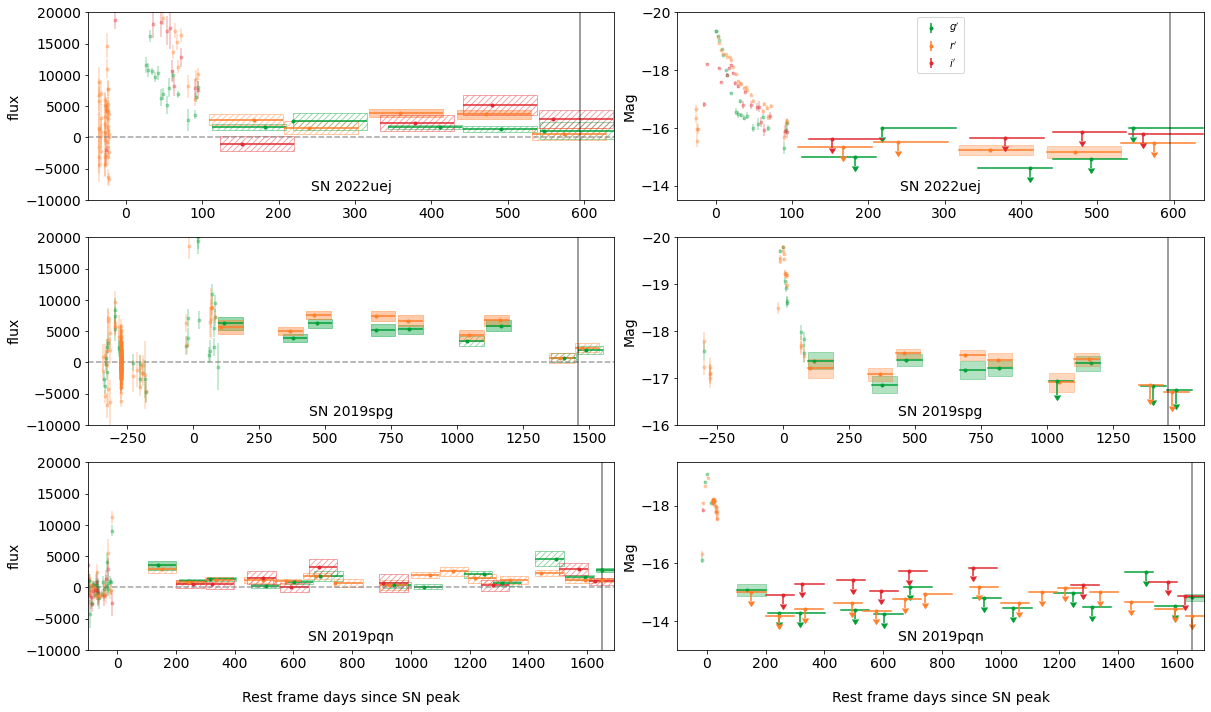
\includegraphics[width=\textwidth]{../Images/chapter_5/non_followup_lcs.png}
    \caption{\textbf{Left:} Binned light curves in flux space in the SN rest frame of the three objects with a late time signal that I could not follow up on. The three ZTF bands \ztfg, \ztfr, and \ztfi\ are shown in green, orange, and red, respectively. Individual observations are shown before the binning starts. Bins are shown as coloured blocks showing the size of the bin, mean value, and $1\sigma$ uncertainty of the binned observations, with the point showing the mean observation date of the bin. Bins that are $>\ 5\sigma$ above zero flux are filled, and bins $\leq5\sigma$ from zero flux are dashed.\\
    \textbf{Right:} Same plot as on the left but in absolute magnitude, corrected for MW extinction. $5\sigma$ detections in individual observations are shown before the binning starts, and the $5\sigma$ binned detections are shown in the same way as in the left plots. $5\sigma$ upper limits are shown with a downward arrow for the binned non-detections. The grey vertical line shows when the excess was first discovered.}
    \label{non_followup_lcs}
\end{figure*}

\textit{\textbf{SN 2019spg.}}
The location of SN 2019spg has a relatively short, sparse baseline before the SN explosion. Immediately after the SN fades, the flux seems to settle at a plateau significantly above the pre-SN baseline. Due to it staying at a nearly constant flux level for much longer than the baseline, this could suggest that the baseline correction was incorrect and the actual baseline should be at the plateau level. With a separation of 0.5$\arcsec$, this object is also very close to the host galaxy nucleus. According to the AGN criterion presented in \citet{WISE_crit}, which uses data gathered with the \textit{Wide-field Infrared Survey Explorer} \citep[WISE,][]{WISE}, the host galaxy is not an AGN. This does, however, not mean that the host cannot show small variability, as has been shown in \citet{Terwel_2024_paper1} and Terwel et al. (submitted). Because of these reasons, I decided not to follow up on this late-time signal. After around 1\,000 days, the flux level dropped again, nearly to the pre-SN baseline level. This drop shows that the previous plateau was a real excess after all, although it was likely related to variability of the host nucleus, not the SN. Due to a combination of unfortunate timing of the excess and unfortunate sampling of the light curve, specifically the pre-SN light curve, these late-time detections of likely nuclear activity looked like a false positive until the signal faded and the original baseline was recovered.

Interestingly, a baseline correction was needed to recover the signal. \textsc{snap} shows no excess in the difference images, but it does show a ghost in the pre-SN region and after the binned signal has faded, which suggests that the excess is in the reference images and that the host dimmed between the time when the reference images were made and the SN explosion.\\


\textit{\textbf{SN 2019pqn.}}
A late-time signal at the position of SN 2019pqn was identified on 28 May 2024, only showing faint \ztfg-band detections that had started 21 days earlier in the rest frame of the SN. This lasted at least 64 days and was active at the end of the monitoring period. Only upper limits in \ztfr- and \ztfi-bands were found at similar epochs. \textsc{snap} shows that the late-time signal lies between the SN and host nucleus locations (which are 1.9$\arcsec$\ apart) but seems to slightly favour the host nucleus location. When this excess was found, I did not have the opportunity to follow it up as I only had very low priority time at the NOT. Therefore, I only have the short period of binned photometry detections. Given that it was only detected in the \ztfg-band, combined with the excess being slightly offset from the SN location, a nuclear transient is a good explanation of this late-time signal, even though the host nucleus is not an AGN according to its WISE colours.


\subsection{Follow-up results}
\label{followups_section}
I found five objects with an active late-time signal for which I could obtain follow-up observations. SN 2019zbq was followed up with the GTC, while the others were followed up with the NOT. Below, I discuss each object individually, starting with the three for which only photometry was taken and then SN 2019zbq, for which I obtained photometry and spectroscopy. SN 2020qxz, for which more extensive follow-up was obtained, is discussed separately in section \ref{sec:SN2020qxz}. The light curves of these objects are shown in Fig.~\ref{followup_lcs}. The details of their follow-up observations are presented in Table \ref{followups}.\\

\begin{figure*}
    \centering
    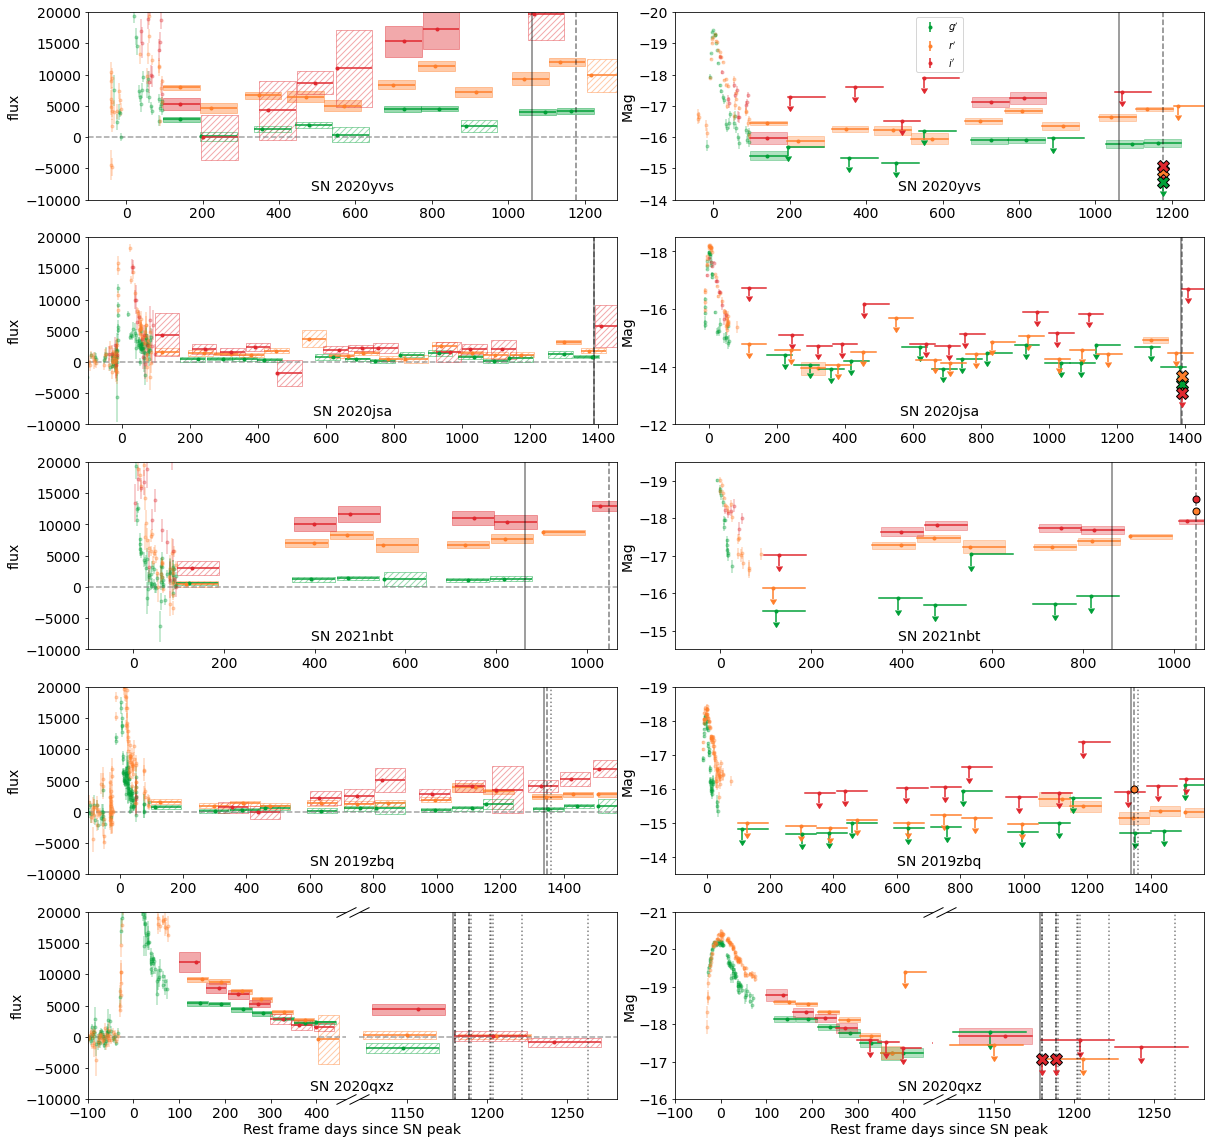
\includegraphics[width=\textwidth]{../Images/chapter_5/followup_lcs.png}
    \caption{Same as Fig.~\ref{non_followup_lcs}, but for the objects for which follow-up observations were made. The grey vertical line shows when the excess was first discovered, and the grey dashed and dotted vertical lines show the photometric and spectroscopic follow-up observations, respectively. The coloured points at the follow-up dates show the follow-up detections and the crosses show the follow-up $5\sigma$ upper limits. Note that for SN 2020qxz the time period between the SN tail and late-time signal has been cut out to better show the detections and follow-up campaign.}
    \label{followup_lcs}
\end{figure*}

\textit{\textbf{SN 2020yvs.}}
On 20 November 2023, SN 2020yvs was found to have elevated flux levels in all three ZTF bands that had started nearly 1\,000 d before, with the effect being stronger in the redder bands. With \textsc{snap} the detected excess is clearly visible, though, at times, it is merged with a residual dipole from the host. As the SN is very close to the bright nucleus of the host galaxy (1.3$\arcsec$, host SDSS \ztfr\ mag = 13.56), I decided to keep a close eye on the development of the light curve to determine if it was more likely to be associated with the SN or not.

As the late-time detections grew stronger over time, I obtained confirmation through photometry with NOT/ALFOSC in the \ztfg\ztfr\ztfi-bands. These observations were obtained on 19 March 2024, with ten exposures of 10 s each using the SDSS \ztfg\ztfr\ztfi\ filters that were stacked together for each band. The short exposures are needed to avoid saturating the host galaxy as image subtraction has to be performed to search for an $\sim 20$ mag excess in an $\sim 13.5$ mag environment. The image subtraction was done through \textsc{autophot} \citep{Autophot} using SDSS images as templates and was attempted using Pan-STARRS images as templates, though these proved to have a saturated host galaxy, making them unusable as templates.

After image subtraction, a small residual at the host nucleus was left, but no excess was found at the SN location. The host residual is the brightest source close to the location, having at most a $2\sigma$ detection at 21.6 mag in the \ztfi-band. This is significantly below the detections found in the late-time ZTF light curve (brighter than mag 20 in both \ztfr\ and \ztfi). Therefore, I conclude that the binned detections are not real but likely due to artefacts in the ZTF images after subtracting the bright host galaxy.\\


\textit{\textbf{SN 2020jsa.}}
The late-time signal in SN 2020jsa was found on 1 May 2024, showing a $21.2\pm0.1$ mag \ztfr-band excess that had begun 112 days earlier and was already fading at the time of discovery. The SN is located 3.0$\arcsec$ from the host galaxy nucleus, and a previous faint detection in the binned late-time light curve can be seen around a year after the SN peak. While the host nucleus is relatively far from the SN, the difference images show a dipole with the positive side towards the SN after host subtraction. This would suggest that there are subtraction issues or that the host shows slight variability. However, according to the WISE criterion, the host galaxy is not an AGN. The object was observed with the NOT in \ztfg\ztfr\ztfi\ the next night, using short exposures to avoid saturation of the bright host and nearby stars. The resulting difference images found no excess at the SN location, providing a deeper limit than the binned ZTF \ztfr-band light curve. However, a faint residual was found at the host nucleus location, showing that the excess is real but unlikely to be related to the SN.\\


\textit{\textbf{SN 2021nbt.}}
The late-time signal in SN 2021nbt was first detected on 5 December 2023. The object is only 0.6$\arcsec$\ from the host nucleus, and its ZTF name is from 2018, which suggests that some host variability caused a first detection long before the SN exploded. This immediately raised suspicion that the detected late-time signal could be related to the host instead. Because of this, it took until 21 June 2024 before I decided to follow it up with the NOT. The signal started relatively shortly after the SN and persisted for several months, which could suggest it is connected to the SN in some way.

After difference imaging was performed on the \ztfr\ztfi-band photometry obtained with the NOT (see Table \ref{followups}), a residual was recovered at \ztfr\ $= 19.458\pm0.040$ mag and \ztfi~$= 19.123\pm0.062$ mag. This is somewhat brighter than the binned detections using ZTF observations taken around the same time, and a signal this bright would have been detectable in the individual ZTF observations. If the host nucleus varies slightly over time, however, this could cause different reference images to show the host at different brightness, which would result in different residuals after difference imaging. Unfortunately, there is no spectrum of the host galaxy, and since the signal is superimposed on the much brighter host, it is impossible to extract a spectrum of the excess without it being completely dominated by the host. The host is too small to attempt extracting a pure host spectrum away from the excess location, and without a host spectrum, the excess contribution cannot be isolated.

At the distance of the host, the magnitude of the excess observed by the NOT translates to an absolute magnitude of M $\sim -18$ mag. As can be seen in Fig.~\ref{followup_lcs}, the excess appears after a gap in the observations and persists for at least 780 days at a fairly constant magnitude. This is at the bright end of the potential ambiguous nuclear transient \citep{2020ohl_Hinkle} population identified in Terwel et al. (submitted), but still consistent with the brightness of the comparison object they use. Due to its shape, brightness, and duration, an ANT that started somewhere between 200 and 400 days after the SN is a good explanation for this excess. However, I do not have spectroscopy to confirm since it was so faint relative to the host.\\


\textit{\textbf{SN 2019zbq.}}
On 13 November 2023, SN 2019zbq was noted to have an active late-time signal in the binned \ztfr-band at m $=21.5\pm0.2$ mag, with the signal already being present for nearly 300 days before and being recovered regardless of bin size or placement. The binned \ztfg-band did not rise from the baseline during this time, but the \ztfi-band did, though the larger uncertainties in this band prevented the detections to reach a $5\sigma$ confidence level. The SN is close to the centre of its host galaxy, with an offset of $1.09\arcsec$.

Checking the \ztfr-band difference images with \textsc{snap} ruled out image defects, reduction or subtraction errors, or a sibling transient with a small sky separation from SN 2019zbq (within the uncertainty of the ZTF resolution) as potential explanations for the detections. The host galaxy has \textit{W1 -- W2} = $0.02\pm 0.04$ and  \textit{W2 -- W3} = $0.9\pm 0.5$, which is not an AGN according to the AGN criterion presented in \citet{WISE_crit}.

\ztfr-band image was obtained with GTC+OSIRIS+ on 23 November 2023. Using \textsc{autophot} and reference images from Pan-STARRS, a m $=20.7\pm0.1$ mag source at the host nucleus location was obtained, which is clearly offset from the SN location, confirming the late-time excess is real but not related to the SN. The GTC image and the resulting difference image are shown in fig.~\ref{2019zbq_difim}.

\begin{figure}
    \centering
    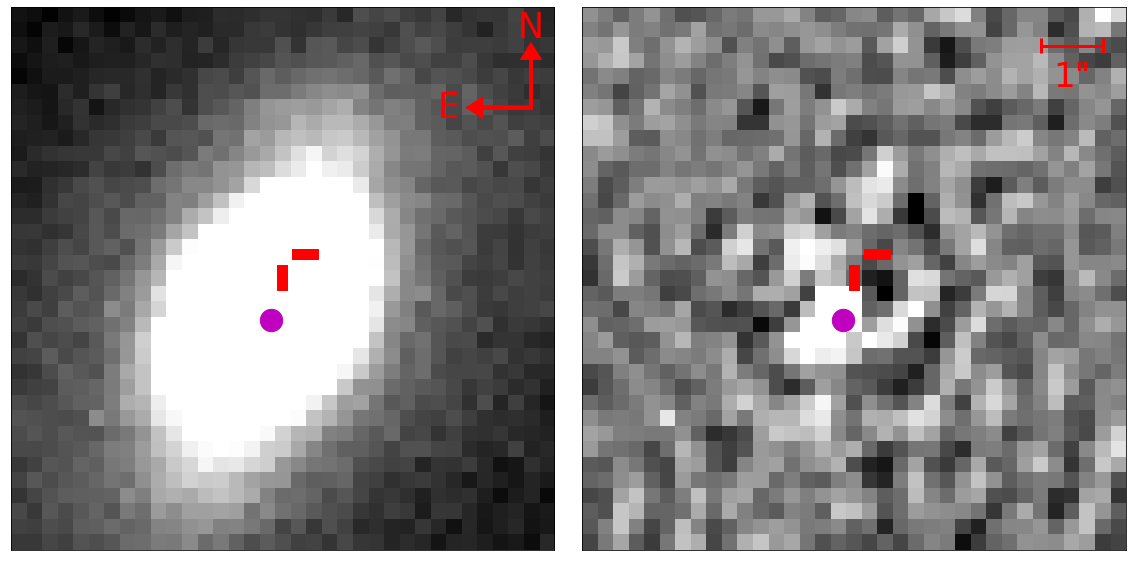
\includegraphics[width=\textwidth]{../Images/chapter_5/2020zbq_difim.png}
    \caption{\textbf{Left:} \ztfr-band image of the location and host galaxy of SN 2019zbq, taken on 23 November 2023 with GTC+OSIRIS+. The SN location is marked in red and the purple dot is the galaxy nucleus location. \textbf{Right:} Difference image of the left region after subtracting a Pan-STARRS template image. There is a residual visible at the host galaxy location. Note that the colour scaling is different for the two images to highlight the important sources.}
    \label{2019zbq_difim}
\end{figure}

On 4 December 2023, a spectrum was obtained with the GTC and OSIRIS+. Since the transient is located on top of the host, this spectrum contains light coming from both the host and the transient. The host is 4.5 mag brighter and dominates the spectrum heavily, meaning the host must be subtracted to recover any potential transient spectrum. Since a slit was used in obtaining the spectrum and the host galaxy is an extended object, A pure host galaxy spectrum is extracted away from the transient location, and I subtract it from the spectrum at the brightest part of the trace containing the transient. Assuming that the spectral features of the host are similar enough at these two locations, the main difference between the two, apart from total flux observed, will be the excess I am interested in.

\begin{figure*}
    \centering
    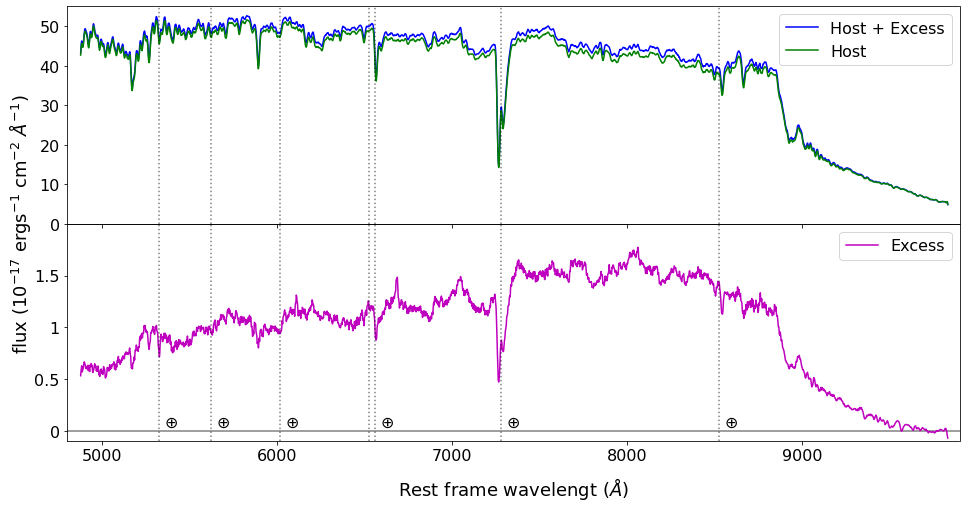
\includegraphics[width=\textwidth]{../Images/chapter_5/2020zbq_spec.png}
    \caption{GTC spectrum of the transient in the SN 2019zbq host galaxy, taken on 4 December 2019. Vertical dotted lines give the locations of sky lines and tellurics. \textbf{Top:} Extracted spectra at the centre of the trace (host + excess) and at the side of the extended host galaxy trace (host). \textbf{Bottom:} The difference of the two spectra in the top panel, showing the isolated spectrum of the excess. The host spectrum has been re-scaled to ensure that the red edge is the same for both spectra.}
    \label{2019zbq_spec}
\end{figure*}

Figure~\ref{2019zbq_spec} shows the extracted host and excess spectra. Since the red edge of the detector has very low sensitivity, this can be used to scale the pure host spectrum to the combined host and excess spectrum, allowing me to take the difference and extract the pure excess spectrum. The pure excess spectrum is shown in the bottom panel. Integrating this spectrum over the \ztfr-band shows this excess to be $\sim21$ mag, which agrees with the photometry values. A few small spikes can be seen in the excess spectrum, but these do not match up with any known emission lines at the host redshift, even when assuming a consistent velocity offset of the excess from the host. Overall, the spectrum looks red, which matches the binned ZTF data, as the \ztfg-band does not rise from zero flux (and the \ztfi-band rises the most but with a large scatter).\\

The excess has an absolute magnitude M $=-16.0$ mag. This, together with the nuclear location and the sudden appearance of the transient followed by a relative stable plateau for over 500 days, is consistent with the faint ANT-like nuclear transients found in Terwel et al. (submitted). Therefore, I conclude that a faint ANT-like transient provides a good explanation for the signal, although I caution that extracting the transient spectrum and removing the host contribution is not straightforward.

\subsection{SN 2020qxz}
SN 2020qxz was classified as a SN Ia-CSM at early times, with a prominent \Halpha\ line visible in the classification spectrum taken around the SN peak, which was used to obtain a redshift of $z=0.0964$ for the object. The slowly decaying tail is visible in the ZTF observations up to 1.2 years after the peak and an additional three months in the binned light curve before fading below the noise limit, resulting in its recovery in \citet{Terwel_2024_paper1}.

On 20 March 2024 (mjd 60389), at nearly 1\,180 d after the SN peak in the rest frame, this object was flagged as currently active due to an elevated flux level in the \ztfi-band in the last four weeks, with the detection being at m $=20.9\pm 0.2$ mag (see bottom row of Fig.~\ref{followup_lcs}). As can be seen in Fig.~\ref{2020qxz_loc}, the SN location is visually offset from the host galaxy, so I obtained follow-up observations with the NOT+ALFOSC on the same night (20 March 2024). The resulting spectrum showed a prominent emission line around $\lambda=9\,210$ \AA\ in the observer frame ($\lambda=8\,400$ \AA\ in the SN rest frame). After this promising detection, I launched a campaign to take more observations (photometry and spectroscopy) with the NOT+ALFOSC over the following weeks.


\subsubsection{Late-time photometry}
Two epochs of \ztfi\ photometry were taken with the NOT+ALFOSC on 20 and 30 March 2024. Both were single 600 s exposures, which were reduced using the method described in section \ref{sec:reduction}. No residual flux above $5\sigma$ was found in either image, resulting in m~=~21.5~mag upper limits. As can be seen in Fig. \ref{followup_lcs}, all observations taken with the NOT were after the detection in the binned ZTF data. However, likely transient flux was detected in the spectra taken at the same epochs as this follow-up photometry. The most likely explanation for the photometric non-detections at the same epochs is that the emission lines seen in the spectra are no longer strong enough to cause a detectable increase in the broadband flux. 

\label{sec:SN2020qxz}
\begin{figure}
    \centering
    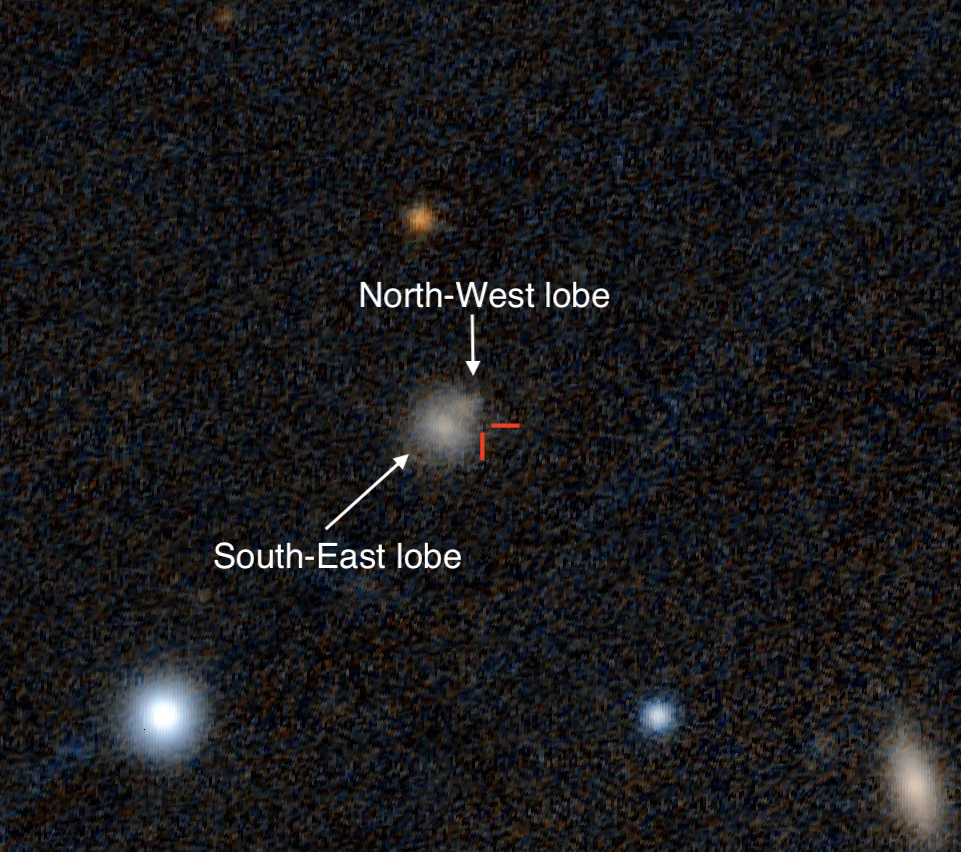
\includegraphics[width=\textwidth]{../Images/chapter_5/2020qxz_loc.png}
    \caption{Pan-STARRS DR1 colour image of the location and host galaxy of SN 2020qxz. The SN location is marked in red, and the two host galaxy lobes are marked in white.}
    \label{2020qxz_loc}
\end{figure}


\subsubsection{Host spectroscopy}
\label{2020qxz_host_specs}
\begin{figure*}
    \centering
    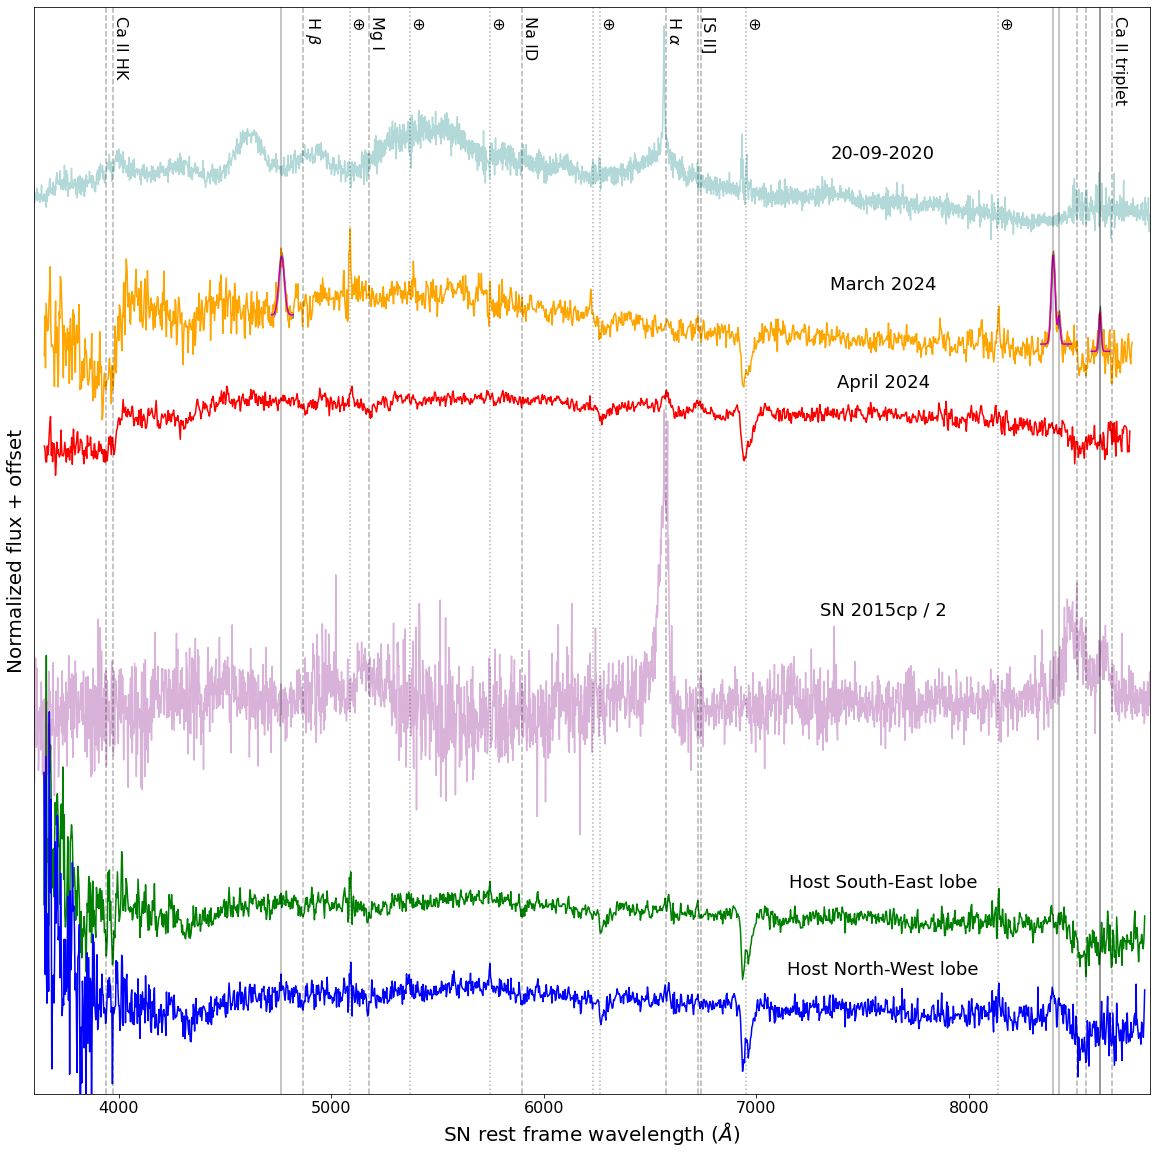
\includegraphics[width=\textwidth]{../Images/chapter_5/2020qxz_spec.png}
    \caption{Combined late-time spectra of 2020qxz and its host in the SN rest frame. The transient emission lines are marked with grey vertical lines, and the best-fit Gaussians are overlaid on top of the combined March spectrum. The dashed vertical lines show the location of host galaxy lines (as well as \Hbeta\ to compare its location to the transient emission line) at the host redshift of $z=0.0975$, and the dotted vertical lines show the location of sky lines. I also show the classification spectrum of SN 2020qzx taken around peak magnitude in light blue and the late-time spectrum obtained for SN 2015cp in magenta, scaled down by a factor of 2 for readability.}
    \label{fig:2020qxz_spec}
\end{figure*}

\begin{figure*}
    \centering
    \includegraphics[width=\textwidth]{../Images/chapter_5/2020qxz_spec_zoom.png}
    \caption{Same as Fig~\ref{fig:2020qxz_spec} but zoomed in on the regions containing the transient emission lines and the \Halpha\ region. The $1\sigma$ uncertainties of the Gaussian fits are shown in grey.}
    \label{2020qxz_spec_zoom}
\end{figure*}

The host galaxy of SN 2020qxz has two lobes, a big one on the South-East side and a smaller one on the North-West side (see Fig.~\ref{2020qxz_loc}). By orienting the slit along the axis of the galaxy, I obtained spectra of both lobes on the nights of 3 May and 19 June 2024 with the NOT+ALFOSC, resulting in a two-hour spectrum on the big (South-East) lobe and a one hour and 40 minutes spectrum on the small (North-West) lobe as one of the 20-minute exposures on 3 May 2024 was contaminated at the location of the small lobe and could not be used.

The spectra of the big and small lobes shown at the bottom of Fig.~\ref{fig:2020qxz_spec} look nearly identical, and the galaxy emission and absorption lines discussed below are at the same position for both lobes. This shows that the host is more likely a single object at a single $z$ rather than two distinct galaxies overlapping in the line of sight.

Several lines can be seen in the host spectra. I identify weak lines which I associate with \Halpha\ emission, \SIIF\ emission, \CaII\ H\&K, and NIR triplet absorption, and \NaID\ and \MgI\ absorption. These galaxy lines match the spectrum at $z=0.0975$, which is slightly higher than was found for the \Halpha\ emission seen in the maximum-light classification spectrum of SN 2020qxz as Ia-CSM (top spectrum in Fig.~\ref{fig:2020qxz_spec}). Assuming that the host galaxy is indeed at this higher $z$ and that the SN is associated with the host and at the same $z$, the blueshifted \Halpha\ line in the classification spectrum of SN~2020qxz translates to the SN moving towards us with $\sim200$ km s$^{-1}$ with respect to the host galaxy. The different $z$ value would also slightly change the distance modulus, resulting in all absolute magnitudes being increased by $\sim0.03$ mag. Unless specified otherwise, I use the SN rest frame at $z=0.0964$ while further discussing this object.


\subsubsection{Late-time spectroscopy at the SN location}
\label{2020qxz_spec}
I obtained spectra at several epochs at the position of SN 2020qxz in March and April 2024, which were combined into a `March' spectrum and `April' spectrum (see section \ref{sec:reduction} for further details). In the March spectrum, I identify four prominent emission lines and zero absorption lines that are not associated with the host galaxy. Both the March and April spectra show some signs of slight host contamination, but the four emission lines are only seen in the March data, not in the April spectrum nor the host spectra obtained in May and June 2024. This suggests that these features are transient in nature, and are decaying between the two periods of observations. These emission lines are seen at $4\,766.0\pm1.1$ \AA, $8\,395.8\pm0.6$ \AA,  $8\,423.6\pm1.4$ \AA, and $8\,615.8\pm1.3$ \AA\ in the rest frame of the SN and are marked in Fig.~\ref{fig:2020qxz_spec} and Fig.~\ref{2020qxz_spec_zoom}.

I have fitted these four emission lines with Gaussian profiles to measure their strengths and widths, the results of which are given in Table~\ref{fitres_2020qxz}. The fits to the four lines are shown in Figs.~\ref{fig:2020qxz_spec} and~\ref{2020qxz_spec_zoom}. Three of the lines have a similar dispersion, suggesting that they are from the same source. However, the bluest line has a much higher dispersion that is incompatible with the other three.

\begin{table*}[]
    \centering
    \caption{Line fits for the emission lines identified in the March 2024 spectrum at the position of SN 2020qxz. The first three columns give the central wavelength and width (in \AA\ and km s$^{-1}$) of the fitted lines. The last three columns give the most likely matched elements and emission lines, assuming some amount of blueshift velocity offset (given in the last column). The redshift uncertainty contribution to the velocity offset ($120$~km~s$^{-1}$) has not been included. All fits are done in the SN rest frame.}
    \resizebox{\textwidth}{!}{
    \begin{tabular}{ccc|ccc}
        \hline
        \hline
        Central wavelength (\AA) & $\sigma$ (\AA) & $\sigma$ (km s$^{-1}$) & Element & Rest wavelength (\AA) & Velocity offset (km s$^{-1}$)\\
        \hline
        4\,766.0 $\pm$ 1.1 & 12.7 $\pm$ 1.4 &  800 $\pm$ 88 & \Hbeta & 4\,861.00 & $5\,920\pm70$\\
        8\,395.8 $\pm$ 0.6 & 9.3 $\pm$ 0.7 &  332 $\pm$ 25 & \CaII\ $^{(1)}$ & 8\,542.00 & $5\,180\pm20$\\
        8\,423.6 $\pm$ 1.4 & 5.6 $\pm$ 1.5 &  199 $\pm$ 53 & \NI & 8\,567.74 & $5\,090\pm50$\\
        8\,615.8 $\pm$ 1.3 &5.8 $\pm$ 1.5 & 202 $\pm$ 52 & \KI\ $^{(2)}$ & 8\,763.96, 8\,767.05 & $5\,170\pm50$ \\
        \hline
    \end{tabular}
    }
    \begin{flushleft}
        $^{(1)}$ Only the middle line of the \CaII\ NIR triplet is visible, the other two lines are not present due to atmospheric and host contamination for the blue and red component, respectively.\\
        $^{(2)}$ \KI\ is a doublet for which I use the mean to estimate the velocity offset.
    \end{flushleft}
    \label{fitres_2020qxz}
\end{table*}

Identification of the origin of these emission lines is not straightforward. SN~2020qxz is a known SN Ia-CSM that showed \Halpha\ emission near peak brightness, so it is natural to assume that at least one of the four lines in the March 2024 spectrum is due to H emission. Indeed, the line at $4\,776$ \AA~can be interpreted as \Hbeta\ emission, though this requires it to be blueshifted by $5\,920\pm70$ km s$^{-1}$. Offset emission lines have been found before at up to 10\,000 km s$^{-1}$, see e.g., \cite{2019bkc_Chen} and \cite{2019bkc_Prentice}. However, the significant difference in the hydrogen velocity between the early and late-time detections suggests that this material has been accelerated in the time between detections or is coming from a different location.

SN ejecta sweep up the CSM they are interacting with, so some acceleration can be expected. This has been seen before in some SNe IIn, where aspherical, possibly clumpy CSM has been accelerated to several thousand km s$^{-1}$ resulting in wide boxy or multi-peaked emission lines \citep{1998S_aspherical_CSM, 1998S_late-time, PTF11iqb}. The other issue is that where there is \Hbeta\ emission, one would expect \Halpha\ emission as well. However, there is no sign of any emission line at the position of \Halpha\ in the March or April spectra. There is a small bump that is consistent with being due to host \Halpha\ contamination, but nothing is seen with the same offset as \Hbeta.

The other three transient emission lines at 8\,395.8 \AA,  8\,423.6 \AA, and 8\,615.8 \AA\ in the rest frame of the SN  have their own identification challenges. First of all, these are in the same region as the host galaxy \CaII\ NIR absorption. For the transient emission lines to be visible, this dip in the background spectrum has to be overcome first. Three emission lines are found, but their relative positions are different from the \CaII\ NIR triplet, meaning that not all lines can be explained by them. If I however shift the middle line of this triplet to match with the bluest transient line, the blue line in the \CaII\ NIR triplet overlaps with a skyline while the red line is in the middle of the dip mentioned before. This could explain why only one of the three components is visible. The required blueshift is $5\,180\pm20$ km s$^{-1}$, significantly lower than the shift required for \Hbeta\ of $5\,920$ km s$^{-1}$. A shift of $\sim5\,150$ km s$^{-1}$ allows the remaining two transient lines to be matched to a \NI\ line and \KI\ doublet with the same velocity, resulting in a possible identification of three offset emission lines with similar widths. For the emission line matching with the \KI\ doublet I use the mean wavelength.

Neither of these elements are expected to have a strong presence in the ejecta of SNe Ia, nor have these lines been seen in other SNe with CSM. \citet{2014J_KI} did, however, find time-varying \KI\ absorption lines in SN 2014J around its peak, which they associate with photoionization of distant CSM, although the inferred distance is larger than what the ejecta could travel in a couple of years. It might also be possible to obtain a nitrogen-enhanced CSM if the donor star is an evolved star massive enough to burn hydrogen through the CNO cycle but small enough for the primary to have ended up as a WD. Dredge-ups could bring fusion products to the surface, including nitrogen, which is then lost from the system to form the CSM. \citet{N_lines_SECCSN} make a similar argument for the production of [\NII] lines in stripped envelope CCSNe.

The late-time CSM in SN 2015cp was primarily \Halpha\ dominated \citep{2015cp}, which is absent in SN 2020qxz. At the same time, three of the four emission lines found in SN 2020qxz are absent in SN 2015cp. There is a tentative detection of the \CaII\ NIR triplet in SN 2015cp, but unlike in SN 2020qxz, all three components are observed. They only require a velocity offset of $\sim1\,400$ km s$^{-1}$, though with a FWHM of $\sim3\,000$ km s$^{-1}$ the \CaII\ lines in SN 2015cp are much broader than any of the transient emission lines found in SN 2020qxz.


\section{Discussion}
\label{discussion}
In this study I monitored a sample of 6\,914 SNe Ia discovered by ZTF for signs of late-time rebrightening due to potential CSM interaction. I created forced photometry light curves at the location of each SN for the full duration of the survey and updated these every four weeks with the latest observations in an attempt to find late-time signals in real time and follow them up with further observations. I found 12 objects with late-time rebrightening that could not be explained by image defects, known contamination of host nuclei, or known sibling transients. Four of these were known from \citet{Terwel_2024_paper1} and discussed there. Their rediscovery here did not lead to any new insights. In three objects, the signal was found when follow-up was not possible. I was able to follow the signals in the other five objects up, using the NOT for four objects and the GTC for one. Out of these, there was one false positive, three likely nuclear transients unrelated to the SN, and a confirmed late-time signal in SN 2020qxz.


\subsection{Detection challenges}
As was shown in \citet{Terwel_2024_paper1} and Terwel et al. (submitted), late-time signals in SNe Ia are rare. Out of nearly 7\,000 objects, I found eight objects with a late-time signal detected somewhere in the 240 days as I was actively monitoring them and an additional four objects whose late-time signals were already discussed in \citet{Terwel_2024_paper1}. During this time many other objects were flagged but turned out to be false positives, bright long-lived SNe, or sibling transients. SNe near their host nucleus are especially prone to give false detections.

Most objects for which a late-time signal was flagged in Table~\ref{found_objs}, \citet{Terwel_2024_paper1}, and Terwel et al. (submitted) are close to the host nucleus. These regions are difficult to handle with difference imaging, often leading to residuals that can be mistaken for a weak signal by forced photometry. Even if the excess is real, the busy centres of galaxies leave plenty of opportunity for alternative explanations, including ones involving the central supermassive black hole such as AGN, tidal disruption events and other sources of nuclear variability, e.g. ANTs \citep{2020ohl_Hinkle}. One could make a cut on the host separation to ensure that contamination from nuclear events is removed, but I did not do this here as it would introduce a bias in the SN environments in my sample. Such a cut is also dependent on the pixel size of the used observations, which means that more distant SNe require larger host separations in order to not be removed by the cut. I decided to instead be as inclusive as possible with the knowledge of the contamination this leads to in my results.

Even when searching for faint late-time signals in real time, the fact that my method requires several observations to bin together in order to reach a deeper detection limit results in my method still being slightly behind current events. This makes it crucial to follow up quickly on newly found signals with bigger telescopes and better instruments that are able to measure such faint signals, especially as sometimes the late-time signals have been relatively short-lived and were already fading again by the time they were found. Without my ability to follow up quickly, the transient emission lines in SN~2020qxz might have been missed.


\subsection{Follow-up campaigns}
For five objects that showed late-time signals, I was able to get follow-up photometry, on which difference imaging and forced photometry was performed using \textsc{autophot}. In one case (close to the position of SN 2020yvs), the follow-up observations provided deeper non-detections than the late-time signal that was found in the binned ZTF observations. The host galaxy of SN 2020yvs is very bright, which likely results in small artefacts in the difference images that are misidentified as the late-time signal. In three other cases (close to the positions of SNe 2020jsa, 2021nbt and 2019zbq), a residual was detected at the host nucleus location, showing that for these objects the recovered late-time signal was unrelated to the SN.

The host galaxy of SN 2019zbq was confirmed to have an active nuclear transient and was followed up with spectroscopy. However, since the host galaxy is 4.5 mag brighter than the transient, it dominates the spectrum heavily, and the only way to extract the transient spectrum is by subtracting the host contribution. This requires the existence of a pre-transient host spectrum (from e.g. SDSS, as was done for the late-time signal in SN 2020alm in \citealt{Terwel_2024_paper1}) or a host spectrum without contribution from the transient extracted from the same observation as the spectrum containing the transient, as was done for SN 2019zbq in section~\ref{followups_section}. This is a tricky process and can introduce a lot of uncertainty. For this reason, I did not attempt to get a spectrum of the confirmed excess in the host of SN 2021nbt, as there was already enough evidence of the late-time excess being unrelated to the SN. Integrating the flux of the SN 2019zbq host excess spectrum over the \ztfr-band matches the measured \ztfr-band brightness, showing that the excess extraction has worked.

The excess spectrum in the SN 2019zbq host looks quite red but has no distinctive emission or absorption features. This is similar to the ANT AT 2020ohl \citep{2020ohl_Hinkle}, although AT 2020ohl is much bluer and brighter. The ANTs presented in \citet{wiseman_ztfants} are much closer to the excess in colour but again much brighter, and they all show Balmer emission lines. The small peaks that do stand out in the excess spectrum do not match any set of elements at a single velocity offset. The best I can say about it is that this is indeed some sort of ambiguous nuclear transient.


\subsection{The late-time signal in SN 2020qxz}
\label{2020qzx_discussion}
SN 2020qxz stands out from the other objects in the sample for several reasons. First of all, it is a SN Ia-CSM with detected interaction around its peak. It is also visually separated from its host nucleus, which makes it easier for the excess to be interpreted as being related to the SN instead of nuclear activity, and it is also easier to get a spectrum of the excess without much contribution from the host galaxy. I followed this excess up over three months and obtained nearly six hours of spectroscopic data of the transient, which I combined into a March spectrum and an April spectrum. I also got a spectrum of the two lobes of the host galaxy to confirm that they are not two galaxies overlapping in the line of sight and finding a host redshift of $z=0.0975$. This is slightly higher than the estimated $z=0.0964$ from the \Halpha\ line in the SN peak spectrum, and gives the SN a velocity of $\sim200$ km s$^{-1}$ with respect to the host galaxy. The SN is 3.4$\arcsec$\ from the centre of the South-East lobe, which translates to 7~kpc at the host redshift. This means that the SN velocity can be interpreted as its rotation velocity around the host.

The March spectrum shows four emission lines that are not in the host spectrum, and these had disappeared a few weeks later in the April spectrum. The transient nature of these lines shows that they are associated with the \ztfi-band detection in the binned ZTF light curve. As the follow-up was performed when the late-time signal was already fading again, both the photometric follow-up and the binned observations resulted in non-detection during the follow-up campaign. The remaining transient emission lines are too faint to be picked up in the broadband photometry and are only found during the long spectroscopic observations. This suggests that I only managed to obtain the tail end of the identified signal with spectroscopy.

The only way to match the transient emission lines to elements that can be expected in such an environment is to allow for a large velocity offset. The three lines around 8500 \AA\ all require a velocity of $\sim5\,150$ km s$^{-1}$, matching them with one of the lines of the \CaII\ NIR triplet (the other two are likely contaminated by the host lines, see section \ref{2020qxz_host_specs}), \NI, and \KI\ emission lines. Fitting the lines with Gaussians shows they have similar widths, suggesting that the elements producing these lines are in the same location. The bluest transient line, however, is best matched by \Hbeta\ with an offset of $5\,920\pm70$ km s$^{-1}$. It is also broader than the other three lines. This suggests that, if this line identification is correct, the H-rich material is in a different and faster moving cloud than the N, K, and Ca. It is important to note that although I did not use an order-blocking filter for these observations, none of the emission lines match a second-order diffraction of another emission line, showing that they are four different emission lines.

One problem with the interpretation of the emission line as being \Hbeta\ is that in most cases, when \Hbeta\ is detected, one would also expect to detect \Halpha\ with at least the same strength. This is not the case here, nor is there any sign of an absorption feature at the expected location of \Halpha\ that could completely wipe out a strong, relatively broad emission line like this. However, identifying this line as another element requires a very different velocity and leaves the open question of its strength and width, making \Hbeta\ the best match despite its shortcomings.

The classification of SN 2020qxz as a SN Ia-CSM is due to the \Halpha\ signal around the SN peak from interaction with CSM relatively close to the progenitor system. The late-time signal suggests a second region of CSM further from the progenitor system. Assuming that the inner CSM has a shell or torus-like structure, the interaction signature has the same total redshift as the SN. The late-time transient lines require a significant velocity offset, and their Gaussian profiles were much wider than that of the \Halpha\ line. This shows that the outer CSM is moving much faster and has much more of a patchy structure. Velocity offsets of a few thousand km s$^{-1}$ have been seen before \citep{Maeda_exp_asymetry, Maguire_opt_NIR}. While $>5\,000$ km s$^{-1}$ is high, it is not unprecedented, as the \CaII\ lines in SN 2019bkc have been meaured to be up to $10\,000$ km s$^{-1}$ \citep{2019bkc_Chen, 2019bkc_Prentice}.

CSM with velocity offsets in this regime has been seen before in some SNe IIn. It has been interpreted as material that has been accelerated as it has been swept up. If the CSM is clumpy or disk-like, this can result in a multi-peaked emission line where the redshifted peak is weakened as it comes from the receding end of the SN and has had to travel through dust-forming SN material \citep{1998S_aspherical_CSM, 1998S_late-time, PTF11iqb}. In the case of SN 2020qxz, this could be interpreted as the ejecta running into a shell of H-rich CSM around peak light, resulting in the \Halpha\ line in the classification spectrum. As the CSM is swept up, it is accelerated to at least $\sim6\,000$ km s$^{-1}$ before a part of the accelerated ejecta crashes into a cloud of CSM, resulting in the interaction signal that was observed in 2024. Only the expanding part of the ejecta with accelerated CSM that interacts with this CSM cloud would be emitting light, explaining the offset. However, the viability of such a scenario needs proper modelling.


\section{Conclusions}
\label{conclusion}
In this work I have presented a real-time search of late-time signals in 6\,914 Type Ia SNe in ZTF, using the latest observations to create the most up-to-date light curves for the objects in my sample. By binning the latest observations I was able to go up to nearly one magnitude beyond the single observation limit, which allowed me to find eight new faint signals during the 240-day monitoring effort. Using the NOT and GTC, three of these objects were subsequently followed up with photometry, and two objects were followed up with photometry and spectroscopy. My main conclusions are:

\begin{enumerate}
    \item The requirement to bin observations to get deeper magnitude limits makes even the most real-time strategy lag slightly behind current events. In some cases this resulted in the discovery of a (short-lived) late-time signal while it was already declining again. Quick follow-up is required, but only the tail end of the signal can likely be observed.
    \item Late-time signals are rare, and detections of late-time signals that are associated with the SN are contaminated with detections of associated objects in the same line of sight. This is more prevalent for SNe in or close to the centres of their host galaxies.
    \item In five objects, the late-time detections have been determined to be due to nuclear activity. One of these was not followed up on as it was initially dismissed as a false positive until it faded. This shows the importance of a good baseline when searching for faint signals. The three objects that were followed up showed an excess at the location of the host nucleus, clearly separated from the SN position due to the better resolution.
    \item The excess in the SN 2019zbq host was followed up spectroscopically and showed both similarities and differences to previously studied ANTs, with the main difference being the absolute magnitude of the signal. Since the excess is 4.5 mag fainter than the host nucleus, extracting its spectrum required careful subtraction of the host signal, which complicates studying faint ANTs like these.
    \item The late-time signal in SN 2020qxz stood out from the others, as this is a SN Ia-CSM at $\sim7$ kpc from the host nucleus, making it significantly easier to follow up. While the signal was short-lived, I was able to follow it up spectroscopically, finding four transient emission lines that are best matched by four different elements at two different but highly blueshifted velocities ($5\,150 - 5\,920$ km s$^{-1}$). This suggests that the progenitor system created at least two regions of CSM, one nearby that resulted in the initial Ia-CSM classification and one further away that resulted in the late-time signal.
\end{enumerate}

Faint late-time signals in SNe Ia due to interaction with distant CSM are rare, and even with techniques like binning observations to reach the deepest detection limits, only the brightest and strongest signals can be detected with current surveys. The upcoming Vera C.~Rubin Observatory's Legacy Survey of Space and Time \cite[LSST;][]{LSST} will be able to detect objects several magnitudes deeper than ZTF, allowing the detection of fainter objects in a larger volume. Monitoring existing SN samples like those found by ZTF with LSST will be the best way to find faint late-time signals, which could then be followed up spectroscopically to find the chemical composition of the source of the signal. Constraining the properties of these rare events will allow us to probe the physics that govern SN Ia explosions more thoroughly and gain new insights to help explain them.

\end{document}
%!TEX root = ../main.tex
\documentclass[a4paper,oneside,12pt, class=Latex/Classes/PhDthesisPSnPDF, crop=false]{standalone}
\usepackage{setspace}
\begin{document}
\doublespacing
\chapter{Conclusions and future work}
\label{chap:Conc_and_fut}

In this thesis I have presented my work on the search for signs of interaction between the ejecta of SNe Ia and distant CSM. Due to the distance of the proposed CSM the interaction would start at late times, which I defined to be $\geq100$ days after the observed SN peak in the observer frame, and cause an extreme flattening or rebrightening in the SN light curve. I searched through three different samples of objects, these being the ZTF SN Ia DR2 (section \ref{chap:DR2_search}), transients that were first detected between 2008 and 2018, including objects that were not SNe Ia (section \ref{chap:pre-ZTF_search}), and a real-time search using all SNe Ia discovered by ZTF up to July 2023 in order to follow candidates up using the NOT and GTC (section \ref{chap:Real-time}).

To conduct this search in a systematic manner and to be able to recover the faintest signals hidden within the data, I built a custom analysis pipeline, which is presented in section \ref{pipeline} and tested through a simulated observing campaign in section \ref{simulation}. After an initial cleaning and calibration of the data, the late-time observations were binned together in bins with a size between 25 and 100 days. By doing so, I was able to push the detection limit beyond that of the individual observations, near the noise limit of the reference images used by ZTF in their difference imaging pipeline. This was done separately for the different ZTF bands \ztfg\ztfr\ztfi.


\section{Conclusions}
Searching through these three samples made one thing abundantly clear: late-time CSM interaction in SNe Ia is very rare, and the only way to systematically find them is by searching through large data sets, preferably catching them while they are active so they can be followed up on. By doing so, it will be possible to study properties of the CSM, such as its size and composition, gain new insights in SN Ia explosions and the physics that governs them, and place constraints on their progenitor systems. Based on the work I presented, my main conclusions are:

\begin{enumerate}
	\item Across the three samples I analysed, the late-time data consisted of 12\,601 unique spectroscopically confirmed Type Ia SNe, and an additional 3\,089 transients in the pre-ZTF sample that were not classified as SN Ia or one of its subclasses. For some of these transients the data extended up to 15 years after they were first discovered. Out of these, I identified seven candidate objects showing signs of possible late-time CSM interaction, with the first detection of their late-time signal being between 250 and 2\,200 days after discovery in the SN rest frame. Additionally, SN 2020qxz was spectroscopically confirmed to have a period of rebrightening around 1\,150 days after peak light in the SN rest frame.
	\item The largest fraction of objects that are flagged by the pipeline are false positives that show spurious detections in their binned light curves. This is a result of the wide net it casts in an attempt to minimize the chance of missing a faint signal. The visual inspection of these light curves, as well as inspecting the difference images using \textsc{snap}, showed that in most cases the spurious detections are either due to image issues (e.g., in a difficult environment) or due to software issues (e.g., imperfect image subtractions).
	\item Another large group of objects that were flagged by the pipeline are bright nearby SNe, whose declining tail could still be recovered in the bins. Despite attempting to filter for these cases, some slipped through due to gaps in the observations or a tail that did not follow the simple decline model used in the test. These included most known SNe Ia-CSM in the sample and several very nearby objects whose decline displayed a kink around a year after the peak due to a change in their opacity.
	\item I also recovered over a dozen pairs of sibling transients, two transients at (nearly) the exact same location. In one case, this is a line-of-sight effect, with AT 2018iml likely being a CV in the foreground of SN 2009hz. The other cases were sibling SNe occurring in the same galaxy. Some of these were already known, with both siblings already having been classified. In other cases, a possible but unconfirmed (extinct) sibling transient fits the late-time signal. While such sibling transients are not a very common occurrence, modern surveys discover enough new transients that these rare events can be found regularly.
	\item Most objects with a late-time signal that was not easily recognized as a false positive, SN tail, or sibling transient, were close to or on top of the nucleus of their host galaxy. These are difficult and busy environments, and even if the nucleus is not active, there is a lot of room to interpret a late-time signal as something related to the host nucleus instead. One class of possible contaminants I considered are ANTs, ambiguous nuclear transients that do not really fit in the AGN or TDE classes. The objects I recovered are broadly consistent but generally fainter than most known ANTs, suggesting the existence of a previously unknown population of faint ANTs.
	\item Transients that were first detected before the start of ZTF but still visible after the survey started were never properly detected by ZTF, as they are in the reference images that were made shortly before the survey started in March 2018. As a result of this, difference imaging will leave a ghost, a negative imprint that is easily identified using \textsc{snap} (see section \ref{snap}). Forced photometry still works, but the measured flux will be too small or even negative. Through a proper baseline correction, as is done at the start of my pipeline, these objects can still be recovered. AGN and variable stars can be recovered in the same way, though a proper baseline correction is more difficult.
	\item Between the three samples, I recovered seven candidate objects, with their late-time signals starting between 0.7 and 5.9 years after the SN, lasting between $\sim100$ days to over a year, and having an absolute magnitude of M~$\sim-16$~mag or brighter. In section \ref{CSM_calc}, I showed a first-order estimate for CSM mass based on broadband magnitude, assuming that the main emission mechanism is bremsstrahlung. Through this, I showed that it is possible to have interaction years after the SN that is this bright, but it requires a large CSM mass in a thin shell. Due to the size of the shell and the finite speed of light, even a short interaction will be smeared out over a long period of time.
	\item Through a quick detection and fast follow-up of SN 2020qxz, I was able to spectroscopically confirm the late-time signal through four emission lines that had disappeared a month later. This object stands out from the candidates for several reasons, as it is a known Ia-CSM that showed signs of interaction near its peak, had a very short period of late-time interaction that was detectable with ZTF, and was visually offset from its host galaxy (making spectroscopic follow-up much easier). The emission lines appear very blueshifted ($5\,150 - 5\,920$~km~s$^{-1}$), and include \Hbeta\ emission. This could suggest that the second episode of CSM interaction is between accelerated material from the first episode of CSM interaction and a cloud of CSM on our side of the SN.
	\item With the method that I used in this thesis to find faint late-time signals, even a real-time search is not completely in real time, but lags a few days to weeks behind. This is because several observations are needed before a newly appearing late-time signal can cause its bin to rise significantly above the noise. The need for several new observations can, however, be used to limit the amount of processing that has to be done on a daily basis. There will always be a tradeoff between catching things quickly and catching them while they're faint, which can result in situations like that of SN 2020qxz, where follow-up was only possible for the fading part of the signal.
	\item In section \ref{rates_csm} I estimated that the rate of strong late-time interaction in SNe Ia is $<0.5$\% of SNe Ia, which translates to an absolute rate between $8_{-4}^{+20}$ and $54_{-26}^{+91}$ Gpc$^{-3}$ yr$^{-1}$ when assuming a constant SN Ia rate of $2.4\times10^{-5}$ Mpc$^{-3}$ yr$^{-1}$ for $z \leq 0.1$. While the pre-ZTF and real-time samples did not allow me to make separate robust estimates of this rate, the low number of recovered (candidate) objects confirms the rarity of late-time CSM interactions in SNe Ia.
\end{enumerate}


\section{Future work}
\subsection{Improvements to the pipeline}
One thing that has become very clear, and is commented on in the conclusions of chapters \ref{chap:DR2_search}, \ref{chap:pre-ZTF_search}, and \ref{chap:Real-time} is the limitations that the depth of ZTF places on my ability to recover such faint signals, even when using techniques like light curve binning. The upcoming Vera C.~Rubin Observatory's Legacy Survey of Space and Time \cite[LSST;][]{LSST} will be able to detect objects several magnitudes deeper than ZTF, allowing the detection of fainter objects in a larger volume. With this in mind, there are several improvements that can be made to the pipeline in preparation for a similar search using LSST. This has the advantage that if this is done before the survey starts, everything can be done in real time with possible follow-up opportunities. Possible samples to monitor from the start of LSST include the ZTF SN Ia DR2 or a similar well-understood sample from ZTF that includes other types of transients and transients discovered after the start of 2021. Possible improvements to the pipeline include:

\begin{itemize}
	\item Integrating the AGN check based on WISE data with the binning program, automatically generating \textsc{snap} movies, and other adaptations to streamline and automate the analysis process, making it easier for a real-time search.
	\item Lessen the amount of false positives flagged by the pipeline, and improve the methods for detecting SN peaks and removing bright SN tails.
	\item Generalize the procedure to work for other types of transients. One of the reasons why only the pre-ZTF sample included non-SN Ia transients was that the tail removal procedure was not built to handle those objects and could not be used.
	\item Machine learning. Different classes of objects recovered with the pipeline have different kinds of binned signals. Machine learning can streamline, automate, and speed up the classification of signal types and possibly identify new classes.
\end{itemize}


\subsection{Alternative uses for the pipeline}
As has been shown repeatedly throughout this thesis, the binning procedure is a catch-all method that is able to find any kind of faint signal. This is one of the reasons why signals coming from, e.g., declining SN tails, siblings, and nuclear transients are recovered even though the pipeline is not optimized for them. This means that the method and pipeline can easily be adapted for other types of transients or research goals, such as:

\begin{itemize}
	\item Declining SNe to follow their evolution out to later epochs.
	\item Sibling transients to learn more about the environmental effects on SNe. The current pipeline only finds sibling transients when the first one is the brightest. To find sibling transients that are spatially far enough apart not to have one leave an imprint in the forced photometry light curve of the other transient, a different pipeline will be needed (e.g., SN~2024nqr and SN~2024pgd, see Fig.~\ref{phot_spec_example}).
	\item (faint) ANTs and other nuclear transients. This could use the pipeline version that was used for the pre-ZTF sample in chapter \ref{chap:pre-ZTF_search}, utilizing the choice of different baseline regions. All that is needed is to define a new sample of positions to generate forced photometry light curves at.
	\item Precursor events. Everything that I have done and everything that can be done to look at what happens after the SN can be reversed to check what happened before the SN. This can, for instance, be done for LSST transients to see if ZTF observed any signs of precursor activity.
	\item Use in other surveys. There are many other surveys, both active and complete, whose data could be processed with my pipeline, as long as the data structure is transformed to what the code expects. ASASSN, ATLAS, GOTO \citep[Gravitational-wave Optical Transient Observer,][]{GOTO_prototype, GOTO}, and (i)PTF are just a few examples. This could be especially powerful if data from multiple surveys is used together to create long and/or well-observed light curves.
\end{itemize}


\subsection{Other future work}
Besides future work that involves using an adapted version of the binning procedure or pipeline, there are more questions to be answered based on the results I presented in this thesis. Some examples of these are:

\begin{itemize}
	\item A proper CSM mass estimate using broadband observations. While the best estimates will rely on the emission lines that can be spectroscopically confirmed, if it is possible to get a decent CSM mass estimate given a certain assumption for the composition and state of the CSM, this should be useful for getting a first estimate or in cases where no spectroscopic follow-up was possible. The attempt I made in section \ref{CSM_calc} is a good step, but it can be improved upon.
	\item In section \ref{2020qzx_discussion}, I propose a scenario that could explain the large velocity offsets that I found in the late-time transient emission lines of SN 2020qxz. Whether or not such a scenario is actually viable, and how common the right conditions would be to generate such offset emission lines, will require detailed modelling and simulations.
\end{itemize}

Modern large-scale surveys that observe the night sky and monitor its changes on a regular basis generate a wealth of data that can be mined for years. By combining observations that have been taken over timespans of years, it is possible to follow the evolution of transients for much longer timescales than they are usually studied. Binning observations together is a powerful way to detect the faintest signals and can be used to find new and rare events that may or may not be connected to brighter types of events that are already known. Through this, it will be possible to find new clues to help us understand some of the most energetic events in the universe and the physical processes that govern them.

\end{document}
% --------------------------------------------------------------
%:                  BACK MATTER: appendices, refs,..
% --------------------------------------------------------------

%: ------------------- paper acknowedgements -------------------
\begin{acknowledgements}
%ZTF I & II & O4
Based on observations obtained with the Samuel Oschin Telescope 48-inch and the 60-inch Telescope at the Palomar Observatory as part of the Zwicky Transient Facility project. ZTF is supported by the National Science Foundation under Grants No. AST-1440341 and AST-2034437 and a collaboration including current partners Caltech, IPAC, the Oskar Klein Center at Stockholm University, the University of Maryland, University of California, Berkeley , the University of Wisconsin at Milwaukee, University of Warwick, Ruhr University, Cornell University, Northwestern University and Drexel University. Operations are conducted by COO, IPAC, and UW.

%GROWTH
This work was supported by the GROWTH project \citep{Kasliwal2019} funded by the National Science Foundation under Grant No 1545949.

%Fritz
The Gordon and Betty Moore Foundation, through both the Data-Driven Investigator Program and a dedicated grant, provided critical funding for SkyPortal.

%ZTFquery
The ztfquery code was funded by the European Research Council (ERC) under the European Union's Horizon 2020 research and innovation programme (grant agreement n°759194 - USNAC, PI: Rigault).

%DESI Legacy Imaging Surveys
The Legacy Surveys consist of three individual and complementary projects: the Dark Energy Camera Legacy Survey (DECaLS; Proposal ID \#2014B-0404; PIs: David Schlegel and Arjun Dey), the Beijing-Arizona Sky Survey (BASS; NOAO Prop. ID \#2015A-0801; PIs: Zhou Xu and Xiaohui Fan), and the Mayall z-band Legacy Survey (MzLS; Prop. ID \#2016A-0453; PI: Arjun Dey). DECaLS, BASS and MzLS together include data obtained, respectively, at the Blanco telescope, Cerro Tololo Inter-American Observatory, NSF’s NOIRLab; the Bok telescope, Steward Observatory, University of Arizona; and the Mayall telescope, Kitt Peak National Observatory, NOIRLab. Pipeline processing and analyses of the data were supported by NOIRLab and the Lawrence Berkeley National Laboratory (LBNL). The Legacy Surveys project is honored to be permitted to conduct astronomical research on Iolkam Du’ag (Kitt Peak), a mountain with particular significance to the Tohono O’odham Nation.

%SDSS
Funding for the SDSS and SDSS-II has been provided by the Alfred P. Sloan Foundation, the Participating Institutions, the National Science Foundation, the U.S. Department of Energy, the National Aeronautics and Space Administration, the Japanese Monbukagakusho, the Max Planck Society, and the Higher Education Funding Council for England. The SDSS Web Site is http://www.sdss.org/.

The SDSS is managed by the Astrophysical Research Consortium for the Participating Institutions. The Participating Institutions are the American Museum of Natural History, Astrophysical Institute Potsdam, University of Basel, University of Cambridge, Case Western Reserve University, University of Chicago, Drexel University, Fermilab, the Institute for Advanced Study, the Japan Participation Group, Johns Hopkins University, the Joint Institute for Nuclear Astrophysics, the Kavli Institute for Particle Astrophysics and Cosmology, the Korean Scientist Group, the Chinese Academy of Sciences (LAMOST), Los Alamos National Laboratory, the Max-Planck-Institute for Astronomy (MPIA), the Max-Planck-Institute for Astrophysics (MPA), New Mexico State University, Ohio State University, University of Pittsburgh, University of Portsmouth, Princeton University, the United States Naval Observatory, and the University of Washington.

%Pan-STARRS
The Pan-STARRS1 Surveys (PS1) and the PS1 public science archive have been made possible through contributions by the Institute for Astronomy, the University of Hawaii, the Pan-STARRS Project Office, the Max-Planck Society and its participating institutes, the Max Planck Institute for Astronomy, Heidelberg and the Max Planck Institute for Extraterrestrial Physics, Garching, The Johns Hopkins University, Durham University, the University of Edinburgh, the Queen's University Belfast, the Harvard-Smithsonian Center for Astrophysics, the Las Cumbres Observatory Global Telescope Network Incorporated, the National Central University of Taiwan, the Space Telescope Science Institute, the National Aeronautics and Space Administration under Grant No. NNX08AR22G issued through the Planetary Science Division of the NASA Science Mission Directorate, the National Science Foundation Grant No. AST-1238877, the University of Maryland, Eotvos Lorand University (ELTE), the Los Alamos National Laboratory, and the Gordon and Betty Moore Foundation.

%Gaia
This work has made use of data from the European Space Agency (ESA) mission
{\it Gaia} (\url{https://www.cosmos.esa.int/gaia}), processed by the {\it Gaia}
Data Processing and Analysis Consortium (DPAC,
\url{https://www.cosmos.esa.int/web/gaia/dpac/consortium}). Funding for the DPAC
has been provided by national institutions, in particular the institutions
participating in the {\it Gaia} Multilateral Agreement.

%iPTF
The intermediate Palomar Transient Factory project is a scientific collaboration among the California Institute of Technology, Los Alamos National Laboratory, the University of Wisconsin (Milwaukee), the Oskar Klein Centre, the Weizmann Institute of Science, the TANGO Program of the University System of Taiwan, and the Kavli Institute for the Physics and Mathematics of the Universe.

%ASASSN
ASAS-SN is funded by Gordon and Betty Moore Foundation grants
GBMF5490 and GBMF10501 and the Alfred P. Sloan Foundation
grant G-2021-14192.

%NOT \& ALFOSC
Based on observations made with the Nordic Optical Telescope, owned in collaboration by the University of Turku and Aarhus University, and operated jointly by Aarhus University, the University of Turku and the University of Oslo, representing Denmark, Finland and Norway, the University of Iceland and Stockholm University at the Observatorio del Roque de los Muchachos, La Palma, Spain, of the Instituto de Astrofisica de Canarias. The data presented here were obtained [in part] with ALFOSC, which is provided by the Instituto de Astrofisica de Andalucia (IAA) under a joint agreement with the University of Copenhagen and NOT.

%GTC \& OSIRIS
Based on observations made with the Gran Telescopio Canarias (GTC), installed at the Spanish Observatorio del Roque de los Muchachos of the Instituto de Astrofísica de Canarias, on the island of La Palma. This work is (partly) based on data obtained with the instrument OSIRIS, built by a Consortium led by the Instituto de Astrofísica de Canarias in collaboration with the Instituto de Astronomía of the Universidad Autónoma de México. OSIRIS was funded by GRANTECAN and the National Plan of Astronomy and Astrophysics of the Spanish Government.

%pypeit
This research made use of \textsc{PypeIt},\footnote{\url{https://pypeit.readthedocs.io/en/latest/}}
a Python package for semi-automated reduction of astronomical slit-based spectroscopy
\citep{pypeit:joss_pub, pypeit:zenodo}.

%Astropy
This work made use of Astropy:\footnote{http://www.astropy.org} a community-developed core Python package and an ecosystem of tools and resources for astronomy \citep{astropy:2013, astropy:2018, astropy:2022}.

%lmfit
Many people have contributed to lmfit. The attribution of credit in a project such as this is difficult to get perfect, and there are no doubt important contributions that are missing or under-represented here. Please consider this file as part of the code and documentation that may have bugs that need fixing.

Some of the largest and most important contributions (in approximate order of size of the contribution to the existing code) are from:
 Matthew Newville wrote the original version and maintains the project.
 
 Renee Otten wrote the brute force method, implemented the basin-hopping and AMPGO global solvers, implemented uncertainty calculations for scalar minimizers and has greatly improved the code, testing, and documentation and overall project.
 
 Till Stensitzki wrote the improved estimates of confidence intervals, and contributed many tests, bug fixes, and documentation.
 
 A. R. J. Nelson added differential\_evolution, emcee, and greatly improved the code, docstrings, and overall project.
 
 Antonino Ingargiola wrote much of the high level Model code and has provided many bug fixes and improvements.
 
 Daniel B. Allan wrote much of the original version of the high level Model code, and many improvements to the testing and documentation.
 
 Austen Fox fixed many of the built-in model functions and improved the testing and documentation of these.
 Michal Rawlik added plotting capabilities for Models.

 The method used for placing bounds on parameters was derived from the clear description in the MINUIT documentation, and adapted from J. J. Helmus's Python implementation in leastsqbounds.py.

 E. O. Le Bigot wrote the uncertainties package, a version of which was used by lmfit for many years, and is now an external dependency.

 The original AMPGO code came from Andrea Gavana and was adopted for lmfit.

 The propagation of parameter uncertainties to uncertainties in a Model was adapted from the excellent description at \url{https://www.astro.rug.nl/software/kapteyn/kmpfittutorial.html\#confidence-and-prediction-intervals}, which references the original work of: J. Wolberg, Data Analysis Using the Method of Least Squares, 2006, Springer.

Additional patches, bug fixes, and suggestions have come from Faustin Carter, Christoph Deil, Francois Boulogne, Thomas Caswell, Colin Brosseau, nmearl, Gustavo Pasquevich, Clemens Prescher, LiCode, Ben Gamari, Yoav Roam, Alexander Stark, Alexandre Beelen, Andrey Aristov, Nicholas Zobrist, Ethan Welty, Julius Zimmermann, Mark Dean, Arun Persaud, Ray Osborn, @lneuhaus, Marcel Stimberg, Yoshiera Huang, Leon Foks, Sebastian Weigand, Florian LB, Michael Hudson-Doyle, Ruben Verweij, @jedzill4, @spalato, Jens Hedegaard Nielsen, Martin Majli, Kristian Meyer, @azelcer, Ivan Usov, and many others.

The lmfit code obviously depends on, and owes a very large debt to the code in scipy.optimize. Several discussions on the SciPy-user and lmfit mailing lists have also led to improvements in this code.

Other software: numpy \citep{numpy}, pandas \citep{pandas_software, pandas_paper}, matplotlib \citep{matplotlib}, sncosmo \citep{sncosmo}, simsurvey \citep{simsurvey}

\end{acknowledgements}

%: ----------------------- bibliography ------------------------

\newgeometry{left=1.6cm, right=1.6cm, top=1.0cm, bottom=1.0cm, footskip=0cm}
\singlespacing
%\begin{footnotesize} 
\bibliographystyle{aa}%{plainnat}
\renewcommand{\bibname}{References} 
%\begin{multicols}{2}

\bibliography{thesis_references}

%\end{multicols}

\singlespacing
%\end{footnotesize}
\restoregeometry

\appendix
%\include{appendix/app}


\end{document}